% !TEX program = xelatex
\documentclass[11pt,a4paper,oneside]{report}

\usepackage{fontspec}
\setmainfont{Helvetica Neue}[Scale=0.95]

\usepackage[margin=2.5cm]{geometry}
\usepackage{amsmath,amssymb,amsthm}
\usepackage{mathtools}
\usepackage{blkarray}
\usepackage{makecell}
\usepackage[hidelinks,colorlinks=true,linkcolor=blue!60!black,urlcolor=blue!60!black]{hyperref}
\usepackage{xcolor}
\usepackage{graphicx}
\usepackage{float}
\usepackage{booktabs}
\usepackage{enumitem}
\usepackage{microtype}
\usepackage{parskip}
\usepackage{fancyhdr}
\usepackage{titlesec}
\usepackage{mdframed}
\usepackage{caption}

% ---- listings ----
\usepackage{listings}
\definecolor{codebg}{RGB}{248,248,248}
\definecolor{codeframe}{RGB}{200,200,200}
\lstset{
  basicstyle=\ttfamily\footnotesize,
  keywordstyle=\color{blue!70!black}\bfseries,
  commentstyle=\color{gray!70}\itshape,
  stringstyle=\color{orange!80!black},
  numbers=left, numberstyle=\tiny\color{gray},
  numbersep=8pt, breaklines=true,
  showstringspaces=false,
  frame=single, rulecolor=\color{codeframe},
  backgroundcolor=\color{codebg},
  captionpos=b, tabsize=4,
  language=Python,
  xleftmargin=12pt,
}

% ---- tcolorbox ----
\usepackage{tcolorbox}
\tcbuselibrary{theorems,skins,breakable,listings}

\newtcolorbox{conceptbox}[2][]{
  colback=blue!4!white, colframe=blue!55!black,
  fonttitle=\bfseries\sffamily, title={#2}, #1, breakable,
  left=8pt, right=8pt, top=6pt, bottom=6pt, boxrule=0.8pt, arc=4pt
}
\newtcolorbox{analogybox}[2][]{
  colback=green!4!white, colframe=green!50!black,
  fonttitle=\bfseries\sffamily, title={Analogy: #2}, #1, breakable,
  left=8pt, right=8pt, top=6pt, bottom=6pt, boxrule=0.8pt, arc=4pt
}
\newtcolorbox{examplebox}[2][]{
  colback=orange!5!white, colframe=orange!70!black,
  fonttitle=\bfseries\sffamily, title={Example: #2}, #1, breakable,
  left=8pt, right=8pt, top=6pt, bottom=6pt, boxrule=0.8pt, arc=4pt
}
\newtcolorbox{keyinsight}[2][]{
  colback=purple!5!white, colframe=purple!60!black,
  fonttitle=\bfseries\sffamily, title={Key Insight: #2}, #1, breakable,
  left=8pt, right=8pt, top=6pt, bottom=6pt, boxrule=0.8pt, arc=4pt
}
\newtcolorbox{codewalk}[2][]{
  colback=gray!4!white, colframe=gray!50,
  fonttitle=\bfseries\sffamily, title={Code Walk: #2}, #1, breakable,
  left=8pt, right=8pt, top=6pt, bottom=6pt, boxrule=0.8pt, arc=4pt
}
\newtcolorbox{paperbox}[2][]{
  colback=red!4!white, colframe=red!55!black,
  fonttitle=\bfseries\sffamily, title={Paper Spotlight: #2}, #1, breakable,
  left=8pt, right=8pt, top=6pt, bottom=6pt, boxrule=0.8pt, arc=4pt
}
\newtcolorbox{mathbox}[2][]{
  colback=yellow!5!white, colframe=yellow!60!black,
  fonttitle=\bfseries\sffamily, title={Mathematical Formalism: #2}, #1, breakable,
  left=8pt, right=8pt, top=6pt, bottom=6pt, boxrule=0.8pt, arc=4pt
}

% ---- TikZ ----
\usepackage{tikz}
\usetikzlibrary{arrows.meta,positioning,shapes,fit,backgrounds,calc,decorations.pathreplacing}

% ---- headers ----
\pagestyle{fancy}
\fancyhf{}
\fancyhead[L]{\small\sffamily\leftmark}
\fancyhead[R]{\small\sffamily\thepage}
\renewcommand{\headrulewidth}{0.4pt}

\titleformat{\chapter}[display]
  {\normalfont\huge\bfseries\sffamily}{\chaptertitlename\ \thechapter}{10pt}{\Huge}

\begin{document}

\begin{titlepage}
  \centering
  \vspace*{1.5cm}
  {\Huge\bfseries\sffamily Epidemic Source Detection\\using Graph Neural Networks\\[0.4em]
   \Large A Comprehensive Master's Thesis Workbook}\\[1.5em]
  {\large\itshape An exhaustive deep-dive into the maths, algorithms, and code\\
  behind locating Patient Zero on Temporal Contact Networks}\\[3em]
  {\large Master's Thesis Companion Guide}\\[0.5em]
  {\large\today}\\[4em]
  \begin{mdframed}[backgroundcolor=blue!6,linecolor=blue!40,linewidth=1.5pt,roundcorner=5pt,innerleftmargin=15pt,innerrightmargin=15pt,innertopmargin=15pt,innerbottommargin=15pt]
  \centering
  \textbf{How to use this workbook}\\[0.5em]
  \small
  This workbook is an exhaustive companion to the master's thesis. It teaches the core literature from the ground up. Every mathematical concept is derived, and every algorithm is explained with code. Read it front-to-back to master the entire field of neural epidemic source detection.

  Boxes with coloured borders signal: {\color{blue!60!black}core concepts}, {\color{green!50!black}intuitive analogies},
  {\color{orange!70!black}worked examples}, {\color{purple!60!black}key insights},
  {\color{gray!60}code walkthroughs}, {\color{red!55!black}paper breakdowns}, and {\color{yellow!60!black}mathematical derivations}.
  \end{mdframed}
\end{titlepage}

\tableofcontents
\clearpage

% Part I: Foundations
\part{Foundations}
\chapter{Graph Theory and Network Science}

This chapter builds the mathematical language we will use throughout the entire workbook. A disease cannot spread without a contact network, and a Graph Neural Network (GNN) cannot operate without a graph. Before we simulate outbreaks, detect sources, or implement any model, we need to speak fluently in the vocabulary of graph theory.

We start from absolute zero. If you have never seen a matrix before, this chapter will bring you to the point where you can compute a normalised Laplacian by hand. If you are already comfortable with linear algebra, use the Building Blocks boxes at the start of each section as quick reference cards and spend your time on the epidemic interpretation paragraphs.

\begin{analogybox}{Why a Disease Needs a Map}
Imagine trying to trace who started a rumour in a school. You need to know who talks to whom --- the \emph{contact structure}. Without a map of friendships, you cannot reason about how the rumour spread. Graph theory is precisely the science of such maps. It gives us a formal language to write down ``who is connected to whom'' in a way that a computer can operate on.
\end{analogybox}

% =============================================================================
\section{Formal Graph Definitions}
\label{sec:graph_definitions}
% =============================================================================

\begin{conceptbox}{Building Blocks for This Section}
Before we define anything, let us introduce the notation we will use:
\begin{itemize}[noitemsep]
    \item $G$ --- a graph (the whole network)
    \item $\mathcal{V}$ --- the set of vertices (nodes, people, locations)
    \item $\mathcal{E}$ --- the set of edges (connections, contacts, links)
    \item $n = |\mathcal{V}|$ --- the number of nodes (the vertical bars $|\cdot|$ mean ``size of the set'')
    \item $m = |\mathcal{E}|$ --- the number of edges
    \item $\subseteq$ --- ``is a subset of'' (every element on the left also belongs to the right)
    \item $\times$ --- the Cartesian product: $\mathcal{V} \times \mathcal{V}$ means all possible ordered pairs of nodes
    \item $\in$ --- ``is an element of'' (e.g.\ $v \in \mathcal{V}$ means ``$v$ is one of the nodes'')
    \item $\iff$ --- ``if and only if'' (both directions hold simultaneously)
\end{itemize}
\end{conceptbox}

\begin{conceptbox}{The Graph $G = (\mathcal{V}, \mathcal{E})$}
A \textbf{graph} $G$ is an ordered pair $G = (\mathcal{V}, \mathcal{E})$, where:
\begin{itemize}[noitemsep]
    \item $\mathcal{V} = \{v_1, v_2, \dots, v_n\}$ is the finite, non-empty set of \textbf{vertices} (also called \textit{nodes}), with $|\mathcal{V}| = n$.
    \item $\mathcal{E} \subseteq \mathcal{V} \times \mathcal{V}$ is the set of \textbf{edges} (also called \textit{links}), with $|\mathcal{E}| = m$.
\end{itemize}
The \textbf{density} of the graph is $\rho = \frac{2m}{n(n-1)}$ for undirected graphs. The number $n(n-1)/2$ is the maximum possible number of edges, so $\rho$ tells you what fraction of all possible connections actually exist.
\end{conceptbox}

\begin{examplebox}{Reading $G = (\mathcal{V}, \mathcal{E})$ Aloud}
``$G = (\mathcal{V}, \mathcal{E})$'' is read as: ``$G$ is a graph with node set $\mathcal{V}$ and edge set $\mathcal{E}$.''

A concrete example: a classroom has 4 students, and students 1--2, 2--3, and 3--4 sit next to each other.
\[
\mathcal{V} = \{1, 2, 3, 4\}, \qquad \mathcal{E} = \{\{1,2\},\, \{2,3\},\, \{3,4\}\}
\]
$n = 4$, $m = 3$, density $= \frac{2 \times 3}{4 \times 3} = \frac{6}{12} = 0.5$.
\end{examplebox}

\begin{keyinsight}{Why This Matters for Epidemics}
Every epidemic model requires a contact network. Each person is a node. Each contact (a handshake, a shared meal, a conversation) is an edge. A graph $G = (\mathcal{V}, \mathcal{E})$ is the minimal formal structure needed to describe who can potentially infect whom.
\end{keyinsight}

\subsection{Undirected and Directed Graphs}

\begin{conceptbox}{Directed vs.\ Undirected}
\begin{itemize}[noitemsep]
    \item \textbf{Undirected graph:} The edge relation is symmetric: $(u,v) \in \mathcal{E} \iff (v,u) \in \mathcal{E}$. We represent an undirected edge as the unordered pair $\{u,v\}$. The \textbf{degree} of node $v$ is $k_v = |\mathcal{N}(v)|$, the number of its neighbours. The \textbf{neighbourhood} is $\mathcal{N}(v) = \{u \in \mathcal{V} \mid \{u,v\} \in \mathcal{E}\}$.
    \item \textbf{Directed graph (digraph):} Edges are ordered pairs $(u \to v)$. Each node has an \textbf{in-degree} $k_v^{\mathrm{in}} = |\{u \mid (u,v) \in \mathcal{E}\}|$ (arrows pointing \emph{in}) and an \textbf{out-degree} $k_v^{\mathrm{out}} = |\{w \mid (v,w) \in \mathcal{E}\}|$ (arrows pointing \emph{out}).
\end{itemize}
In epidemic contact networks we typically use undirected edges: if Alice can infect Bob, Bob can also infect Alice.
\end{conceptbox}

\begin{examplebox}{Degree by Hand}
Classroom graph $\mathcal{E} = \{\{1,2\}, \{2,3\}, \{3,4\}\}$:
\begin{itemize}[noitemsep]
    \item $\mathcal{N}(1) = \{2\}$, so $k_1 = 1$.
    \item $\mathcal{N}(2) = \{1, 3\}$, so $k_2 = 2$.
    \item $\mathcal{N}(3) = \{2, 4\}$, so $k_3 = 2$.
    \item $\mathcal{N}(4) = \{3\}$, so $k_4 = 1$.
\end{itemize}
The sum of all degrees: $1+2+2+1=6 = 2 \times 3 = 2m$. This is always true: every edge contributes exactly 2 to the total degree sum (once per endpoint). This is called the \textbf{handshaking lemma}.
\end{examplebox}

\begin{center}
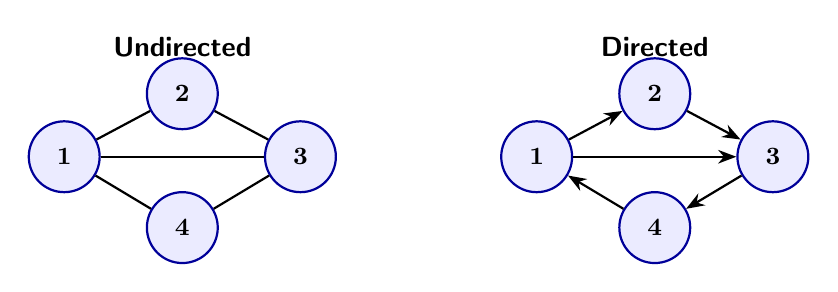
\begin{tikzpicture}[
  node/.style={circle, draw=blue!60!black, fill=blue!8, thick, minimum size=9mm, font=\small\bfseries},
  >=Stealth, thick
]
\node[font=\bfseries\sffamily] at (1.5, 2.4) {Undirected};
\node[node] (u1) at (0,1)   {1};
\node[node] (u2) at (1.5,1.8) {2};
\node[node] (u3) at (3,1)   {3};
\node[node] (u4) at (1.5,0.1) {4};
\draw (u1)--(u2); \draw (u2)--(u3); \draw (u3)--(u4); \draw (u4)--(u1); \draw (u1)--(u3);

\node[font=\bfseries\sffamily] at (7.5, 2.4) {Directed};
\node[node] (d1) at (6,1)   {1};
\node[node] (d2) at (7.5,1.8) {2};
\node[node] (d3) at (9,1)   {3};
\node[node] (d4) at (7.5,0.1) {4};
\draw[->] (d1)--(d2); \draw[->] (d2)--(d3); \draw[->] (d3)--(d4);
\draw[->] (d4)--(d1); \draw[->] (d1)--(d3);
\end{tikzpicture}
\end{center}

\subsection{Weighted Graphs and Multigraphs}

\begin{conceptbox}{Weighted Graph and Multigraph}
\begin{itemize}[noitemsep]
    \item \textbf{Weighted graph:} A function $w: \mathcal{E} \to \mathbb{R}$ assigns a scalar weight $w_{ij}$ to each edge. The notation $w_{ij}$ means: ``the weight of the edge between node $i$ and node $j$.'' Weights may encode contact duration, transmission probability, or social tie strength.
    \item \textbf{Multigraph:} Multiple edges may connect the same pair of nodes (e.g.\ three separate conversations between the same two people on a given day).
    \item \textbf{Simple graph:} No self-loops ($(v,v) \notin \mathcal{E}$) and no multi-edges. Unless stated otherwise, we work with simple graphs.
\end{itemize}
\end{conceptbox}

\subsection{Subgraphs and Induced Subgraphs}

\begin{conceptbox}{Subgraph and Induced Subgraph}
Given $G = (\mathcal{V}, \mathcal{E})$:
\begin{itemize}[noitemsep]
    \item A \textbf{subgraph} $H = (\mathcal{V}', \mathcal{E}')$ satisfies $\mathcal{V}' \subseteq \mathcal{V}$ and $\mathcal{E}' \subseteq \mathcal{E} \cap (\mathcal{V}' \times \mathcal{V}')$.
    \item The \textbf{induced subgraph} $G[\mathcal{V}']$ contains \emph{all} edges of $G$ whose both endpoints lie in $\mathcal{V}'$: $\mathcal{E}' = \{(u,v) \in \mathcal{E} \mid u,v \in \mathcal{V}'\}$.
\end{itemize}
The \textbf{infected subgraph} at observation time $T$ is the induced subgraph on the infected nodes --- the ``crime scene'' our source-detection algorithms must analyse.
\end{conceptbox}

\begin{analogybox}{Subgraph as a Zoomed Map}
Think of a road atlas. The full map is $G$. If you zoom in on one city, you see all roads that begin and end within that city: that is the induced subgraph $G[\mathcal{V}']$. A non-induced subgraph would be like drawing only \emph{some} of those roads.
\end{analogybox}

% =============================================================================
\section{Matrix Representations}
\label{sec:matrix_representations}
% =============================================================================

\begin{conceptbox}{Building Blocks: What Is a Matrix?}
A \textbf{matrix} is a rectangular array of numbers arranged in \textbf{rows} (horizontal lines) and \textbf{columns} (vertical lines). A matrix with $n$ rows and $n$ columns is an $n \times n$ matrix.

The entry in \textbf{row $i$} and \textbf{column $j$} of matrix $\mathbf{M}$ is written $M_{ij}$. For example:
\[
\mathbf{M} = \begin{pmatrix} 5 & 0 & 2 \\ 0 & 3 & 1 \\ 2 & 1 & 4 \end{pmatrix}
\]
Here $M_{12} = 0$ (row 1, column 2), $M_{23} = 1$ (row 2, column 3), $M_{31} = 2$ (row 3, column 1).

A \textbf{diagonal matrix} has non-zero entries \emph{only} on the main diagonal (where row index equals column index). We write $\mathrm{diag}(d_1, d_2, \ldots, d_n)$ for the diagonal matrix with values $d_1, \ldots, d_n$.
\end{conceptbox}

\subsection{The Six-Node Running Example}

\begin{examplebox}{Running Example: Graph $G_6$}
\label{ex:g6}
Undirected graph on six nodes $\{1,2,3,4,5,6\}$ with edges:
\[
\mathcal{E} = \{\{1,2\},\, \{1,3\},\, \{2,3\},\, \{2,4\},\, \{3,5\},\, \{4,5\},\, \{4,6\},\, \{5,6\}\}
\]
$n=6$, $m=8$. Degrees: $k_1=2,\; k_2=3,\; k_3=3,\; k_4=3,\; k_5=3,\; k_6=2$.

\begin{center}
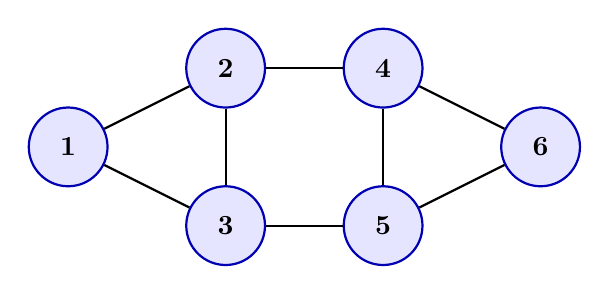
\begin{tikzpicture}[
  node/.style={circle, draw=blue!70!black, fill=blue!10, thick, minimum size=10mm, font=\bfseries},
  >=Stealth, thick
]
\node[node] (n1) at (0, 0)    {1};
\node[node] (n2) at (2, 1)    {2};
\node[node] (n3) at (2,-1)    {3};
\node[node] (n4) at (4, 1)    {4};
\node[node] (n5) at (4,-1)    {5};
\node[node] (n6) at (6, 0)    {6};
\draw (n1)--(n2); \draw (n1)--(n3); \draw (n2)--(n3); \draw (n2)--(n4);
\draw (n3)--(n5); \draw (n4)--(n5); \draw (n4)--(n6); \draw (n5)--(n6);
\end{tikzpicture}
\end{center}

Verification: $\sum_i k_i = 2+3+3+3+3+2 = 16 = 2 \times 8 = 2m$ \checkmark
\end{examplebox}

\begin{analogybox}{$G_6$ as a Disease Scenario}
Nodes 1--6 are six people. Edges are contacts. If person 1 is Patient Zero and infects person 2, person 2 can spread to 3 and 4. Person 3 can spread to 5, who can reach 6. The graph defines every possible transmission route. Our goal: given the final outbreak pattern (who is infected), can we infer that node 1 was the source?
\end{analogybox}

\subsection{Adjacency Matrix}

\begin{mathbox}{Adjacency Matrix $\mathbf{A}$}
\textbf{What it represents:} $A_{ij} = 1$ means nodes $i$ and $j$ are connected; $A_{ij} = 0$ means no direct edge.

\textbf{Formal definition:}
\[
A_{ij} = \begin{cases} 1 & \{i,j\} \in \mathcal{E} \\ 0 & \text{otherwise} \end{cases}, \qquad \mathbf{A} \in \{0,1\}^{n \times n}
\]

For undirected graphs, $\mathbf{A}$ is \textbf{symmetric}: $A_{ij} = A_{ji}$ (an edge goes both ways). For weighted graphs, replace $1$ by weight $w_{ij}$.

\textbf{Degrees from $\mathbf{A}$:} $k_i = \sum_{j=1}^n A_{ij}$ (row sum = number of 1s in row $i$).

\textbf{Powers of $\mathbf{A}$:} The entry $[\mathbf{A}^{\ell}]_{ij}$ counts the number of walks of length $\ell$ from $i$ to $j$. This algebraic fact underlies why $L$-layer GNNs give nodes access to their $L$-hop neighbourhood.
\end{mathbox}

\begin{examplebox}{Building the Adjacency Matrix for $G_6$}
Fill the $6 \times 6$ matrix: row $i$ gets a $1$ in column $j$ when edge $\{i,j\}$ exists.
\[
\mathbf{A} = \begin{pmatrix}
0 & 1 & 1 & 0 & 0 & 0 \\
1 & 0 & 1 & 1 & 0 & 0 \\
1 & 1 & 0 & 0 & 1 & 0 \\
0 & 1 & 0 & 0 & 1 & 1 \\
0 & 0 & 1 & 1 & 0 & 1 \\
0 & 0 & 0 & 1 & 1 & 0
\end{pmatrix}
\]
Symmetry check: $A_{12}=1=A_{21}$ \checkmark. \quad Degree check for node 2: row 2 sums to $1+0+1+1+0+0=3=k_2$ \checkmark.
\end{examplebox}

\subsection{Degree Matrix}

\begin{mathbox}{Degree Matrix $\mathbf{D}$}
\textbf{What it represents:} Diagonal matrix recording how many connections each node has.
\[
D_{ii} = k_i = \sum_{j} A_{ij}, \qquad D_{ij} = 0 \text{ for } i \neq j.
\]
For $G_6$: $\mathbf{D} = \mathrm{diag}(2,\, 3,\, 3,\, 3,\, 3,\, 2)$.
\end{mathbox}

\subsection{The Graph Laplacian}

The Laplacian is arguably the single most important matrix in graph theory. It encodes both the degree of every node and the connectivity structure of the graph. To understand it, we first need matrix subtraction.

\begin{conceptbox}{Matrix Subtraction: $\mathbf{D} - \mathbf{A}$}
To subtract two same-size matrices, subtract their corresponding entries:
$(\mathbf{D} - \mathbf{A})_{ij} = D_{ij} - A_{ij}$.

Example for $G_6$ at position $(1,1)$: $D_{11} - A_{11} = 2 - 0 = 2$.
At position $(1,2)$: $D_{12} - A_{12} = 0 - 1 = -1$.
\end{conceptbox}

\begin{mathbox}{Graph Laplacian $\mathbf{L}$}
\[
\mathbf{L} = \mathbf{D} - \mathbf{A}
\]
\textbf{Reading aloud:} ``The Laplacian $L$ equals degree matrix $D$ minus adjacency matrix $A$, subtracted entry-by-entry.''

Each entry:
\[
L_{ij} = \begin{cases}
k_i & i = j \quad \text{(put the degree on the diagonal)}\\
-1  & \{i,j\} \in \mathcal{E} \quad \text{(put $-1$ where there is an edge)}\\
0   & \text{otherwise}
\end{cases}
\]

\textbf{Key properties:}
\begin{itemize}[noitemsep]
    \item $\mathbf{L}$ is \textbf{symmetric} (inherited from $\mathbf{A}$).
    \item Every row sums to zero: on the diagonal we have $k_i$; the off-diagonal $-1$s count the same $k_i$ neighbours. They cancel exactly.
    \item $\mathbf{L}$ is \textbf{positive semi-definite}: all eigenvalues $0 = \lambda_1 \leq \lambda_2 \leq \cdots \leq \lambda_n$.
    \item Multiplicity of eigenvalue $0$ = number of connected components.
    \item For any vector $\mathbf{f} \in \mathbb{R}^n$: $\mathbf{f}^\top \mathbf{L} \mathbf{f} = \sum_{\{i,j\} \in \mathcal{E}} (f_i - f_j)^2 \geq 0$ measures total variation of signal $\mathbf{f}$ across edges. Here $\mathbf{f}^\top$ (``$f$-transpose'') turns a column vector into a row vector.
\end{itemize}
\end{mathbox}

\begin{examplebox}{Computing $\mathbf{L}$ for $G_6$ Step by Step}
$\mathbf{L} = \mathbf{D} - \mathbf{A}$:
\[
\mathbf{L} = \begin{pmatrix}
 2 & -1 & -1 &  0 &  0 &  0 \\
-1 &  3 & -1 & -1 &  0 &  0 \\
-1 & -1 &  3 &  0 & -1 &  0 \\
 0 & -1 &  0 &  3 & -1 & -1 \\
 0 &  0 & -1 & -1 &  3 & -1 \\
 0 &  0 &  0 & -1 & -1 &  2
\end{pmatrix}
\]
Row sums: $2-1-1=0$ \checkmark, $-1+3-1-1=0$ \checkmark, etc. Symmetric \checkmark.
\end{examplebox}

\begin{analogybox}{The Laplacian as a Resistance Network}
Replace every edge with a unit resistor. Inject current into node $i$ and remove it from node $j$. The resulting voltage differences are governed by $\mathbf{L}$. It is the discrete analogue of the continuous Laplacian $\nabla^2$ from physics, measuring how much a function ``spreads out'' relative to its neighbourhood average.
\end{analogybox}

\subsection{Normalised Laplacians}

Raw eigenvalues of $\mathbf{L}$ scale with the maximum degree. For heterogeneous networks (e.g.\ scale-free), this makes spectral comparison across graphs difficult. Normalised Laplacians fix this by rescaling each entry by the degrees of its endpoint nodes.

Before writing the formula, we must understand what $\mathbf{D}^{-1/2}$ means.

\begin{mathbox}{Powers of a Diagonal Matrix: $\mathbf{D}^{-1/2}$ Explained from Scratch}

\textbf{Step 1: Powers of a number.}
For any positive number $d$: $d^{1/2} = \sqrt{d}$ (square root), $d^{-1} = 1/d$ (reciprocal), $d^{-1/2} = 1/\sqrt{d}$ (reciprocal of square root).

\textbf{Step 2: Powers of a diagonal matrix.}
For a diagonal matrix, raise each diagonal entry to the power, leaving zeros unchanged:
\[
\mathbf{D} = \mathrm{diag}(d_1, d_2, \ldots, d_n) \implies \mathbf{D}^p = \mathrm{diag}(d_1^p, d_2^p, \ldots, d_n^p)
\]

\textbf{Step 3: Computing $\mathbf{D}^{-1/2}$ for $G_6$.}
$\mathbf{D} = \mathrm{diag}(2, 3, 3, 3, 3, 2)$, so:
\[
\mathbf{D}^{-1/2} = \mathrm{diag}\!\left(\frac{1}{\sqrt{2}},\, \frac{1}{\sqrt{3}},\, \frac{1}{\sqrt{3}},\, \frac{1}{\sqrt{3}},\, \frac{1}{\sqrt{3}},\, \frac{1}{\sqrt{2}}\right)
\approx \mathrm{diag}(0.707,\, 0.577,\, 0.577,\, 0.577,\, 0.577,\, 0.707)
\]

\textbf{Why $-1/2$ specifically?}
Multiplying $\mathbf{D}^{-1/2}$ on the left \emph{and} right of $\mathbf{L}$ divides each entry $L_{ij}$ by $\sqrt{k_i} \cdot \sqrt{k_j}$. This rescales the matrix so high-degree nodes do not dominate the spectrum. Multiplying on both sides (the ``sandwich'') preserves symmetry.
\end{mathbox}

\begin{mathbox}{Normalised Laplacians}
\textbf{Symmetric (spectral) normalised Laplacian:}
\[
\tilde{\mathbf{L}}_{\mathrm{sym}} = \mathbf{D}^{-1/2}\,\mathbf{L}\,\mathbf{D}^{-1/2}
= \mathbf{I} - \mathbf{D}^{-1/2}\mathbf{A}\mathbf{D}^{-1/2}
\]
\textbf{Reading aloud:} ``Take $\mathbf{D}^{-1/2}$ (reciprocal square-roots of degrees on diagonal), multiply on the left of $\mathbf{L}$, then multiply $\mathbf{D}^{-1/2}$ on the right. Eigenvalues lie in $[0,2]$.'' The identity matrix $\mathbf{I}$ has all 1s on the diagonal.

\textbf{Random-walk normalised Laplacian:}
\[
\tilde{\mathbf{L}}_{\mathrm{rw}} = \mathbf{D}^{-1}\mathbf{L} = \mathbf{I} - \mathbf{D}^{-1}\mathbf{A}
\]
Here $[\mathbf{D}^{-1}\mathbf{A}]_{ij} = A_{ij}/k_i$ is the transition probability of a random walker at node $i$ moving to node $j$ in one step.

\textbf{GCN renormalised adjacency} \cite{kipf2017}:
\[
\hat{\mathbf{A}} = \tilde{\mathbf{D}}^{-1/2}\tilde{\mathbf{A}}\tilde{\mathbf{D}}^{-1/2},
\qquad \tilde{\mathbf{A}} = \mathbf{A} + \mathbf{I}
\]
Adding $\mathbf{I}$ (self-loops) ensures a node also receives its own features during aggregation.
\end{mathbox}

\begin{examplebox}{Off-Diagonal Entries of $\tilde{\mathbf{L}}_{\mathrm{sym}}$ for $G_6$}
The formula $[\tilde{\mathbf{L}}_{\mathrm{sym}}]_{ij} = -A_{ij}/\sqrt{k_i \cdot k_j}$ gives:
\begin{center}
\begin{tabular}{lcccc}
\toprule
Edge & $k_i$ & $k_j$ & $\sqrt{k_i k_j}$ & Entry \\
\midrule
$\{1,2\},\{1,3\},\{4,6\},\{5,6\}$ & 2 & 3 & $\sqrt{6}\approx 2.449$ & $-0.408$ \\
$\{2,3\},\{2,4\},\{3,5\},\{4,5\}$ & 3 & 3 & $3$ & $-0.333$ \\
\bottomrule
\end{tabular}
\end{center}
All diagonal entries equal 1. All eigenvalues lie in $[0, 2]$ regardless of degree heterogeneity.
\end{examplebox}

% =============================================================================
\section{Spectral Graph Theory}
\label{sec:spectral}
% =============================================================================

\begin{conceptbox}{Building Blocks for This Section}
New symbols:
\begin{itemize}[noitemsep]
    \item $\lambda$ (Greek ``lambda'') --- an eigenvalue (a scalar)
    \item $\mathbf{u}$ --- an eigenvector (a special vector)
    \item $\mathbf{U}$ --- matrix of all eigenvectors (columns are eigenvectors)
    \item $\boldsymbol{\Lambda}$ (capital Greek ``Lambda'') --- diagonal matrix of eigenvalues
    \item $\mathbf{U}^\top$ --- transpose of $\mathbf{U}$: swap rows and columns
    \item $\hat{\mathbf{f}}$ --- hat notation: ``$f$ in frequency domain''
    \item $\odot$ --- element-wise multiplication: $(a \odot b)_i = a_i \cdot b_i$
    \item $\mathbb{R}^n$ --- the set of all $n$-dimensional real-valued vectors
\end{itemize}
\end{conceptbox}

\subsection{Eigenvalues and Eigenvectors: Starting from Scratch}

\begin{mathbox}{What Is an Eigenvector?}
\textbf{Core idea:} Multiplying a matrix $\mathbf{M}$ by most vectors rotates \emph{and} scales them. For special vectors called \textbf{eigenvectors}, multiplying only \emph{scales} (stretches or shrinks) --- the direction stays the same.

Formally, $\mathbf{u} \neq \mathbf{0}$ is an eigenvector of $\mathbf{M}$ with eigenvalue $\lambda$ if:
\[
\mathbf{M}\mathbf{u} = \lambda\, \mathbf{u}
\]
``Matrix $M$ times vector $u$ equals lambda times vector $u$.''

\textbf{Numerical $2\times 2$ example:}
\[
\mathbf{M} = \begin{pmatrix} 2 & 1 \\ 0 & 3 \end{pmatrix}, \quad \mathbf{u} = \begin{pmatrix} 1 \\ 1 \end{pmatrix}
\implies
\mathbf{M}\mathbf{u} = \begin{pmatrix} 3 \\ 3 \end{pmatrix} = 3 \begin{pmatrix} 1 \\ 1 \end{pmatrix} = 3\,\mathbf{u}
\]
So $\mathbf{u} = (1,1)^\top$ is an eigenvector with eigenvalue $\lambda = 3$. The vector was scaled by 3 but kept its direction.
\end{mathbox}

\begin{mathbox}{Eigendecomposition of $\mathbf{L}$}
Because $\mathbf{L}$ is real and symmetric, it has a complete orthonormal set of eigenvectors (``orthonormal'' = mutually perpendicular, each with length 1):
\[
\mathbf{L} = \mathbf{U}\,\boldsymbol{\Lambda}\,\mathbf{U}^\top, \qquad
\boldsymbol{\Lambda} = \mathrm{diag}(\lambda_1, \lambda_2, \dots, \lambda_n), \quad
0 = \lambda_1 \leq \lambda_2 \leq \cdots \leq \lambda_n.
\]
$\mathbf{U}$ stacks all eigenvectors as columns; $\mathbf{U}^\top\mathbf{U} = \mathbf{I}$ (orthogonal matrix).

\textbf{Why $\lambda_1 = 0$ always?} Consider the all-ones vector $\mathbf{1} = (1,\ldots,1)^\top$. Since every row of $\mathbf{L}$ sums to zero, $\mathbf{L}\mathbf{1} = \mathbf{0} = 0 \cdot \mathbf{1}$. So $\mathbf{1}$ is an eigenvector with eigenvalue 0. Physically: a uniform signal (same value everywhere) has zero variation across edges.

\textbf{Interpretation:}
\begin{itemize}[noitemsep]
    \item \textbf{Small eigenvalues} $\to$ smooth signals (vary slowly across edges)
    \item \textbf{Large eigenvalues} $\to$ rapidly oscillating signals (high frequency)
    \item \textbf{Spectral gap} $\lambda_2$: larger $\lambda_2$ means better-connected graph
\end{itemize}
\end{mathbox}

\begin{analogybox}{Eigenvalues as Musical Notes}
The eigenvectors of $\mathbf{L}$ are the ``pure tones'' of the graph. The all-ones eigenvector ($\lambda_1 = 0$) is the lowest note---a constant hum. Higher eigenvalues correspond to higher-frequency tones oscillating rapidly across the graph. Just as any piece of music decomposes into pure tones, any epidemic pattern decomposes into these eigenvectors.
\end{analogybox}

\subsection{Algebraic Connectivity and the Fiedler Value}

\begin{keyinsight}{The Fiedler Value $\lambda_2$}
The second-smallest eigenvalue $\lambda_2$ of $\mathbf{L}$ is the \textbf{algebraic connectivity} (Fiedler value, 1973).

\textbf{Intuition:} A network with a single bottleneck (one bridge connecting two halves) has tiny $\lambda_2$. A tightly-knit network with many redundant paths has large $\lambda_2$.

\textbf{Formal properties:}
\begin{itemize}[noitemsep]
    \item $\lambda_2 > 0$ $\iff$ $G$ is \textbf{connected}.
    \item Larger $\lambda_2$ $\to$ fewer bottlenecks $\to$ faster, wider spreading.
    \item The \textbf{Fiedler vector} $\mathbf{u}_2$ partitions the graph into two communities by sign ($[\mathbf{u}_2]_i > 0$ vs $< 0$) --- the basis of spectral clustering.
\end{itemize}

For source detection: high-$\lambda_2$ networks are harder cases because infection spreads in all directions quickly, making the outbreak look symmetric regardless of the source location.
\end{keyinsight}

\subsection{The Graph Fourier Transform}

\begin{analogybox}{From Audio Fourier Transform to Graph Fourier Transform}
The audio Fourier Transform decomposes a sound wave $f(t)$ into pure sine waves: ``how much of each frequency is present?''

The graph analogy:
\begin{itemize}[noitemsep]
    \item Time-domain signal $f(t)$ $\to$ Graph signal $\mathbf{f} \in \mathbb{R}^n$ (one value per node)
    \item Sine wave at frequency $\omega$ $\to$ Eigenvector $\mathbf{u}_k$ (the $k$-th graph frequency)
    \item Frequency coefficient $\hat{f}(\omega)$ $\to$ Inner product $\hat{f}_k = \mathbf{u}_k^\top \mathbf{f}$ (how much the signal resembles frequency $k$)
\end{itemize}
\end{analogybox}

\begin{mathbox}{Graph Fourier Transform (GFT)}
A \textbf{graph signal} is a vector $\mathbf{f} \in \mathbb{R}^n$ where $f_i$ is the value at node $i$ (e.g.\ 1 if infected, 0 if not).

\textbf{Forward GFT:} $\hat{\mathbf{f}} = \mathbf{U}^\top \mathbf{f}$ \quad (node domain $\to$ frequency domain)

$\hat{f}_k = \mathbf{u}_k^\top \mathbf{f}$ measures how much the signal ``resonates'' with the $k$-th graph frequency.

\textbf{Inverse GFT:} $\mathbf{f} = \mathbf{U}\hat{\mathbf{f}} = \sum_{k=1}^{n} \hat{f}_k\, \mathbf{u}_k$ \quad (frequency domain $\to$ node domain)

\textbf{Graph convolution} with filter $\mathbf{g}$:
\[
\mathbf{f} * \mathbf{g} = \mathbf{U}\!\left(\hat{\mathbf{f}} \odot \hat{\mathbf{g}}\right) = \mathbf{U}\,\mathrm{diag}(\hat{g}_1, \dots, \hat{g}_n)\,\mathbf{U}^\top\mathbf{f}
\]
where $\odot$ is element-wise multiplication: $(\hat{\mathbf{f}} \odot \hat{\mathbf{g}})_k = \hat{f}_k \cdot \hat{g}_k$.

\textbf{A GNN layer is a learnable spectral filter:} the parameters $\hat{g}_k$ are trained to emphasise the frequency components most useful for source detection.

\textbf{The computational problem:} Explicit eigendecomposition costs $O(n^3)$ --- prohibitive for large networks. Polynomial approximations solve this.
\end{mathbox}

\subsection{Chebyshev Polynomial Approximation}

\begin{mathbox}{What Is a Polynomial?}
A polynomial in variable $x$ is: $p(x) = c_0 + c_1 x + c_2 x^2 + \cdots + c_K x^K$.

When we write $p(\mathbf{L})$, we replace $x$ by the matrix $\mathbf{L}$:
$p(\mathbf{L}) = c_0 \mathbf{I} + c_1 \mathbf{L} + c_2 \mathbf{L}^2 + \cdots + c_K \mathbf{L}^K$.

Computing $\mathbf{L}^k\mathbf{f}$ iteratively costs $O(k \cdot m)$ (sparse matrix-vector products), far cheaper than the $O(n^3)$ eigendecomposition.
\end{mathbox}

\begin{mathbox}{Chebyshev Polynomials on Graphs}
Chebyshev polynomials $T_k(x)$ provide the \emph{best approximation} to smooth functions on $[-1,1]$ in the minimax sense. They are defined by the recurrence:
\[
T_0(x) = 1, \quad T_1(x) = x, \quad T_k(x) = 2x\,T_{k-1}(x) - T_{k-2}(x), \quad k \geq 2
\]

\textbf{First four polynomials:}
$T_0(x) = 1$, $T_1(x) = x$, $T_2(x) = 2x^2 - 1$, $T_3(x) = 4x^3 - 3x$.

\textbf{Numerical check at $x = 0.5$:}
$T_0(0.5)=1$, $T_1(0.5)=0.5$, $T_2(0.5)=2(0.25)-1=-0.5$, $T_3(0.5)=4(0.125)-1.5=-1.0$.

\textbf{Applying to graphs:} Rescale eigenvalues to $[-1,1]$: $\hat{\mathbf{L}} = \frac{2}{\lambda_{\max}}\mathbf{L} - \mathbf{I}$. Approximate a graph filter as:
\[
\mathbf{g}_\theta(\mathbf{L}) \approx \sum_{k=0}^{K} \theta_k\, T_k(\hat{\mathbf{L}})
\]
Each term $T_k(\hat{\mathbf{L}})\mathbf{f}$ is computed recursively in $O(K \cdot m)$ time --- no eigendecomposition. This is the foundation of \textbf{ChebNet} and \textbf{GCN} \cite{kipf2017}.

\textbf{Key insight:} A filter of order $K$ aggregates information from at most $K$ hops away. Setting $K=1$ with $\lambda_{\max} \approx 2$ yields the GCN layer.
\end{mathbox}

% =============================================================================
\section{Key Network Metrics}
\label{sec:network_metrics}
% =============================================================================

\begin{conceptbox}{Building Blocks for This Section}
New symbols:
\begin{itemize}[noitemsep]
    \item $P(k)$ --- degree distribution: probability that a random node has degree $k$
    \item $\binom{k}{2} = \frac{k(k-1)}{2}$ --- ``$k$ choose 2'': number of ways to choose 2 items from $k$
    \item $\sigma(s,t)$ --- number of shortest paths between nodes $s$ and $t$
    \item $d(v, u)$ --- shortest-path distance (number of edges on shortest path)
    \item $\alpha$ (Greek ``alpha'') --- damping factor in PageRank, typically $0.85$
    \item $\gamma$ (Greek ``gamma'') --- exponent in power-law degree distribution
\end{itemize}
\end{conceptbox}

\subsection{Degree Distribution}

\begin{conceptbox}{Degree Distribution $P(k)$}
\[
P(k) = \frac{|\{v \in \mathcal{V} \mid k_v = k\}|}{n}
\]
\textbf{Reading aloud:} ``$P(k)$ is the number of nodes with degree $k$, divided by the total number of nodes $n$.''

Two important shapes:
\begin{itemize}[noitemsep]
    \item \textbf{Poisson} (Erd\H{o}s-R\'enyi): narrow, symmetric around the mean; no hubs.
    \item \textbf{Power-law} $P(k) \sim k^{-\gamma}$ (scale-free): heavy tail; few super-connected hubs; the epidemic threshold effectively vanishes.
\end{itemize}
\end{conceptbox}

\subsection{Clustering Coefficient}

\begin{mathbox}{Local Clustering Coefficient}
\textbf{What it measures:} ``Are my friends also friends with each other?''
\[
C_v = \frac{|\{(u,w) \in \mathcal{E} \mid u,w \in \mathcal{N}(v)\}|}{\binom{k_v}{2}} = \frac{2 \cdot |\triangle_v|}{k_v(k_v-1)}
\]
Numerator: actual edges among $v$'s neighbours. Denominator: maximum possible edges among $k_v$ neighbours. $|\triangle_v|$ = triangles containing $v$.

$\bar{C} = \frac{1}{n}\sum_v C_v$ is the global clustering coefficient. High clustering means tightly-knit local communities.
\end{mathbox}

\subsection{Centrality Measures}

\begin{mathbox}{Betweenness and Closeness Centrality}
\textbf{Betweenness centrality:}
\[
C_B(v) = \sum_{\substack{s \neq t \\ s,t \neq v}} \frac{\sigma(s,t \mid v)}{\sigma(s,t)}
\]
$\sigma(s,t)$ = total shortest paths from $s$ to $t$; $\sigma(s,t \mid v)$ = those passing through $v$.
High betweenness identifies \textbf{bridge nodes}: removing them fragments the graph.

\textbf{Closeness centrality:}
\[
C_C(v) = \frac{n-1}{\sum_{u \neq v} d(v,u)}
\]
Nodes with high closeness are geometrically central. In epidemics, they are reached early --- strong source candidates.
\end{mathbox}

\begin{analogybox}{Betweenness as a Toll Booth}
Every shortest path is a delivery truck. Betweenness counts how many trucks pass through your city. High betweenness = removing this node (quarantine) disrupts the most routes. In epidemics, super-spreaders often bridge otherwise separate communities.
\end{analogybox}

\subsection{PageRank}

\begin{mathbox}{PageRank}
Models a random web surfer: with probability $\alpha$ follow a random outgoing link, with probability $1-\alpha$ teleport to a random page. Stationary probability at node $v$:
\[
\mathrm{PR}(v) = \frac{1-\alpha}{n} + \alpha \sum_{u \in \mathcal{N}^{\mathrm{in}}(v)} \frac{\mathrm{PR}(u)}{k_u^{\mathrm{out}}}
\]
Damping factor $\alpha \approx 0.85$. In source detection, backwards PageRank can identify likely epidemic origins.
\end{mathbox}

\subsection{Worked Metrics for $G_6$}

\begin{examplebox}{All Metrics for $G_6$}
\textbf{Clustering coefficients:}
Node 1 ($k=2$, neighbours $\{2,3\}$, edge $\{2,3\} \in \mathcal{E}$): $C_1 = 1.0$.
Node 2 ($k=3$, neighbours $\{1,3,4\}$, edge $\{1,3\} \in \mathcal{E}$): $C_2 = 1/3 \approx 0.33$.
By symmetry: $C_3 = C_4 = C_5 \approx 0.33$, $C_6 = 1.0$.
$\bar{C} \approx 0.556$.

\textbf{Closeness centrality:}
\begin{center}
\begin{tabular}{cccc}
\toprule
Node & Sum of distances & $C_C(v) = 5/\text{sum}$ & Interpretation \\
\midrule
1, 6 & 9 & $\approx 0.56$ & Peripheral \\
2, 3, 4, 5 & 7 & $\approx 0.71$ & Central \\
\bottomrule
\end{tabular}
\end{center}

\textbf{Degree distribution:} $P(2) \approx 0.33$, $P(3) \approx 0.67$, $\langle k \rangle \approx 2.67$.

\textbf{Epidemic implication:} The symmetry of $G_6$ under exchange $\{1\!\leftrightarrow\!6,\, 2\!\leftrightarrow\!5,\, 3\!\leftrightarrow\!4\}$ means outbreaks from node 1 and node 6 are structurally indistinguishable. This is exactly what makes source detection hard: multiple source hypotheses produce statistically identical patterns.
\end{examplebox}

% =============================================================================
\section{Network Generation Models}
\label{sec:network_models}
% =============================================================================

\begin{conceptbox}{Building Blocks for This Section}
\begin{itemize}[noitemsep]
    \item $G(n,p)$ --- Erd\H{o}s-R\'enyi random graph: $n$ nodes, each possible edge included with probability $p$
    \item $\langle k \rangle$ --- mean (expected) degree; angle brackets denote an average
    \item $\Pi(v)$ (capital Greek ``pi'') --- attachment probability in the BA model
    \item $\beta_{\mathrm{rew}}$ --- rewiring probability in the WS model
    \item $O(\cdot)$ --- Big-O notation: at most this rate of growth
\end{itemize}
\end{conceptbox}

\subsection{Erd\H{o}s-R\'{e}nyi Random Graphs}

\begin{conceptbox}{Erd\H{o}s-R\'{e}nyi $G(n,p)$}
$n$ nodes; each of the $\binom{n}{2}$ possible edges is included independently with probability $p$.

\textbf{Expected properties:}
\begin{itemize}[noitemsep]
    \item Mean degree: $\langle k \rangle \approx np$.
    \item Degree distribution: $\mathrm{Binomial}(n-1,p) \to \mathrm{Poisson}(\langle k \rangle)$ as $n \to \infty$.
    \item \textbf{Giant component threshold:} For $p < 1/n$: all components have size $O(\log n)$. For $p > 1/n$: a giant component of size $\Theta(n)$ emerges. This directly parallels the epidemic threshold.
    \item Diameter $\approx \ln n / \ln \langle k \rangle$.
\end{itemize}
\end{conceptbox}

\begin{keyinsight}{Why ER Is Our Primary Synthetic Benchmark}
All nodes in an ER graph are statistically equivalent. No structural shortcut helps identify the source. Any gain our GNN achieves on ER graphs must come from learning the epidemic spreading pattern itself---making ER the purest test of inference quality.
\end{keyinsight}

\subsection{Barab\'{a}si-Albert Preferential Attachment}

\begin{conceptbox}{Barab\'{a}si-Albert (BA) Model}
Generates scale-free networks through \textbf{preferential attachment}: new nodes connect to existing nodes with probability proportional to their degree:
\[
\Pi(v) = \frac{k_v}{\sum_{u} k_u}
\]
A node with degree 10 is twice as likely to be chosen as a node with degree 5.

\textbf{Result:} Power-law degree distribution $P(k) \sim k^{-3}$. Early nodes become hubs with degree $\langle k_i(T) \rangle \approx m\sqrt{T/t_i}$.
\end{conceptbox}

\subsection{Watts-Strogatz Small-World Networks}

\begin{conceptbox}{Watts-Strogatz (WS) Model}
Interpolates between a regular ring lattice (high clustering, large diameter) and a random graph (low clustering, small diameter).

\textbf{Algorithm:}
\begin{enumerate}[noitemsep]
    \item Start with a ring lattice: $n$ nodes, each connected to its $K$ nearest neighbours.
    \item For each edge, with probability $\beta_\mathrm{rew}$, \textbf{rewire} it to a random node.
\end{enumerate}

$\beta_\mathrm{rew} \approx 0.01$--$0.1$ gives the \textbf{small-world regime}: high clustering \emph{and} short diameter simultaneously.
\end{conceptbox}

\begin{analogybox}{Small World as a Flight Network}
A pure lattice is like a medieval road system: enormous diameter. Pure random is like teleportation booths: tiny diameter but no local structure. A small-world network is like the real airline system: dense local connections plus a few long-haul shortcuts collapsing the diameter. The same structure makes diseases both locally clustering and globally fast-spreading.
\end{analogybox}

\subsection{Visual Comparison and Table}

\begin{center}
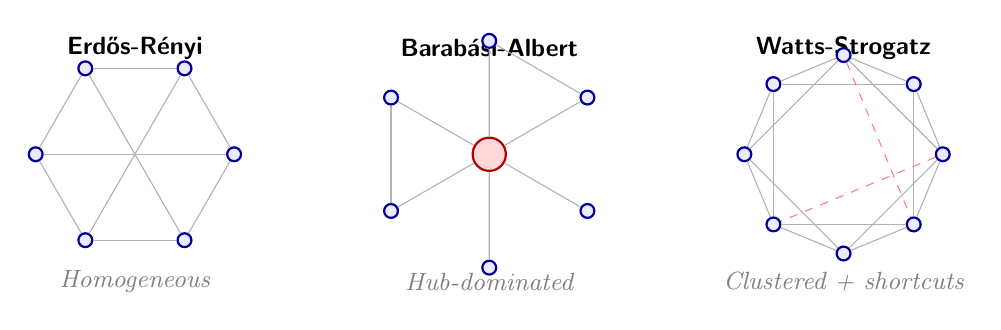
\begin{tikzpicture}[
  snode/.style={circle, draw=blue!60!black, fill=blue!8, minimum size=5pt, inner sep=0, thick},
  hnode/.style={circle, draw=red!70!black, fill=red!15, minimum size=8pt, inner sep=0, thick},
  scale=0.9
]
\node[font=\bfseries\sffamily\small] at (2.0, 3.0) {Erd\H{o}s-R\'{e}nyi};
\foreach \a in {0,...,5}{
  \node[snode] (er\a) at ({2.0+1.4*cos(60*\a)}, {1.5+1.4*sin(60*\a)}) {};
}
\foreach \a/\b in {0/1,1/2,2/3,3/4,4/5,5/0,0/3,1/4,2/5}{
  \draw[gray!60, thin] (er\a)--(er\b);
}
\node[font=\bfseries\sffamily\small] at (7.0, 3.0) {Barab\'{a}si-Albert};
\node[hnode, minimum size=12pt] (ba0) at (7.0, 1.5) {};
\foreach \i in {1,...,6}{
  \node[snode] (ba\i) at ({7.0+1.6*cos(60*\i-30)}, {1.5+1.6*sin(60*\i-30)}) {};
  \draw[gray!60, thin] (ba0)--(ba\i);
}
\draw[gray!60,thin] (ba1)--(ba2); \draw[gray!60,thin] (ba3)--(ba4);
\node[font=\bfseries\sffamily\small] at (12.0, 3.0) {Watts-Strogatz};
\foreach \i in {0,...,7}{
  \node[snode] (ws\i) at ({12.0+1.4*cos(45*\i)}, {1.5+1.4*sin(45*\i)}) {};
}
\foreach \i/\j in {0/1,1/2,2/3,3/4,4/5,5/6,6/7,7/0,0/2,1/3,2/4,3/5,4/6,5/7,6/0,7/1}{
  \draw[gray!60, thin] (ws\i)--(ws\j);
}
\draw[red!50, dashed, thin] (ws0)--(ws5);
\draw[red!50, dashed, thin] (ws2)--(ws7);
\node[font=\small\itshape, text=gray] at (2.0, -0.3) {Homogeneous};
\node[font=\small\itshape, text=gray] at (7.0, -0.3) {Hub-dominated};
\node[font=\small\itshape, text=gray] at (12.0, -0.3) {Clustered + shortcuts};
\end{tikzpicture}
\end{center}

The large red node in the BA diagram is the hub. The dashed red lines in the WS diagram are the rewired ``shortcut'' edges.

\begin{table}[H]
\centering
\caption{Comparison of standard network generation models.}
\label{tab:network_models}
\begin{tabular}{lllll}
\toprule
\textbf{Model} & \textbf{Degree dist.} & \textbf{Clustering} & \textbf{Diameter} & \textbf{Epidemic relevance} \\
\midrule
Erd\H{o}s-R\'{e}nyi & Poisson & Low $\sim K/n$ & $O(\ln n)$ & Mean-field baseline \\
Barab\'{a}si-Albert  & Power-law $k^{-3}$ & Moderate & $O(\ln n/\ln\ln n)$ & Super-spreader networks \\
Watts-Strogatz       & Peaked & High & $O(\ln n)$ & Real social/contact nets \\
Configuration        & Arbitrary & Depends & Depends & Null model \\
\bottomrule
\end{tabular}
\end{table}

% =============================================================================
\section{Comprehensive Worked Example: Building and Analysing $G_6$}
\label{sec:worked_example}
% =============================================================================

\begin{examplebox}{Step 1 --- Define the Graph}
$n=6$, $m=8$, density $\rho = 16/30 \approx 0.533$.
\end{examplebox}

\begin{examplebox}{Step 2 --- Adjacency and Degree Matrices}
\[
\mathbf{A} = \begin{pmatrix}
0&1&1&0&0&0\\1&0&1&1&0&0\\1&1&0&0&1&0\\0&1&0&0&1&1\\0&0&1&1&0&1\\0&0&0&1&1&0
\end{pmatrix}, \qquad
\mathbf{D} = \mathrm{diag}(2,3,3,3,3,2)
\]
$\mathrm{trace}(\mathbf{D}) = 16 = 2m$ \checkmark
\end{examplebox}

\begin{examplebox}{Step 3 --- Graph Laplacian}
$\mathbf{L} = \mathbf{D} - \mathbf{A}$:
\[
\mathbf{L} = \begin{pmatrix}
 2&-1&-1& 0& 0& 0\\
-1& 3&-1&-1& 0& 0\\
-1&-1& 3& 0&-1& 0\\
 0&-1& 0& 3&-1&-1\\
 0& 0&-1&-1& 3&-1\\
 0& 0& 0&-1&-1& 2
\end{pmatrix}
\]
Each row sums to zero \checkmark. Symmetric \checkmark. Diagonal entries equal degrees \checkmark.
\end{examplebox}

\begin{examplebox}{Step 4 --- $\mathbf{D}^{-1/2}$ and the Normalised Laplacian}
\[
\mathbf{D}^{-1/2} \approx \mathrm{diag}(0.707,\, 0.577,\, 0.577,\, 0.577,\, 0.577,\, 0.707)
\]
Off-diagonal entries: edges connecting degree-2 to degree-3 nodes give $-1/\sqrt{6} \approx -0.408$; degree-3 to degree-3 edges give $-1/3 \approx -0.333$. All eigenvalues in $[0,2]$.
\end{examplebox}

\begin{examplebox}{Steps 5--6 --- Metrics Summary}
\begin{center}
\begin{tabular}{ccccc}
\toprule
Node & Degree & $C_v$ & Closeness $C_C$ & Betweenness \\
\midrule
1 & 2 & 1.00 & 0.56 & 0 \\
2 & 3 & 0.33 & 0.71 & non-zero \\
3 & 3 & 0.33 & 0.71 & non-zero \\
4 & 3 & 0.33 & 0.71 & non-zero \\
5 & 3 & 0.33 & 0.71 & non-zero \\
6 & 2 & 1.00 & 0.56 & 0 \\
\bottomrule
\end{tabular}
\end{center}
$\bar{C} \approx 0.556$. Mean degree $\langle k \rangle \approx 2.67$.
\end{examplebox}

\begin{keyinsight}{Why These Matrices Matter for GNNs}
Every GNN layer performs a variant of:
\[
\mathbf{H}^{(l+1)} = \sigma\!\left(\hat{\mathbf{A}}\,\mathbf{H}^{(l)}\,\mathbf{W}^{(l)}\right)
\]
where:
\begin{itemize}[noitemsep]
    \item $\mathbf{H}^{(l)} \in \mathbb{R}^{n \times d_l}$: feature matrix at layer $l$ (one row per node)
    \item $\hat{\mathbf{A}}$: normalised adjacency (e.g.\ $\mathbf{D}^{-1/2}\mathbf{A}\mathbf{D}^{-1/2}$); multiplying by $\hat{\mathbf{A}}$ aggregates neighbours' features
    \item $\mathbf{W}^{(l)} \in \mathbb{R}^{d_l \times d_{l+1}}$: learnable weight matrix
    \item $\sigma$: non-linear activation (e.g.\ ReLU: $\sigma(x) = \max(0,x)$)
\end{itemize}

What changes between GCN, GraphSAGE, GAT, and ChebNet is \emph{precisely} which matrix plays the role of $\hat{\mathbf{A}}$. Understanding the Laplacian and its spectral properties is not abstract mathematics: it directly determines what structural information flows through each layer of every model in \texttt{gnn/}.
\end{keyinsight}

% =============================================================================
\section{Chapter Summary}
% =============================================================================

\begin{conceptbox}{What We Have Established}
\begin{enumerate}[noitemsep]
    \item \textbf{Graphs} $G = (\mathcal{V}, \mathcal{E})$ encode contact networks. The degree $k_i$ counts a node's neighbours. The handshaking lemma: $\sum_i k_i = 2m$.
    \item \textbf{Matrices:} $\mathbf{A}$ ($A_{ij}=1$ if edge exists), $\mathbf{D}$ (diagonal matrix of degrees), $\mathbf{L} = \mathbf{D}-\mathbf{A}$ (Laplacian). Every row of $\mathbf{L}$ sums to zero.
    \item \textbf{$\mathbf{D}^{-1/2}$:} For a diagonal matrix, raise each diagonal entry to the power $-1/2$ (i.e., take $1/\sqrt{d_i}$). The normalised Laplacian $\tilde{\mathbf{L}}_{\mathrm{sym}} = \mathbf{D}^{-1/2}\mathbf{L}\mathbf{D}^{-1/2}$ has eigenvalues in $[0,2]$. For $G_6$: off-diagonal entries are $-0.408$ (for 2-3 degree edges) or $-0.333$ (for 3-3 degree edges).
    \item \textbf{Eigenvectors/eigenvalues:} $\mathbf{L}\mathbf{u} = \lambda\mathbf{u}$. Smallest eigenvalue $\lambda_1 = 0$ (all-ones vector). Fiedler value $\lambda_2 > 0$ iff connected.
    \item \textbf{GFT:} $\hat{\mathbf{f}} = \mathbf{U}^\top\mathbf{f}$ decomposes a graph signal into frequency components. Graph convolution is spectral filtering. Chebyshev polynomials ($T_0=1, T_1=x, T_k=2xT_{k-1}-T_{k-2}$) make this $O(K \cdot m)$ instead of $O(n^3)$.
    \item \textbf{Network metrics:} Degree distribution, clustering, betweenness/closeness centrality, PageRank characterise local and global structure. They serve as node features in GNN models.
    \item \textbf{Generation models:} ER (homogeneous), BA (hub-dominated, $P(k)\sim k^{-3}$), WS (small-world), Configuration (arbitrary degree sequence).
\end{enumerate}
\textbf{Coming up:} Chapter~2 lifts these static definitions into the temporal domain, introducing time-stamped contact sequences, time-respecting paths, and the causal structure that makes temporal GNNs both necessary and powerful.
\end{conceptbox}

\chapter{Temporal Networks: When Time Changes Everything}
\label{chap:temporal_networks}

\textit{This chapter builds the mathematical language of temporal networks from the ground up. We
start with a simple three-person story that makes the core problem immediately tangible, then
formalise every concept step by step. By the end you will be able to read temporal network
papers, compute reachability by hand, and understand exactly how the project codebase stores
and uses contact sequences.}

%=============================================================================
\section{Why Static Graphs Fail for Epidemics: The Phantom Path Problem}
\label{sec:phantom_paths}
%=============================================================================

\subsection{A Three-Person Story}

Imagine three people: Alice (A), Bob (B), and Carol (C). They meet as follows:

\begin{itemize}
    \item \textbf{Monday ($t = 1$):} Alice meets Bob. They shake hands.
    \item \textbf{Tuesday ($t = 2$):} Bob meets Carol. They share a meal.
    \item \textbf{Sunday ($t = 7$):} Carol meets Alice. They sit together at a concert.
\end{itemize}

Now suppose Bob was infected with a virus on Monday. The question an epidemiologist asks is:
\textit{who could Bob have infected, and through whom?}

\begin{examplebox}{Drawing the Static Graph}
If we draw a graph that simply records ``who has met whom'' (ignoring time), we get:

\medskip
\begin{center}
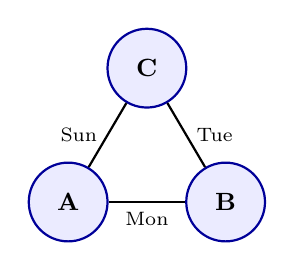
\begin{tikzpicture}[
  nd/.style={circle, draw=blue!60!black, fill=blue!8, thick,
             minimum size=10mm, font=\bfseries\small},
  >=Stealth, thick
]
  \node[nd] (A) at (0,0)   {A};
  \node[nd] (B) at (2,0)   {B};
  \node[nd] (C) at (1,1.7) {C};
  \draw (A) -- node[below, font=\scriptsize]{Mon} (B);
  \draw (B) -- node[right, font=\scriptsize]{Tue} (C);
  \draw (C) -- node[left,  font=\scriptsize]{Sun} (A);
\end{tikzpicture}
\end{center}

\medskip
In this static graph every pair of nodes is connected. A standard graph algorithm will
happily report the path $C \to A \to B$: Carol can infect Alice, and Alice can infect Bob.

But wait. Carol meets Alice on \textbf{Sunday} ($t=7$). Alice meets Bob on \textbf{Monday}
($t=1$). Sunday comes \textit{after} Monday. A pathogen cannot travel backwards in time. Carol
cannot infect Alice on Sunday and then have that infection arrive at Bob on Monday, six days
earlier.

The path $C \to A \to B$ \textbf{does not exist in reality}. It is a \textbf{phantom path}:
a path that looks valid in the static graph but is causally impossible because the edge
timestamps are in the wrong order.
\end{examplebox}

\begin{conceptbox}{Phantom Path}
A \textbf{phantom path} is a sequence of edges in the static projection of a temporal network
that appears to be a valid path but violates causal ordering: at least one edge in the sequence
has a timestamp that is \textit{earlier} than a preceding edge. An epidemic cannot travel
along a phantom path.
\end{conceptbox}

\begin{keyinsight}{The Core Problem with Static Graphs}
Static graphs tell you \textit{who has been in contact}, but not \textit{in what order}. For
epidemic spreading, order is everything: a virus can only move \emph{forward} in time. When a
static-graph algorithm suggests that Carol is a likely source because she is ``connected'' to
both Alice and Bob, it may be completely wrong---if Carol's contacts all happened after the
outbreak was already established, she cannot be the origin.

\textbf{This is why temporal networks exist}: they preserve the one piece of information that
static graphs discard---the timestamps that encode causality.
\end{keyinsight}

\subsection{A Brief History of Temporal Network Analysis}

Temporal or \textit{dynamic} graph models have been studied since at least the 1970s in the
context of communications networks, but the field gained coherent identity around 2012 with the
comprehensive review by \cite{holme2012temporal}. The key empirical observation motivating this
work was that real-world contact sequences exhibit strong non-Poissonian (``bursty'') timing:
inter-event times follow heavy-tailed rather than exponential distributions, with dramatic
consequences for how fast pathogens spread.

The formal study of \textit{time-respecting paths} and \textit{temporal reachability} was
pioneered by Kempe, Kleinberg, and Kumar \cite{kempe2000connectivity}, who established
complexity results for temporal connectivity problems. The event graph representation used in
this thesis derives from Saram\"{a}ki, Kivel\"{a}, and Karsai \cite{saramaki2019temporal},
covered in depth in Chapter~8.

%=============================================================================
\section{Formal Definition of a Temporal Network}
\label{sec:tn_definition}
%=============================================================================

We now give a precise mathematical definition. Every symbol will be introduced before it is
used.

\begin{conceptbox}{Notation We Need Before the Definition}
\begin{itemize}[noitemsep]
  \item $\mathcal{V}$ --- the \textbf{node set}: the collection of all individuals (people,
        computers, animals) in the network. We write $|\mathcal{V}| = n$ for the number of
        nodes.
  \item $\times$ --- the \textbf{Cartesian product}: $\mathcal{V} \times \mathcal{V}$ is the
        set of all \emph{ordered pairs} of nodes, e.g.\ $\{(A,B), (A,C), (B,A), \ldots\}$.
  \item $\mathcal{T}$ --- the \textbf{observation window}: the time interval $[t_{\min},
        t_{\max}]$ during which we recorded contacts.
  \item $\mathbb{R}^+$ --- the set of \textbf{non-negative real numbers}: $\{x \in \mathbb{R}
        \mid x \geq 0\}$.
  \item $\subseteq$ --- ``is a subset of'': every element on the left also belongs to the set
        on the right.
  \item $(u, v, t)$ --- an ordered \textbf{triple}: the contact between node $u$ and node $v$
        at time $t$.
  \item $\in$ --- ``is an element of'': $e \in E^T$ means event $e$ belongs to the event set.
\end{itemize}
\end{conceptbox}

\begin{conceptbox}{Temporal Network: Formal Definition}
A \textbf{temporal network} (also called a \emph{contact sequence}) is a triple
\[
  G^T = \bigl(\mathcal{V},\; E^T,\; \mathcal{T}\bigr)
\]
where:
\begin{itemize}[noitemsep]
  \item $\mathcal{V} = \{v_1, v_2, \ldots, v_n\}$ is the finite set of $n$ \textbf{nodes}.
  \item $\mathcal{T} = [t_{\min}, t_{\max}] \subset \mathbb{R}^+$ is the
        \textbf{observation window}.
  \item $E^T \subseteq \mathcal{V} \times \mathcal{V} \times \mathcal{T}$ is the
        finite set of \textbf{temporal events} (contacts).
\end{itemize}
Each event $e = (u, v, t) \in E^T$ records that nodes $u$ and $v$ were in contact at time $t$.
We assume contacts are \textbf{undirected}: $(u, v, t) \in E^T$ if and only if
$(v, u, t) \in E^T$ (if Alice meets Bob, Bob also meets Alice). The total number of distinct
events is $|E^T|$.
\end{conceptbox}

\textbf{Reading the definition aloud}: $G^T = (\mathcal{V}, E^T, \mathcal{T})$ is read as
``$G$-superscript-$T$ is a temporal network with node set $\mathcal{V}$, event set $E^T$, and
observation window $\mathcal{T}$.'' The superscript $T$ stands for \emph{temporal} (not
transpose).

\begin{examplebox}{The Alice--Bob--Carol Network as a Formal Temporal Network}
Returning to our three-person story:
\[
  \mathcal{V} = \{A,\; B,\; C\}, \qquad
  \mathcal{T} = [1, 7], \qquad
  E^T = \{(A,B,1),\; (B,C,2),\; (C,A,7)\}
\]
Reading each triple:
\begin{itemize}[noitemsep]
  \item $(A, B, 1)$: Alice and Bob were in contact at time $t = 1$ (Monday).
  \item $(B, C, 2)$: Bob and Carol were in contact at time $t = 2$ (Tuesday).
  \item $(C, A, 7)$: Carol and Alice were in contact at time $t = 7$ (Sunday).
\end{itemize}

As a table (the most common format in data files):
\begin{center}
\begin{tabular}{ccc}
\toprule
\textbf{Node $u$} & \textbf{Node $v$} & \textbf{Time $t$} \\
\midrule
A & B & 1 \\
B & C & 2 \\
C & A & 7 \\
\bottomrule
\end{tabular}
\end{center}

The static projection $G = (\mathcal{V}, \mathcal{E})$ discards the timestamps and retains
only connectivity:
$\mathcal{E} = \{\{A,B\}, \{B,C\}, \{C,A\}\}$.
This is a triangle. Every node can reach every other node. But only \textit{two} of the three
directed paths are causally valid, as we will see in the next section.
\end{examplebox}

\begin{analogybox}{The Photograph vs.\ the Video}
A static graph is a \textbf{photograph}: it shows who was in the same frame, but gives no
information about who arrived first or who left before whom. A temporal network is a
\textbf{video}: it shows every frame in order. To trace an epidemic, you need the video. The
photograph might show Alice and Bob standing next to a sick person, but only the video reveals
whether they were there before or after the person fell ill.
\end{analogybox}

\subsection{Distinguishing Temporal Networks from Related Concepts}

The literature uses several overlapping terms. Here is a precise glossary:

\begin{conceptbox}{Terminology: Contact Sequence vs.\ Snapshot vs.\ Dynamic Graph}
\begin{itemize}[noitemsep]
  \item \textbf{Contact sequence / temporal network:} An explicit list of timestamped events
        $(u, v, t)$. Time is treated as a fine-grained attribute. This is the format used in
        this thesis and by the TSIR simulation engine.
  \item \textbf{Time-varying graph / snapshot sequence:} A sequence of static graphs
        $\{G_1, G_2, \ldots, G_T\}$, each valid over a time bin
        $[t_{k-1}, t_k)$. This is a discretised approximation; within-bin ordering is lost.
  \item \textbf{Dynamic graph:} A broad term for any graph that changes over time, including
        models where edges are permanently added or deleted (e.g.\ social network growth).
  \item \textbf{Multilayer / supra-adjacency:} A representation stacking all snapshots into a
        single block matrix, connecting copies of each node across time layers.
\end{itemize}
The key structural difference: a contact sequence preserves the \textit{exact timing} of every
event, whereas a snapshot sequence only preserves whether a contact occurred within a time bin.
\end{conceptbox}

%=============================================================================
\section{Time-Respecting Paths: The Causal Highways of Epidemics}
\label{sec:time_respecting_paths}
%=============================================================================

\subsection{The Relay Race Analogy}

\begin{analogybox}{The Relay Race}
Imagine a relay race. Runner A passes the baton to Runner B at the $t = 10\,\text{s}$ mark.
Runner B then passes the baton to Runner C at the $t = 25\,\text{s}$ mark.

This is valid: B \textit{received} the baton at $t = 10\,\text{s}$ and \textit{passed} it at
$t = 25\,\text{s}$. The sequence is $10 < 25$: time moves forward.

Now imagine the race announcement says B passed the baton to C at $t = 8\,\text{s}$. This is
impossible: B had not yet received the baton at $t = 8\,\text{s}$. B cannot pass what B does
not yet have.

An epidemic works exactly the same way. A node can only \textit{transmit} a pathogen after it
has \textit{received} it. Every step in the chain must happen \emph{after} the previous step.
This is the defining constraint of a \textbf{time-respecting path}.
\end{analogybox}

\subsection{Formal Definition}

\begin{mathbox}{Time-Respecting Path: Step-by-Step Definition}
Let $G^T = (\mathcal{V}, E^T, \mathcal{T})$ be a temporal network.

\textbf{Step 1 --- What is a path?} A \textit{path} from node $v_0$ to node $v_k$ is a
sequence of nodes and events:
\[
  P = \bigl(v_0,\; e_1,\; v_1,\; e_2,\; v_2,\; \ldots,\; e_k,\; v_k\bigr)
\]
where each $e_i = (v_{i-1},\, v_i,\, t_i) \in E^T$ is a contact event involving consecutive
nodes in the path.

\textbf{Step 2 --- What makes it ``time-respecting''?} The path is \textbf{time-respecting}
if and only if the event times are \textit{strictly increasing}:
\[
  t_1 < t_2 < \cdots < t_k.
\]
This enforces causality: each node must receive the pathogen before it can pass it on.

\textbf{Step 3 --- What is the temporal length?} The \textbf{length} of $P$ is $k$, the
number of hops. The \textbf{duration} of $P$ is $t_k - t_1$, the elapsed time from first to
last event.

\textbf{Step 4 --- What does it mean for $u$ to reach $v$?} Node $u$ \textbf{temporally
reaches} node $v$ (written $u \leadsto v$) if there exists \textit{at least one}
time-respecting path from $u$ to $v$.
\end{mathbox}

\subsection{Worked Example: Five Events, Valid and Invalid Paths}

We now work through a complete example. Consider the following five-event contact sequence on
four nodes $\{1, 2, 3, 4\}$:

\begin{examplebox}{Five-Event Temporal Network}
\begin{center}
\begin{tabular}{cccc}
\toprule
\textbf{Event} & \textbf{Node $u$} & \textbf{Node $v$} & \textbf{Time $t$} \\
\midrule
$e_1$ & 1 & 2 & 1 \\
$e_2$ & 2 & 3 & 3 \\
$e_3$ & 3 & 4 & 5 \\
$e_4$ & 1 & 3 & 4 \\
$e_5$ & 4 & 2 & 2 \\
\bottomrule
\end{tabular}
\end{center}

\medskip
\noindent\textbf{Which paths from node 1 are time-respecting?}

We check every possible sequence of events that starts at node 1:

\begin{center}
\begin{tabular}{llll}
\toprule
\textbf{Candidate path} & \textbf{Event times} & \textbf{Strictly increasing?} & \textbf{Valid?} \\
\midrule
$1 \xrightarrow{e_1} 2$               & $t=1$             & --- (single hop)  & \textcolor{green!60!black}{\textbf{Yes}} \\
$1 \xrightarrow{e_4} 3$               & $t=4$             & --- (single hop)  & \textcolor{green!60!black}{\textbf{Yes}} \\
$1 \xrightarrow{e_1} 2 \xrightarrow{e_2} 3$  & $t=1 < t=3$  & Yes  & \textcolor{green!60!black}{\textbf{Yes}} \\
$1 \xrightarrow{e_1} 2 \xrightarrow{e_2} 3 \xrightarrow{e_3} 4$ & $t=1<t=3<t=5$ & Yes & \textcolor{green!60!black}{\textbf{Yes}} \\
$1 \xrightarrow{e_4} 3 \xrightarrow{e_3} 4$ & $t=4 < t=5$ & Yes & \textcolor{green!60!black}{\textbf{Yes}} \\
$1 \xrightarrow{e_1} 2 \xrightarrow{e_5?} 4$ & need $e$ with nodes $(2,4)$ after $t=1$: none & --- & \textcolor{red!70!black}{\textbf{No path}} \\
$1 \xrightarrow{e_4} 3 \xrightarrow{e_2?} 2$ & $e_2=(2,3,t=3)$, but $t=3 < t=4$ & $3 \not> 4$ & \textcolor{red!70!black}{\textbf{Invalid}} \\
$1 \xrightarrow{e_1} 2 \xrightarrow{e_5} 4$ & $e_5=(4,2,t=2)$; $t=2>t=1$ but $4\to 2$ direction wrong via $e_5$: need $(2,\cdot)$ event after $t=1$; $e_5$ is $(4,2,t=2)$, so 2 is reached \textit{by} 4, not \textit{from} 2 & n/a & \textcolor{red!70!black}{\textbf{No}} \\
\bottomrule
\end{tabular}
\end{center}

\medskip
\textbf{Temporal reachability set of node 1:} $\mathcal{I}(1) = \{1, 2, 3, 4\}$ --- node 1
can reach all others.

\textbf{Can node 4 reach node 1?} Node 4 appears in events $e_3$ (at $t=5$, with node 3) and
$e_5$ (at $t=2$, with node 2). From $e_5$: $4 \to 2$ at $t=2$. From node 2: the only later
event is $e_2$ ($2$--$3$ at $t=3$). From node 3: $e_3$ ($3$--$4$ at $t=5$). So $4 \leadsto 2
\leadsto 3 \leadsto 4$ --- but this loops back and never reaches node 1. There is no path from
4 to 1. \textbf{Asymmetry confirmed}: $1 \leadsto 4$ but $4 \not\leadsto 1$.
\end{examplebox}

%=============================================================================
\section{The $\Delta t$ Constraint: Modelling the Infectious Period}
\label{sec:delta_t_constraint}
%=============================================================================

\subsection{Why We Need an Additional Constraint}

A simple time-respecting path allows any gap between consecutive events, even a gap of years.
But in a real epidemic, a person who was infected does not remain infectious forever: they
either recover or die. If node $B$ was infected at time $t=1$ and the next event involving $B$
is at time $t=100$, can $B$ really transmit the virus at $t=100$?

Not if the virus only survives in the host for, say, 10 days. This motivates the
$\Delta t$-constrained path, where $\Delta t$ (read ``delta $t$'') is the maximum time a node
can remain infectious.

\begin{conceptbox}{The $\Delta t$ Constraint, Symbol by Symbol}
\[
  t_i - t_{i-1} \leq \Delta t \quad \forall\, i \in \{2, \ldots, k\}
\]
Reading this symbol by symbol:
\begin{itemize}[noitemsep]
  \item $t_i$ --- the time of the $i$-th event in the path.
  \item $t_{i-1}$ --- the time of the immediately preceding event.
  \item $t_i - t_{i-1}$ --- the \textbf{gap} (inter-event time) between consecutive hops.
  \item $\leq$ --- ``less than or equal to''.
  \item $\Delta t$ --- the \textbf{maximum infectious duration}: the longest a node can hold
        the pathogen without transmitting it before recovering.
  \item $\forall\, i \in \{2, \ldots, k\}$ --- ``for every hop index $i$ from 2 to $k$'': the
        constraint must hold at \textit{every} step, not just the first or last.
\end{itemize}
\end{conceptbox}

\begin{mathbox}{$\Delta t$-Constrained Time-Respecting Path}
A time-respecting path
\[
  P = (v_0,\; e_1,\; v_1,\; e_2,\; v_2,\; \ldots,\; e_k,\; v_k)
\]
with event times $t_1 < t_2 < \cdots < t_k$ is \textbf{$\Delta t$-constrained} if and only
if:
\[
  t_i - t_{i-1} \leq \Delta t \quad \text{for all } i = 2, 3, \ldots, k.
\]
The set of $\Delta t$-constrained paths is always a subset of the set of all time-respecting
paths. As $\Delta t \to \infty$, the constraint disappears and we recover unconstrained
time-respecting paths.

In our TSIR simulations (Chapter~3), $\Delta t \approx 1/\mu$ in expectation, where $\mu$ is
the SIR recovery rate.
\end{mathbox}

\subsection{Numerical Example: Cutting Paths with $\Delta t = 2$}

\begin{examplebox}{Which Paths Survive a $\Delta t = 2$ Cut?}
We return to our five-event network. The valid time-respecting paths from node 1 were:
\begin{enumerate}[noitemsep]
  \item $1 \xrightarrow{t=1} 2$: single hop, no gap to check. \textbf{Survives} any $\Delta t$.
  \item $1 \xrightarrow{t=4} 3$: single hop. \textbf{Survives}.
  \item $1 \xrightarrow{t=1} 2 \xrightarrow{t=3} 3$: gap = $3 - 1 = 2 \leq 2$. \textbf{Survives}.
  \item $1 \xrightarrow{t=1} 2 \xrightarrow{t=3} 3 \xrightarrow{t=5} 4$: gaps $= 2$ and $= 2$.
        Both $\leq 2$. \textbf{Survives}.
  \item $1 \xrightarrow{t=4} 3 \xrightarrow{t=5} 4$: gap $= 5 - 4 = 1 \leq 2$. \textbf{Survives}.
\end{enumerate}

Now try $\Delta t = 1$:
\begin{enumerate}[noitemsep]
  \item $1 \to 2$: single hop. \textbf{Survives}.
  \item $1 \to 3$: single hop. \textbf{Survives}.
  \item $1 \xrightarrow{1} 2 \xrightarrow{3} 3$: gap $= 3 - 1 = 2 > 1$. \textbf{Cut!}
  \item $1 \xrightarrow{1} 2 \xrightarrow{3} 3 \xrightarrow{5} 4$: first gap already $=2>1$.
        \textbf{Cut!}
  \item $1 \xrightarrow{4} 3 \xrightarrow{5} 4$: gap $= 1 \leq 1$. \textbf{Survives}.
\end{enumerate}

With $\Delta t = 1$, node 1 can no longer reach node 2 via 3, and the long chain $1 \to 2 \to
3 \to 4$ is severed. The reachability set from node 1 shrinks:
\[
  \Delta t = \infty:\; \mathcal{I}(1) = \{1,2,3,4\}, \qquad
  \Delta t = 2:\; \mathcal{I}(1) = \{1,2,3,4\}, \qquad
  \Delta t = 1:\; \mathcal{I}(1) = \{1,2,3,4\}
\]
(In this small example the set happens to be the same, but the \textit{number of paths} and
the \textit{routes} available differ. In larger, sparser networks the set itself shrinks
significantly.)
\end{examplebox}

\begin{keyinsight}{Why $\Delta t$ Matters for Source Detection}
When we search for the epidemic source, we ask: ``from which node could the observed infected
set be reached by a valid transmission chain?'' If we forget the $\Delta t$ constraint, we
over-estimate the set of possible sources (any node connected in the static graph looks
plausible). If we set $\Delta t$ too small, we under-estimate it (we incorrectly rule out the
true source). Using the correct $\Delta t$ --- matching the biology of the disease --- gives
the tightest, most informative set of candidate sources.
\end{keyinsight}

%=============================================================================
\section{Temporal vs.\ Static Reachability: The Numbers That Differ}
\label{sec:reachability_comparison}
%=============================================================================

In this section we compute both static and temporal reachability for a small, fully worked
example and display them in a comparison table. The numbers will disagree, and every
disagreement corresponds to a phantom path in the static graph.

\subsection{A Four-Node, Five-Event Example}

Consider the following contact sequence on nodes $\{A, B, C, D\}$:

\begin{center}
\begin{tabular}{cccc}
\toprule
\textbf{Event} & \textbf{$u$} & \textbf{$v$} & \textbf{$t$} \\
\midrule
$e_1$ & A & B & 1 \\
$e_2$ & B & C & 2 \\
$e_3$ & C & D & 3 \\
$e_4$ & D & A & 5 \\
$e_5$ & A & C & 4 \\
\bottomrule
\end{tabular}
\end{center}

\begin{figure}[H]
\centering
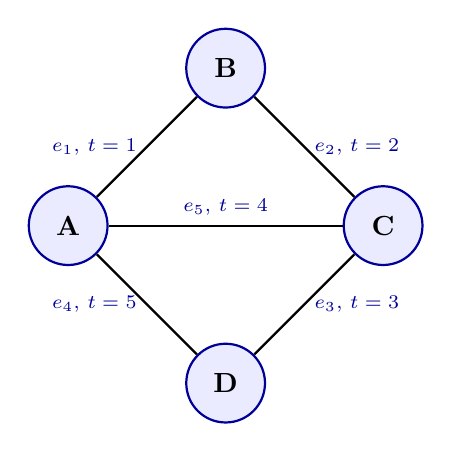
\begin{tikzpicture}[
  nd/.style={circle, draw=blue!60!black, fill=blue!8, thick,
             minimum size=10mm, font=\bfseries},
  ev/.style={font=\scriptsize, color=blue!60!black},
  >=Stealth, thick
]
% Nodes in a square
\node[nd] (A) at (0, 2)  {A};
\node[nd] (B) at (2, 4)  {B};
\node[nd] (C) at (4, 2)  {C};
\node[nd] (D) at (2, 0)  {D};

% Edges with timestamps
\draw (A) -- node[ev, left]{$e_1,\,t=1$} (B);
\draw (B) -- node[ev, right]{$e_2,\,t=2$} (C);
\draw (C) -- node[ev, right]{$e_3,\,t=3$} (D);
\draw (D) -- node[ev, left]{$e_4,\,t=5$} (A);
\draw (A) -- node[ev, above]{$e_5,\,t=4$} (C);
\end{tikzpicture}
\caption{The four-node, five-event temporal network used in the reachability comparison.
Edge labels show the event identifier and its timestamp.}
\label{fig:reachability_example}
\end{figure}

\subsection{Computing Static Reachability}

In the static projection $G = (\{A,B,C,D\}, \{\{A,B\},\{B,C\},\{C,D\},\{D,A\},\{A,C\}\})$,
we simply ask: is there any path (ignoring time) from $u$ to $v$?

Since the graph is connected (you can traverse from any node to any other), the answer is
\textbf{yes for all pairs}. The static reachability matrix $R^{\text{static}}$ where
$R^{\text{static}}_{uv} = 1$ iff $u$ can reach $v$ in $G$:

\[
R^{\text{static}} =
\begin{array}{c|cccc}
  & A & B & C & D \\
\hline
A & 1 & 1 & 1 & 1 \\
B & 1 & 1 & 1 & 1 \\
C & 1 & 1 & 1 & 1 \\
D & 1 & 1 & 1 & 1 \\
\end{array}
\]

All entries are 1: every node reaches every other node. (We include diagonal entries as 1
by convention: every node trivially reaches itself.)

\subsection{Computing Temporal Reachability}

Now we apply the strict time-ordering rule. We trace all time-respecting paths from each node.

\begin{examplebox}{Temporal Reachability: Node A}
Events involving A: $e_1$ (A--B, $t=1$), $e_5$ (A--C, $t=4$), $e_4$ (D--A, $t=5$, but this
is \textit{incoming} to A).

\textbf{From A, outgoing in time:}
\begin{itemize}[noitemsep]
  \item $e_1$: $A \xrightarrow{t=1} B$. From B: $e_2$ (B--C, $t=2>1$) $\Rightarrow B \xrightarrow{t=2} C$. From C: $e_3$ (C--D, $t=3>2$) $\Rightarrow C \xrightarrow{t=3} D$. Also $e_5$ (A--C, $t=4>2$) but we came \textit{to} C, not from A again.
  \item $e_5$: $A \xrightarrow{t=4} C$. From C: $e_3$ (C--D, $t=3$). But $3 < 4$, so this is \textbf{not} valid. No forward events from C after $t=4$.
\end{itemize}
$\mathcal{I}(A) = \{A, B, C, D\}$ (all reachable).
\end{examplebox}

\begin{examplebox}{Temporal Reachability: Node B}
Events involving B: $e_1$ (A--B, $t=1$, incoming), $e_2$ (B--C, $t=2$, outgoing).

\textbf{From B outgoing:}
$B \xrightarrow{t=2} C \xrightarrow{t=3} D$. Node D: event $e_4$ (D--A, $t=5>3$), so
$D \xrightarrow{t=5} A$. But this is an event \textit{involving} D and A; since we arrived at
D at $t=3$, and $e_4$ is at $t=5>3$, A is reachable.

Can B reach A? Only through D at $t=5$. Yes: $B \to C \to D \to A$ with times $2<3<5$.

$\mathcal{I}(B) = \{B, C, D, A\}$.
\end{examplebox}

\begin{examplebox}{Temporal Reachability: Node C}
Events involving C: $e_2$ (B--C, $t=2$), $e_3$ (C--D, $t=3$), $e_5$ (A--C, $t=4$).

\textbf{From C outgoing:}
\begin{itemize}[noitemsep]
  \item $C \xrightarrow{t=3} D$ (via $e_3$). From D: $e_4$ (D--A, $t=5>3$). So $C \to D \to A$.
  \item Event $e_5$ is at $t=4>3$ but it involves A and C. Since we are \textit{at} C after
        time $t=3$, we need events where C is the \textit{source}. $e_5$ is the contact $(A,C,4)$:
        this is A meeting C at $t=4$. If we are already at C, can we reach A via $e_5$? Yes: $C
        \xrightarrow{e_5,\,t=4} A$ (undirected contact, so C can transmit to A at $t=4$ as long
        as $4 > 3$). (\textit{Wait}: we need to check: does this make a valid path? $C$ starts at
        time $0$ (or whenever), and is involved in $e_3$ at $t=3$ and $e_5$ at $t=4$. The path
        $C \xrightarrow{t=3} D$ leads to D, not a return to C.)
\end{itemize}

Let us be systematic. From node C at the \textit{start} of the observation:
\begin{itemize}[noitemsep]
  \item Direct 1-hop: $C \xrightarrow{t=3} D$; $C \xrightarrow{t=4} A$ (via $e_5$, undirected).
  \item From D at $t=3$: $D \xrightarrow{t=5} A$ (via $e_4$). Conflict: we also reached A via $e_5$ at $t=4$.
  \item From A at $t=4$ (reached via $e_5$): no outgoing events from A after $t=4$ except $e_4$ which is \textit{incoming} to A.
\end{itemize}

Can C reach B? B only appears in $e_1$ ($t=1$) and $e_2$ ($t=2$), both \textit{before} C's
first event at $t=3$. So B is \textbf{not reachable} from C via time-respecting paths.

$\mathcal{I}(C) = \{C, D, A\}$. Note: \textbf{B is not reachable from C}!
\end{examplebox}

\begin{examplebox}{Temporal Reachability: Node D}
Events involving D: $e_3$ (C--D, $t=3$, incoming), $e_4$ (D--A, $t=5$).

\textbf{From D outgoing:} $D \xrightarrow{t=5} A$ (via $e_4$). From A at $t=5$: no later
events. From A, can we reach B or C after $t=5$? No events involve A, B, or C after $t=5$.

$\mathcal{I}(D) = \{D, A\}$. D can only reach itself and A.
\end{examplebox}

\subsection{Side-by-Side Comparison}

\begin{examplebox}{Static vs.\ Temporal Reachability Matrix}

\begin{center}
\begin{tabular}{cc}
\begin{tabular}{c|cccc}
\multicolumn{5}{c}{\textbf{Static reachability} $R^{\text{static}}$}\\[2pt]
  & A & B & C & D \\
\hline
A & 1 & 1 & 1 & 1 \\
B & 1 & 1 & 1 & 1 \\
C & 1 & 1 & 1 & 1 \\
D & 1 & 1 & 1 & 1 \\
\end{tabular}
&
\begin{tabular}{c|cccc}
\multicolumn{5}{c}{\textbf{Temporal reachability} $R^T$}\\[2pt]
  & A & B & C & D \\
\hline
A & 1 & 1 & 1 & 1 \\
B & 1 & 1 & 1 & 1 \\
C & 1 & \textcolor{red!70!black}{\textbf{0}} & 1 & 1 \\
D & 1 & \textcolor{red!70!black}{\textbf{0}} & \textcolor{red!70!black}{\textbf{0}} & 1 \\
\end{tabular}
\end{tabular}
\end{center}

\medskip
The entries marked in \textcolor{red!70!black}{\textbf{red}} are \textbf{phantom paths}: the
static graph claims $C \leadsto B$ and $D \leadsto B$ and $D \leadsto C$, but no
time-respecting path exists for these pairs.

\textbf{Explanation of each phantom:}
\begin{itemize}[noitemsep]
  \item $C \to B$: B's only events are at $t=1$ and $t=2$. C's earliest outgoing event is at
        $t=3$. No valid path from C can reach B at a time after C was first involved.
  \item $D \to B$: D's earliest outgoing event is at $t=5$. B's last event is at $t=2$. No
        path from D can travel back to $t=2$ to reach B.
  \item $D \to C$: D can only reach A (at $t=5$). From A there are no later events involving
        C.
\end{itemize}

Note also the \textbf{asymmetry}: $R^T_{AB} = 1$ (A reaches B) but $R^T_{BA} = 1$ too in
this example because the cycle A--B--C--D--A eventually loops. In general, temporal
reachability need not be symmetric even in undirected networks.
\end{examplebox}

%=============================================================================
\section{Adjacency Representation of Temporal Networks}
\label{sec:adjacency_representation}
%=============================================================================

\subsection{The Adjacency Tensor $\mathbf{A}(t)$}

For a static graph we use the \textbf{adjacency matrix} $A \in \{0,1\}^{n \times n}$, where
$A_{ij} = 1$ iff there is an edge between $i$ and $j$. For a temporal network, we need to
capture the time dimension as well.

\begin{conceptbox}{The Adjacency Tensor}
Define $A_{ij}(t) = 1$ if nodes $i$ and $j$ were in contact at time $t$, and $A_{ij}(t) = 0$
otherwise. This gives a function $\mathbf{A} : \mathcal{T} \to \{0,1\}^{n \times n}$, which
we can think of as a \textbf{three-dimensional tensor} (a cube of numbers) with dimensions:
\[
  \underbrace{n}_{\text{node }i} \times \underbrace{n}_{\text{node }j} \times
  \underbrace{T}_{\text{time slice }t}
\]
For each time step $t$, the slice $\mathbf{A}(\cdot, \cdot, t) = A_t$ is the adjacency matrix
of the \textbf{snapshot graph} at time $t$.

For \textbf{instantaneous contacts} (our case), $A_{ij}(t) = 1$ only at isolated time points.
For \textbf{discrete time}, $t$ takes integer values and we can write $\mathbf{A}$ as a stack
of $T$ binary matrices of size $n \times n$.
\end{conceptbox}

\begin{examplebox}{Adjacency Tensor for the Four-Node Example}
Using the events $\{(A,B,1), (B,C,2), (C,D,3), (A,C,4), (D,A,5)\}$ and discrete time steps
$t \in \{1,2,3,4,5\}$:

\medskip
\noindent$A_1$ (contacts at $t=1$): only $A$--$B$.
\[
A_1 = \begin{pmatrix} 0&1&0&0\\ 1&0&0&0\\ 0&0&0&0\\ 0&0&0&0 \end{pmatrix}
\]

\noindent$A_2$ (contacts at $t=2$): only $B$--$C$.
\[
A_2 = \begin{pmatrix} 0&0&0&0\\ 0&0&1&0\\ 0&1&0&0\\ 0&0&0&0 \end{pmatrix}
\]
And so on for $t=3,4,5$. At all other time steps (and all steps not listed), $A_t = \mathbf{0}$.
\end{examplebox}

\subsection{The COO Format: How Computers Store Sparse Temporal Graphs}

The adjacency tensor is very sparse: most entries are zero (most pairs of nodes are not in
contact at any given moment). Storing the full $n \times n \times T$ tensor wastes enormous
amounts of memory. Instead, computers use the \textbf{coordinate (COO) format}: store only the
non-zero entries as a list of (row, column, value) triples.

For a temporal network, the COO format stores each event $(u, v, t)$ explicitly. This is
exactly the event list we have been using all along.

\begin{conceptbox}{COO Format for Temporal Networks}
The COO event list for a temporal network with $|E^T|$ events is:
\[
\underbrace{\begin{pmatrix} u_1 \\ v_1 \\ t_1 \end{pmatrix},\;
\begin{pmatrix} u_2 \\ v_2 \\ t_2 \end{pmatrix},\;
\ldots,\;
\begin{pmatrix} u_{|E^T|} \\ v_{|E^T|} \\ t_{|E^T|} \end{pmatrix}}_{\text{one column per event}}
\]
This is stored as a matrix with 3 rows and $|E^T|$ columns.

In \textbf{PyTorch Geometric} (the GNN library used in this project), the graph connectivity is
stored in \texttt{edge\_index}: a $2 \times |E|$ tensor where the first row contains source
node indices and the second row contains target node indices. Edge features (including
timestamps) are stored separately in \texttt{edge\_attr}.
\end{conceptbox}

\begin{examplebox}{From Event List to PyTorch Geometric Format}
Our four-node example has events (using integer node labels $0=A, 1=B, 2=C, 3=D$):
\begin{itemize}[noitemsep]
  \item $(A,B,1) \to (0,1,1)$
  \item $(B,C,2) \to (1,2,2)$
  \item $(C,D,3) \to (2,3,3)$
  \item $(A,C,4) \to (0,2,4)$
  \item $(D,A,5) \to (3,0,5)$
\end{itemize}

The PyTorch Geometric \texttt{edge\_index} for the static projection (both directions, since
undirected):
\[
\texttt{edge\_index} = \begin{pmatrix}
0 & 1 & 1 & 2 & 2 & 3 & 0 & 3 \\
1 & 0 & 2 & 1 & 3 & 2 & 2 & 0
\end{pmatrix}
\]
(first row: sources; second row: targets; both directions included for each undirected edge).

The timestamps become \texttt{edge\_attr}:
\[
\texttt{edge\_attr} = [1,\; 1,\; 2,\; 2,\; 3,\; 3,\; 4,\; 5]
\]
corresponding to the edges in the same column order. This is exactly the format read by our
\texttt{gnn/static\_gnn.py} and temporal GNN models.
\end{examplebox}

%=============================================================================
\section{Temporal Centrality Metrics}
\label{sec:temporal_centrality}
%=============================================================================

Classical centrality metrics like degree, betweenness, and closeness have \textit{temporal}
counterparts that carry substantially more epidemiological information. We define each one,
give intuition, and then compute it step by step on our running example.

\subsection{Temporal Degree}

\begin{conceptbox}{Temporal Degree: Definition}
The \textbf{temporal degree} of node $v$ is the total number of events (contacts) involving
$v$ in the observation window:
\[
  k_v^T = \bigl|\{(u, v, t) \in E^T\}\bigr| + \bigl|\{(v, w, t) \in E^T\}\bigr|
\]
In plain English: count every event where $v$ appears on either side.

This differs from the \textbf{static degree} $k_v = |\mathcal{N}(v)|$, which counts the
number of \textit{distinct neighbours} of $v$. A node with many repeated contacts to the same
neighbour has high temporal degree but the same static degree as a node with one contact to
that neighbour.
\end{conceptbox}

\begin{examplebox}{Computing Temporal Degree for All Four Nodes}
Event list: $\{(A,B,1), (B,C,2), (C,D,3), (A,C,4), (D,A,5)\}$.

\begin{center}
\begin{tabular}{lll}
\toprule
\textbf{Node} & \textbf{Events involving this node} & \textbf{Temporal degree $k_v^T$} \\
\midrule
A & $(A,B,1)$, $(A,C,4)$, $(D,A,5)$ & 3 \\
B & $(A,B,1)$, $(B,C,2)$             & 2 \\
C & $(B,C,2)$, $(C,D,3)$, $(A,C,4)$ & 3 \\
D & $(C,D,3)$, $(D,A,5)$             & 2 \\
\bottomrule
\end{tabular}
\end{center}

Static degrees: A has 3 neighbours ($B,C,D$), B has 2, C has 3, D has 2. In this particular
example the numbers match because no node has repeated contacts with the same neighbour.

\textbf{What can temporal degree tell us?} High temporal degree means a node is frequently
involved in contacts. In an epidemic context, a node with many events is likely to be infected
early and to transmit widely. But temporal degree alone does not capture \textit{when} those
events occur or whether they can form valid transmission chains.
\end{examplebox}

\subsection{Temporal Betweenness Centrality}

\begin{conceptbox}{Temporal Betweenness: Definition}
The \textbf{temporal betweenness centrality} of node $v$ measures how often $v$ lies on the
\textit{fastest} (shortest hop count) time-respecting paths between all other pairs of nodes:
\[
  C_B^T(v) = \sum_{\substack{s \neq v \neq d \\ s,d \in \mathcal{V}}}
             \frac{\sigma^T(s, d \mid v)}{\sigma^T(s, d)}
\]
where:
\begin{itemize}[noitemsep]
  \item $\sigma^T(s, d)$ --- the number of shortest (minimum-hop) time-respecting paths from
        $s$ to $d$.
  \item $\sigma^T(s, d \mid v)$ --- the number of those shortest paths that pass through $v$.
  \item The fraction $\sigma^T(s, d \mid v) / \sigma^T(s, d)$ is the proportion of shortest
        paths through $v$ for the pair $(s, d)$.
\end{itemize}
Summing over all ordered pairs $(s, d)$ with $s \neq v \neq d$ gives the total centrality.
\end{conceptbox}

\begin{examplebox}{Temporal Betweenness: Step-by-Step for Four Nodes}
We use strict time-ordering and unit edge weights (hop count). We already know the
time-respecting paths, so we identify the \textit{shortest} (fewest hops) ones for each pair.

\medskip
\noindent\textbf{All ordered pairs and their shortest time-respecting paths:}

\begin{center}
\begin{tabular}{llll}
\toprule
$(s,d)$ & Shortest temporal path(s) & Hops & Intermediaries \\
\midrule
$(A,B)$ & $A \xrightarrow{1} B$ & 1 & none \\
$(A,C)$ & $A \xrightarrow{4} C$ and $A \xrightarrow{1} B \xrightarrow{2} C$ & 1 and 2 & shortest: none (direct hop) \\
$(A,D)$ & $A \xrightarrow{1} B \xrightarrow{2} C \xrightarrow{3} D$ and $A \xrightarrow{4} C \xrightarrow{?}$ (no later C--D event after $t=4$) & 3 & B, C \\
$(B,C)$ & $B \xrightarrow{2} C$ & 1 & none \\
$(B,D)$ & $B \xrightarrow{2} C \xrightarrow{3} D$ & 2 & C \\
$(B,A)$ & $B \xrightarrow{2} C \xrightarrow{3} D \xrightarrow{5} A$ & 3 & C, D \\
$(C,D)$ & $C \xrightarrow{3} D$ & 1 & none \\
$(C,A)$ & $C \xrightarrow{4} A$ and $C \xrightarrow{3} D \xrightarrow{5} A$ & 1 and 2 & shortest: none (direct hop) \\
$(D,A)$ & $D \xrightarrow{5} A$ & 1 & none \\
$(C,B)$ & \textbf{none} (phantom) & --- & --- \\
$(D,B)$ & \textbf{none} (phantom) & --- & --- \\
$(D,C)$ & \textbf{none} (phantom) & --- & --- \\
\bottomrule
\end{tabular}
\end{center}

\medskip
\noindent\textbf{Counting betweenness contributions:}

For each node $v$, sum over all pairs $(s,d)$ the fraction of shortest temporal paths through
$v$:

\begin{itemize}
  \item \textbf{Node B:}
    \begin{itemize}[noitemsep]
      \item $(A,D)$: shortest path is $A \to B \to C \to D$ (3 hops). B is on this path.
            Contribution: $1/1 = 1$.
      \item $(B,A)$: B is the source, not an intermediary. Not counted.
      \item No other shortest paths pass through B.
    \end{itemize}
    $C_B^T(B) = 1$.

  \item \textbf{Node C:}
    \begin{itemize}[noitemsep]
      \item $(A,D)$: $A \to B \to C \to D$. C is on this path. Contribution: $1/1 = 1$.
      \item $(B,D)$: $B \to C \to D$. C is on this path. Contribution: $1/1 = 1$.
      \item $(B,A)$: $B \to C \to D \to A$. C is on this path. Contribution: $1/1 = 1$.
    \end{itemize}
    $C_B^T(C) = 3$.

  \item \textbf{Node D:}
    \begin{itemize}[noitemsep]
      \item $(B,A)$: $B \to C \to D \to A$. D is on this path. Contribution: $1/1 = 1$.
    \end{itemize}
    $C_B^T(D) = 1$.

  \item \textbf{Node A:} We check all pairs where A is neither source nor destination:
    \begin{itemize}[noitemsep]
      \item $(B,C)$: $B \to C$ directly. A not involved.
      \item $(B,D)$: $B \to C \to D$. A not involved.
      \item $(C,D)$: $C \to D$ directly. A not involved.
      \item $(D,A)$: D is source, A is destination.
    \end{itemize}
    $C_B^T(A) = 0$.
\end{itemize}

\medskip
\noindent\textbf{Summary:}
\begin{center}
\begin{tabular}{cc}
\toprule
\textbf{Node} & \textbf{Temporal betweenness $C_B^T(v)$} \\
\midrule
A & 0 \\
B & 1 \\
C & \textbf{3} \\
D & 1 \\
\bottomrule
\end{tabular}
\end{center}
\end{examplebox}

\begin{keyinsight}{Static vs.\ Temporal Centrality Can Disagree Strongly}
In the static graph, all nodes have the same degree (A: 3, B: 2, C: 3, D: 2) and the static
betweenness of each node is influenced by the number of shortest static paths passing through
it. In this connected, roughly symmetric graph, static betweenness would distribute roughly
evenly.

The temporal betweenness, however, concentrates on node \textbf{C}: C is on 3 out of 4 pairs
that have temporal paths through an intermediary. This is because C is in the ``middle'' of
the time ordering: it is reachable early (at $t=2$ from B, at $t=3$ from the chain starting
at A) and has outgoing temporal contacts later.

\textbf{Epidemiological consequence:} If we were looking for the most important superspreader
in this network --- the node that, if removed, would most reduce temporal spread --- temporal
betweenness tells us it is C, not the high-static-degree nodes A or C (which happen to tie).
A static betweenness calculation might rank A higher because of its three static neighbours,
but temporal analysis correctly identifies C as the temporal hub.
\end{keyinsight}

%=============================================================================
\section{Inter-Event Time Distributions and Burstiness}
\label{sec:interevent_times}
%=============================================================================

\subsection{What is an Inter-Event Time?}

Consider a single node $v$ that participates in a series of contacts at times
$t_1 < t_2 < t_3 < \cdots < t_m$. The \textbf{inter-event times} are the gaps between
consecutive contacts:
\[
  \tau_1 = t_2 - t_1, \quad \tau_2 = t_3 - t_2, \quad \ldots, \quad \tau_{m-1} = t_m - t_{m-1}.
\]
Each $\tau_i$ is a positive number representing how long node $v$ waited between one contact
and the next.

\subsection{Poisson vs.\ Bursty Contact Patterns}

\begin{analogybox}{Bus Arrivals: Regular vs.\ Bursty}
Imagine waiting at a bus stop. In the ideal world, buses arrive exactly every 10 minutes:
perfectly \textbf{regular} (periodic). In a less ideal world, buses come at random but with an
average of one every 10 minutes: a \textbf{Poisson process}. In the real world, buses sometimes
cluster: three come in a row (a ``burst''), then nothing for 40 minutes.

The third pattern is called \textbf{bursty}: long silences punctuated by intense bursts of
activity. This is precisely what contact data looks like in real epidemiological settings.
Hospital staff talk intensely during morning rounds (a burst), then have long gaps during
administrative hours. The same pattern appears in phone calls, email, and face-to-face contact
sensors.

\textbf{Why does burstiness matter for epidemics?} Consider two nodes, each with an average
of 1 contact per hour:
\begin{itemize}[noitemsep]
  \item \textbf{Regular node}: contacts every hour, on the clock.
  \item \textbf{Bursty node}: 5 contacts within a 10-minute window, then silence for 5 hours.
\end{itemize}
The bursty node has long silent periods during which a pathogen it is carrying would cause
recovery before transmission. In the short burst windows, it transmits rapidly. The net effect
is often \textit{slower} epidemic spread than the regular node, despite the same average rate.
\end{analogybox}

\begin{figure}[H]
\centering
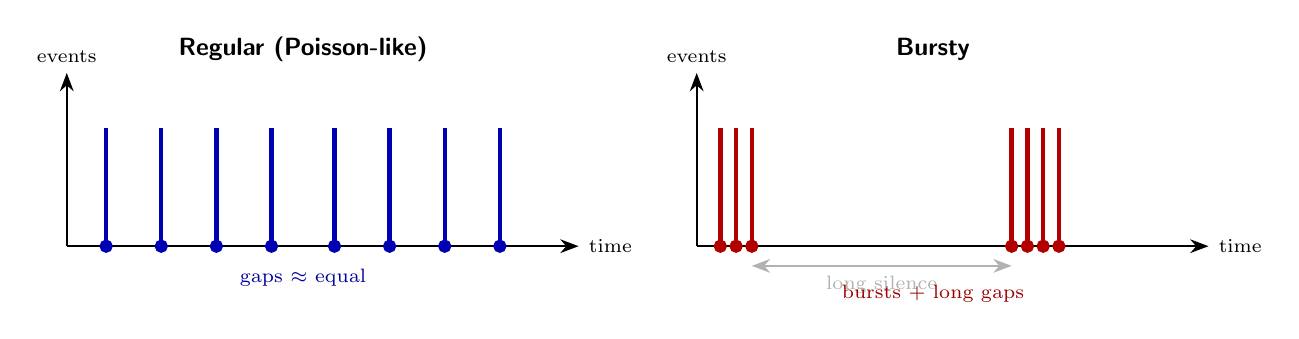
\begin{tikzpicture}[
  >=Stealth, thick,
  label/.style={font=\small\bfseries\sffamily}
]
% Left panel: regular (Poisson-like) contact sequence
\begin{scope}[xshift=0cm]
  \node[label] at (3, 2.5) {Regular (Poisson-like)};
  \draw[->] (0,0) -- (6.5,0) node[right,font=\scriptsize]{time};
  \draw[->] (0,0) -- (0,2.2) node[above,font=\scriptsize]{events};
  % Bars at roughly equal spacing
  \foreach \x in {0.5, 1.2, 1.9, 2.6, 3.4, 4.1, 4.8, 5.5}{
    \draw[blue!70!black, ultra thick] (\x,0) -- (\x,1.5);
    \filldraw[blue!70!black] (\x,0) circle (2pt);
  }
  \node[font=\scriptsize, color=blue!60!black] at (3, -0.4) {gaps $\approx$ equal};
\end{scope}

% Right panel: bursty contact sequence
\begin{scope}[xshift=8cm]
  \node[label] at (3, 2.5) {Bursty};
  \draw[->] (0,0) -- (6.5,0) node[right,font=\scriptsize]{time};
  \draw[->] (0,0) -- (0,2.2) node[above,font=\scriptsize]{events};
  % Burst 1: three close events
  \foreach \x in {0.3, 0.5, 0.7}{
    \draw[red!70!black, ultra thick] (\x,0) -- (\x,1.5);
    \filldraw[red!70!black] (\x,0) circle (2pt);
  }
  % Long gap then Burst 2
  \foreach \x in {4.0, 4.2, 4.4, 4.6}{
    \draw[red!70!black, ultra thick] (\x,0) -- (\x,1.5);
    \filldraw[red!70!black] (\x,0) circle (2pt);
  }
  % Annotation for gap
  \draw[<->, gray!60, thick] (0.7, -0.25) -- node[below,font=\scriptsize]{long silence} (4.0, -0.25);
  \node[font=\scriptsize, color=red!60!black] at (3, -0.6) {bursts + long gaps};
\end{scope}
\end{tikzpicture}
\caption{Comparison of a regular (Poisson-like) contact sequence (left) and a bursty contact
sequence (right). The bursty sequence has the same number of events but concentrates them in
short bursts separated by long silences. This pattern is ubiquitous in real contact data
(hospital wards, phone logs, proximity sensors) and has significant consequences for epidemic
dynamics.}
\label{fig:burstiness}
\end{figure}

\subsection{Quantifying Burstiness: The $B$ Parameter}

\begin{mathbox}{The Burstiness Parameter}
Let $\mu_\tau = \mathbb{E}[\tau]$ be the \textbf{mean} inter-event time and $\sigma_\tau =
\sqrt{\mathrm{Var}[\tau]}$ be the \textbf{standard deviation} of inter-event times for a node.
The \textbf{burstiness parameter} is:
\[
  B = \frac{\sigma_\tau - \mu_\tau}{\sigma_\tau + \mu_\tau} \in (-1,\, 1).
\]

\textbf{Interpreting the three limiting cases:}
\begin{itemize}
  \item \textbf{Perfectly periodic} ($\sigma_\tau = 0$): all gaps are equal, $\sigma_\tau = 0$.
        Then $B = (0 - \mu_\tau)/(0 + \mu_\tau) = -1$. Maximum negative burstiness: completely
        regular activity.
  \item \textbf{Poisson process} ($\tau \sim \text{Exp}(\lambda)$): for an exponential
        distribution, the mean equals the standard deviation, $\sigma_\tau = \mu_\tau$. Then
        $B = 0$. Neutral: random but not particularly bursty.
  \item \textbf{Maximally bursty} ($\sigma_\tau \gg \mu_\tau$): a few very large gaps dominate,
        so $\sigma_\tau \to \infty$ relative to $\mu_\tau$. Then $B \to 1$. Maximum positive
        burstiness: intense bursts separated by very long silences.
\end{itemize}

\textbf{Empirical finding:} Real human contact networks typically have $B \in [0.2, 0.8]$,
indicating moderately bursty activity. This is why epidemic simulation cannot simply assume
Poisson contacts.
\end{mathbox}

\begin{examplebox}{Computing Burstiness for a Node}
Suppose node $v$ has contacts at times $t = \{1, 2, 3, 10, 11, 12\}$. The inter-event times
are:
\[
  \tau = \{t_2 - t_1,\, t_3 - t_2,\, t_4 - t_3,\, t_5 - t_4,\, t_6 - t_5\}
       = \{1, 1, 7, 1, 1\}.
\]

\textbf{Mean:}
\[
  \mu_\tau = \frac{1 + 1 + 7 + 1 + 1}{5} = \frac{11}{5} = 2.2
\]

\textbf{Standard deviation:}
\[
  \sigma_\tau = \sqrt{\frac{(1-2.2)^2 + (1-2.2)^2 + (7-2.2)^2 + (1-2.2)^2 + (1-2.2)^2}{5}}
\]
\[
  = \sqrt{\frac{1.44 + 1.44 + 23.04 + 1.44 + 1.44}{5}}
  = \sqrt{\frac{28.8}{5}} = \sqrt{5.76} = 2.4
\]

\textbf{Burstiness:}
\[
  B = \frac{2.4 - 2.2}{2.4 + 2.2} = \frac{0.2}{4.6} \approx 0.043
\]

This is nearly Poisson ($B \approx 0$). Intuitively: although we see two ``bursts'' of
contacts, the single large gap ($\tau_3 = 7$) is only $3\times$ the mean gap. True bursty
sequences have gaps that are $10$--$100\times$ the mean.

\textbf{Compare with a truly bursty node} whose inter-event times are $\{0.1, 0.1, 0.1, 50,
0.1\}$:
\[
  \mu_\tau = \frac{50.4}{5} = 10.08, \quad
  \sigma_\tau \approx 19.9, \quad
  B = \frac{19.9 - 10.08}{19.9 + 10.08} \approx 0.33.
\]
This is moderately bursty ($B \approx 0.33$), reflecting the one long gap of 50 time units
surrounded by rapid-fire contacts.
\end{examplebox}

\begin{keyinsight}{Burstiness and Source Detection}
A node that is bursty may look less infectious than its average contact rate suggests: its
long silent periods give the pathogen time to ``time out'' (the $\Delta t$ constraint). When
fitting epidemic models or choosing the $\Delta t$ parameter in a $\Delta t$-constrained path
analysis, bursty contact distributions require special attention. Incorrectly assuming Poisson
contacts in a bursty network will lead to wrong reachability estimates and, consequently, wrong
source predictions.
\end{keyinsight}

%=============================================================================
\section{How the Codebase Represents Temporal Networks}
\label{sec:codebase_representation}
%=============================================================================

Having built the theory from scratch, we now close the loop by showing exactly how these
concepts are implemented in the project codebase. Every abstract object introduced in this
chapter has a concrete counterpart in the code.

\subsection{The Event List Format}

The project stores temporal networks as a list of $(u, v, t)$ triples, sorted by time. This is
the COO format described in Section~\ref{sec:adjacency_representation}. In Python, after
loading via NetworkX, the function \texttt{make\_array\_from\_networkx} (in
\texttt{setup/read\_network.py}) converts the graph object to a plain NumPy array:

\begin{codewalk}{make\_array\_from\_networkx in setup/read\_network.py}
\begin{lstlisting}[language=Python]
def make_array_from_networkx(H):
    """From the networkx graph, make a numpy array
    with rows (u, v, t), sorted by t."""
    rows = []
    for u, v, data in H.edges(data=True):
        # Each edge stores a list of timestamps
        rows.extend([[u, v, t] for t in data['times']])
    arr = np.array(rows)
    arr = arr[arr[:, 2].argsort()]  # sort by time
    return arr
\end{lstlisting}

The result is a NumPy array with shape \texttt{(|E\^{}T|, 3)}, where:
\begin{itemize}[noitemsep]
  \item Column 0: source node $u$ (integer index)
  \item Column 1: target node $v$ (integer index)
  \item Column 2: timestamp $t$
\end{itemize}

For an Alice--Bob--Carol style example, this would look like:
\begin{lstlisting}[language=Python]
# arr for a 3-node, 3-event network:
arr = np.array([
    [0, 1, 1],   # Alice(0) -- Bob(1)   at t=1
    [1, 2, 2],   # Bob(1)   -- Carol(2) at t=2
    [2, 0, 7],   # Carol(2) -- Alice(0) at t=7
])
\end{lstlisting}
\end{codewalk}

\subsection{Loading the Network}

The entry point for loading a temporal network is \texttt{setup/read\_network.py}. It handles
two cases:

\begin{codewalk}{load\_network in setup/read\_network.py}
\begin{lstlisting}[language=Python]
def load_network(cfg, label_attribute="old_id"):
    if cfg.nwk.type == "empirical":
        # Load from CSV file: each row is "u v t"
        H = read_networkx(
            'nwk/' + cfg.nwk.name + '.csv',
            t_max=cfg.nwk.t_max,
            directed=cfg.nwk.directed
        )
    elif cfg.nwk.type == "synthetic":
        # Generate e.g. Erdos-Renyi with all time steps
        H = generate_synthetic_graph(cfg)
    return H
\end{lstlisting}

For \textbf{empirical networks}, each line of the CSV file contains \texttt{u v t}: the two
node labels and the timestamp. Events after \texttt{t\_max} are ignored. Self-contacts
(where $u = v$) are discarded. The function returns a NetworkX graph object where each edge
\texttt{(u, v)} carries a \texttt{'times'} attribute: a list of all timestamps at which that
pair was in contact.

For \textbf{synthetic networks} (e.g.\ Erd\H{o}s--R\'enyi graphs), the contact times are set
to \texttt{range(t\_max + 1)}: every edge is active at every discrete time step. This is the
``always-on'' baseline that is equivalent to a static graph for temporal methods.
\end{codewalk}

\subsection{The TSIRData Dataclass}

Once simulations have been run, all data --- network, simulation outcomes, and ground truth ---
is stored in a single \texttt{TSIRData} dataclass (in \texttt{setup/data\_loader.py}):

\begin{codewalk}{TSIRData Dataclass in setup/data\_loader.py}
\begin{lstlisting}[language=Python]
@dataclass
class TSIRData:
    config: dict         # experiment configuration
    n_nodes: int         # |V|: number of nodes
    n_runs: int          # ground-truth simulation runs
    mc_runs: int         # Monte Carlo simulation runs
    # Monte Carlo SIR state arrays, shape: (n_nodes, mc_runs, n_nodes)
    mc_S: np.ndarray     # mc_S[s, r, v] = 1 if node v is Susceptible
    mc_I: np.ndarray     #   in run r of MC sim starting at source s
    mc_R: np.ndarray
    # Ground truth SIR state arrays, shape: (n_nodes, n_runs, n_nodes)
    truth_S: np.ndarray  # truth_S[s, r, v] = 1 if node v is Susceptible
    truth_I: np.ndarray  #   in ground-truth run r with true source s
    truth_R: np.ndarray
    # Binary masks for filtering:
    maximal_outbreak: np.ndarray  # shape (n_nodes, n_nodes)
    possible: np.ndarray          # shape (n_nodes, n_runs, n_nodes)
    lik_possible: np.ndarray      # log-likelihood correction mask
\end{lstlisting}

The three-dimensional arrays deserve explanation:
\begin{itemize}
  \item \texttt{truth\_S[s, r, v]}: the SIR state of node $v$ in run $r$ of the ground-truth
        simulation, given that node $s$ was the true source. This is the label data our GNN
        trains on.
  \item \texttt{mc\_S[s, r, v]}: the SIR state of node $v$ in Monte Carlo run $r$ with
        seed node $s$. These are the simulated ``observations'' the model uses for inference.
  \item \texttt{maximal\_outbreak[s, v]}: 1 if node $v$ \textit{ever} becomes infected in any
        run with source $s$, 0 otherwise. This is exactly the temporal reachability indicator
        $\mathbf{1}[s \leadsto v]$ --- a direct implementation of the temporal reachability
        concept from Section~\ref{sec:reachability_comparison}.
\end{itemize}
\end{codewalk}

\begin{keyinsight}{Theory Meets Code}
Every concept in this chapter has a direct counterpart in the codebase:
\begin{itemize}[noitemsep]
  \item The event list $(u, v, t)$ $\Leftrightarrow$ the \texttt{arr} array from
        \texttt{make\_array\_from\_networkx}.
  \item The observation window $\mathcal{T}$ $\Leftrightarrow$ \texttt{cfg.nwk.t\_max}.
  \item The $\Delta t$ constraint $\Leftrightarrow$ the SIR parameter \texttt{cfg.sir.mu}
        (recovery rate; $\Delta t \approx 1/\mu$).
  \item Temporal reachability $\mathcal{I}(s)$ $\Leftrightarrow$
        \texttt{TSIRData.maximal\_outbreak[s, :]}.
  \item The static projection $G$ $\Leftrightarrow$ the NetworkX graph $H$ (which stores the
        edge list but ignores timing when passed to a static GNN).
\end{itemize}
The entire research project is, at its core, an attempt to exploit the temporal information
that the static projection discards --- to use $E^T$ instead of $G$ whenever possible.
\end{keyinsight}

%=============================================================================
\section{Static Projection and Information Loss}
\label{sec:static_projection}
%=============================================================================

We formalise what we lose when we project a temporal network to a static graph.

\begin{mathbox}{The Static Projection: Formal Definition}
Given a temporal network $G^T = (\mathcal{V}, E^T, \mathcal{T})$, its \textbf{static
projection} is the undirected graph $G = (\mathcal{V}, \mathcal{E})$ where:
\[
  (u, v) \in \mathcal{E} \iff \exists\, t \in \mathcal{T} : (u, v, t) \in E^T.
\]
In words: two nodes are connected in $G$ if and only if they were in contact at
\textit{any} point during the observation window.
\end{mathbox}

\begin{figure}[H]
\centering
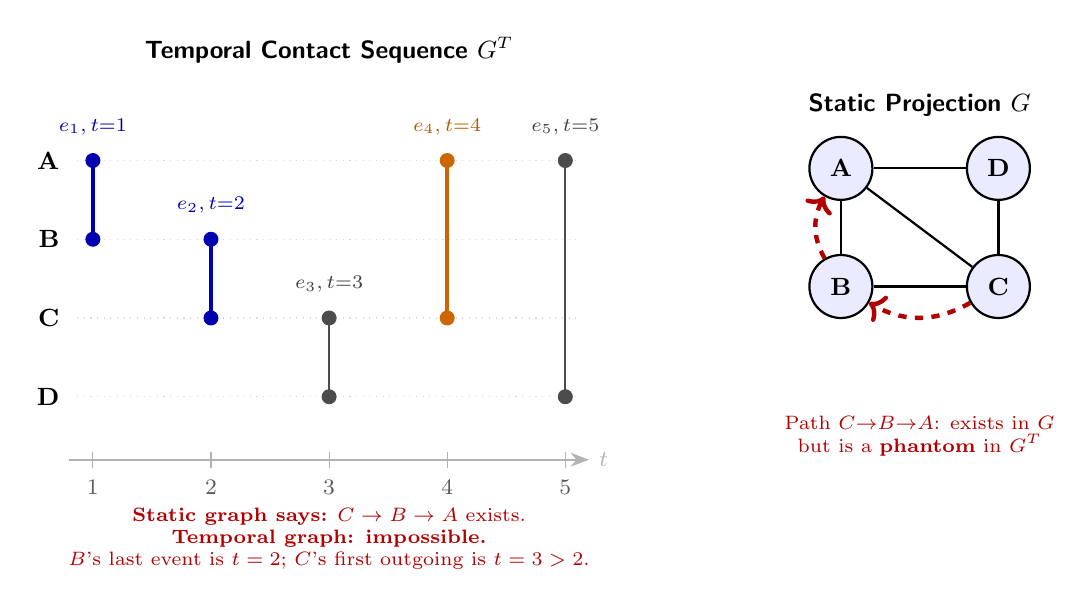
\begin{tikzpicture}[
    every node/.style={font=\small},
    event/.style={circle, draw, thick, fill=white, minimum size=8mm,
                  font=\small\bfseries},
    timelabel/.style={font=\footnotesize, color=gray!70!black},
    evtarrow/.style={-{Stealth[length=2.5mm]}, thick},
    tstamp/.style={above, font=\scriptsize, color=blue!60!black},
    projlabel/.style={font=\small\sffamily\bfseries},
]

% -------- LEFT: Temporal Network --------
\begin{scope}[xshift=0cm]
  \node[projlabel] at (3.0, 5.0) {Temporal Contact Sequence $G^T$};

  % Time axis
  \draw[-{Stealth}, thick, gray!60] (-0.3, -0.2) -- (6.3, -0.2)
        node[right, font=\footnotesize]{$t$};
  \foreach \x/\lab in {0/1, 1.5/2, 3.0/3, 4.5/4, 6.0/5}{
    \draw[gray!60] (\x, -0.1) -- (\x, -0.3);
    \node[timelabel] at (\x, -0.55) {\lab};
  }

  % Nodes on y-axis
  \foreach \y/\lbl in {0.6/D, 1.6/C, 2.6/B, 3.6/A}{
    \node[left, font=\small\bfseries] at (-0.3, \y) {\lbl};
    \draw[dotted, gray!30] (-0.2, \y) -- (6.2, \y);
  }

  % Events as vertical bars
  % e1: A-B at t=1
  \draw[blue!70!black, ultra thick] (0, 2.6) -- (0, 3.6);
  \filldraw[blue!70!black] (0,2.6) circle (2.5pt);
  \filldraw[blue!70!black] (0,3.6) circle (2.5pt);
  \node[tstamp, color=blue!70!black] at (0.0, 3.8) {$e_1,t{=}1$};

  % e2: B-C at t=2
  \draw[blue!70!black, ultra thick] (1.5, 1.6) -- (1.5, 2.6);
  \filldraw[blue!70!black] (1.5,1.6) circle (2.5pt);
  \filldraw[blue!70!black] (1.5,2.6) circle (2.5pt);
  \node[tstamp, color=blue!70!black] at (1.5, 2.8) {$e_2,t{=}2$};

  % e3: C-D at t=3
  \draw[gray!60!black, thick] (3.0, 0.6) -- (3.0, 1.6);
  \filldraw[gray!60!black] (3.0,0.6) circle (2.5pt);
  \filldraw[gray!60!black] (3.0,1.6) circle (2.5pt);
  \node[tstamp, color=gray!50!black] at (3.0, 1.8) {$e_3,t{=}3$};

  % e4: A-C at t=4  (this is the "phantom builder" in static graph)
  \draw[orange!80!black, ultra thick] (4.5, 1.6) -- (4.5, 3.6);
  \filldraw[orange!80!black] (4.5,1.6) circle (2.5pt);
  \filldraw[orange!80!black] (4.5,3.6) circle (2.5pt);
  \node[tstamp, color=orange!70!black] at (4.5, 3.8) {$e_4,t{=}4$};

  % e5: D-A at t=5
  \draw[gray!60!black, thick] (6.0, 0.6) -- (6.0, 3.6);
  \filldraw[gray!60!black] (6.0,0.6) circle (2.5pt);
  \filldraw[gray!60!black] (6.0,3.6) circle (2.5pt);
  \node[tstamp, color=gray!50!black] at (6.0, 3.8) {$e_5,t{=}5$};

  % Phantom path annotation
  \node[red!70!black, font=\scriptsize, align=center] at (3.0, -1.2)
    {\textbf{Static graph says:} $C \to B \to A$ exists.\\
     \textbf{Temporal graph: impossible.}\\
     $B$'s last event is $t=2$; $C$'s first outgoing is $t=3>2$.};
\end{scope}

% -------- RIGHT: Static Projection --------
\begin{scope}[xshift=9.5cm, yshift=0.5cm]
  \node[projlabel] at (1.0, 3.8) {Static Projection $G$};

  \node[event, fill=blue!8]   (A) at (0.0, 3.0) {A};
  \node[event, fill=blue!8]   (B) at (0.0, 1.5) {B};
  \node[event, fill=blue!8]   (C) at (2.0, 1.5) {C};
  \node[event, fill=blue!8]   (D) at (2.0, 3.0) {D};

  \draw[thick] (A)--(B);
  \draw[thick] (B)--(C);
  \draw[thick] (C)--(D);
  \draw[thick] (A)--(C);
  \draw[thick] (D)--(A);

  % Highlight the phantom path C->B->A
  \draw[red!70!black, ultra thick, dashed, ->, bend left=30]
    (C) to (B);
  \draw[red!70!black, ultra thick, dashed, ->, bend left=30]
    (B) to (A);

  \node[red!70!black, font=\scriptsize, align=center] at (1.0, -0.4)
    {Path $C{\to}B{\to}A$: exists in $G$\\but is a \textbf{phantom} in $G^T$};
\end{scope}

\end{tikzpicture}
\caption{Left: a temporal contact sequence on four nodes with five events. Nodes are arranged
on the $y$-axis; time runs left to right. The blue and orange events form valid forward paths.
Right: the static projection retains all edges but loses timestamps, creating the phantom path
$C \to B \to A$ (dashed red) which is causally impossible because B's last event ($t=2$)
precedes C's first outgoing event ($t=3$).}
\label{fig:static_projection}
\end{figure}

\begin{keyinsight}{Quantifying Information Loss}
Let $\mathcal{R}^T(u)$ denote the \textbf{temporal reachability set} of node $u$ and
$\mathcal{R}(u)$ its static reachability set. By construction $\mathcal{R}^T(u) \subseteq
\mathcal{R}(u)$ always holds. In empirical contact networks with strong burstiness, the ratio
$|\mathcal{R}^T(u)| / |\mathcal{R}(u)|$ can be as low as $0.1$--$0.3$: the static graph
over-estimates causal reach by a factor of 3--10. For source detection, this means the static
graph floods the posterior over sources with false candidates; a static GNN may assign high
probability to nodes that could never have initiated the observed outbreak.
\end{keyinsight}

\begin{analogybox}{Collapsing a Train Timetable to a Route Map}
A train timetable tells you that Train 42 leaves Munich at 08:15 and arrives Augsburg at 08:52,
while Train 7 leaves Augsburg at 08:40 for Nuremberg. The route map shows
Munich--Augsburg--Nuremberg as a connected path. But the timetable reveals the connection is
impossible: you arrive at 08:52 and your connection left at 08:40.

Collapsing a temporal network into a static graph is exactly like reducing the timetable to a
route map: you preserve topology but destroy the information needed to reason about what is
actually reachable.
\end{analogybox}

%=============================================================================
\section{The Temporal Event Graph: A Forward Pointer}
\label{sec:event_graph_pointer}
%=============================================================================

All of the path and reachability concepts developed in this chapter reach their most
computationally powerful form in the \textbf{Temporal Event Graph (TEG)} representation due
to Saram\"{a}ki, Kivel\"{a}, and Karsai. Rather than treating nodes as primary objects, the
TEG elevates \textit{events} to nodes in a static directed acyclic graph (DAG), where directed
edges encode the possibility of transmission between consecutive contacts.

\begin{keyinsight}{Why the TEG Matters for GNN-Based Source Detection}
Every concept in this chapter maps cleanly onto the TEG structure:
\begin{itemize}[noitemsep]
  \item \textbf{Time-respecting paths} in $G^T$ become \textbf{directed paths} in the TEG.
  \item \textbf{$\Delta t$-constrained paths} correspond to edges with inter-event gap
        $\leq \Delta t$ in the TEG.
  \item \textbf{Temporal reachability} corresponds to graph reachability in the DAG.
  \item \textbf{Asymmetric reachability} is automatic in a DAG (acyclicity guarantees it).
\end{itemize}
A GNN operating on the TEG therefore inherits the full causal structure of the temporal network
without any approximation. This is the theoretical justification for the DAG-GNN architecture
described in Chapter~10.
\end{keyinsight}

Chapter~10 covers the full TEG construction algorithm, its weighted variant (edge weights encode
inter-event gaps), and the DAG convolutional architecture that performs backward message passing
over it. The key forward pointer: when our DAG-GNN flips the TEG edges and runs message passing
toward earlier events, it is precisely performing the temporal reachability computation in
reverse --- tracing the epidemic backward toward its origin.

%=============================================================================
\section{Summary}
\label{sec:tn_summary}
%=============================================================================

This chapter has built the complete formal toolkit for working with temporal networks. Here is
a concise summary of every concept introduced, in the order they appeared:

\begin{conceptbox}{Chapter Summary}
\begin{itemize}
  \item A \textbf{temporal network} $G^T = (\mathcal{V}, E^T, \mathcal{T})$ records contacts
        as timestamped triples $(u, v, t)$. The \textbf{static projection} discards all
        timestamps and retains only connectivity.
  \item \textbf{Phantom paths} are paths that exist in the static projection but violate
        causal time-ordering. They are the fundamental reason static GNNs produce incorrect
        source posterior estimates.
  \item A \textbf{time-respecting path} requires strictly increasing event times:
        $t_1 < t_2 < \cdots < t_k$. This is the only type of path that can carry a pathogen.
  \item A \textbf{$\Delta t$-constrained path} additionally requires that no gap between
        consecutive events exceeds $\Delta t$, the maximum infectious duration. Smaller
        $\Delta t$ prunes more paths and makes source detection harder.
  \item \textbf{Temporal reachability} is \textit{asymmetric}: $u \leadsto v$ does not imply
        $v \leadsto u$, even in undirected networks.
  \item The \textbf{adjacency tensor} $A_{ij}(t)$ captures temporal contacts in three
        dimensions. In practice, we store it as a COO event list, the direct input to
        PyTorch Geometric's \texttt{edge\_index}.
  \item \textbf{Temporal degree} counts total contact events per node.
        \textbf{Temporal betweenness} counts how often a node lies on shortest
        time-respecting paths. Both can differ substantially from their static counterparts.
  \item \textbf{Burstiness} $B \in (-1, 1)$ quantifies whether a node's contacts are regular
        ($B < 0$), random ($B \approx 0$), or clustered into bursts ($B > 0$). Real contact
        networks are typically bursty, which slows epidemic spread and complicates inference.
  \item In the codebase, the event list lives in the NetworkX graph \texttt{H} (loaded by
        \texttt{setup/read\_network.py}), the temporal reachability is encoded in
        \texttt{TSIRData.maximal\_outbreak}, and the observation window is controlled by
        \texttt{cfg.nwk.t\_max}.
\end{itemize}
\end{conceptbox}

\begin{keyinsight}{The Central Lesson for Source Detection}
Every simplification made when moving from a temporal contact sequence to a static graph
introduces \textit{false causal paths}: connections the static model treats as evidence for or
against a candidate source, but which could never have been traversed by the actual pathogen.
The further we are from the original event sequence, the noisier the posterior over sources
becomes. Chapters~4--10 develop model architectures that progressively close this gap, from
static GCN baselines through to DAG-GNNs that operate directly on the causal event structure.
\end{keyinsight}

\chapter{Epidemic Models: How Diseases Spread}

\textit{This chapter builds the complete mathematical toolkit for modelling epidemic spreading from the ground up. We begin with a motivating story, introduce the SIR model's three compartments and two parameters, derive the governing differential equations term by term, simulate the model by hand using Euler's method, then progressively lift the model onto static networks, temporal networks, and finally into the stochastic Monte Carlo framework used by the project's \texttt{tsir/} simulation engine. Every symbol is defined before it is used. Every equation is computed with concrete numbers.}

% ============================================================
\section{Why We Need Models: A Motivating Story}
\label{sec:epi_motivation}
% ============================================================

\begin{analogybox}{The Epidemiologist's Question, March 2020}
Imagine you are a public-health official. The hospital data shows that 1\,000 people in your city are infected with a new respiratory virus today. Your director asks three questions:

\begin{enumerate}[noitemsep]
    \item \textbf{How many will be infected next week?}
    \item \textbf{Will the epidemic grow or burn out on its own?}
    \item \textbf{Who started it --- who was Patient Zero?}
\end{enumerate}

To answer any of these questions, you need a \emph{model}: a set of mathematical rules that describe how the disease moves from one person to another and at what rate people recover. Without a model, ``next week'' is a guess. With a model, it becomes a calculation.
\end{analogybox}

An \textbf{epidemic model} is a simplified, mathematical description of how a disease spreads through a population. The word ``simplified'' is important: no model captures every detail of biology, human behaviour, or geography. A good model captures the \emph{essential} mechanisms while remaining tractable enough to analyse.

Throughout this chapter, we build models of increasing realism:

\begin{enumerate}[noitemsep]
    \item \textbf{Well-mixed SIR} --- everyone meets everyone (a useful approximation).
    \item \textbf{Network SIR} --- contacts follow a graph; only neighbours can infect each other.
    \item \textbf{Temporal SIR} --- contacts are timestamped; the \emph{order} of meetings matters.
    \item \textbf{Stochastic simulation} --- the process is random; we run many realisations.
\end{enumerate}

Each step introduces new realism and new mathematical structure. The final model in this chapter is precisely the one implemented in the project's \texttt{tsir/} codebase.

\begin{keyinsight}{The Payoff: Why Models Enable Source Detection}
Once we have a model, we can \emph{run it in reverse}. Given an observed outbreak pattern (who is infected at time $T$), we can ask: ``which starting node would most plausibly produce this pattern?'' That is the source detection problem, formalised at the end of this chapter. The model is the bridge between ``what we see'' (the data) and ``what we want to know'' (who started it).
\end{keyinsight}

% ============================================================
\section{The SIR Model from First Principles}
\label{sec:sir_model}
% ============================================================

\subsection{Three States: What Each Person Can Be}

The SIR model divides every person in the population into exactly one of three \textbf{compartments} (states) at any given time:

\begin{conceptbox}{The Three SIR Compartments}
\begin{itemize}[noitemsep]
    \item \textbf{S --- Susceptible.} A healthy person who has not yet been infected and \emph{can} catch the disease if they come into contact with an infectious person. Think of them as ``at risk.''
    \item \textbf{I --- Infectious (Infected).} A person who currently carries the disease and \emph{can transmit it} to susceptible contacts. They are sick and contagious.
    \item \textbf{R --- Recovered (Removed).} A person who has had the disease and is now immune. They can no longer be infected and cannot infect others. They are ``out of play.''
\end{itemize}

Every person is in exactly one state at any moment: $S + I + R = N$, where $N$ is the total (fixed) population size.
\end{conceptbox}

The notation uses capital letters because they represent \emph{counts}: $S(t)$ is the number of susceptible people at time $t$, $I(t)$ is the number of infectious people, and $R(t)$ is the number of recovered people.

\begin{examplebox}{Reading $S + I + R = N$ Aloud}
In a town of $N = 1000$ people, suppose at time $t = 5$ days we have:
\[
S(5) = 850, \quad I(5) = 120, \quad R(5) = 30
\]
Check: $850 + 120 + 30 = 1000 = N$ \checkmark.

In words: 850 people are still healthy and could catch the disease; 120 are currently sick and contagious; 30 have already recovered and are immune. The epidemic is still growing (there are many susceptibles remaining).
\end{examplebox}

\subsection{The State Machine: How People Move Between States}

People move between states in one direction only. Once recovered, a person cannot become susceptible again (this is the key assumption of SIR; relaxing it gives the SIS model). The flow is:

\begin{center}
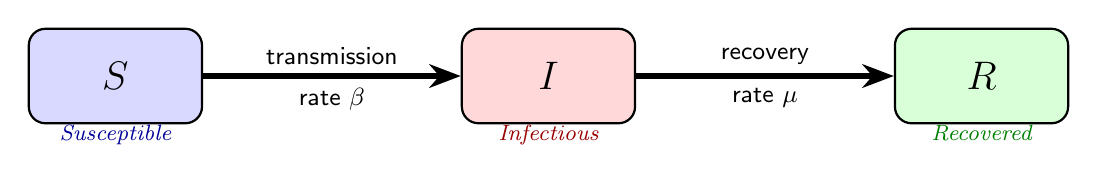
\begin{tikzpicture}[
  comp/.style={draw, rectangle, rounded corners=6pt, minimum width=2.2cm,
               minimum height=1.2cm, font=\bfseries\Large, thick},
  arr/.style={-{Stealth[length=4mm]}, thick, line width=2pt},
  lbl/.style={font=\small\sffamily, above, midway}
]
  \node[comp, fill=blue!15]  (S) at (0,0)    {$S$};
  \node[comp, fill=red!15]   (I) at (5.5,0)  {$I$};
  \node[comp, fill=green!15] (R) at (11.0,0) {$R$};

  \draw[arr] (S) -- node[lbl]{transmission} node[below, font=\small\sffamily, midway]{rate $\beta$} (I);
  \draw[arr] (I) -- node[lbl]{recovery}     node[below, font=\small\sffamily, midway]{rate $\mu$}   (R);

  % state labels below
  \node[font=\footnotesize\itshape, blue!60!black,  below=0.5cm] at (S) {Susceptible};
  \node[font=\footnotesize\itshape, red!60!black,   below=0.5cm] at (I) {Infectious};
  \node[font=\footnotesize\itshape, green!50!black, below=0.5cm] at (R) {Recovered};
\end{tikzpicture}
\end{center}

\subsection{Two Parameters: $\beta$ and $\mu$}

The SIR model is controlled by exactly two numbers:

\begin{conceptbox}{The Two SIR Parameters}
\textbf{$\beta$ (beta) --- Transmission rate.}
The probability per unit time that an infectious person transmits the disease to one susceptible contact. Concretely: if $\beta = 0.3$ per day, then an infectious person infects each of their susceptible contacts with probability $30\%$ per day.

\medskip
\textbf{$\mu$ (mu) --- Recovery rate.}
The probability per unit time that an infectious person recovers. The mean time spent in the infectious state is $1/\mu$ days. If $\mu = 0.1$ per day, the average infectious period is $1/0.1 = 10$ days.

\medskip
\textbf{Units:} Both $\beta$ and $\mu$ have units of $\text{time}^{-1}$ (per day, per hour, etc.), so their ratio $\beta/\mu$ is dimensionless.
\end{conceptbox}

\begin{analogybox}{$\beta$ and $\mu$ as Tap and Drain}
Think of the infectious compartment $I$ as a bucket of water.
\begin{itemize}[noitemsep]
    \item $\beta$ controls the \textbf{tap}: higher $\beta$ means more water flows in (more new infections per day).
    \item $\mu$ controls the \textbf{drain}: higher $\mu$ means water drains faster (people recover sooner).
\end{itemize}
If the tap flows faster than the drain, the bucket fills up (epidemic grows). If the drain wins, the bucket empties (epidemic dies out). The tipping point is exactly $\beta / \mu = 1$, which we will derive shortly.
\end{analogybox}

\subsection{The Differential Equations: Rate of Change of Each Compartment}

We now write down the mathematical rules governing how $S$, $I$, and $R$ change over time. We use \textbf{ordinary differential equations (ODEs)}: $dS/dt$ means ``the rate of change of $S$ with respect to time.'' A positive $dS/dt$ means $S$ is growing; a negative value means $S$ is shrinking.

We derive each equation in words first, then in symbols.

\subsubsection*{Rate of Change of $S$}

Susceptible people leave the $S$ compartment only when they get infected. The rate of new infections per unit time is proportional to:
\begin{itemize}[noitemsep]
    \item The number of infectious people $I(t)$ --- more sick people means more chances of contact.
    \item The number of susceptible people $S(t)$ --- more susceptibles means more people who can be infected.
    \item The transmission rate $\beta$ --- how easily the disease passes per contact.
    \item Divided by $N$ to reflect that contacts are spread across the whole population (well-mixed assumption).
\end{itemize}

This gives the rate $\beta \cdot S(t) \cdot I(t) / N$ new infections per unit time. Since these people \emph{leave} $S$, the sign is negative:

\begin{equation}
\frac{dS}{dt} = -\frac{\beta\, S(t)\, I(t)}{N}
\label{eq:sir_ds}
\end{equation}

\textbf{Reading aloud:} ``The rate of decrease of susceptibles equals beta times S times I, divided by the total population N.''

\subsubsection*{Rate of Change of $I$}

The infectious compartment gains people from $S$ (new infections) and loses people to $R$ (recoveries). The recovery rate is $\mu I(t)$: each of the $I(t)$ currently infectious people recovers at rate $\mu$.

\begin{equation}
\frac{dI}{dt} = \frac{\beta\, S(t)\, I(t)}{N} - \mu\, I(t)
\label{eq:sir_di}
\end{equation}

\textbf{Reading aloud:} ``The rate of change of infectious people equals the inflow of new infections (same magnitude as the outflow from $S$, so opposite sign) minus the outflow of recoveries.''

\subsubsection*{Rate of Change of $R$}

The recovered compartment only gains people from recoveries:

\begin{equation}
\frac{dR}{dt} = \mu\, I(t)
\label{eq:sir_dr}
\end{equation}

\textbf{Consistency check:} Adding all three equations, the $\beta SI/N$ terms cancel:
\[
\frac{dS}{dt} + \frac{dI}{dt} + \frac{dR}{dt} = -\frac{\beta SI}{N} + \frac{\beta SI}{N} - \mu I + \mu I = 0
\]
This means $S + I + R = N$ is constant for all time, as it should be. \checkmark

\begin{mathbox}{The SIR ODE System (Complete)}
\begin{align}
    \frac{dS}{dt} &= -\frac{\beta\, S(t)\, I(t)}{N} \tag{\ref{eq:sir_ds}} \\[4pt]
    \frac{dI}{dt} &= \frac{\beta\, S(t)\, I(t)}{N} - \mu\, I(t) \tag{\ref{eq:sir_di}} \\[4pt]
    \frac{dR}{dt} &= \mu\, I(t) \tag{\ref{eq:sir_dr}}
\end{align}
\textbf{Parameters:} $\beta > 0$ (transmission rate), $\mu > 0$ (recovery rate), $N$ (fixed population).\\
\textbf{Initial conditions:} $S(0) = N - I_0 - R_0$, typically $I_0 = 1$ (one index case), $R_0 = 0$.\\
\textbf{Conservation:} $S(t) + I(t) + R(t) = N$ for all $t \geq 0$.
\end{mathbox}

\subsection{Numerical Simulation by Hand: Euler's Method}

The SIR system has no simple closed-form solution (unlike the SI model). We simulate it numerically using the simplest method: \textbf{Euler's method}. The idea is elementary: if we know the state at time $t$, and we know the \emph{rate of change} at that moment, we can approximate the state at time $t + \Delta t$ by stepping forward:

\[
X(t + \Delta t) \approx X(t) + \frac{dX}{dt}\bigg|_t \cdot \Delta t
\]

``The new value equals the old value plus the rate of change times the time step.''

\begin{examplebox}{Euler's Method Applied to SIR: Step-by-Step Computation}
\textbf{Setup:} $N = 100$, $S(0) = 99$, $I(0) = 1$, $R(0) = 0$, $\beta = 0.3$, $\mu = 0.1$, $\Delta t = 1$ day.

\medskip
\textbf{Step 1: Compute rates at $t = 0$.}
\begin{align*}
    \frac{dS}{dt}\bigg|_0 &= -\frac{0.3 \times 99 \times 1}{100} = -\frac{29.7}{100} = -0.297 \\[4pt]
    \frac{dI}{dt}\bigg|_0 &= +0.297 - 0.1 \times 1 = 0.297 - 0.100 = +0.197 \\[4pt]
    \frac{dR}{dt}\bigg|_0 &= 0.1 \times 1 = +0.100
\end{align*}

\medskip
\textbf{Step 2: Advance to $t = 1$ day.}
\begin{align*}
    S(1) &= S(0) + \frac{dS}{dt}\big|_0 \cdot \Delta t = 99 + (-0.297)(1) = 98.703 \\
    I(1) &= I(0) + \frac{dI}{dt}\big|_0 \cdot \Delta t = 1 + (+0.197)(1) = 1.197 \\
    R(1) &= R(0) + \frac{dR}{dt}\big|_0 \cdot \Delta t = 0 + (+0.100)(1) = 0.100
\end{align*}

\textbf{Check:} $98.703 + 1.197 + 0.100 = 100.000 = N$ \checkmark

\medskip
\textbf{Step 3: Repeat with updated values at $t = 1$.}
\begin{align*}
    \frac{dS}{dt}\bigg|_1 &= -\frac{0.3 \times 98.703 \times 1.197}{100} = -\frac{35.448}{100} = -0.354 \\[4pt]
    \frac{dI}{dt}\bigg|_1 &= +0.354 - 0.1 \times 1.197 = 0.354 - 0.120 = +0.234 \\[4pt]
    \frac{dR}{dt}\bigg|_1 &= 0.1 \times 1.197 = +0.120
\end{align*}
\begin{align*}
    S(2) &= 98.703 - 0.354 = 98.349 \\
    I(2) &= 1.197 + 0.234 = 1.431 \\
    R(2) &= 0.100 + 0.120 = 0.220
\end{align*}

\medskip
\textbf{Three-step summary:}
\begin{center}
\begin{tabular}{ccccc}
\toprule
$t$ & $S(t)$ & $I(t)$ & $R(t)$ & $S+I+R$ \\
\midrule
0 & 99.000 & 1.000 & 0.000 & 100.000 \\
1 & 98.703 & 1.197 & 0.100 & 100.000 \\
2 & 98.349 & 1.431 & 0.220 & 100.000 \\
\bottomrule
\end{tabular}
\end{center}

\textbf{Interpretation:} In the first two days, $I$ is growing (epidemic expanding) while $S$ slowly depletes. The epidemic has not yet peaked.

\medskip
\textbf{Why does $I$ grow?} Because $dI/dt = \beta SI/N - \mu I > 0$ when $\beta S/N > \mu$, i.e., when $S > \mu N/\beta = 0.1 \times 100/0.3 \approx 33$. As long as more than 33 people remain susceptible, the epidemic grows.
\end{examplebox}

\subsection{The Basic Reproduction Number $R_0$}

The single most important quantity in epidemiology is the \textbf{basic reproduction number}, written $R_0$ (pronounced ``R-naught'').

\begin{conceptbox}{The Basic Reproduction Number $R_0$}
$R_0$ is the average number of secondary infections caused by a single infectious individual introduced into a \emph{fully susceptible} population.

In the well-mixed SIR model:
\begin{equation}
    R_0 = \frac{\beta}{\mu}
    \label{eq:r0}
\end{equation}
\textbf{Reading aloud:} ``R-naught equals the transmission rate divided by the recovery rate.''

\textbf{Why this formula?} An infectious person infects at rate $\beta$ per susceptible contact. In a fully susceptible population of size $N$, each person has $\approx N$ potential contacts. The mean infectious duration is $1/\mu$ days. So the total number of secondary infections is $\beta \cdot (1/\mu) = \beta/\mu$.

\textbf{The threshold:}
\begin{itemize}[noitemsep]
    \item If $R_0 > 1$: Each case produces more than one new case on average. The epidemic grows.
    \item If $R_0 = 1$: Exactly self-sustaining. The epidemic neither grows nor shrinks.
    \item If $R_0 < 1$: Each case produces fewer than one new case on average. The epidemic dies out.
\end{itemize}
\end{conceptbox}

\begin{examplebox}{Computing $R_0$ for $\beta = 0.3$, $\mu = 0.1$}
\[
R_0 = \frac{\beta}{\mu} = \frac{0.3}{0.1} = 3
\]
\textbf{Interpretation:} On average, one infected person infects \emph{3 others} (in a fully susceptible population). This is approximately the $R_0$ of seasonal influenza. The epidemic will spread.

For our Euler simulation above ($S(0) = 99 \approx N$, close to fully susceptible): since $R_0 = 3 > 1$, the epidemic grows, as we observed in the computation.

\textbf{To stop the epidemic:} We need to reduce $R_0$ below 1. One way is vaccination: if a fraction $1 - 1/R_0 = 1 - 1/3 \approx 67\%$ of the population is immune, the effective $R_0$ drops below 1. This is the \textbf{herd immunity threshold}.
\end{examplebox}

\begin{center}
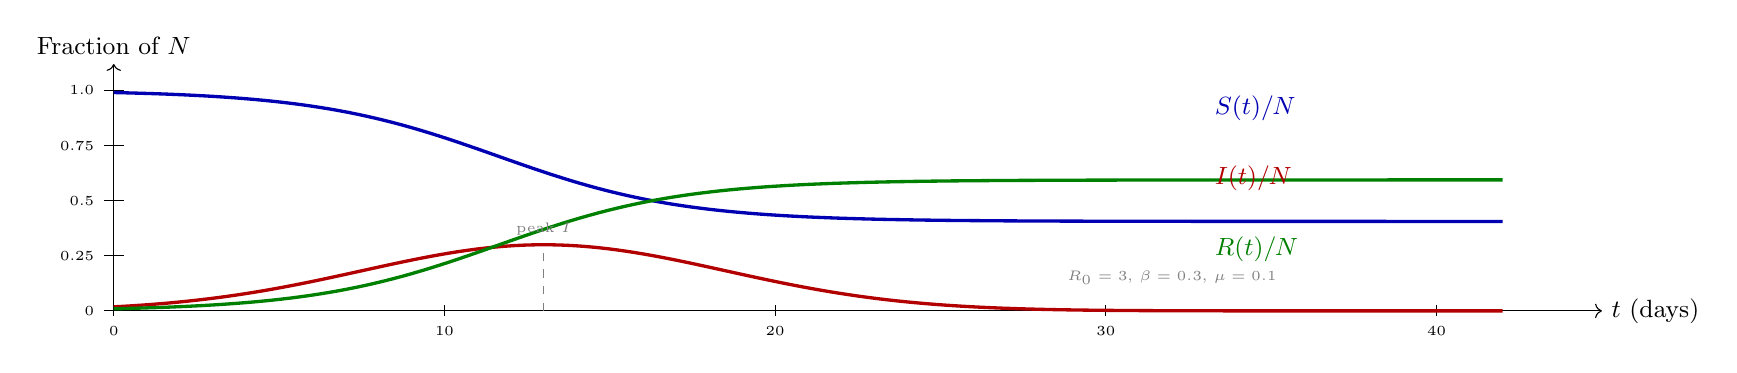
\begin{tikzpicture}[scale=1.0]
\begin{scope}[xscale=0.42, yscale=2.8]
  % Axes
  \draw[->] (0,0) -- (45,0) node[right]{\small $t$ (days)};
  \draw[->] (0,0) -- (0,1.12) node[above]{\small Fraction of $N$};
  \foreach \x in {0,10,20,30,40}{
    \draw (\x,0.025) -- (\x,-0.025) node[below]{\tiny\x};
  }
  \foreach \y in {0,0.25,0.5,0.75,1.0}{
    \draw (0.3,\y) -- (-0.3,\y) node[left]{\tiny\y};
  }
  % Approximate SIR curves: beta=0.3, mu=0.1, R0=3, N=100, S0=99, I0=1
  % S(t): starts near 1, declines to ~0.06 (final size ~94%)
  \draw[blue!70!black, very thick, domain=0:42, samples=150]
    plot (\x, {0.06 + 0.94 * exp(-1.0/(1+exp(-0.35*(\x-13))))});
  % I(t): bell, peaks ~t=13 at ~0.28
  \draw[red!70!black, very thick, domain=0:42, samples=150]
    plot (\x, {0.30*exp(-0.5*((\x-13)/5.5)^2)});
  % R(t): sigmoid from 0 to ~0.94
  \draw[green!50!black, very thick, domain=0:42, samples=150]
    plot (\x, {0.94*(1-exp(-1.0/(1+exp(-0.35*(\x-13)))))});
  % Peak marker
  \draw[gray, dashed] (13, 0) -- (13, 0.30);
  \node[font=\tiny, gray, above] at (13, 0.30) {peak $I$};
  % Legend
  \node[blue!70!black,  font=\small, right] at (33, 0.92) {$S(t)/N$};
  \node[red!70!black,   font=\small, right] at (33, 0.60) {$I(t)/N$};
  \node[green!50!black, font=\small, right] at (33, 0.28) {$R(t)/N$};
  % Annotation: epidemic peak
  \node[font=\tiny, gray] at (32, 0.15) {$R_0 = 3$, $\beta=0.3$, $\mu=0.1$};
\end{scope}
\end{tikzpicture}
\end{center}

\begin{keyinsight}{The Three Phases of an SIR Epidemic}
\begin{enumerate}[noitemsep]
    \item \textbf{Exponential growth} (early stage): $S \approx N$, so $dI/dt \approx \beta I - \mu I = (\beta - \mu) I$. The number of infected grows exponentially at rate $\beta - \mu$. This is why early intervention matters so much.
    \item \textbf{Peak and decline} (middle stage): $S$ has been depleted enough that $\beta S(t)/N < \mu$. New infections no longer outpace recoveries; $I$ peaks and then falls.
    \item \textbf{Burnout} (late stage): the epidemic ends not because everyone is vaccinated, but because there are not enough susceptibles left to sustain transmission. Some susceptibles always survive.
\end{enumerate}
\end{keyinsight}

% ============================================================
\section{The SIR Model on Networks (Network SIR)}
\label{sec:network_sir}
% ============================================================

\subsection{Why the Well-Mixed Assumption Fails}

The well-mixed SIR model assumes that every person can potentially infect every other person. In reality, you can only infect someone you actually meet. Your contacts follow a \textbf{network structure}: your family, colleagues, neighbours, and friends. A hermit with no contacts cannot infect anyone, regardless of how infectious they are. A highly connected person (a doctor, a teacher, a flight attendant) can infect many.

\begin{analogybox}{The Network Changes Everything}
Imagine two towns. Town A is a bus network: everyone goes through the central hub station. Town B is a grid of streets: everyone moves locally. Introduce an infected traveller into the hub of Town A --- the disease reaches all corners of town within days. Introduce the same traveller into a corner of Town B --- the disease spreads slowly, touching each block one by one. Same $\beta$, same $\mu$, same $R_0$. But the dynamics are completely different because the contact \emph{structure} is different.
\end{analogybox}

\subsection{Network SIR: One State per Node}

In the network-aware SIR model, we assign a state $X_i(t) \in \{S, I, R\}$ to \emph{each individual node} $i$. Instead of population-level counts, we track individual fates.

The contact structure is a graph $G = (\mathcal{V}, \mathcal{E})$ where $\mathcal{V}$ is the set of $N$ people (nodes) and $\mathcal{E}$ is the set of contacts (edges). An edge $\{i,j\} \in \mathcal{E}$ means person $i$ and person $j$ are in contact and can transmit the disease to each other.

\subsection{Per-Node Infection Probability}

At each discrete time step, a susceptible node $v$ can be infected by each of its \emph{infectious neighbours} independently. The probability that \emph{at least one} infectious neighbour infects $v$ in one time step is:

\begin{mathbox}{Per-Node Infection Probability (Independent Contacts)}
Let $\mathcal{N}_I(v, t) = \{u \in \mathcal{N}(v) \mid X_u(t) = I\}$ be the set of infectious neighbours of $v$ at time $t$. Each infectious neighbour independently fails to infect $v$ with probability $(1 - \beta)$. All $|\mathcal{N}_I(v,t)|$ must fail for $v$ to remain susceptible. Therefore:

\begin{equation}
    P\bigl(v \text{ gets infected at } t\bigr) = 1 - \prod_{u \in \mathcal{N}_I(v,t)} (1 - \beta)
    = 1 - (1-\beta)^{|\mathcal{N}_I(v,t)|}
    \label{eq:network_infection}
\end{equation}

\textbf{Reading aloud:} ``The probability that $v$ gets infected equals one minus the product over all infectious neighbours of $(1 - \beta)$.''

\textbf{Why a product?} Each infection attempt by a different neighbour is \emph{independent}. The probability that ALL of them fail is the product of each failure probability. One minus that product is the probability that at least one succeeds.
\end{mathbox}

\begin{examplebox}{Computing Infection Probability: Node $v$ with 3 Infected Neighbours}
Node $v$ has 3 infectious neighbours (call them $u_1, u_2, u_3$) and $\beta = 0.2$.

\medskip
\textbf{Step 1:} Each infected neighbour fails to infect $v$ with probability $1 - \beta = 1 - 0.2 = 0.8$.

\medskip
\textbf{Step 2:} All three fail simultaneously with probability $0.8 \times 0.8 \times 0.8 = (0.8)^3 = 0.512$.

\medskip
\textbf{Step 3:} At least one succeeds (i.e., $v$ gets infected) with probability:
\[
P(\text{infected}) = 1 - (0.8)^3 = 1 - 0.512 = \mathbf{0.488}
\]

\textbf{Interpretation:} Even with a relatively low per-contact transmission rate ($\beta = 0.2$), having 3 infected neighbours gives nearly a 50\% chance of being infected in this time step.

\medskip
\textbf{Contrast with 1 infected neighbour:} $P = 1 - 0.8^1 = 0.2$ (exactly $\beta$, as expected).\\
\textbf{With 5 infected neighbours:} $P = 1 - 0.8^5 = 1 - 0.328 = 0.672$ (67\%!).

This shows why \textbf{hubs} (highly connected nodes) are so dangerous: when they are infected, they expose many neighbours simultaneously, driving high infection probabilities even for moderate $\beta$.
\end{examplebox}

\subsection{How the Network Changes Spreading Dynamics}

The network structure modifies both the speed and pattern of spread:

\begin{itemize}
    \item \textbf{Hub nodes} (high degree): a node with degree $k = 50$ can expose 50 people simultaneously. If it becomes infected, it creates a ``burst'' of new cases. In scale-free networks, these hubs collapse the diameter and cause the epidemic to spread much faster than the well-mixed model would predict.
    \item \textbf{Dead-end nodes} (low degree): a node with only 1 contact (a leaf node) can infect at most one person. Stochastic extinction is common from such nodes.
    \item \textbf{Community structure}: if the network consists of tightly-knit clusters connected by a few ``bridge'' edges, the epidemic spreads quickly within each cluster but may take a long time to jump between clusters.
\end{itemize}

\begin{keyinsight}{$R_0$ on a Heterogeneous Network}
In a network where the degree distribution has mean $\langle k \rangle$ and variance $\sigma_k^2$, the effective reproduction number is (via heterogeneous mean-field theory):
\begin{equation}
    R_0^{\mathrm{network}} = \frac{\beta}{\mu} \cdot \frac{\langle k^2 \rangle - \langle k \rangle}{\langle k \rangle}
    \label{eq:r0_network}
\end{equation}
The additional factor $(\langle k^2 \rangle - \langle k \rangle)/\langle k \rangle$ is the \textbf{mean excess degree}: the average number of additional neighbours reachable by following a random edge. For a Poisson degree distribution (Erd\H{o}s-R\'enyi networks), this equals $\langle k \rangle$, recovering $R_0^{\mathrm{network}} = \beta \langle k \rangle / \mu$. For scale-free networks where variance $\sigma_k^2 \gg \langle k \rangle^2$, $R_0^{\mathrm{network}}$ is enormous, explaining why these networks are nearly impossible to make epidemic-free by random vaccination.
\end{keyinsight}

% ============================================================
\section{Temporal SIR on Temporal Networks}
\label{sec:temporal_sir}
% ============================================================

\subsection{Why the Order of Contacts Matters}

In a static network, the edge $\{i, j\}$ says ``$i$ and $j$ are in contact.'' It does not say \emph{when}. This is a problem because diseases cannot travel backwards in time.

\begin{examplebox}{Temporal Order Changes Everything: A 3-Node Example}
Consider three people: Alice (A), Bob (B), and Charlie (C). Suppose the following contacts occur:
\begin{itemize}[noitemsep]
    \item Contact event $e_1$: A meets B at time $t = 1$.
    \item Contact event $e_2$: B meets C at time $t = 2$.
\end{itemize}

\textbf{Scenario 1 (A is the source, infects at $t=1$):}
\begin{itemize}[noitemsep]
    \item At $t=1$: A meets B. A is infected, so B can be infected ($\beta$ transmission attempt). \textbf{Possible path: A $\to$ B $\to$ C.}
    \item At $t=2$: B (if infected) meets C. \textbf{C can be infected by B.}
\end{itemize}

\textbf{Now reverse the order of events:} Suppose instead:
\begin{itemize}[noitemsep]
    \item Contact event $e_1'$: B meets C at time $t = 1$.
    \item Contact event $e_2'$: A meets B at time $t = 2$.
\end{itemize}

\textbf{Scenario 2 (same contacts, different order, A is the source):}
\begin{itemize}[noitemsep]
    \item At $t=1$: B meets C. A is still the only infected person. B is susceptible, so \textbf{nothing happens} (no transmission source for C from B yet).
    \item At $t=2$: A meets B. Now B can be infected. But the B--C contact already happened at $t=1$ when B was susceptible. \textbf{C cannot be infected via B.}
\end{itemize}

\textbf{Result:} Same contact graph (A--B--C path), same parameters, same source (A). But Scenario 1 allows C to be infected, while Scenario 2 does not. The temporal order of contacts is the difference.
\end{examplebox}

\begin{center}
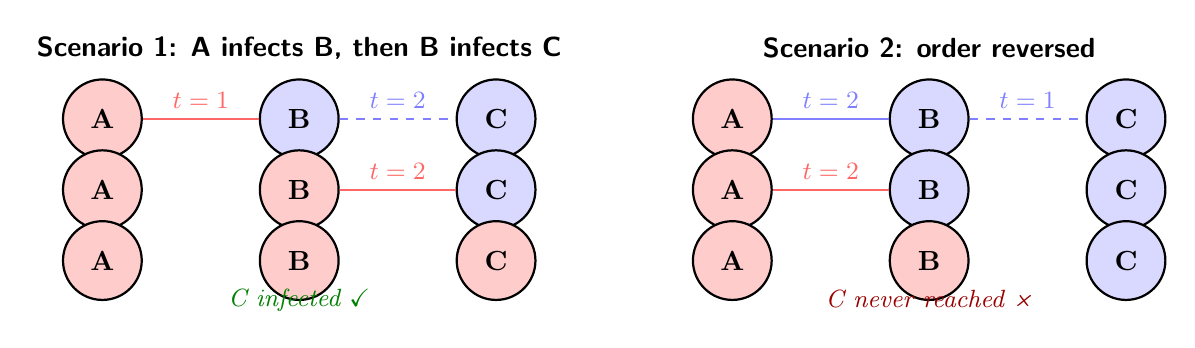
\begin{tikzpicture}[
  pnode/.style={draw, circle, minimum size=1.0cm, font=\bfseries, thick},
  Sn/.style={pnode, fill=blue!15},
  In/.style={pnode, fill=red!20},
  arr/.style={-{Stealth[length=3mm]}, thick}
]
% Scenario 1
\node[font=\bfseries\sffamily] at (2.5, 3.3) {Scenario 1: A infects B, then B infects C};

\node[In]  (A1) at (0.0, 2.4) {A};
\node[Sn]  (B1) at (2.5, 2.4) {B};
\node[Sn]  (C1) at (5.0, 2.4) {C};
\draw[thick, red!60] (A1) -- node[above, font=\small]{$t=1$} (B1);
\draw[thick, blue!50, dashed] (B1) -- node[above, font=\small]{$t=2$} (C1);

\node[In]  (A1b) at (0.0, 1.5) {A};
\node[In]  (B1b) at (2.5, 1.5) {B};
\node[Sn]  (C1b) at (5.0, 1.5) {C};
\draw[thick, red!60] (B1b) -- node[above, font=\small]{$t=2$} (C1b);

\node[In]  (A1c) at (0.0, 0.6) {A};
\node[In]  (B1c) at (2.5, 0.6) {B};
\node[In]  (C1c) at (5.0, 0.6) {C};
\node[font=\small\itshape, green!50!black] at (2.5, 0.1) {C infected \checkmark};

% Scenario 2
\node[font=\bfseries\sffamily] at (10.5, 3.3) {Scenario 2: order reversed};

\node[In]  (A2) at (8.0, 2.4) {A};
\node[Sn]  (B2) at (10.5, 2.4) {B};
\node[Sn]  (C2) at (13.0, 2.4) {C};
\draw[thick, blue!50, dashed] (B2) -- node[above, font=\small]{$t=1$} (C2);
\draw[thick, blue!50] (A2) -- node[above, font=\small]{$t=2$} (B2);

\node[In]  (A2b) at (8.0, 1.5) {A};
\node[Sn]  (B2b) at (10.5, 1.5) {B};
\node[Sn]  (C2b) at (13.0, 1.5) {C};
\draw[thick, red!60] (A2b) -- node[above, font=\small]{$t=2$} (B2b);

\node[In]  (A2c) at (8.0, 0.6) {A};
\node[In]  (B2c) at (10.5, 0.6) {B};
\node[Sn]  (C2c) at (13.0, 0.6) {C};
\node[font=\small\itshape, red!60!black] at (10.5, 0.1) {C never reached \texttimes};

\end{tikzpicture}

\vspace{0.5em}
\small\itshape
Red solid edges: active transmission. Blue dashed edges: contact with no transmission (one side not yet infected). Same network topology, same parameters --- different temporal order gives a different outcome.
\end{center}

\subsection{Temporal Networks as Event Sequences}

A \textbf{temporal network} $G^T = (\mathcal{V}, E^T)$ is a list of timestamped contact events:
\[
E^T = \{(u_1, v_1, t_1),\; (u_2, v_2, t_2),\; \ldots,\; (u_m, v_m, t_m)\}
\]
where each triple $(u, v, t)$ means ``person $u$ and person $v$ were in contact at time $t$.'' The events are sorted by time: $t_1 \leq t_2 \leq \cdots \leq t_m$.

\subsection{Discrete-Time Temporal SIR: The Simulation Rule}

The simulation processes events in chronological order. At each contact event $(u, v, t)$:

\begin{conceptbox}{The Temporal SIR Update Rule}
When a contact event $(u, v, t)$ is processed:
\begin{enumerate}[noitemsep]
    \item \textbf{Attempt infection} from $u$ to $v$: if $X_u(t) = I$ and $X_v(t) = S$, then $v$ becomes infected with probability $\beta$. (Draw a uniform random number; if it is $< \beta$, set $X_v \leftarrow I$.)
    \item \textbf{Attempt infection} from $v$ to $u$: symmetrically, if $X_v(t) = I$ and $X_u(t) = S$, then $u$ becomes infected with probability $\beta$.
    \item \textbf{Recovery}: between events, each infectious node $i$ recovers with probability $\mu$ per unit time. In an event-driven simulation, this is handled by sampling the recovery time for each node when they become infected.
\end{enumerate}
\end{conceptbox}

\begin{conceptbox}{The Infectious Window}
A node can only spread the infection while it is in state $I$. Once a node recovers (transitions to $R$), any subsequent contact events involving that node are irrelevant for transmission. This is the \textbf{infectious window}: the time interval between a node's infection time and recovery time.

If node $i$ is infected at time $t_{\text{inf}}$ and recovers at time $t_{\text{rec}} \sim \text{Exponential}(\mu)$, then node $i$ can only infect neighbours during the interval $[t_{\text{inf}}, t_{\text{rec}})$. Contact events $(i, j, t)$ with $t \geq t_{\text{rec}}$ are ignored.

This creates an \textbf{asymmetry}: if $i$ infects $j$ early in its infectious window, $j$ has the rest of the observation period to potentially spread further. If $i$ infects $j$ late, $j$ has little time. The temporal structure of the contact sequence directly shapes the final outbreak pattern.
\end{conceptbox}

\begin{examplebox}{Three Nodes, Two Events: Computing Temporal SIR by Hand}
\textbf{Network:} 3 nodes $\{A, B, C\}$. Events: $(A, B, t=2)$ and $(B, C, t=5)$.

\textbf{Parameters:} $\beta = 0.6$. Recovery times are drawn from Exponential($\mu=0.1$), so mean infectious period $= 10$ time units.

\textbf{Initial state:} $A$ is infected at $t=0$ (source). $B$ and $C$ are susceptible.

\textbf{Draw recovery time for A:} Suppose $t_{\text{rec}}(A) = 8$ (a random sample).

\medskip
\textbf{Process event $(A, B, t=2)$:}
\begin{itemize}[noitemsep]
    \item $t = 2 < t_{\text{rec}}(A) = 8$ --- A is still infectious. \checkmark
    \item $X_B(2) = S$ --- B is susceptible. \checkmark
    \item Draw $U \sim \text{Uniform}(0,1)$. Suppose $U = 0.41 < \beta = 0.6$. \textbf{B gets infected.}
    \item Draw $t_{\text{rec}}(B) \sim \text{Exponential}(0.1)$. Suppose $t_{\text{rec}}(B) = 13$.
\end{itemize}

\textbf{Process event $(B, C, t=5)$:}
\begin{itemize}[noitemsep]
    \item $t = 5 < t_{\text{rec}}(B) = 13$ --- B is still infectious. \checkmark
    \item $X_C(5) = S$ --- C is susceptible. \checkmark
    \item Draw $U = 0.75 > \beta = 0.6$. \textbf{C is not infected.} (Lucky escape.)
\end{itemize}

\textbf{Final state (after all recoveries):} $A \in R$, $B \in R$, $C \in S$. Only $A$ and $B$ were infected.

\textbf{If instead $t_{\text{rec}}(A) = 1$ (recovers before $t=2$):} Then event $(A, B, t=2)$ does nothing (A already in $R$), and the entire epidemic dies with only A infected. The randomness of recovery timing creates dramatically different outcomes from the same source.
\end{examplebox}

% ============================================================
\section{Stochastic Simulations (Monte Carlo)}
\label{sec:monte_carlo}
% ============================================================

\subsection{Why One Run Is Not Enough}

The temporal SIR process is \textbf{stochastic} (random). Given a fixed source node $v_0$ and fixed parameters $\beta$ and $\mu$, running the simulation twice will generally produce two different final states. Sometimes the epidemic explodes and infects 80\% of the network; sometimes it dies out after 3 nodes. Both outcomes can arise from the same source.

\begin{analogybox}{Stochastic Epidemics as Dice Rolls}
Imagine rolling a die at each contact event: if you roll a 1 or 2 (on a six-sided die, i.e., $\beta = 1/3$), the infection passes. Each ``run'' is a different sequence of dice rolls. Run the experiment 1000 times and you see the full distribution of outcomes: sometimes all dice roll high (big outbreak), sometimes all roll low (early extinction). The probability distribution over outcomes characterises the source's epidemiological ``fingerprint.''
\end{analogybox}

This randomness means that to characterise how a source behaves, we must run \textbf{many} simulations and look at the distribution. This is \textbf{Monte Carlo simulation}: using random sampling to estimate probability distributions.

\subsection{Terminology: $n\_\text{runs}$ and $\text{mc\_runs}$}

The project codebase distinguishes two roles for simulations:

\begin{conceptbox}{Two Types of Simulation Runs}
\textbf{\texttt{n\_runs}} (ground-truth runs): For each candidate source node $v_0 \in \mathcal{V}$, we run \texttt{n\_runs} independent SIR simulations from $v_0$. These high-statistics runs are used to compute the \emph{ground-truth likelihood} $P(\mathcal{O} \mid \text{source} = v_0)$. Default: \texttt{n\_runs} = 5000.

\medskip
\textbf{\texttt{mc\_runs}} (Monte Carlo training runs): Additional simulations run from each node, used to generate \emph{training data} for the GNN. These are observations the model learns from. Default: \texttt{mc\_runs} = 500.

\medskip
\textbf{Why different sizes?} The ground-truth likelihood needs high precision (5000 runs $\to$ standard error $\leq 0.007$) because it is the reference we compare against. Training data can tolerate more noise (500 runs) to keep data generation tractable.
\end{conceptbox}

\subsection{Pseudocode for a Single Temporal SIR Simulation}

\begin{codewalk}{Single Temporal SIR Simulation: Pseudocode}
\begin{lstlisting}[language=Python]
def run_temporal_sir(events, n_nodes, beta, mu, source):
    """
    Run one stochastic SIR simulation on a temporal network.

    Parameters
    ----------
    events   : list of (u, v, t) triples, sorted by ascending t
    n_nodes  : total number of nodes
    beta     : transmission probability per contact event
    mu       : recovery rate (per unit time)
    source   : index of the initial infectious node

    Returns
    -------
    state    : np.array of shape (n_nodes,), dtype int8
               0 = Susceptible, 1 = Infected, 2 = Recovered
               (state at the END of the simulation)
    """
    # --- Initialisation ---
    state = np.zeros(n_nodes, dtype=int8)      # all Susceptible
    state[source] = 1                           # source is Infected
    infection_time = {source: 0.0}             # when each node was infected
    recovery_time  = {}                         # when each node will recover

    # Draw recovery time for the source
    recovery_time[source] = 0.0 + sample_exponential(mu)

    # --- Process events in chronological order ---
    for (u, v, t) in sorted(events, key=lambda e: e[2]):

        # Attempt infection u -> v
        if state[u] == 1 and state[v] == 0:         # u infectious, v susceptible
            if t < recovery_time[u]:                 # u still in infectious window
                if random.uniform(0,1) < beta:       # transmission succeeds
                    state[v] = 1
                    infection_time[v] = t
                    recovery_time[v] = t + sample_exponential(mu)

        # Attempt infection v -> u (symmetric)
        if state[v] == 1 and state[u] == 0:
            if t < recovery_time[v]:
                if random.uniform(0,1) < beta:
                    state[u] = 1
                    infection_time[u] = t
                    recovery_time[u] = t + sample_exponential(mu)

    # --- Mark all infectious nodes as Recovered at end ---
    for i in range(n_nodes):
        if state[i] == 1:
            state[i] = 2

    return state
\end{lstlisting}
\textbf{Key points:}
\begin{itemize}[noitemsep]
    \item Events are processed in time order (line 23). This enforces the causal ordering.
    \item The \texttt{recovery\_time[u]} check (line 26) implements the infectious window.
    \item \texttt{sample\_exponential(mu)} returns a sample from the exponential distribution with mean $1/\mu$.
    \item The output is a flat array of shape \texttt{(n\_nodes,)} with values in $\{0, 1, 2\}$ for $\{S, I, R\}$.
\end{itemize}
\end{codewalk}

\subsection{The Output: Binary Arrays and Their Shape}

Running \texttt{n\_runs} simulations from a single source node $v_0$ produces \texttt{n\_runs} state vectors, each of shape \texttt{(n\_nodes,)}. Stacking them gives an array of shape \texttt{(n\_runs, n\_nodes)}.

When we run \texttt{n\_runs} simulations from \emph{every} possible source node, we get an array of shape \texttt{(n\_nodes, n\_runs, n\_nodes)}.

\begin{conceptbox}{The \texttt{truth\_S/I/R} Array Shape: \texttt{(n\_nodes, n\_runs, n\_nodes)}}
The three arrays \texttt{truth\_S}, \texttt{truth\_I}, \texttt{truth\_R} each have shape \texttt{(n\_nodes, n\_runs, n\_nodes)} and contain values in $\{0, 1\}$ (int8).

\textbf{Axis 0 --- source node index:} Which node was used as the source for this batch of simulations. \texttt{truth\_I[v, :, :]} contains all simulation runs with source $v$.

\textbf{Axis 1 --- simulation run index:} The run number within the batch. \texttt{truth\_I[v, r, :]} is the state vector from the $r$-th run with source $v$.

\textbf{Axis 2 --- node state:} Whether each node is in state $I$ (or $S$, or $R$) at the end. \texttt{truth\_I[v, r, j] = 1} means node $j$ was infectious at the end of run $r$ with source $v$.

\textbf{Example access:}
\begin{lstlisting}[language=Python]
# Fraction of runs from source v=3 in which node j=7 was infected:
fraction_infected = truth_I[3, :, 7].mean()   # mean over all n_runs

# All final states from source v=0, run r=42:
state_vector = truth_I[0, 42, :]   # shape (n_nodes,)
\end{lstlisting}

\medskip
\textbf{Memory:} For $N = 500$ nodes, $n\_\text{runs} = 5000$: each array is $500 \times 5000 \times 500 = 1.25 \times 10^9$ entries. At 1 byte (int8) each, that is approximately 1.25 GB per array (times 3 for S, I, R). This is why the simulation data is stored in compact binary \texttt{.bin} files and loaded via \texttt{np.fromfile}.
\end{conceptbox}

Similarly, the Monte Carlo training arrays \texttt{mc\_S/I/R} have shape \texttt{(n\_nodes, mc\_runs, n\_nodes)}, where \texttt{mc\_runs} $\ll$ \texttt{n\_runs}.

% ============================================================
\section{The TSIR C Implementation}
\label{sec:tsir_code}
% ============================================================

\subsection{Why C for Simulation?}

Running $N \times n\_\text{runs}$ simulations in Python would take hours. The project uses an event-driven C implementation of temporal SIR adapted from Petter Holme's \texttt{tsir} codebase (see \cite{holme2020fast}), wrapped in a Python interface. The C code processes all events for all nodes in a tight loop with no Python interpreter overhead, achieving speedups of 100--1000$\times$ over equivalent Python code.

\subsection{The Python Wrapper: How to Call the Simulation}

\begin{codewalk}{Calling the TSIR C Engine from Python (\texttt{tsir/read\_run.py})}
The Python layer provides three functions, each running the C binary with different parameters:

\begin{lstlisting}[language=Python]
from tsir.read_run import tsir, make_c_readable_from_nparray

# Step 1: Convert the temporal network to the C-readable text format.
# H_array is a NumPy array of shape (n_events, 3) with columns [u, v, t].
H_cedges = make_c_readable_from_nparray(H_array, end_t, n_nodes)

# Step 2: Configure the simulation.
tsir_config = {
    "sir": {
        "beta":    0.3,    # transmission rate
        "mu":      0.1,    # recovery rate
        "start_t": 0,      # first event time to include
        "end_t":   50,     # last event time (observation cutoff)
        "n_runs":  5000    # number of simulations per source
    },
    "nwk": {
        "directed": False  # undirected contact network
    }
}

# Step 3: Run the simulation.
# Returns three arrays: log-probabilities of S, I, R per node.
tsir_S, tsir_I, tsir_R = tsir(tsir_config, H_cedges, n_nodes)
\end{lstlisting}

Internally, \texttt{tsir()} calls the compiled C binary \texttt{./tsir/tsir} via subprocess, passing the network as a pipe, and reads back three binary \texttt{.bin} files containing the output arrays.
\end{codewalk}

\subsection{The Ground-Truth and Monte Carlo Functions}

The \texttt{read\_run.py} module exposes two higher-level functions that wrap the C binary for the two use cases:

\begin{codewalk}{Ground-Truth and Monte Carlo Runs (\texttt{tsir/read\_run.py})}
\begin{lstlisting}[language=Python]
# --- Ground-truth run (high n_runs, one per source node) ---
truth_S, truth_I, truth_R = sir_ground_truth(cfg, H_cread, n_nodes, local_folder)
# Output shapes: (n_nodes, n_runs, n_nodes) each, dtype=int8

# --- Monte Carlo run (lower mc_runs, for training data) ---
mc_S, mc_I, mc_R = sir_monte_carlo(cfg, H_cread, n_nodes, local_folder)
# Output shapes: (n_nodes, mc_runs, n_nodes) each, dtype=int8
\end{lstlisting}

Both functions:
\begin{itemize}[noitemsep]
    \item Call the C binary with \texttt{cfg.sir.beta}, \texttt{cfg.sir.mu}, etc. from the YAML config.
    \item Write output to binary \texttt{.bin} files (e.g., \texttt{ground\_truth\_I.bin}).
    \item Load the binary files with \texttt{np.fromfile(..., dtype=np.int8)} and reshape to the correct 3D shape.
    \item Log the estimated $R_0$, average outbreak size, and standard error to \texttt{wandb}.
\end{itemize}

\textbf{Binary file format:} Each \texttt{.bin} file is a flat array of \texttt{int8} values. For the ground-truth I-state file: the file has $n\_\text{nodes} \times n\_\text{runs} \times n\_\text{nodes}$ bytes, where byte at position $v \cdot n\_\text{runs} \cdot n\_\text{nodes} + r \cdot n\_\text{nodes} + j$ is $1$ if node $j$ was in state $I$ at the end of run $r$ from source $v$, and $0$ otherwise.
\end{codewalk}

\subsection{The \texttt{TSIRData} Dataclass: Centralized Data Access}

Once the simulation files are loaded, all arrays are packaged into a single \texttt{TSIRData} dataclass (defined in \texttt{setup/data\_loader.py}) that is passed to every downstream method:

\begin{codewalk}{The \texttt{TSIRData} Dataclass (\texttt{setup/data\_loader.py})}
\begin{lstlisting}[language=Python]
@dataclass
class TSIRData:
    config:           dict           # YAML config used for this simulation
    n_nodes:          int            # N: number of nodes in the network
    n_runs:           int            # number of ground-truth runs per source
    mc_runs:          int            # number of MC training runs per source

    mc_S:             np.ndarray     # shape (n_nodes, mc_runs,  n_nodes), int8
    mc_I:             np.ndarray     # shape (n_nodes, mc_runs,  n_nodes), int8
    mc_R:             np.ndarray     # shape (n_nodes, mc_runs,  n_nodes), int8

    truth_S:          np.ndarray     # shape (n_nodes, n_runs,   n_nodes), int8
    truth_I:          np.ndarray     # shape (n_nodes, n_runs,   n_nodes), int8
    truth_R:          np.ndarray     # shape (n_nodes, n_runs,   n_nodes), int8

    maximal_outbreak: np.ndarray     # shape (n_nodes, n_nodes),  int8
    possible:         np.ndarray     # shape (n_nodes, n_runs, n_nodes), int8
    lik_possible:     np.ndarray     # shape (n_nodes, n_runs, n_nodes), float
\end{lstlisting}

\textbf{The two mask arrays:}
\begin{itemize}[noitemsep]
    \item \textbf{\texttt{maximal\_outbreak}}: shape \texttt{(n\_nodes, n\_nodes)}. Entry \texttt{[v, j] = 1} if node $j$ is reachable from source $v$ when $\beta=1$, $\mu=0$ (perfect spreading). Defines the \emph{maximum possible outbreak} from each source.
    \item \textbf{\texttt{possible}}: shape \texttt{(n\_nodes, n\_runs, n\_nodes)}. Entry \texttt{[v, r, j] = 1} if the observation in run $r$ is \emph{consistent} with source $v$ (i.e., no node is infected that could not have been reached from $v$). Used to filter out physically impossible source hypotheses.
\end{itemize}
\end{codewalk}

% ============================================================
\section{The Source Detection Problem: Formal Statement}
\label{sec:source_detection_problem}
% ============================================================

\subsection{The Setup}

We now have all the tools to define the source detection problem precisely. An epidemic has run on a temporal network. At observation time $T$, we record who is in each compartment:

\begin{conceptbox}{The Observed Outbreak $\mathcal{O}$}
The \textbf{observation} $\mathcal{O}$ at time $T$ is a mapping from nodes to states:
\[
\mathcal{O} = \{X_i(T) : i \in \mathcal{V}\}, \quad X_i(T) \in \{S, I, R\}
\]
Equivalently, $\mathcal{O}$ specifies three sets:
\begin{itemize}[noitemsep]
    \item $\mathcal{V}_S = \{i : X_i(T) = S\}$ --- nodes that were never infected by time $T$.
    \item $\mathcal{V}_I = \{i : X_i(T) = I\}$ --- nodes currently infectious at time $T$.
    \item $\mathcal{V}_R = \{i : X_i(T) = R\}$ --- nodes that were infected and have recovered.
\end{itemize}
The ``infected set'' is $\mathcal{V}_{IR} = \mathcal{V}_I \cup \mathcal{V}_R$: all nodes ever infected.
\end{conceptbox}

\subsection{The Source Detection Problem}

\begin{conceptbox}{Formal Problem Statement}
\textbf{Given:}
\begin{itemize}[noitemsep]
    \item A temporal contact network $G^T = (\mathcal{V}, E^T)$.
    \item An observed outbreak state $\mathcal{O}$ (who is $S$, $I$, $R$ at observation time $T$).
    \item Model parameters $\beta$ and $\mu$.
\end{itemize}

\textbf{Find:} The most likely source node:
\begin{equation}
    v^* = \underset{v \in \mathcal{V}}{\mathrm{argmax}} \; P\bigl(\mathcal{O} \mid \text{source} = v,\; \beta,\; \mu\bigr)
    \label{eq:source_detection}
\end{equation}

\textbf{Reading aloud:} ``$v^*$ is the node $v$ in $\mathcal{V}$ that maximises the probability of observing the outbreak $\mathcal{O}$, given that $v$ is the source and the parameters are $\beta$ and $\mu$.''

This is a \textbf{maximum likelihood estimator (MLE)} for the source: we choose the source hypothesis that makes the observed data most probable under the model.
\end{conceptbox}

\subsection{Computing the Likelihood: The Simulation-Based Approach}

How do we compute $P(\mathcal{O} \mid \text{source} = v)$? In general, there is no closed-form formula. Instead, we estimate it by simulation:

\begin{mathbox}{Monte Carlo Likelihood Estimation}
Run $M = \texttt{n\_runs}$ independent simulations from source $v$ under the SIR model. Let $\mathcal{O}^{(1)}, \mathcal{O}^{(2)}, \ldots, \mathcal{O}^{(M)}$ be the resulting observations. Then:
\begin{equation}
    P(\mathcal{O} \mid \text{source} = v) \approx \frac{1}{M} \sum_{m=1}^{M} \mathbf{1}\bigl[\mathcal{O}^{(m)} = \mathcal{O}\bigr]
    \label{eq:mc_likelihood}
\end{equation}

\textbf{Reading aloud:} ``The probability of observation $\mathcal{O}$ given source $v$ is estimated by the fraction of simulation runs from $v$ that produce exactly the observation $\mathcal{O}$.''

\textbf{Statistical precision:} With $M = 5000$ runs, the standard error on this estimate is at most $1/(2\sqrt{5000}) \approx 0.007$, giving an accuracy of $\pm 0.7\%$.
\end{mathbox}

\begin{analogybox}{The Likelihood as a Fingerprint Match}
Each source node produces a characteristic distribution over outbreak shapes --- its ``fingerprint.'' To identify the source, we compare the observed outbreak against every source's fingerprint and ask: ``which fingerprint matches best?'' A source located at the geographic centre of the infected set will produce outbreaks that look like the observation much more often than a source at the periphery. The MLE source is the node whose fingerprint most closely matches what we see.
\end{analogybox}

\subsection{Why MLE Alone Is Too Slow}

The maximum likelihood approach requires running $O(N \times \texttt{n\_runs})$ simulations: for each of the $N$ candidate source nodes, we run \texttt{n\_runs} simulations. With $N = 500$ nodes and \texttt{n\_runs} = 5000:
\[
500 \times 5000 = 2{,}500{,}000 \text{ simulations}
\]

Even with the fast C implementation, this is the bottleneck. Moreover, at \emph{inference time} (when we have a new observation to analyse), we would need to re-run all simulations. This does not scale.

\begin{keyinsight}{Why We Need GNNs}
The GNN's role is to \emph{learn} the likelihood function from pre-computed training data. Given an observation $\mathcal{O}$ as input, the GNN outputs a probability distribution over source nodes --- essentially approximating $P(\text{source} = v \mid \mathcal{O})$ for all $v$ simultaneously, in a single forward pass. Training is expensive (done once), but inference is fast (milliseconds). This is the fundamental motivation for the neural approach.
\end{keyinsight}

% ============================================================
\section{The Basic Reproduction Number $R_0$: Deeper Analysis}
\label{sec:r0_deep}
% ============================================================

\subsection{Deriving $R_0$ from the SIR Equations}

We can derive $R_0$ rigorously from the SIR equations by examining the early epidemic dynamics. At the very start of the epidemic, $S(0) \approx N$ (nearly fully susceptible). Equation~\eqref{eq:sir_di} becomes:
\[
\frac{dI}{dt} \approx \beta I - \mu I = (\beta - \mu) I
\]
This is exponential growth at rate $(\beta - \mu)$: positive when $\beta > \mu$, i.e., when $\beta/\mu > 1$.

The epidemic grows iff $R_0 = \beta/\mu > 1$. It declines iff $R_0 < 1$.

\begin{examplebox}{$R_0$ Computation and Interpretation for Common Parameter Sets}
\begin{center}
\begin{tabular}{cccll}
\toprule
$\beta$ & $\mu$ & $R_0 = \beta/\mu$ & Mean infectious period & Interpretation \\
\midrule
0.3 & 0.1 & 3.0 & 10 days & Influenza-like. Epidemic grows. \\
0.2 & 0.4 & 0.5 & 2.5 days & Epidemic dies out immediately. \\
0.1 & 0.1 & 1.0 & 10 days & Critical point; borderline. \\
0.5 & 0.1 & 5.0 & 10 days & Highly contagious (e.g., measles $\approx 12$--18). \\
\bottomrule
\end{tabular}
\end{center}

\textbf{For $\beta = 0.3$, $\mu = 0.1$, $R_0 = 3$:} In a fully susceptible population, one infected person infects 3 others, each of whom infects 3 more: $1 \to 3 \to 9 \to 27 \to \ldots$ This exponential growth continues until susceptibles are depleted.

\textbf{The herd immunity threshold:} To stop the epidemic, enough people must be immune. If a fraction $f$ of the population is immune, the effective $R_0$ becomes $R_0 \cdot (1-f)$. We need $R_0 \cdot (1-f) < 1$, i.e.:
\[
f > 1 - \frac{1}{R_0} = 1 - \frac{1}{3} \approx 67\%
\]
We must vaccinate at least 67\% of the population to prevent an epidemic when $R_0 = 3$.
\end{examplebox}

\subsection{$R_0$ on Heterogeneous Networks: The Effect of Hubs}

In a well-mixed population, $R_0 = \beta/\mu$. On a network, highly connected nodes (hubs) dramatically increase the effective $R_0$. Recall Equation~\eqref{eq:r0_network}:
\[
R_0^{\mathrm{network}} = \frac{\beta}{\mu} \cdot \frac{\langle k^2 \rangle - \langle k \rangle}{\langle k \rangle}
\]

\begin{examplebox}{$R_0$ Comparison: Erd\H{o}s-R\'enyi vs.\ Barab\'asi-Albert, $\langle k \rangle = 6$, $\beta = 0.3$, $\mu = 0.1$}
\textbf{Erd\H{o}s-R\'enyi (Poisson degree distribution):} $\sigma_k^2 = \langle k \rangle = 6$, so $\langle k^2 \rangle = \langle k \rangle^2 + \sigma_k^2 = 36 + 6 = 42$.
\[
R_0^{\mathrm{ER}} = \frac{0.3}{0.1} \cdot \frac{42 - 6}{6} = 3 \cdot 6 = 18
\]

\textbf{Barab\'asi-Albert (power-law degree distribution):} For $N = 1000$ and $\langle k \rangle = 6$, numerical estimates give $\langle k^2 \rangle \approx 120$ (much larger due to hubs).
\[
R_0^{\mathrm{BA}} = \frac{0.3}{0.1} \cdot \frac{120 - 6}{6} = 3 \cdot 19 = 57
\]

\textbf{The same disease is more than 3$\times$ more dangerous in a hub-structured network.} The hubs act as super-spreaders: when infected, they can infect dozens of neighbours simultaneously.

\textbf{Implication for source detection:} In scale-free networks, high-degree nodes are both more likely to become infected (more contacts) and more likely to be the source (they can generate large outbreaks). This is why the \textbf{degree baseline} (predicting the highest-degree node as the source) performs non-trivially as a heuristic.
\end{examplebox}

\begin{keyinsight}{The Spectral Epidemic Threshold: A Sharper Condition}
The mean-field $R_0$ is an approximation. A rigorous condition for epidemic spread on a specific network uses the \textbf{spectral radius} $\lambda_1$ of the adjacency matrix $\mathbf{A}$ (its largest eigenvalue). The epidemic can spread if and only if:
\begin{equation}
    \frac{\beta}{\mu} > \frac{1}{\lambda_1(\mathbf{A})}
    \label{eq:spectral_threshold}
\end{equation}
For a regular graph of degree $k$, $\lambda_1 = k$ and this reduces to $\beta k / \mu > 1$, consistent with intuition. This connection between spectral graph theory (Chapter~1) and epidemic thresholds is fundamental: the structure of the network --- encoded in $\mathbf{A}$ --- directly determines whether an epidemic can grow.
\end{keyinsight}

% ============================================================
\section{Chapter Summary}
\label{sec:epi_summary}
% ============================================================

This chapter has built the complete epidemiological toolkit used throughout this thesis:

\begin{conceptbox}{What We Have Established}
\begin{enumerate}[noitemsep]
    \item \textbf{The SIR model} partitions individuals into Susceptible ($S$), Infectious ($I$), and Recovered ($R$) states. Two parameters control everything: $\beta$ (transmission rate) and $\mu$ (recovery rate). The conservation law $S + I + R = N$ holds at all times.

    \item \textbf{The SIR ODEs:} $dS/dt = -\beta SI/N$; $dI/dt = \beta SI/N - \mu I$; $dR/dt = \mu I$. Euler's method advances the state step by step: starting from $S(0)=99$, $I(0)=1$, $R(0)=0$ with $\beta=0.3$, $\mu=0.1$, we computed $I(1) \approx 1.197$ and $I(2) \approx 1.431$.

    \item \textbf{Network SIR} assigns one state per node. Infection probability at node $v$ with $k$ infectious neighbours: $P = 1 - (1-\beta)^k$. For $k=3$, $\beta=0.2$: $P = 1 - 0.8^3 = 0.488$.

    \item \textbf{Temporal SIR} processes contact events $(u, v, t)$ in chronological order. The infectious window concept ensures causality: only contacts \emph{during} a node's infection are relevant. Reversing the temporal order of contacts changes which nodes are reachable.

    \item \textbf{Monte Carlo simulation} runs $\texttt{n\_runs}$ independent realisations from each candidate source. Output arrays have shape \texttt{(n\_nodes, n\_runs, n\_nodes)} with axes: [source node, simulation run, node state]. Stored as compact \texttt{int8} binary files.

    \item \textbf{The TSIR C engine} (\texttt{tsir/}) implements event-driven temporal SIR in optimised C, wrapped by Python functions \texttt{sir\_ground\_truth} and \texttt{sir\_monte\_carlo}. Results are packaged into the \texttt{TSIRData} dataclass.

    \item \textbf{The source detection problem:} $v^* = \mathrm{argmax}_v\, P(\mathcal{O} \mid \text{source}=v)$. The MLE is accurate but computationally expensive ($O(N \times \texttt{n\_runs})$ simulations). The GNN learns to approximate this likelihood function in a single forward pass.

    \item \textbf{$R_0 = \beta/\mu$:} Epidemic grows iff $R_0 > 1$. For $\beta=0.3$, $\mu=0.1$: $R_0=3$, meaning each infected person infects 3 others on average. On heterogeneous networks, hub nodes inflate the effective $R_0$ via the excess-degree factor $(\langle k^2 \rangle - \langle k \rangle)/\langle k \rangle$.
\end{enumerate}

\textbf{Coming up:} Chapter~4 formalises the source detection task as a machine learning problem and introduces the classical algorithms (rumour centrality, Jordan centre, soft margin estimator) that serve as baselines for our GNN models.
\end{conceptbox}


% Part II: Source Detection Theory
\part{Source Detection Theory}
% ============================================================
%  Chapter 4 — Source Detection: Finding Patient Zero
%  Teaching workbook chapter — builds every concept from scratch
% ============================================================

\chapter{Source Detection: Finding Patient Zero}
\label{chap:source-detection}

\textit{%
  In the previous chapters we learned how epidemic processes spread forward
  through a network: given a starting node, the rules of the SIR model, and a
  contact structure, we can simulate or reason about who gets infected and when.
  This chapter flips the question around completely. We arrive \emph{after the
  fact}, observe who is sick or has recovered, and must reconstruct who started
  it. This is the source detection problem, and it is the central challenge
  this thesis addresses. We build the theory from the very beginning, using
  concrete examples and analogies at every step.
}

% ============================================================
\section{The Detective Analogy}
\label{sec:detective-analogy}
% ============================================================

\begin{analogybox}{The Epidemic Detective}
Imagine you are a detective called to investigate an outbreak. You arrive
\emph{after the fact}: you can see who is currently sick, who has recovered,
and who is still healthy. You have a map of who interacted with whom, and you
know roughly how contagious the disease is. Your job: find \textbf{Patient
Zero} — the single person who introduced the infection.

You walk through the affected community and take stock:

\begin{itemize}
    \item \textbf{Green dots (Susceptible):} people who were never infected.
    \item \textbf{Red dots (Infected):} people who are currently sick.
    \item \textbf{Grey dots (Recovered):} people who were sick and got better.
\end{itemize}

You reason backwards. Patient Zero must have been infected before anyone else,
so they are almost certainly in the recovered group by now. They probably had
many contacts in the early days. The spatial pattern of infection
radiates outward from wherever they are. You look for the ``epicenter.''

This is \emph{exactly} the source detection problem. The detective's reasoning
is formalised as a probabilistic inference task: given the observed snapshot of
states, assign a probability to each person being Patient Zero, and report the
most likely candidate.
\end{analogybox}

The analogy above is not merely illustrative. Every component maps directly
onto a mathematical object:

\begin{center}
\begin{tabular}{ll}
\toprule
\textbf{Detective story} & \textbf{Mathematical object} \\
\midrule
The community of people          & Graph $G = (\mathcal{V}, \mathcal{E})$ \\
Who talked to whom               & Edges $\mathcal{E}$ \\
The snapshot of who is S, I, R   & Observation vector $\mathbf{X}$ \\
Patient Zero                     & Source node $s^*$ \\
``How likely is person $v$ the source?'' & Posterior $P(s = v \mid \mathbf{X})$ \\
The detective's best guess       & MAP estimate $\hat{s} = \arg\max_v P(s=v \mid \mathbf{X})$ \\
\bottomrule
\end{tabular}
\end{center}

The key difficulty — which separates this from a simple puzzle — is that the
SIR spreading process is \textbf{stochastic}. Two runs of the epidemic
starting from the exact same Person Zero can produce different infection
patterns just by chance. This means there is no single ``correct'' answer that
can be deduced with certainty; we must reason probabilistically.

% ============================================================
\section{Formal Problem Statement}
\label{sec:formal-problem}
% ============================================================

Before we can solve a problem, we must state it precisely. This section
introduces the notation used throughout the thesis.

\subsection{The Network}

We model the social contact structure as an undirected graph
$G = (\mathcal{V}, \mathcal{E})$. Here:

\begin{itemize}
    \item $\mathcal{V}$ is the set of \textbf{nodes} (people, animals, computers
    — whatever unit can be infected). We write $N = |\mathcal{V}|$ for the
    total number of nodes. Nodes are labelled $1, 2, \ldots, N$.
    \item $\mathcal{E}$ is the set of \textbf{edges}. An edge $(i, j) \in
    \mathcal{E}$ means nodes $i$ and $j$ were in close enough contact that
    disease transmission is possible.
\end{itemize}

\subsection{The Observation}

After the epidemic has been running for some time, we stop and record the
state of every node. This produces an \textbf{observation vector}:
\[
    \mathbf{X} = (X_1, X_2, \ldots, X_N)
    \quad \text{where each } X_i \in \{S, I, R\}.
\]
$X_i = S$ means node $i$ was never infected (Susceptible). $X_i = I$ means
node $i$ is currently infectious. $X_i = R$ means node $i$ was infected and
has since recovered.

\begin{examplebox}{A Small Observation Vector}
Suppose our network has $N = 6$ nodes and we observe:
\[
    \mathbf{X} = (R,\; R,\; I,\; S,\; R,\; S)
\]
This tells us: nodes 1, 2, 5 have recovered; node 3 is currently sick; nodes
4, 6 were never infected. The infected set (ever infected) is
$\mathcal{I} = \{1, 2, 3, 5\}$. The source must be somewhere in
$\mathcal{I}$ — a node that was never infected cannot have started the
epidemic.
\end{examplebox}

\subsection{The Goal}

\begin{mathbox}{The Source Detection Problem}
\textbf{Given:} A network $G = (\mathcal{V}, \mathcal{E})$, epidemic
parameters $(\beta, \mu)$, and an observation
$\mathbf{X} = (X_1, \ldots, X_N)$ where $X_i \in \{S, I, R\}$.

\textbf{Find:} The node $v^*$ most likely to be the source of the epidemic:
\begin{equation}
    v^* = \arg\max_{v \in \mathcal{V}} \; P\bigl(\text{source} = v \;\big|\; \mathbf{X}\bigr).
    \label{eq:map-estimate}
\end{equation}

Optionally, compute the full \textbf{posterior distribution}
$P(\text{source} = v \mid \mathbf{X})$ for every node $v$, which tells
us how confident we are about each candidate.
\end{mathbox}

The quantity $P(\text{source} = v \mid \mathbf{X})$ is called the
\textbf{posterior probability} of node $v$ being the source, given the
observation. Computing or approximating it is the central technical challenge
of this field.

% ============================================================
\section{Bayes' Theorem: The Mathematical Framework}
\label{sec:bayes}
% ============================================================

The natural tool for this kind of reasoning — updating our belief about an
unknown variable (the source) based on evidence (the observation) — is
\textbf{Bayes' theorem}. If you have not seen it before, here is the full
explanation from first principles.

\subsection{What Bayes' Theorem Says}

Suppose we want to know the probability that event $A$ happened, given that
we observed event $B$. Bayes' theorem states:

\begin{equation}
    P(A \mid B) = \frac{P(B \mid A) \cdot P(A)}{P(B)}
    \label{eq:bayes-general}
\end{equation}

Each term has a name and a meaning:

\begin{conceptbox}{The Four Terms of Bayes' Theorem}
\begin{itemize}
    \item $P(A \mid B)$ — the \textbf{posterior}: the probability of $A$
    \emph{after} we have seen evidence $B$. This is what we want.

    \item $P(B \mid A)$ — the \textbf{likelihood}: how probable is the
    evidence $B$ if $A$ were true? This encodes our model of how $B$ is
    generated.

    \item $P(A)$ — the \textbf{prior}: our belief about $A$ before seeing
    any evidence.

    \item $P(B)$ — the \textbf{evidence}: how probable is the observation
    $B$ overall? It acts as a normalisation constant to make sure the
    posterior sums to 1.
\end{itemize}
\end{conceptbox}

\subsection{Applying Bayes to Source Detection}

In our setting, $A$ is ``node $v$ is the source'' and $B$ is the observation
$\mathbf{X}$. Substituting into Eq.~(\ref{eq:bayes-general}):

\begin{equation}
    \underbrace{P(\text{source}=v \mid \mathbf{X})}_{\text{posterior}}
    \;=\;
    \frac{
        \overbrace{P(\mathbf{X} \mid \text{source}=v)}^{\text{likelihood}}
        \;\times\;
        \overbrace{P(\text{source}=v)}^{\text{prior}}
    }{
        \underbrace{P(\mathbf{X})}_{\text{evidence (normaliser)}}
    }
    \label{eq:bayes-source}
\end{equation}

\textbf{The likelihood} $P(\mathbf{X} \mid \text{source}=v)$ answers:
``If $v$ was the source, how probable is it that we would observe exactly
$\mathbf{X}$?'' This requires us to reason through all the ways the epidemic
could have spread from $v$ to produce $\mathbf{X}$.

\textbf{The prior} $P(\text{source}=v)$ encodes what we believed before
seeing the data. In most cases, we have no reason to suspect one person over
another, so we use a \textbf{uniform prior}:
\[
    P(\text{source}=v) = \frac{1}{N} \quad \text{for all } v \in \mathcal{V}.
\]
This means every node is equally likely a priori. The prior cancels out in
the comparison between candidates, and the MAP estimate simplifies to
\textbf{Maximum Likelihood Estimation (MLE)}:
\[
    v^* = \arg\max_{v \in \mathcal{V}} P(\mathbf{X} \mid \text{source}=v).
\]

\textbf{The evidence} $P(\mathbf{X}) = \sum_{v} P(\mathbf{X} \mid
\text{source}=v) \cdot P(\text{source}=v)$ is just a constant that ensures
all posteriors sum to 1. Since we are only comparing nodes (not computing
absolute probabilities), we can ignore it:
\[
    P(\text{source}=v \mid \mathbf{X})
    \;\propto\;
    P(\mathbf{X} \mid \text{source}=v).
\]

\begin{keyinsight}{The Core Simplification}
With a uniform prior, finding the most likely source is equivalent to finding
the node $v$ from which an epidemic is most likely to produce the
observation $\mathbf{X}$. All our effort therefore goes into computing or
approximating the likelihood $P(\mathbf{X} \mid \text{source}=v)$.
\end{keyinsight}

\subsection{Non-Uniform Priors}

The uniform prior is not always appropriate. If we have additional information
— for example, that the outbreak started at an airport (high-degree hub), or
that there is a known infected traveller — we can use a non-uniform prior to
encode this. In this thesis we restrict ourselves to the uniform prior as the
default, and discuss non-uniform priors only in the context of degree-based
heuristics (Section~\ref{sec:classical-heuristics}).

% ============================================================
\section{Maximum Likelihood Estimation via Simulation}
\label{sec:mle-simulation}
% ============================================================

We have established that the key quantity is the likelihood
$P(\mathbf{X} \mid \text{source}=v)$. But how do we compute it?

\subsection{The Exact Computation is Intractable}

The exact formula for the likelihood requires summing over every possible
way the epidemic could have unfolded from $v$ to produce $\mathbf{X}$.
For a network of $N$ nodes where $k$ got infected, the number of possible
infection sequences (``infection trees'') is proportional to $k^{k-2}$
by Cayley's formula for labelled trees. For $k = 100$, this is already
$100^{98}$ — a number larger than the number of atoms in the observable
universe. Exact computation is hopeless.

\subsection{Monte Carlo Estimation: The Simulation Approach}

Instead, we approximate the likelihood using simulation. The key idea is
elegant:

\begin{conceptbox}{Likelihood by Counting}
If we run $n_{\text{runs}}$ independent SIR simulations starting from
candidate source $v$, and a fraction $f_v$ of them produce an outcome that
``matches'' the observed $\mathbf{X}$, then:
\[
    P(\mathbf{X} \mid \text{source}=v) \approx f_v.
\]
The more simulations we run, the more accurate the estimate.
\end{conceptbox}

This is the \textbf{Monte Carlo maximum likelihood estimator}. It powers the
Soft Margin Estimator (SME), one of the baseline methods in this thesis.

\subsection{A Worked Example: MLE on a 4-Node Network}

\begin{examplebox}{MLE by Simulation on a Small Network}
Consider a network with $N = 4$ nodes arranged as a path:
$1 - 2 - 3 - 4$. The observed state is:
\[
    \mathbf{X}_{\text{obs}} = (R,\; R,\; I,\; S)
\]
Nodes 1 and 2 have recovered, node 3 is still infected, node 4 was never
infected. We want to estimate the likelihood of each candidate source.

We run $n_{\text{runs}} = 5$ simulations from each candidate and record the
outcome (simplified to show just whether each node is in $\{S, I, R\}$):

\bigskip
\textbf{Simulations from $v = 1$:}
\begin{center}
\begin{tabular}{cccccc}
\toprule
\textbf{Run} & \textbf{Node 1} & \textbf{Node 2} & \textbf{Node 3} & \textbf{Node 4} & \textbf{Match?} \\
\midrule
1 & R & R & I & S & \checkmark match \\
2 & R & S & S & S & $\times$ \\
3 & R & R & R & I & $\times$ \\
4 & R & R & I & S & \checkmark match \\
5 & R & R & S & S & $\times$ \\
\bottomrule
\end{tabular}
\end{center}
2 out of 5 runs match $\mathbf{X}_{\text{obs}}$.
Estimated likelihood: $\hat{P}(\mathbf{X}_{\text{obs}} \mid v=1) = 2/5 = 0.40$.

\bigskip
\textbf{Simulations from $v = 4$:}
Node 4 ends up in state $S$ in $\mathbf{X}_{\text{obs}}$. A source node
\emph{always} starts as Infected and transitions to Recovered — it can never
be Susceptible at observation time. So \emph{every} simulation from $v = 4$
will have node 4 in state $R$ or $I$, never $S$. No simulation can match.
Estimated likelihood: $\hat{P}(\mathbf{X}_{\text{obs}} \mid v=4) = 0/5 = 0$.

\bigskip
This illustrates the important \textbf{candidate filtering} rule we formalise
later: nodes that are Susceptible in $\mathbf{X}_{\text{obs}}$ can be
immediately eliminated as candidates.
\end{examplebox}

\subsection{The Computational Cost of Brute-Force MLE}

This simulation approach is correct and unbiased, but its cost grows rapidly
with network size. We examine the scaling in detail in
Section~\ref{sec:computational-challenge}. For now, note that for each of the
$N$ candidate sources we must run $n_{\text{runs}}$ full epidemic simulations.
If each simulation takes time $t_{\text{sim}}$, the total cost is:
\[
    \text{Total time} = N \times n_{\text{runs}} \times t_{\text{sim}}.
\]
This is the motivation for every faster method in the remainder of the thesis.

% ============================================================
\section{The Soft Matching Problem}
\label{sec:soft-matching}
% ============================================================

The MLE approach above used \textbf{exact matching}: a simulation counts as a
``match'' only if every single node's state agrees with $\mathbf{X}_{\text{obs}}$.
This is a natural choice but can be too strict in practice.

\subsection{Why Exact Matching Fails}

Consider an epidemic on a network with $N = 1000$ nodes. A single simulated
run produces an outcome that agrees with the observation on 998 out of 1000
nodes — extremely close! — but the two disagreeing nodes push it into the
``no match'' category, contributing nothing to the likelihood estimate.

More fundamentally:

\begin{itemize}
    \item \textbf{Observation noise:} In practice, disease states are
    self-reported or imperfectly tested. Some observed states may be wrong.
    Requiring exact agreement with a noisy observation is counter-productive.
    \item \textbf{Stochastic near-misses:} A simulation from the true source
    has a high probability of being \emph{close} to the observation, but exact
    agreement may be rare even when the source is correct.
    \item \textbf{Variance reduction:} By quantifying the \emph{degree} of
    agreement rather than demanding binary match, we extract more signal from
    each simulation run.
\end{itemize}

\subsection{Soft Matching with Overlap Metrics}

Instead of a binary match, we measure how similar the simulated outcome is to
the observation. A natural measure is the \textbf{Jaccard similarity} between
the two infected sets.

Let $\mathcal{I}_{\text{obs}}$ be the set of nodes that are infected or
recovered in the observation, and let $\mathcal{I}_{\text{sim}}$ be the
corresponding set from a single simulation run. The Jaccard similarity is:

\begin{mathbox}{Jaccard Similarity}
\begin{equation}
    J(\mathcal{I}_{\text{obs}},\, \mathcal{I}_{\text{sim}})
    = \frac{|\mathcal{I}_{\text{obs}} \cap \mathcal{I}_{\text{sim}}|}
           {|\mathcal{I}_{\text{obs}} \cup \mathcal{I}_{\text{sim}}|}
    \label{eq:jaccard}
\end{equation}
This equals 1 if the two sets are identical, 0 if they share no elements,
and takes values in $(0, 1)$ otherwise. It penalises both false positives
(nodes in $\mathcal{I}_{\text{sim}}$ not in $\mathcal{I}_{\text{obs}}$) and
false negatives (nodes in $\mathcal{I}_{\text{obs}}$ not in
$\mathcal{I}_{\text{sim}}$).
\end{mathbox}

\begin{examplebox}{Jaccard Similarity — Numerical Computation}
Let the observation infect nodes $\mathcal{I}_{\text{obs}} = \{1, 2, 3\}$
and a simulation produce $\mathcal{I}_{\text{sim}} = \{2, 3, 4\}$.

\begin{itemize}
    \item Intersection: $\mathcal{I}_{\text{obs}} \cap \mathcal{I}_{\text{sim}}
    = \{2, 3\}$, so $|\cdot| = 2$.
    \item Union: $\mathcal{I}_{\text{obs}} \cup \mathcal{I}_{\text{sim}}
    = \{1, 2, 3, 4\}$, so $|\cdot| = 4$.
    \item Jaccard similarity: $J = 2 / 4 = 0.5$.
\end{itemize}

This means 50\% overlap between the two infected sets. Contrast with a
simulation giving $\mathcal{I}_{\text{sim}} = \{1, 2, 3\}$: then
$J = 3/3 = 1.0$ (perfect match), or
$\mathcal{I}_{\text{sim}} = \{5, 6, 7\}$: then $J = 0/6 = 0$ (no overlap).
\end{examplebox}

\subsection{The Soft Margin Estimator (SME)}

The Soft Margin Estimator, which serves as a strong baseline in this
thesis, uses soft matching as a proxy likelihood:

\[
    \hat{P}_{\text{soft}}(\mathbf{X}_{\text{obs}} \mid \text{source}=v)
    \;\approx\; \frac{1}{n_{\text{runs}}}
    \sum_{r=1}^{n_{\text{runs}}} J\!\bigl(\mathcal{I}_{\text{obs}},\;
    \mathcal{I}^{(r)}_v\bigr)
\]

where $\mathcal{I}^{(r)}_v$ is the infected set in simulation run $r$ from
candidate source $v$. This averages the Jaccard similarity over all runs,
giving a continuous score in $[0,1]$ that varies smoothly with source
quality.

\begin{keyinsight}{Soft vs.\ Hard Matching}
Exact matching is the theoretically correct likelihood estimator (under a
perfect observation model), but it has very high variance: most simulations
produce zero contribution. Soft matching introduces a small bias (it is no
longer an exact likelihood) but drastically reduces variance, making it
practical even with a modest number of simulation runs.
\end{keyinsight}

% ============================================================
\section{Challenges in Source Detection}
\label{sec:challenges}
% ============================================================

Armed with the Bayesian framework and the simulation-based estimator, we can
now examine why source detection is hard in practice. Each challenge below
is a fundamental reason why simple methods fail, and each motivates a design
choice in the GNN architectures developed later in this thesis.

\subsection{Challenge 1: Partial Observation}

\begin{conceptbox}{Challenge: We Cannot See Everyone}
In the idealized setting, we observe the state of \emph{every} node in the
network. In practice, this is rarely possible:
\begin{itemize}
    \item In a disease outbreak, only symptomatic patients seek care. Mild or
    asymptomatic cases are invisible.
    \item In a computer network intrusion, only monitored nodes generate logs.
    \item In a social network rumour spread, only users who engage publicly
    are visible.
\end{itemize}
\textbf{Why it makes things harder:} Suppose the true source $s^*$ infected
an intermediate node $u$ early on, and $u$ infected three others. If node
$u$ is unobserved, we lose the connection between $s^*$ and the observed
infected nodes. Another candidate might explain the observed infected nodes
just as well, even if it required an improbable transmission path.

\textbf{Analogy:} The detective's crime scene has missing evidence — some
crucial footprints have been walked over. The reconstruction becomes much
less certain.
\end{conceptbox}

\begin{examplebox}{Partial Observation Makes Multiple Sources Plausible}
Network: $A - B - C - D - E$. True source: $A$.

\textbf{Full observation:} $\mathbf{X} = (R, R, R, I, S)$.
Node $A$ is the only candidate geometrically consistent with a wave of
infection spreading left-to-right.

\textbf{Partial observation} (only nodes $C$, $D$, $E$ visible):
$\mathbf{X}_{\text{partial}} = (?, ?, R, I, S)$.
Now both $A$ and $B$ appear equally plausible as sources from the visible
evidence, because $A$ and $B$ are both ``upstream'' of $C$.
\end{examplebox}

\subsection{Challenge 2: Late Observation}

\begin{conceptbox}{Challenge: The Signal Fades with Time}
If we observe the epidemic long after it started, the infected region has
spread far from the source. The source is now deeply embedded in a large
recovered region, and the boundary of the infected set carries less
information about the origin.

\textbf{Analogy:} Consider a drop of ink in a glass of water. Just after the
drop falls, the dark spot pinpoints where it landed. One minute later, the
ink has diffused evenly and there is no way to tell where it entered.

\textbf{Why it matters for our methods:} Most classical methods (like the
Jordan center) work well early, when the infected set is small and
geographically concentrated. As $T$ grows, the infection expands nearly
uniformly in all directions and any node deep inside the recovered region is
equally plausible. The posterior becomes flat.

\textbf{How GNNs help:} A GNN trained on epidemic trajectories can learn
subtler signatures of the source — not just ``is this node central?'' but
``does this node's local neighbourhood pattern match what the source's
neighbourhood typically looks like?''
\end{conceptbox}

\subsection{Challenge 3: Network Heterogeneity}

Real networks are not uniform. A social network has a few people with
hundreds of contacts (hubs) and many people with only a handful. Consider
two scenarios:

\begin{examplebox}{Hub vs.\ Leaf as Source}
Suppose Node $H$ is a hub with degree 50, and Node $L$ is a leaf with
degree 1. Both are infected.

\textbf{If $H$ is the true source:} The epidemic spreads rapidly outward from
$H$ in all directions. The resulting infected set looks like a large,
roughly symmetric ball centred at $H$. This pattern is \emph{distinctive} —
it is hard to reproduce from a leaf node. $H$ is easy to detect.

\textbf{If $L$ is the true source:} The epidemic enters through $L$'s single
edge to its neighbour, and then fans out from there. The infected set looks
as if it started from $L$'s one neighbour, not $L$ itself. The posterior
over $L$ vs.\ its neighbour is nearly flat.

\textbf{Consequence:} Detection accuracy varies systematically with the
source's degree. High-degree sources are easier to detect; low-degree
sources blend in with their neighbours.
\end{examplebox}

\subsection{Challenge 4: Temporal Ambiguity}

In a static network, two different source nodes may produce
statistically identical observation distributions. This is especially true
on homogeneous networks like regular grids or random regular graphs, where
every node has the same local structure.

\begin{examplebox}{Symmetric Networks Kill Identifiability}
Consider a 4-cycle: $1 - 2 - 3 - 4 - 1$. Every node is structurally
identical (same degree, same local neighbourhood). If the observation is
$(R, I, S, R)$, both node 1 and node 4 are equally plausible sources by
symmetry — the network has a reflection symmetry that maps each scenario
onto the other. No method can distinguish them better than 50:50 on such
a symmetric graph.

\textbf{Temporal networks break this symmetry.} If the actual timing of
contacts is recorded, the two scenarios may differ: perhaps the edge
$(4, 1)$ was active at $t=1$ and the edge $(1, 2)$ at $t=3$, making it
causally possible for 4 to infect 1 first, but not the reverse. Temporal
information restores identifiability.
\end{examplebox}

\begin{keyinsight}{Why Temporal Information Matters}
Adding contact timestamps to the network model can transform an ambiguous
inference problem into a near-certain one. This is the central motivation
for temporal GNN architectures: they explicitly model the temporal
ordering of contacts, dramatically reducing the set of causally plausible
source candidates. Chapter~2 introduced causal walks; later chapters show
how GNNs learn to exploit them.
\end{keyinsight}

% ============================================================
\section{Evaluation Metrics}
\label{sec:evaluation-metrics}
% ============================================================

How do we know whether a source detection method is good? We need metrics
that capture performance across many test cases, handle varying network
sizes, and measure whether the method's top predictions include the true
source. This section defines every metric used in the codebase, with full
worked examples.

\subsection{Setup: Scores and Ranks}

After running a source detection method on a test case, we obtain a
\textbf{score vector} $\mathbf{p} = (p_1, p_2, \ldots, p_N)$ where $p_v$
is the method's predicted probability (or proxy score) for node $v$ being
the source. Higher $p_v$ means the method considers $v$ more likely.

We then \textbf{rank} the nodes from most likely to least likely. If we sort
in descending order of $p_v$, the node with the highest score gets rank 1,
the second highest gets rank 2, and so on.

\begin{examplebox}{From Scores to Ranks}
Suppose $N = 5$ and the method outputs scores:
\[
    \mathbf{p} = (0.05,\; 0.60,\; 0.25,\; 0.08,\; 0.02)
\]
Sorted in descending order: node 2 ($0.60$), node 3 ($0.25$), node 4
($0.08$), node 1 ($0.05$), node 5 ($0.02$).

Ranks: node 1 gets rank 4, node 2 gets rank 1, node 3 gets rank 2, node 4
gets rank 3, node 5 gets rank 5.

If the true source is node 3, then the true source has \textbf{rank 2} in
this prediction.
\end{examplebox}

\subsection{Rank Score}

The \textbf{rank score} measures where the true source appears in the sorted
prediction list, normalised by the network size.

\begin{mathbox}{Rank Score}
Let $r_{s^*}$ be the rank of the true source $s^*$ in the method's sorted
predictions (rank 1 = most likely). The rank score for a single test case is:
\begin{equation}
    \text{RankScore} = \frac{r_{s^*}}{N}
    \label{eq:rank-score}
\end{equation}
\begin{itemize}
    \item \textbf{Best possible:} $r_{s^*} = 1 \Rightarrow
    \text{RankScore} = 1/N \approx 0$ (true source ranked first).
    \item \textbf{Worst possible:} $r_{s^*} = N \Rightarrow
    \text{RankScore} = 1$ (true source ranked last).
    \item \textbf{Random baseline:} Expected rank of a random guess is
    $(N+1)/2$, giving expected RankScore $\approx 0.5$.
\end{itemize}
\textbf{Lower is better.}
\end{mathbox}

\begin{examplebox}{Rank Score — Worked Computation}
Suppose $N = 100$ and the true source ends up ranked 5th out of 100.
\[
    \text{RankScore} = \frac{5}{100} = 0.05.
\]
This is excellent: the method placed the true source in the top 5\% of
candidates. Compare to a random method which would give
$\text{RankScore} \approx 0.5$ on average.

In the codebase (\texttt{eval/scores.py}), this is computed slightly
differently to allow for a configurable offset parameter:
\begin{center}
\texttt{rank\_score(ranks, sel, offset=0)} $=$ \texttt{mean((1 + offset) / (ranks[sel] + offset))}
\end{center}
With \texttt{offset=0} this gives $1/r_{s^*}$, the \textbf{reciprocal rank}.
Note: reciprocal rank is also common in information retrieval — higher is
better (range $[1/N, 1]$). Whether you use rank/$N$ (lower is better) or
$1/\text{rank}$ (higher is better) is a matter of convention; the codebase
uses the reciprocal rank formulation.
\end{examplebox}

\begin{codewalk}{Rank Score in \texttt{eval/scores.py}}
\begin{lstlisting}[language=Python]
def rank_score(ranks, sel, offset=0):
    """
    ranks : array of shape (n_sources * n_runs,)
            rank of the true source in each test case.
    sel   : boolean mask selecting which test cases to include
            (e.g. only cases with maximal_outbreak==True).
    offset: optional smoothing term (default 0).

    Returns the mean reciprocal rank over selected cases.
    With offset=0: mean(1 / ranks[sel])
    """
    return np.mean((1 + offset) / (ranks[sel] + offset))
\end{lstlisting}

The \texttt{sel} mask is crucial: it restricts evaluation to the subset of
test cases we consider valid (see Section~\ref{sec:candidate-filtering}).
The \texttt{ranks} array holds the rank of the true source node for each
test case; a rank of 1 means the true source was the top prediction.
\end{codewalk}

\subsection{Top-$k$ Score}

The \textbf{top-$k$ score} is a binary metric that asks: ``Is the true
source within the top $k$ predictions?''

\begin{mathbox}{Top-$k$ Score}
\begin{equation}
    \text{Top-}k\text{Score} = \mathbf{1}\bigl[r_{s^*} \leq k\bigr]
    \in \{0, 1\}
    \label{eq:topk-score}
\end{equation}
where $\mathbf{1}[\cdot]$ is the indicator function (1 if true, 0 if false).

Over many test cases, the \textbf{mean top-$k$ score} is the fraction of
test cases where the true source appeared in the top $k$ predictions. This
is analogous to ``recall at $k$'' in information retrieval.

\textbf{Higher is better.} A perfect method has mean top-$k$ score of 1.0.
A random method has mean top-$k$ score of $k/N$.
\end{mathbox}

\begin{examplebox}{Top-$k$ Score — Worked Example}
Suppose $N = 100$, $k = 5$, and we have 4 test cases:

\begin{center}
\begin{tabular}{ccc}
\toprule
\textbf{Test case} & \textbf{True source rank} & \textbf{Top-5 score} \\
\midrule
1 & 3  & 1 \\
2 & 12 & 0 \\
3 & 1  & 1 \\
4 & 5  & 1 \\
\bottomrule
\end{tabular}
\end{center}

Mean top-5 score $= (1 + 0 + 1 + 1)/4 = 0.75$.

The method places the true source in the top 5 in 3 out of 4 cases. Compare
to random: expected score $= 5/100 = 0.05$.
\end{examplebox}

\begin{codewalk}{Top-$k$ Score in \texttt{eval/scores.py}}
\begin{lstlisting}[language=Python]
def top_k_score(ranks, sel, k=5):
    """
    Returns the fraction of selected test cases where
    the true source is ranked <= k (i.e., in the top-k).

    ranks[sel] <= k  produces a boolean array;
    np.mean() over booleans gives the fraction of True values.
    """
    return np.mean(ranks[sel] <= k)
\end{lstlisting}

Notice the elegant simplicity: \texttt{ranks[sel] <= k} is a boolean array,
and \texttt{np.mean} over booleans equals the fraction that are \texttt{True}.
\end{codewalk}

\subsection{Mean Rank Score}

In practice, we evaluate a method on many test cases (many different epidemic
realisations, each with a known true source) and report the
\textbf{mean rank score} — the average of the rank score across all test
cases in the evaluation set.

\begin{mathbox}{Mean Rank Score}
Given $M$ test cases with true source ranks $r_1, r_2, \ldots, r_M$:
\begin{equation}
    \overline{\text{MRR}}
    = \frac{1}{M} \sum_{m=1}^{M} \frac{1}{r_m}
    \label{eq:mean-rr}
\end{equation}
(using the reciprocal rank convention from the codebase). A method achieving
$\overline{\text{MRR}} = 1.0$ always ranks the true source first.
A random baseline achieves $\overline{\text{MRR}} = \frac{2}{N+1} \approx
2/N$ for large $N$.
\end{mathbox}

\subsection{Additional Metrics in the Codebase}

The codebase (\texttt{eval/scores.py}) also implements several additional
metrics for richer evaluation:

\begin{conceptbox}{Additional Evaluation Metrics}
\textbf{Normalised Brier Score.} Measures the squared error between the
predicted probability vector $\mathbf{p}$ and the one-hot true label vector.
It penalises both wrong predictions and miscalibrated confidence. Lower is
better. Normalised by the expected Brier score of a uniform predictor
($2/N$), so a score of 1.0 means the method is no better than uniform.

\textbf{Normalised Entropy.} Measures how spread out (uncertain) the
method's predicted distribution is. A method that concentrates probability
on few nodes has low entropy (high confidence). Normalised by the entropy of
the uniform distribution ($\log N$), so a score of 1.0 means maximum
uncertainty. Useful for quantifying confidence rather than accuracy.

\textbf{Credible Set Coverage.} Computes the smallest set of nodes that
together contain at least probability mass $p$ (e.g., $p = 0.9$), and checks
whether the true source is in this ``credible set.'' A small credible set
that contains the true source is ideal. This metric penalises methods that
need to hedge across many nodes.
\end{conceptbox}

% ============================================================
\section{Candidate Source Filtering}
\label{sec:candidate-filtering}
% ============================================================

Before ranking all $N$ nodes, we can immediately eliminate many candidates
using logical constraints. This section explains the two main filters used
in the codebase.

\subsection{The ``Possible'' Filter}

\begin{conceptbox}{Who Can Be Patient Zero?}
A node can only be the epidemic source if it was \emph{at some point
infected}. A node that is Susceptible at observation time — meaning it was
never infected during the entire epidemic — cannot possibly be the source,
because the source is always the first infected node.

\textbf{Formally:} Node $v$ is a \textbf{possible} candidate source in a
specific epidemic realisation if and only if $v \in \mathcal{I}_{\text{obs}}$,
i.e., $X_v \in \{I, R\}$ at observation time.
\end{conceptbox}

In the codebase, this is encoded in the \texttt{possible} array loaded by
\texttt{setup/data\_loader.py}:
\begin{itemize}
    \item Shape: \texttt{(n\_nodes, n\_runs, n\_nodes)}. For each true source
    $s$ (first axis), each run (second axis), and each candidate node $v$
    (third axis), \texttt{possible[s, run, v] = 1} if $v$ was infected at
    some point in this run.
    \item A candidate node $v$ that is never infected has
    \texttt{possible[s, run, v] = 0} and should be masked out before ranking.
\end{itemize}

\begin{codewalk}{Candidate Filtering in \texttt{setup/data\_loader.py}}
\begin{lstlisting}[language=Python]
# possible[s, run, v] == 1 if node v was infected in run 'run'
# when the true source was 's'
possible = np.fromfile(
    f"data/{tsir_run_id}/possible_sources.bin",
    dtype=np.int8
).reshape(n_nodes, n_runs, n_nodes)

# lik_possible is used to mask out impossible candidates from
# log-likelihoods: 0 for possible nodes, +inf for impossible
# (adding +inf to a log-likelihood makes it -inf after negation,
#  ensuring impossible nodes are never ranked first)
lik_possible = np.where(possible == 1, 0, np.inf)
\end{lstlisting}

The \texttt{lik\_possible} trick is elegant: adding this to a log-likelihood
score sets impossible candidates to $-\infty$ log-probability, ensuring they
appear last in the ranking regardless of the raw model score.
\end{codewalk}

\begin{examplebox}{Effect of the Possible Filter}
Suppose $N = 10$ and the observation has nodes $\{3, 5, 7, 9\}$ infected or
recovered. The remaining 6 nodes are Susceptible.

\textbf{Without filtering:} We rank all 10 nodes. Even if the model correctly
scores node 3 highest, a bad method might accidentally score a Susceptible
node higher, wasting prediction budget.

\textbf{With filtering:} Only nodes $\{3, 5, 7, 9\}$ are candidates. The
effective problem size drops from 10 to 4. All scores for Susceptible nodes
are set to $-\infty$. The method cannot accidentally predict an impossible
candidate.

\textbf{Quantitative impact:} If the true source is uniformly distributed
among the $k$ possible candidates, the random baseline rank score improves
from $\approx N/2$ to $\approx k/2$. In a typical epidemic where 40\% of
nodes are infected, this cuts the effective search space by 60\%.
\end{examplebox}

\subsection{The ``Maximal Outbreak'' Filter}

Not all epidemic realisations are equally informative for evaluation. If the
epidemic barely spreads (e.g., only 2 nodes get infected in a 1000-node
network), the observation carries almost no information about the source:
the source and its immediate neighbour both look identical. Including such
trivial cases would artificially inflate performance metrics.

\begin{conceptbox}{The Maximal Outbreak Filter}
The \textbf{maximal outbreak} filter restricts evaluation to epidemic
realisations where the epidemic spread significantly — typically defined as
infecting at least some threshold fraction of the network (e.g., $\geq 10\%$
of nodes).

\textbf{Why filter?} Trivial outbreaks do not test the method's ability to
distinguish between candidates; they are essentially random. Including them
makes all methods look equally bad (or equally good) and obscures the
differences between methods on informative cases.

In the codebase, \texttt{maximal\_outbreak} is a boolean mask of shape
\texttt{(n\_sources, n\_nodes)} that is \texttt{True} for
source--realisation pairs where the epidemic reached a significant fraction
of the network. The scoring functions receive a \texttt{sel} parameter
(selection mask) that combines the maximal outbreak filter with any other
desired restrictions.
\end{conceptbox}

\begin{codewalk}{Maximal Outbreak Mask in \texttt{setup/data\_loader.py}}
\begin{lstlisting}[language=Python]
# maximal_outbreak[s, v] = 1 if the epidemic starting from source s
# infected a significant fraction of the network in a maximal run.
# Shape: (n_nodes, n_nodes)
maximal_outbreak = (
    1 - np.fromfile(
        f"data/{tsir_run_id}/maximal_outbreak_S.bin",
        dtype=np.int8
    ).reshape(n_nodes, n_nodes)
)
# The file stores whether node v is Susceptible in the maximal run;
# subtracting from 1 flips it to "was node v infected?".
# maximal_outbreak[s, v] = 1 means node v was infected in the
# maximal run from source s, i.e., the epidemic was large enough.
\end{lstlisting}
\end{codewalk}

The following pseudocode shows how the two filters combine in practice:

\begin{codewalk}{Applying Both Filters Before Scoring}
\begin{lstlisting}[language=Python]
# Suppose we have:
#   scores: array (n_sources, n_runs, n_nodes) -- raw model output
#   possible: (n_sources, n_runs, n_nodes)     -- possible mask
#   maximal_outbreak: (n_sources, n_nodes)     -- outbreak mask

# Step 1: mask out impossible candidates per run
# (set their scores to -inf so they rank last)
scores_filtered = scores - data.lik_possible   # lik_possible = 0 or +inf

# Step 2: rank nodes within each run (descending by score)
ranks = np.argsort(-scores_filtered, axis=-1)  # shape: (n_sources, n_runs, n_nodes)
# find rank of true source in each run
true_source_ranks = ...   # find where true source sits in ranking

# Step 3: select valid test cases (maximal outbreak only)
sel = data.maximal_outbreak.flatten()  # boolean selection mask

# Step 4: compute metrics on selected cases
mrr  = rank_score(true_source_ranks.flatten(), sel)
top5 = top_k_score(true_source_ranks.flatten(), sel, k=5)
\end{lstlisting}
\end{codewalk}

% ============================================================
\section{The Computational Challenge}
\label{sec:computational-challenge}
% ============================================================

We have established the correct approach (MLE via simulation) and the
metrics to evaluate it. Now let us be precise about \emph{why} this
approach cannot scale to real-world networks without clever approximations.

\subsection{Back-of-the-Envelope Calculation}

\begin{examplebox}{Scaling Analysis: How Long Does Brute-Force MLE Take?}
Let us parametrize the cost. Suppose:
\begin{itemize}
    \item $N$ = number of nodes (network size)
    \item $n_{\text{runs}}$ = number of simulation runs per candidate
    \item $t_{\text{sim}}$ = time to run one epidemic simulation
\end{itemize}

Total cost = $N \times n_{\text{runs}} \times t_{\text{sim}}$.

\bigskip
\textbf{Realistic values:}
A modern event-driven SIR simulator (like the C implementation in
\texttt{tsir/}) can simulate one epidemic in roughly $1\,\text{ms}$ for
$N = 1000$ nodes. For accuracy, we need at least $n_{\text{runs}} = 100$
simulations per candidate.

\medskip
\begin{center}
\begin{tabular}{rrrr}
\toprule
\textbf{Network size $N$} & \textbf{Simulations} & \textbf{Time/sim} & \textbf{Total time} \\
\midrule
100     & $100 \times 100 = 10{,}000$       & $0.1\,\text{ms}$ & $1\,\text{second}$    \\
1,000   & $1000 \times 100 = 100{,}000$     & $1\,\text{ms}$   & $100\,\text{seconds}$ \\
10,000  & $10{,}000 \times 100 = 1{,}000{,}000$ & $10\,\text{ms}$ & $\approx 2.8\,\text{hours}$ \\
100,000 & $10^7$                            & $100\,\text{ms}$ & $\approx 115\,\text{days}$ \\
\bottomrule
\end{tabular}
\end{center}

\medskip
For $N = 1000$ nodes, brute-force MLE takes about 100 seconds — feasible
for occasional research use but far too slow for real-time outbreak response.
For $N = 10{,}000$ it is almost 3 hours. For $N = 100{,}000$ (the size of a
small city's contact network), it would take nearly 4 months.
\end{examplebox}

\subsection{Why We Need Faster Methods}

The scaling analysis above makes clear that brute-force MLE is impractical
for any real application. This motivates two alternative strategies, both
of which are developed in this thesis:

\begin{conceptbox}{Two Routes to Scalable Source Detection}
\textbf{1. Classical heuristics (Chapter~5).} Replace the expensive
simulation-based likelihood with a cheap proxy that can be computed in
polynomial time. Examples: the Jordan center computes eccentricities in
$\mathcal{O}(N^2)$ time; rumor centrality runs in $\mathcal{O}(N)$ on trees.
These methods are fast but limited: they rely on strong structural
assumptions (tree topology, SI dynamics) that rarely hold in practice.

\textbf{2. Learning-based methods (Chapters~6--11).} Train a graph neural
network on thousands of simulated epidemics (generated offline). At
inference time, the trained model evaluates each new epidemic observation
in a \emph{single forward pass} of the neural network, requiring only
$\mathcal{O}(|E| + N)$ operations — no simulation needed at test time.
The training cost is paid once; the inference cost is negligible.
\end{conceptbox}

The key insight is that the GNN is \textbf{amortising} the simulation cost:
instead of running 100 simulations per candidate for each new epidemic, we
run millions of simulations \emph{once} during training, and the network
learns to extract the relevant patterns. At test time, a single forward pass
— typically taking milliseconds — replaces the hours of brute-force computation.

\begin{keyinsight}{Why GNNs Are the Right Tool}
Source detection on a graph has a natural structure that GNNs are designed
to exploit:
\begin{enumerate}
    \item The observation $\mathbf{X}$ assigns features to each node
    ($S$, $I$, or $R$) — exactly the input format for a node classification
    GNN.
    \item The posterior $P(\text{source}=v \mid \mathbf{X})$ is a
    probability assigned to each node — exactly the output format for a
    node-level prediction task.
    \item The relevant information is \emph{local}: a node's probability of
    being the source depends primarily on the states of its neighbours and
    the topology of its local neighbourhood, not on distant parts of the
    graph. GNN message passing naturally aggregates this local information.
    \item With temporal networks, edge timestamps provide additional causal
    constraints that temporal GNN architectures can learn to exploit.
\end{enumerate}
\end{keyinsight}

% ============================================================
\section{The Inverse Problem: A Structural View}
\label{sec:structural-view}
% ============================================================

Before closing this chapter, it is worth stepping back to understand the
structure of the problem from a higher level.

\subsection{The Forward and Inverse Directions}

\begin{center}
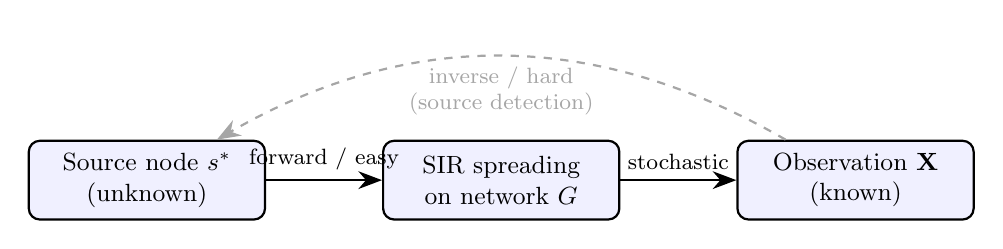
\begin{tikzpicture}[
  box/.style={draw, rounded corners=4pt, minimum width=3cm,
              minimum height=1cm, font=\small, fill=blue!6, thick,
              align=center},
  arr/.style={-{Stealth[length=3mm]}, thick},
  darr/.style={-{Stealth[length=3mm]}, thick, dashed, gray!70}
]

\node[box] (source) at (0,0)   {Source node $s^*$ \\ \small(unknown)};
\node[box] (process) at (4.5,0) {SIR spreading \\ \small on network $G$};
\node[box] (obs)    at (9,0)   {Observation $\mathbf{X}$ \\ \small(known)};

\draw[arr] (source) -- node[above, font=\footnotesize]{forward / easy} (process);
\draw[arr] (process) -- node[above, font=\footnotesize]{stochastic} (obs);

\draw[darr, bend right=30] (obs) to
  node[below, font=\footnotesize, align=center]{inverse / hard \\ (source detection)} (source);

\end{tikzpicture}
\end{center}

The \textbf{forward direction} (left to right) is tractable: given $s^*$ and
$G$, we simulate the SIR process to generate $\mathbf{X}$. This is what the
TSIR engine does.

The \textbf{inverse direction} (right to left) is what we solve in this
thesis: given $\mathbf{X}$ and $G$, recover $s^*$. The arrow is dashed
because the mapping is not a function — the same $\mathbf{X}$ can arise from
multiple different sources, and the same source can produce many different
$\mathbf{X}$ values. The inverse is a probability distribution, not a
deterministic map.

\subsection{What Makes a Source Detectable?}

The following table summarises the structural conditions that make source
detection easier or harder. Each row represents a variable that we
manipulate in the experimental evaluation of Chapter~6.

\begin{conceptbox}{Structural Determinants of Detection Difficulty}
\begin{center}
\renewcommand{\arraystretch}{1.3}
\begin{tabular}{lll}
\toprule
\textbf{Property} & \textbf{Easier detection} & \textbf{Harder detection} \\
\midrule
Network structure     & Tree-like (few cycles)       & Dense (many cycles)        \\
Degree distribution   & Heterogeneous (scale-free)   & Homogeneous (regular, ER)  \\
Observation time $T$  & Early (small $T$)            & Late (large $T$)           \\
Observation coverage  & Full (all nodes)             & Partial (sensor subset)    \\
Temporal resolution   & High (fine timestamps)       & Low (aggregated/static)    \\
Epidemic size $k/N$   & Intermediate                 & Very small or very large   \\
\bottomrule
\end{tabular}
\end{center}
\end{conceptbox}

Each row of this table is a research question. Our experimental setup in
Chapter~6 varies these conditions systematically to understand when and why
different methods succeed or fail.

% ============================================================
\section{Chapter Summary}
\label{sec:source-detection-summary}
% ============================================================

This chapter introduced the source detection problem from the ground up. We
started with the detective analogy and built toward a rigorous mathematical
framework. The key takeaways are:

\begin{enumerate}
    \item \textbf{Source detection is a Bayesian inverse problem.} The
    posterior $P(\text{source}=v \mid \mathbf{X}) \propto
    P(\mathbf{X} \mid \text{source}=v)$ (under a uniform prior) assigns a
    probability to each candidate node.

    \item \textbf{The likelihood is intractable exactly but approximable by
    simulation.} Running $n_{\text{runs}}$ epidemics from each candidate and
    counting matches (exact or soft via Jaccard similarity) gives an unbiased
    estimate.

    \item \textbf{Real observations are noisy and partial.} Soft matching
    and appropriate handling of partial observations are essential for
    robust methods.

    \item \textbf{Four core challenges.} Partial observation, late
    observation, network heterogeneity, and temporal ambiguity each degrade
    detection performance in distinct ways.

    \item \textbf{Evaluation uses rank score and top-$k$ score.} Both
    metrics are normalised to be network-size-independent and are computed
    only on valid test cases via the \texttt{possible} and
    \texttt{maximal\_outbreak} filters.

    \item \textbf{Brute-force MLE is computationally infeasible} for
    networks beyond a few hundred nodes, motivating both classical heuristics
    (Chapter~5) and GNN-based learning methods (Chapters~6--11).
\end{enumerate}

\begin{keyinsight}{The Thesis in One Sentence}
Source detection is a hard inverse problem over a stochastic spreading
process; Graph Neural Networks trained on simulated epidemic data can learn
to approximate the posterior efficiently in a single forward pass, exploiting
both the graph structure and — in temporal architectures — the causal
constraints imposed by contact timestamps.
\end{keyinsight}

\chapter{Classical Source Detection Algorithms}
\label{ch:classical}

\textit{This chapter introduces the four classical algorithms used as baselines in every
source-detection benchmark: a uniform random guesser, a degree-centrality ranker, the
Jordan Center, and Rumor Centrality. Each method encodes a different hypothesis about
what makes a good source candidate. By studying them carefully --- including their
assumptions, their failure modes, and the concrete arithmetic behind them --- you will
build the intuition needed to understand why graph neural networks are a principled
improvement, and what benchmark bar they must clear.}

% ============================================================
\section{Overview: A Map of Classical Methods}
\label{sec:classical-overview}
% ============================================================

Before we commit to any single algorithm, it helps to see the whole landscape at a
glance. The table below compares the four methods along the dimensions that matter most
for a practitioner: how fast they are, whether they even look at the contact network,
and whether any theoretical guarantee backs up their predictions.

\begin{table}[H]
\centering
\caption{Comparison of the four classical source-detection baselines. $N$ = number of
nodes; $|\mathcal{I}|$ = number of infected nodes; $|E_{\mathcal{I}}|$ = edges in the
infected subgraph. The ``Network required?'' column asks whether the method needs the
contact graph or only the compartment labels.}
\label{tab:classical-overview}
\small
\begin{tabular}{lllcc}
\toprule
\textbf{Method} & \textbf{Complexity} & \textbf{Network required?} &
  \textbf{Uses observation?} & \textbf{Theoretical guarantee?} \\
\midrule
Uniform random guess & $O(1)$          & No  & No  & Yes --- lower bound only \\
Degree centrality    & $O(N + |E|)$    & Yes & No  & No                      \\
Jordan Center        & $O(|\mathcal{I}| + |E_{\mathcal{I}}|)$
                                       & Yes & Yes (topology only) & No     \\
Rumor Centrality     & $O(|\mathcal{I}|)$ & Yes & Yes & Yes --- ML on regular trees \\
\bottomrule
\end{tabular}
\end{table}

\begin{conceptbox}{What Is a ``Baseline'' and Why Do We Need One?}
A \textbf{baseline} is the simplest possible algorithm that is still a valid answer to
the problem. It sets the floor: any serious method must beat it, and the gap between
the baseline and a sophisticated method measures how much we have actually learned.

In source detection, the most natural floor is the \textbf{random guesser}: without any
information, pick a node uniformly at random. If your fancy algorithm cannot consistently
beat this, it has learned nothing from the data.

Baselines also act as sanity checks. If a new GNN model scores below the Jordan Center
on every experiment, something is broken --- not in the Jordan Center, but in the
training procedure, the data pipeline, or the model itself. This is precisely why the
\texttt{main\_eval.py} script in this codebase runs all four baselines automatically on
every dataset, logging the results to Weights \& Biases for side-by-side comparison.
\end{conceptbox}

% ============================================================
\section{Baseline 1: Uniform Random Guess}
\label{sec:uniform}
% ============================================================

\subsection{The Idea}

The uniform random guesser assigns the same probability to every node in the network:

\begin{equation}
  P_{\text{uniform}}(v) = \frac{1}{N} \quad \text{for all } v \in V.
  \label{eq:uniform}
\end{equation}

There is no computation, no network traversal, no comparison to the observation. Every
node is equally likely to be the source. This is the ``I have no idea'' algorithm.

\begin{analogybox}{The Lottery Ticket Drawer}
Imagine $N = 100$ lottery tickets in a hat, each bearing the name of one node. The
uniform guesser draws one ticket without looking. The true source wins the draw with
probability $1/100 = 1\%$. There is no skill involved, no information used.

The value of this analogy is that it makes the expected performance concrete. If you
repeat this lottery over many independent epidemics, the true source will be in the
top-1 prediction exactly $1\%$ of the time. Any method that achieves, say, $12\%$
top-1 accuracy has beaten the lottery by a factor of 12 --- a meaningful improvement.
\end{analogybox}

\subsection{The Rank Score Metric}

Before we can compute the ``expected performance'' of any method, we need to agree on
how performance is measured. This workbook uses two metrics extensively.

\textbf{Rank of the true source.} After running an algorithm, rank all $N$ nodes by
their predicted probability (highest = rank 1). The rank of the true source $s^*$
tells us how far down the list we have to go to find the right answer. Rank 1 means
the algorithm got it right; rank $N$ means the true source was dead last.

\textbf{Rank score.} The rank score converts a raw rank $r$ into a number between 0
and 1 where higher is better:

\begin{equation}
  \text{RankScore}(r) = \frac{1}{r}.
  \label{eq:rank-score}
\end{equation}

A rank of 1 gives a score of 1.0 (perfect). A rank of 10 gives 0.1. A rank of 100
gives 0.01. We average this score over all epidemic runs to get a single summary number.

\begin{mathbox}{Expected Rank Score of the Uniform Baseline}
\textbf{Setup.} There are $N$ candidate nodes. The uniform guesser assigns equal
probability $1/N$ to every node, so ties are broken by random shuffling. The true
source ends up in a uniformly random position among the $N$ slots.

\textbf{Expected rank.} Since each of the $N$ positions is equally likely:
\[
  \mathbb{E}[\text{rank}] = \frac{1 + 2 + \cdots + N}{N} = \frac{N+1}{2}.
\]
For $N = 100$: $\mathbb{E}[\text{rank}] = 50.5$.

\textbf{Expected rank score.} By Jensen's inequality, $\mathbb{E}[1/r] \neq 1/\mathbb{E}[r]$.
The exact value requires summing over all positions:
\[
  \mathbb{E}\!\left[\frac{1}{r}\right]
  = \frac{1}{N} \sum_{r=1}^{N} \frac{1}{r}
  = \frac{H_N}{N},
\]
where $H_N = \sum_{r=1}^{N} 1/r$ is the $N$-th harmonic number.

\medskip
\begin{center}
\small
\begin{tabular}{rrrr}
\toprule
$N$ & $\mathbb{E}[\text{rank}]$ & $H_N$ & $\mathbb{E}[\text{RankScore}]$ \\
\midrule
10   & 5.5  & 2.93  & 0.293 \\
50   & 25.5 & 4.50  & 0.090 \\
100  & 50.5 & 5.19  & 0.052 \\
500  & 250.5 & 6.79 & 0.014 \\
\bottomrule
\end{tabular}
\end{center}

\medskip
\textbf{Interpretation.} For $N = 100$ nodes, a method that achieves a mean rank score
above $0.052$ has beaten the random floor. The uniform baseline defines the minimum bar.

\textbf{Important nuance.} In the codebase, not all $N$ nodes are valid source
candidates: the \texttt{possible} binary mask in \texttt{TSIRData} excludes nodes that
could not have started a large enough outbreak given the observed infection size. The
effective pool is therefore often smaller than $N$, raising the uniform floor.
Specifically, if $N_{\text{eff}}$ nodes are in the \texttt{possible} mask, the uniform
baseline assigns probability $1/N_{\text{eff}}$ to each valid candidate and zero to
the rest.
\end{mathbox}

\subsection{Implementation in the Codebase}

The uniform baseline lives in \texttt{eval/benchmark.py}. It is implemented in three
lines:

\begin{codewalk}{Uniform Baseline --- \texttt{eval/benchmark.py}}
\begin{lstlisting}[language=Python]
def uniform_probabilities(possible):
    """
    Assign equal probability to every candidate node.

    Parameters
    ----------
    possible : np.ndarray of shape (n_runs, n_nodes)
        Binary mask; 1 if the node is a valid source candidate.

    Returns
    -------
    np.ndarray of shape (n_runs, n_nodes)
        Probability distribution: 1/N_eff for valid candidates, 0 otherwise.
    """
    return possible / np.sum(possible, axis=1, keepdims=True)
\end{lstlisting}

\textbf{What this does, step by step.}
\begin{enumerate}
  \item \texttt{possible} is a matrix with one row per epidemic run and one column per
        node. A 1 in position $(r, v)$ means node $v$ is a valid candidate for run $r$.
  \item \texttt{np.sum(possible, axis=1, keepdims=True)} counts how many valid
        candidates there are in each run. This is $N_{\text{eff}}$ per run.
  \item Dividing \texttt{possible} by this count spreads probability uniformly across
        valid candidates, leaving zeros for invalid ones.
\end{enumerate}
The function returns a proper probability distribution (all rows sum to 1).
\end{codewalk}

% ============================================================
\section{Baseline 2: Degree Centrality}
\label{sec:degree}
% ============================================================

\subsection{The Idea and Its Justification}

The degree of a node $v$ in an undirected network is the number of edges incident to it:

\begin{equation}
  \deg(v) = |\{u \in V : (u, v) \in E\}|.
  \label{eq:degree}
\end{equation}

The degree-centrality heuristic ranks nodes by their degree and predicts the
highest-degree node as the most likely source:

\begin{equation}
  \hat{s}_{\text{degree}} = \arg\max_{v \in V} \deg(v).
  \label{eq:degree-heuristic}
\end{equation}

\textbf{Why might this work?} A node with many connections --- a \textbf{hub} ---
contacts more people per unit time than a peripheral node. During an epidemic, a hub
that becomes infected early will, on average, infect more neighbours sooner, producing
a larger and more centrally-located outbreak. If we observe a large outbreak and
try to guess where it started, the hub is a rational first suspect.

\begin{analogybox}{The Well-Connected Person at a Party}
Imagine you arrive at a party where 30 out of 100 guests have already come down with
norovirus. You need to identify Patient Zero. You know nothing about who interacted
with whom during the illness, but you do know the social structure: some people talked
to almost everyone (the extroverts, high degree), and some barely spoke to anyone
(the wallflowers, low degree).

The degree heuristic says: blame the extrovert first. On average, a highly connected
person is more likely to have spread the infection to so many people. This is a
reasonable prior, but it ignores the actual infection pattern. Maybe the wallflower
was the first to get sick, and the extrovert caught it from them.
\end{analogybox}

\subsection{Worked Example on a 5-Node Graph}

\begin{examplebox}{Degree Centrality on a 5-Node Network}
\textbf{Graph.} Five nodes $\{v_1, v_2, v_3, v_4, v_5\}$ with the following edges:
$(v_1, v_2)$, $(v_1, v_3)$, $(v_1, v_4)$, $(v_2, v_3)$, $(v_3, v_5)$.

\begin{center}
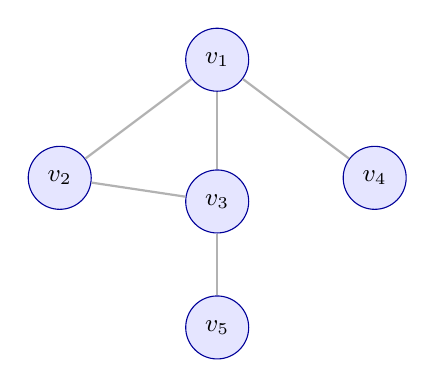
\begin{tikzpicture}[
  nd/.style={circle, draw=blue!60!black, fill=blue!10, minimum size=0.8cm,
             font=\small\bfseries},
  inf/.style={circle, draw=red!60!black, fill=red!15, minimum size=0.8cm,
              font=\small\bfseries},
  edge/.style={thick, gray!60}
]
  \node[nd] (v1) at (0, 0)    {$v_1$};
  \node[nd] (v2) at (-2, -1.5){$v_2$};
  \node[nd] (v3) at (0, -1.8) {$v_3$};
  \node[nd] (v4) at (2, -1.5) {$v_4$};
  \node[nd] (v5) at (0, -3.4) {$v_5$};

  \draw[edge] (v1) -- (v2);
  \draw[edge] (v1) -- (v3);
  \draw[edge] (v1) -- (v4);
  \draw[edge] (v2) -- (v3);
  \draw[edge] (v3) -- (v5);
\end{tikzpicture}
\end{center}

\textbf{Step 1: Compute degrees.}
\begin{center}
\small
\begin{tabular}{lcc}
\toprule
Node & Neighbours & Degree \\
\midrule
$v_1$ & $v_2, v_3, v_4$ & 3 \\
$v_2$ & $v_1, v_3$       & 2 \\
$v_3$ & $v_1, v_2, v_5$  & 3 \\
$v_4$ & $v_1$            & 1 \\
$v_5$ & $v_3$            & 1 \\
\bottomrule
\end{tabular}
\end{center}

\textbf{Step 2: Rank by degree (ties broken randomly).}
$v_1$ and $v_3$ both have degree 3. One is ranked first, the other second.

\textbf{Step 3: The prediction.} The degree heuristic predicts either $v_1$ or $v_3$
as the source (a coin flip between the two).

\textbf{Scenario A: True source is $v_1$.} Degree heuristic is correct 50\% of the
time (when $v_1$ wins the tie-break). Top-2 accuracy is 100\%.

\textbf{Scenario B: True source is $v_4$.} Degree heuristic predicts $v_1$ or $v_3$
(both wrong). The true source $v_4$ has the lowest degree (degree 1). The algorithm
fails completely --- it is farthest from the right answer.

\textbf{Takeaway.} Degree centrality is a useful prior on hub-seeded outbreaks but is
systematically wrong when the true source is peripheral.
\end{examplebox}

\subsection{The Critical Limitation: Blindness to the Observation}

The most important weakness of degree centrality is that it does not look at
\textit{who is actually infected}. Consider two scenarios:

\begin{enumerate}
  \item \textbf{Hub-initiated outbreak.} Node $v_1$ (degree 10) starts the epidemic.
        After $T = 5$ steps, its 10 direct neighbours are all infected. The degree
        heuristic correctly ranks $v_1$ first.

  \item \textbf{Peripheral-node outbreak.} Node $v_{99}$ (degree 1) starts the
        epidemic. By coincidence, it is connected to the hub, which then spreads the
        infection widely. The degree heuristic ranks $v_{99}$ last --- completely wrong.
\end{enumerate}

In both scenarios, the degree heuristic produces the identical ranking. It is
``observation-blind'': the actual pattern of infection carries zero weight in its
prediction.

\begin{keyinsight}{Degree Centrality as a Prior, Not a Likelihood}
In Bayesian language, degree centrality is a \textbf{prior}: it encodes our belief
about which nodes are likely sources \emph{before we observe the epidemic}. On
scale-free networks (where hubs are disproportionately common), this prior is
informative. But a good inference algorithm should update this prior with the
\textbf{likelihood} of the observed infection pattern given each candidate source.

The Jordan Center and Rumor Centrality (sections below) take a first step in this
direction: they ask not just ``who is likely to have started it?'' but ``given the
pattern I see, which node is most consistent with being the origin?''
\end{keyinsight}

% ============================================================
\section{Baseline 3: Jordan Center}
\label{sec:jordan}
% ============================================================

\subsection{Motivation: The Source Is Near the Center}

When a disease starts at node $s$ and spreads outward, the infected subgraph grows
like a ripple in a pond: the source is at the center, and the infection front is at
the periphery. At any observation time $T$, the infected nodes form a connected (or
nearly connected) subgraph, and the source is located somewhere near the geometric
center of that subgraph.

This geometric intuition motivates the \textbf{Jordan Center}: find the node that is
closest to all other infected nodes simultaneously --- the node that minimises the
maximum distance to any other infected node.

\begin{conceptbox}{Key Definitions: Distance, Eccentricity, and Jordan Center}
Let $\mathcal{I} \subseteq V$ denote the set of infected (I or R) nodes at observation
time $T$. Let $G_{\mathcal{I}}$ be the subgraph induced by $\mathcal{I}$.

\medskip
\textbf{Shortest-path distance.} The distance $d(u, v)$ between two nodes $u, v \in
\mathcal{I}$ is the number of edges on the shortest path between them in
$G_{\mathcal{I}}$.

\medskip
\textbf{Eccentricity.} The eccentricity of a node $v \in \mathcal{I}$ is:
\begin{equation}
  \text{ecc}(v) = \max_{u \in \mathcal{I}} d(v, u).
  \label{eq:eccentricity}
\end{equation}
The eccentricity measures how far the most distant infected node is from $v$. A small
eccentricity means $v$ is ``centrally located'' within the infected subgraph.

\medskip
\textbf{Jordan Center.} The Jordan Center is the node (or set of nodes) with minimum
eccentricity within the infected subgraph:
\begin{equation}
  \hat{s}_{\text{Jordan}} = \arg\min_{v \in \mathcal{I}} \text{ecc}(v).
  \label{eq:jordan}
\end{equation}
This is also known as the \textbf{graph center} or \textbf{$1$-center} of the induced
subgraph.
\end{conceptbox}

\subsection{Step-by-Step Example on a 6-Node Infected Subgraph}

\begin{examplebox}{Jordan Center Computation on a 6-Node Subgraph}
\textbf{Setup.} Six infected nodes $\{A, B, C, D, E, F\}$ with edges:
$(A,B)$, $(B,C)$, $(C,D)$, $(C,E)$, $(E,F)$.

\textbf{Graph layout (draw it):}
\begin{center}
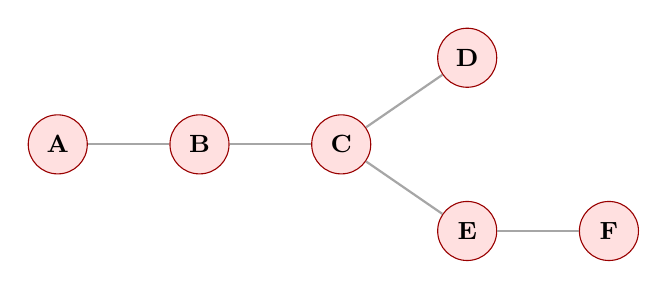
\begin{tikzpicture}[
  nd/.style={circle, draw=red!60!black, fill=red!12, minimum size=0.75cm,
             font=\small\bfseries},
  edge/.style={thick, gray!70}
]
  \node[nd] (A) at (0, 0)   {A};
  \node[nd] (B) at (1.8, 0) {B};
  \node[nd] (C) at (3.6, 0) {C};
  \node[nd] (D) at (5.2, 1.1) {D};
  \node[nd] (E) at (5.2, -1.1){E};
  \node[nd] (F) at (7.0, -1.1){F};

  \draw[edge] (A) -- (B);
  \draw[edge] (B) -- (C);
  \draw[edge] (C) -- (D);
  \draw[edge] (C) -- (E);
  \draw[edge] (E) -- (F);
\end{tikzpicture}
\end{center}

\textbf{Step 1: Compute all pairwise shortest-path distances (BFS from each node).}

\begin{center}
\small
\begin{tabular}{lcccccc}
\toprule
$d(\cdot, \cdot)$ & A & B & C & D & E & F \\
\midrule
A & 0 & 1 & 2 & 3 & 3 & 4 \\
B & 1 & 0 & 1 & 2 & 2 & 3 \\
C & 2 & 1 & 0 & 1 & 1 & 2 \\
D & 3 & 2 & 1 & 0 & 2 & 3 \\
E & 3 & 2 & 1 & 2 & 0 & 1 \\
F & 4 & 3 & 2 & 3 & 1 & 0 \\
\bottomrule
\end{tabular}
\end{center}

\textbf{Step 2: Compute eccentricity for each node} (maximum in its row above).

\begin{center}
\small
\begin{tabular}{lcc}
\toprule
Node & $\max_u d(v, u)$ & Eccentricity \\
\midrule
A & $\max(0,1,2,3,3,4) = 4$ & 4 \\
B & $\max(1,0,1,2,2,3) = 3$ & 3 \\
C & $\max(2,1,0,1,1,2) = 2$ & \textbf{2} \\
D & $\max(3,2,1,0,2,3) = 3$ & 3 \\
E & $\max(3,2,1,2,0,1) = 3$ & 3 \\
F & $\max(4,3,2,3,1,0) = 4$ & 4 \\
\bottomrule
\end{tabular}
\end{center}

\textbf{Step 3: Identify the Jordan Center.}
The minimum eccentricity is 2, achieved uniquely by node $C$.

$\hat{s}_{\text{Jordan}} = C$.

\textbf{Interpretation.} Node $C$ is the most ``central'' node in the infected
subgraph in the sense that even its farthest infected neighbour (nodes $A$ or $F$) is
only 2 hops away. Any other node has at least one infected node at distance 3 or 4.

\textbf{Is the prediction correct?} If the true source is $C$, yes. If the epidemic
actually started at $B$ (which is also fairly central), the Jordan Center gives rank 2
--- still a good prediction.
\end{examplebox}

\subsection{Algorithm Pseudocode}

\begin{codewalk}{Jordan Center --- Pseudocode}
\begin{lstlisting}[language=Python]
from collections import deque

def jordan_center(infected_nodes: list[int],
                  adjacency: dict[int, list[int]]) -> int:
    """
    Find the Jordan Center of the infected subgraph.

    Parameters
    ----------
    infected_nodes : list of node indices in state I or R
    adjacency      : adjacency list of the FULL network
                     (we use only edges within infected_nodes)

    Returns
    -------
    int : node index of the Jordan Center
    """
    infected_set = set(infected_nodes)

    def bfs_eccentricity(source: int) -> int:
        """BFS within infected subgraph; return max distance."""
        dist = {source: 0}
        queue = deque([source])
        max_dist = 0
        while queue:
            v = queue.popleft()
            for u in adjacency[v]:
                if u in infected_set and u not in dist:
                    dist[u] = dist[v] + 1
                    max_dist = max(max_dist, dist[u])
                    queue.append(u)
        return max_dist

    # Compute eccentricity for every infected node
    eccentricities = {v: bfs_eccentricity(v) for v in infected_nodes}

    # Return the node with minimum eccentricity (ties broken by index)
    return min(eccentricities, key=lambda v: eccentricities[v])
\end{lstlisting}

\textbf{Complexity analysis.}
BFS from a single source in a subgraph of $|\mathcal{I}|$ nodes and $|E_\mathcal{I}|$
edges runs in $O(|\mathcal{I}| + |E_\mathcal{I}|)$. We run one BFS per infected node,
giving total complexity $O(|\mathcal{I}| \cdot (|\mathcal{I}| + |E_\mathcal{I}|))$.

\textbf{Practical note.} On very sparse trees, this can be sped up to $O(|\mathcal{I}|)$
using the double-BFS diameter algorithm, but the naive version above is clear and
correct for all graph types.
\end{codewalk}

\subsection{Why the Jordan Center Works (and When It Fails)}

\begin{keyinsight}{The Uniform-Speed Assumption Behind the Jordan Center}
The Jordan Center is optimal if and only if the epidemic spreads at a \textbf{uniform
speed} in all directions. Formally, if each edge transmits the infection in exactly one
time step and recovery takes a fixed time, then after $T$ steps the infected subgraph
is a ``ball'' of radius $T$ around the source in the contact network. The source is
the center of this ball, which is exactly the Jordan Center.

\medskip
\textbf{When this breaks down:}
\begin{enumerate}
  \item \textbf{Heterogeneous contact rates.} If some edges are traversed more
        frequently (temporal networks with bursty contacts), the ball is distorted ---
        the infection reaches some directions faster than others. The geometric center
        of the infected subgraph is no longer the source.
  \item \textbf{Dense subgraphs and shortcuts.} If the infected subgraph contains
        dense clusters or highly connected hubs, the shortest-path distances within the
        subgraph do not reflect the diffusion dynamics. A peripheral source inside a
        dense cluster may produce short eccentricity due to the cluster's diameter.
  \item \textbf{Incomplete observation.} If only a fraction of infected nodes are
        observed (e.g., asymptomatic cases go undetected), the observed subgraph may
        have a geometric center far from the true source.
\end{enumerate}

\medskip
\textbf{Empirical performance.} Despite these limitations, the Jordan Center is
surprisingly competitive on real-world contact networks \cite{Sterchi2025}, often
outperforming more complex analytical methods on sparse, tree-like topologies. This is
why it serves as the primary structural baseline in the experimental evaluation of
Chapter~\ref{ch:classical}.
\end{keyinsight}

% ============================================================
\section{Baseline 4: Rumor Centrality (Shah \& Zaman, 2011)}
\label{sec:rumor}
% ============================================================

\subsection{Motivation: Counting Infection Orderings}

The three methods above either ignore the observation entirely (uniform, degree) or
use only the geometry of the infected subgraph (Jordan Center). Rumor Centrality goes
one step deeper: it asks a combinatorial question about the \textit{spreading process
itself}.

Suppose the contact graph were a tree and the epidemic were an SI process (no recovery)
with equal transmission probability on every edge. In this ideal world, the infection
spreads in a random order, visiting each node exactly once. There are many possible
orderings: perhaps $v_1$ infected $v_2$ before $v_3$, or perhaps in the reverse order.

\textbf{The key question:} For a given observation (all nodes infected, i.e., the full
tree), which node $v$ has the maximum number of distinct orderings --- ``infection
permutations'' --- that lead to the final state?

The answer is the \textbf{Rumor Center}: the node that maximises the count of valid
spreading orderings. Shah \& Zaman proved in 2011 that this is the Maximum Likelihood
Estimator (MLE) for the source on a regular tree under the SI model
\cite{Shah2011}.

\begin{analogybox}{Counting Ways the Story Could Have Unfolded}
Think of the infection as a rumor spreading through a group of friends arranged in a
tree-shaped friendship network. The rumor starts with one person and spreads outward.
By the time everyone has heard it, there are many possible orderings of who told whom
first.

Person A (at the center of the tree) could have told their story in many sequences
--- first to the left branch, then the right, interleaving freely. Person B (at a
leaf) had fewer choices: they could only have heard the rumor after their one friend
told them, and they could not have spread it further before hearing it.

Rumor Centrality counts, for each candidate ``first teller,'' how many valid orderings
could have led to everyone knowing the rumor. The person who maximises this count is
the most plausible originator.
\end{analogybox}

\subsection{Formal Definition}

Let $T = (V, E)$ be a tree with $N$ nodes. Fix a candidate root $v$. When we root the
tree at $v$, every other node $u$ becomes the root of a subtree. Define:

\begin{equation}
  T_u(v) = \text{size of the subtree rooted at } u \text{ when the tree is rooted at } v.
  \label{eq:subtree-size}
\end{equation}

By convention, $T_v(v) = N$ (the whole tree is the subtree of the root itself).

\begin{mathbox}{Rumor Centrality: Definition and Recursion}
\textbf{Definition.} The Rumor Centrality of node $v$ on a tree with $N$ infected
nodes is:
\begin{equation}
  R(v) = \frac{N!}{\prod_{u \in V} T_u(v)}.
  \label{eq:rumor}
\end{equation}

\textbf{Interpretation.} $N!$ is the total number of orderings of $N$ nodes. Dividing
by the product of subtree sizes counts the fraction of those orderings that are
consistent with $v$ being the source --- orderings where the infection reached every
subtree in a valid causal sequence.

\textbf{Efficient computation via the subtree-size recursion.}
Computing $T_u(v)$ for all $u$ by rerooting naively would take $O(N^2)$ time.
A two-pass dynamic programming algorithm runs in $O(N)$:

\textit{Pass 1 (upward):} Root the tree arbitrarily at $v$. Compute subtree sizes
bottom-up:
\[
  T_u(v) = 1 + \sum_{\text{children } c \text{ of } u} T_c(v).
\]

\textit{Relative update (re-rooting):} When we move the root from $v$ to a neighbour
$w$, only two subtree sizes change:
\[
  T_w(w) = N, \quad T_v(w) = N - T_w(v).
\]
All other subtree sizes are unchanged. This allows computing $R(w)$ from $R(v)$ in
$O(1)$:
\begin{equation}
  R(w) = R(v) \cdot \frac{T_w(v)}{N - T_w(v)}.
  \label{eq:rumor-update}
\end{equation}

\textbf{Full algorithm.} Pick any starting node; compute $R(v)$ by Pass 1. Then
propagate Eq.~(\ref{eq:rumor-update}) over a DFS/BFS traversal of the tree. Total
complexity: $O(N)$.
\end{mathbox}

\subsection{Worked Example on a 5-Node Tree}

\begin{examplebox}{Rumor Centrality on a 5-Node Tree}
\textbf{Tree.} Five nodes $\{1, 2, 3, 4, 5\}$ with edges:
$(1,2)$, $(2,3)$, $(3,4)$, $(3,5)$.

\begin{center}
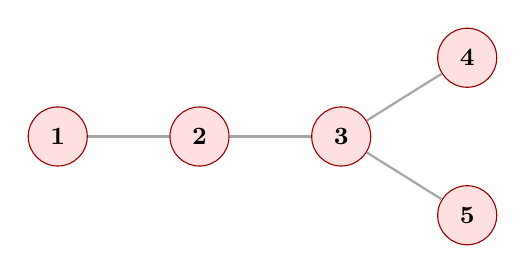
\begin{tikzpicture}[
  nd/.style={circle, draw=red!60!black, fill=red!12, minimum size=0.75cm,
             font=\small\bfseries},
  edge/.style={thick, gray!70}
]
  \node[nd] (n1) at (0, 0)    {1};
  \node[nd] (n2) at (1.8, 0)  {2};
  \node[nd] (n3) at (3.6, 0)  {3};
  \node[nd] (n4) at (5.2, 1.0){4};
  \node[nd] (n5) at (5.2,-1.0){5};

  \draw[edge] (n1) -- (n2);
  \draw[edge] (n2) -- (n3);
  \draw[edge] (n3) -- (n4);
  \draw[edge] (n3) -- (n5);
\end{tikzpicture}
\end{center}

There are $N = 5$ nodes, so $N! = 120$.

\medskip
\textbf{Step 1: Root at each candidate and compute subtree sizes $T_u(v)$.}

\medskip
\textbf{Root at $v = 1$:}
\begin{center}
\small
\begin{tabular}{lll}
\toprule
Node $u$ & Children of $u$ (rooted at 1) & $T_u(1)$ \\
\midrule
1 & \{2\}     & 5 (whole tree) \\
2 & \{3\}     & 4 \\
3 & \{4, 5\}  & 3 \\
4 & $\emptyset$ & 1 \\
5 & $\emptyset$ & 1 \\
\bottomrule
\end{tabular}
\end{center}
$R(1) = \dfrac{120}{5 \cdot 4 \cdot 3 \cdot 1 \cdot 1} = \dfrac{120}{60} = 2$.

\medskip
\textbf{Root at $v = 2$:}
When we move the root from 1 to 2, node 1's subtree size becomes $5 - T_2(1) = 5 - 4 = 1$.
All others remain.
\begin{center}
\small
\begin{tabular}{ll}
\toprule
Node $u$ & $T_u(2)$ \\
\midrule
2 & 5 \\
1 & 1 \\
3 & 3 \\
4 & 1 \\
5 & 1 \\
\bottomrule
\end{tabular}
\end{center}
$R(2) = \dfrac{120}{5 \cdot 1 \cdot 3 \cdot 1 \cdot 1} = \dfrac{120}{15} = 8$.

\medskip
\textbf{Root at $v = 3$:}
\begin{center}
\small
\begin{tabular}{ll}
\toprule
Node $u$ & $T_u(3)$ \\
\midrule
3 & 5 \\
2 & 2 \quad (subtree: $\{1, 2\}$) \\
1 & 1 \\
4 & 1 \\
5 & 1 \\
\bottomrule
\end{tabular}
\end{center}
$R(3) = \dfrac{120}{5 \cdot 2 \cdot 1 \cdot 1 \cdot 1} = \dfrac{120}{10} = 12$.

\medskip
\textbf{Root at $v = 4$:}
By symmetry with node 5 (and using the update formula from node 3):
$T_4(4) = 5,\; T_3(4) = 4,\; T_2(4) = 2,\; T_1(4) = 1,\; T_5(4) = 1$.

$R(4) = \dfrac{120}{5 \cdot 4 \cdot 2 \cdot 1 \cdot 1} = \dfrac{120}{40} = 3$.

\textbf{Root at $v = 5$:} Identical to $v = 4$ by symmetry. $R(5) = 3$.

\medskip
\textbf{Step 2: Summary and prediction.}
\begin{center}
\small
\begin{tabular}{lcc}
\toprule
Candidate $v$ & $R(v)$ & Rank \\
\midrule
3 & 12 & \textbf{1} \\
2 & 8  & 2 \\
4 & 3  & 3 \\
5 & 3  & 4 \\
1 & 2  & 5 \\
\bottomrule
\end{tabular}
\end{center}

The Rumor Centrality predicts node 3 as the source. This is the node at the structural
center of the tree (connecting the two branches), which accords with the geometric
intuition. On regular trees, this is provably the MLE.
\end{examplebox}

\subsection{Why Rumor Centrality Fails on Temporal Networks}

Rumor Centrality was derived under a set of idealised assumptions. Understanding these
assumptions makes it clear why the method is not directly applicable to temporal
contact networks.

\begin{keyinsight}{The Three Assumptions That Limit Rumor Centrality}
\textbf{Assumption 1: Static tree structure.}
The derivation requires that the contact graph is a \emph{tree} (no cycles). On a
general graph with cycles, the product $\prod_u T_u(v)$ no longer enumerates spreading
orderings correctly, because cycles allow infection to arrive via multiple paths, which
the formula does not account for.

\textbf{Assumption 2: SI dynamics (no recovery).}
The counting argument assumes every node eventually gets infected ($R(v)$ counts
orderings over all $N$ nodes). Under the SIR model, some nodes recover before
infecting their neighbours and are not in the final infected set. The formula breaks
down because the infected set is not the full tree.

\textbf{Assumption 3: Uniform, memoryless transmission.}
The derivation assumes every edge has the same transmission probability and that each
contact has an equal chance of transmitting, regardless of \emph{when} it occurred.
In a temporal contact network, some contacts happen before others, creating a causal
ordering that is invisible to Rumor Centrality. A contact at time $t=1$ can only
transmit if the infector was already infected at $t=1$; Rumor Centrality ignores this.

\medskip
\textbf{Consequence for this thesis.} None of the contact networks we study (temporal
networks with event timestamps) satisfy these assumptions. We use Rumor Centrality as
an upper bound on what a ``static structural'' approach can achieve --- its performance
tells us how much signal exists in the topology alone, ignoring timing. The GNN
architectures in Parts IV and V are designed to exploit temporal information that
Rumor Centrality discards.
\end{keyinsight}

% ============================================================
\section{Comparing All Four Methods on a Worked Example}
\label{sec:classical-comparison}
% ============================================================

\begin{examplebox}{All Four Methods on a Single Epidemic}
\textbf{Setup.} A 6-node network with 8 temporal contact events. Nodes are labelled
$\{1, 2, 3, 4, 5, 6\}$. The static projection (aggregate of all contacts) has edges:
$(1,2)$, $(1,3)$, $(2,4)$, $(3,4)$, $(3,5)$, $(4,6)$.

The eight temporal events, in order, are:
\begin{center}
\small
\begin{tabular}{lcc}
\toprule
Event & Edge & Time \\
\midrule
1 & $(3, 5)$ & $t = 1$ \\
2 & $(1, 3)$ & $t = 2$ \\
3 & $(1, 2)$ & $t = 3$ \\
4 & $(3, 4)$ & $t = 4$ \\
5 & $(2, 4)$ & $t = 5$ \\
6 & $(4, 6)$ & $t = 6$ \\
7 & $(1, 3)$ & $t = 7$ \\
8 & $(3, 5)$ & $t = 8$ \\
\bottomrule
\end{tabular}
\end{center}

\textbf{Epidemic.} The epidemic starts at node $s^* = 3$ at $t = 0$ with parameters
$\beta = 0.8$, $\mu = 0.1$. After running the SIR process, the observation at $T = 8$
is:
\begin{center}
\small
\begin{tabular}{lcc}
\toprule
Node & State at $T=8$ & Interpretation \\
\midrule
1 & R & Infected then recovered \\
2 & R & Infected then recovered \\
3 & R & True source, recovered \\
4 & R & Infected then recovered \\
5 & I & Still infectious \\
6 & S & Never infected \\
\bottomrule
\end{tabular}
\end{center}

Infected/recovered set: $\mathcal{I} = \{1, 2, 3, 4, 5\}$ (node 6 stayed susceptible).

\medskip
\textbf{Method 1 — Uniform Random Guess.}
Assign probability $1/6$ to each node. The true source 3 is in a uniformly random
position; on average it gets rank $3.5$ out of 6. Expected rank score $\approx 0.41$.

\medskip
\textbf{Method 2 — Degree Centrality.}
Compute degrees from the static projection:
\begin{center}
\small
\begin{tabular}{llc}
\toprule
Node & Neighbours & Degree \\
\midrule
1 & 2, 3     & 2 \\
2 & 1, 4     & 2 \\
3 & 1, 4, 5  & 3 \\
4 & 2, 3, 6  & 3 \\
5 & 3        & 1 \\
6 & 4        & 1 \\
\bottomrule
\end{tabular}
\end{center}

Nodes 3 and 4 tie for the top position (degree 3). The true source (node 3) is
predicted with 50\% probability. \textbf{Expected rank: 1.5 out of 6.} This is better
than uniform because the true source happens to be a hub in this example.

\medskip
\textbf{Method 3 — Jordan Center.}
The infected subgraph $G_\mathcal{I}$ has nodes $\{1, 2, 3, 4, 5\}$ and edges
(from the static projection): $(1,2)$, $(1,3)$, $(2,4)$, $(3,4)$, $(3,5)$.

Pairwise distances within $G_\mathcal{I}$ (by inspection or BFS):
\begin{center}
\small
\begin{tabular}{lrrrrr}
\toprule
$d(\cdot,\cdot)$ & 1 & 2 & 3 & 4 & 5 \\
\midrule
1 & 0 & 1 & 1 & 2 & 2 \\
2 & 1 & 0 & 2 & 1 & 3 \\
3 & 1 & 2 & 0 & 1 & 1 \\
4 & 2 & 1 & 1 & 0 & 2 \\
5 & 2 & 3 & 1 & 2 & 0 \\
\bottomrule
\end{tabular}
\end{center}

Eccentricities: $\text{ecc}(1) = 2$, $\text{ecc}(2) = 3$, $\text{ecc}(3) = 2$,
$\text{ecc}(4) = 2$, $\text{ecc}(5) = 3$.

Minimum eccentricity is 2, achieved by nodes 1, 3, and 4. The true source (node 3) is
among the three Jordan Center nodes. \textbf{Rank: 1, 2, or 3 (uniformly, among the
tied nodes); expected rank $\approx 2$. }

\medskip
\textbf{Method 4 — Rumor Centrality.}
Compute $R(v)$ for each node using the tree formed by the infected subgraph. The
infected subgraph has a cycle: $(1,2), (2,4), (4,3), (3,1)$ form a 4-cycle. Strictly,
Rumor Centrality requires a tree, so we note this as a limitation. Applying the formula
to the spanning tree $\{(1,3), (3,4), (4,2), (3,5)\}$ (BFS tree rooted at node 3):

$T_u(3)$ for each node: $T_3 = 5$, $T_1 = 1$, $T_4 = 2$, $T_2 = 1$, $T_5 = 1$.

$R(3) = \dfrac{5!}{5 \cdot 1 \cdot 2 \cdot 1 \cdot 1} = \dfrac{120}{10} = 12$.

Repeating for other candidates (not shown for brevity): node 3 achieves the highest
Rumor Centrality. \textbf{Prediction: node 3. Rank: 1.}

\medskip
\textbf{Summary.}
\begin{center}
\small
\begin{tabular}{llcc}
\toprule
Method & Prediction & Rank of true source (node 3) & Rank Score \\
\midrule
Uniform random & Random & 3.5 (expected) & 0.41 (expected) \\
Degree centrality & 3 or 4 (tie) & 1.5 (expected) & 0.67 (expected) \\
Jordan Center & 1, 3, or 4 (tie) & 2.0 (expected) & 0.50 (expected) \\
Rumor Centrality & 3 & 1 & 1.00 \\
\bottomrule
\end{tabular}
\end{center}

In this particular example, Rumor Centrality wins because the infected subgraph is
approximately tree-like and the source is the structural center. In practice, across
thousands of epidemic runs on irregular temporal networks, no single classical method
dominates; their relative performance depends on network topology, epidemic size, and
observation time.
\end{examplebox}

\begin{conceptbox}{What This Comparison Teaches Us}
This single worked example illustrates a broader pattern visible in every empirical
benchmark:

\begin{enumerate}
  \item \textbf{Structural methods outperform random guessing by a wide margin.} Even
        degree centrality and the Jordan Center, which ignore or simplify the epidemic
        dynamics, dramatically reduce the effective search space.

  \item \textbf{No classical method systematically dominates.} Degree centrality wins
        on hub-seeded outbreaks; the Jordan Center wins when the infected subgraph is
        a clean ``ball''; Rumor Centrality wins on tree-like topologies with SI
        dynamics. Each method embeds a specific assumption, and real epidemics violate
        all of them.

  \item \textbf{The temporal signal is completely unused.} None of the four methods
        uses the timestamps of contact events. A method that correctly reasons about
        causal ordering --- which contacts happened before which, and which paths are
        therefore temporally feasible --- can do substantially better. This is the core
        motivation for the temporal GNN architectures in this thesis.
\end{enumerate}
\end{conceptbox}

% ============================================================
\section{Implementation in the Codebase}
\label{sec:classical-code}
% ============================================================

The codebase implements the uniform baseline analytically and the structural baselines
(degree and Jordan Center) as functions operating on the \texttt{TSIRData} dataclass
produced by \texttt{main\_tsir.py}.

\subsection{How the Evaluation Pipeline Works}

\begin{conceptbox}{The \texttt{main\_eval.py} Pipeline}
The script \texttt{main\_eval.py} automates the following steps for every baseline:

\begin{enumerate}
  \item \textbf{Load the artifact.} The script reads a \texttt{TSIRData} artifact from
        Weights \& Biases (logged during the data generation step in
        \texttt{main\_tsir.py}). This artifact contains ground-truth source labels,
        Monte Carlo simulation results, the contact network, and the \texttt{possible}
        mask.

  \item \textbf{Run the baseline.} For each epidemic run, the baseline produces a
        probability vector $p \in \mathbb{R}^N$ over nodes.

  \item \textbf{Compute metrics.} The \texttt{eval/scores.py} and
        \texttt{eval/ranks.py} modules compute rank scores, top-$k$ accuracy, and
        other metrics defined in Section~\ref{sec:classical-overview}.

  \item \textbf{Log to wandb.} All metrics are pushed to the
        \texttt{source-detection} project in Weights \& Biases for side-by-side
        comparison with GNN models.
\end{enumerate}

The \texttt{possible} mask is critical: it restricts scoring to epidemic runs where
a sufficiently large outbreak occurred and the source node is plausibly identifiable.
Without this filter, trivially small outbreaks (where only the source itself is
infected) inflate the performance of every method.
\end{conceptbox}

\subsection{Uniform Baseline}

\begin{codewalk}{Uniform Baseline in \texttt{eval/benchmark.py}}
\begin{lstlisting}[language=Python]
import numpy as np

def uniform_probabilities(possible: np.ndarray) -> np.ndarray:
    """
    Assign equal probability to every valid source candidate.

    Parameters
    ----------
    possible : np.ndarray, shape (n_nodes * n_runs, n_nodes)
        Binary mask. Row i contains 1s for all nodes that are valid
        source candidates for run i.

    Returns
    -------
    np.ndarray, shape (n_nodes * n_runs, n_nodes)
        Row-normalised probability matrix.
    """
    return possible / np.sum(possible, axis=1, keepdims=True)
\end{lstlisting}
\end{codewalk}

\subsection{Rank Score and Top-k Metrics}

Both metrics are implemented in \texttt{eval/scores.py}:

\begin{codewalk}{Scoring Functions in \texttt{eval/scores.py}}
\begin{lstlisting}[language=Python]
import numpy as np

def rank_score(ranks: np.ndarray, sel: np.ndarray,
               offset: float = 0) -> float:
    """
    Compute mean 1/rank over selected runs.

    Parameters
    ----------
    ranks  : array of source ranks (1 = best)
    sel    : boolean mask selecting which runs to include
    offset : optional smoothing offset (rarely used)
    """
    return np.mean((1 + offset) / (ranks[sel] + offset))


def top_k_score(ranks: np.ndarray, sel: np.ndarray,
                k: int = 5) -> float:
    """
    Fraction of selected runs where the true source is in the top-k.
    """
    return np.mean(ranks[sel] <= k)
\end{lstlisting}

\textbf{How ranks are computed.} The companion function in \texttt{eval/ranks.py}
takes the raw probability vectors from any baseline or GNN model and converts them
into integer ranks:

\begin{lstlisting}[language=Python]
def compute_expected_ranks(values: np.ndarray,
                           n_nodes: int,
                           n_runs: int) -> np.ndarray:
    """
    For each (source, run) pair, compute the rank of the true source.

    The rank of the true source is: (number of nodes with strictly
    higher predicted probability) + (number of ties + 1) / 2.
    This handles ties symmetrically.
    """
    # Index the predicted value of the true source for each run
    source_values = values[
        np.arange(n_nodes * n_runs),
        np.repeat(np.arange(n_nodes), n_runs)
    ]
    # Number of nodes strictly better than the true source
    rank = np.sum(values > source_values[:, None], axis=1)
    # Add half the ties (expected rank under random tie-breaking)
    ties = np.sum(values == source_values[:, None], axis=1)
    rank = rank + (ties + 1) / 2
    return rank
\end{lstlisting}

\textbf{Worked example.} Suppose $N = 4$ nodes and predicted probabilities for one run
are $[0.4, 0.3, 0.2, 0.1]$, and the true source is node 3 (probability 0.2). Then:
\begin{itemize}
  \item Nodes with strictly higher probability: nodes 1 and 2 $\Rightarrow$ count = 2.
  \item Nodes with equal probability: just node 3 itself $\Rightarrow$ ties = 1.
  \item Expected rank = $2 + (1 + 1)/2 = 3$.
\end{itemize}
The true source gets rank 3 out of 4 in this run, giving a rank score of $1/3 \approx 0.33$.
\end{codewalk}

\subsection{Putting It Together: What to Expect from Each Baseline}

\begin{keyinsight}{Expected Benchmark Performance of Classical Methods}
Based on the theoretical analysis and the empirical literature \cite{Sterchi2025},
here is what you should expect when running \texttt{main\_eval.py} on a moderately
sized Erd\H{o}s-R\'{e}nyi network ($N = 100$, mean degree $\approx 6$, $\beta = 0.3$):

\begin{center}
\small
\begin{tabular}{lcc}
\toprule
Method & Expected mean rank score & Expected top-5 accuracy \\
\midrule
Uniform random    & $\approx 0.05$  & $\approx 5\%$  \\
Degree centrality & $\approx 0.10$--$0.15$ & $\approx 10\%$--$20\%$ \\
Jordan Center     & $\approx 0.15$--$0.25$ & $\approx 20\%$--$35\%$ \\
Rumor Centrality  & $\approx 0.20$--$0.30$ & $\approx 25\%$--$40\%$ \\
\bottomrule
\end{tabular}
\end{center}

These numbers vary substantially with network topology, epidemic size, and observation
time. The important point is the ordering: Rumor Centrality $\geq$ Jordan Center $>$
Degree $\gg$ Uniform. A GNN that fails to beat the Jordan Center on a well-studied
benchmark should be considered underperforming.

\medskip
\textbf{Your goal as you read the rest of this workbook:} understand not just \emph{that}
GNNs outperform these baselines, but \emph{why} --- specifically, which pieces of
information (node features, temporal ordering, causal paths) each architecture learns
to exploit that the classical baselines cannot represent.
\end{keyinsight}

% ============================================================
\section{Chapter Summary}
\label{sec:classical-summary}
% ============================================================

This chapter has introduced the four classical baselines against which all subsequent
methods are measured. Each represents a distinct philosophy:

\begin{description}[leftmargin=2em, style=nextline]
  \item[Uniform random guess] No information used. Sets the absolute floor.
        Useful for detecting broken evaluation pipelines: any real method must beat it.
  \item[Degree centrality] Uses network structure but ignores the observation.
        Encodes the prior that hub nodes are more likely sources.
  \item[Jordan Center] Uses the geometry of the infected subgraph.
        Encodes the assumption that the source is at the center of a uniformly spreading
        ball. Competitive on sparse, tree-like networks.
  \item[Rumor Centrality] Counts valid spreading orderings on trees.
        The Maximum Likelihood Estimator for static regular trees under SI dynamics.
        Provides the strongest classical baseline but fails on temporal, cyclic, and
        SIR-type settings.
\end{description}

None of these methods uses temporal information: contact timestamps, the ordering of
transmission events, or the causal structure of time-respecting paths. Exploiting this
information is the central technical challenge taken up by the GNN architectures
studied in Parts IV and V.

The next chapter introduces the deep learning foundations --- feedforward networks,
backpropagation, and the message-passing framework --- that underpin those architectures.


% Part III: Deep Learning on Graphs
\part{Deep Learning on Graphs}
\chapter{Deep Learning: Teaching Computers to Learn}

This chapter builds every piece of deep learning machinery you need to understand Graph Neural Networks and, ultimately, epidemic source detection. We start at the very beginning --- a single artificial neuron --- and work our way up to multi-layer networks, loss functions, backpropagation, optimization, and regularization.

No concept appears without being explained first. Every equation is accompanied by a concrete numerical example you can verify with a pocket calculator. By the end of this chapter you will understand exactly why the \texttt{StaticGNN} in \texttt{gnn/static\_gnn.py} is designed the way it is, and why a plain MLP --- despite being powerful --- is not enough for source detection on graphs.

\begin{analogybox}{What Does ``Learning'' Mean for a Computer?}
Imagine teaching a child to recognize apples. You do not write down a rulebook: ``if it is red and round and has a stem, it is an apple.'' Instead, you show the child hundreds of apples and hundreds of non-apples, and the child gradually adjusts their internal understanding until they can classify new fruit correctly.

Deep learning works the same way. We show a neural network thousands of epidemic simulations (each paired with the true source node). After seeing enough examples, the network adjusts its internal numerical parameters until it becomes good at predicting the source from a new, unseen outbreak snapshot. The key word is \emph{gradient} --- a mathematical arrow that points in the direction of improvement.
\end{analogybox}

% ============================================================
\section{What is a Neural Network?}
\label{sec:what_is_nn}

\subsection{The Biological Inspiration}

Your brain contains roughly 86 billion neurons. Each neuron receives electrical signals through its \textbf{dendrites} (input wires), accumulates those signals in its \textbf{cell body}, and fires an output signal down its \textbf{axon} (output wire) only if the accumulated input exceeds a threshold. The strength of the signal passed from one neuron to the next is controlled by the \textbf{synapse} --- a chemical junction that can be strong or weak.

\begin{analogybox}{Neurons as Voting Machines}
Think of a biological neuron as a voting machine at a meeting. Several people (input neurons) shout their votes, each with a different loudness (weight). The machine tallies the weighted votes, adds its own default opinion (bias), and only rings a bell (fires) if the total is loud enough. The ``bell'' signal then reaches the next room of voting machines. A neural network is a cascading hall of such voting machines.
\end{analogybox}

Artificial neurons mimic this process with pure arithmetic. The ``vote weight'' becomes a real number $w_i$. The ``tallying'' becomes a sum. The ``firing threshold'' becomes a non-linear function applied to the sum.

\subsection{The Artificial Neuron: One Unit of Computation}

\begin{conceptbox}{The Single Neuron}
A single artificial neuron takes a vector of input values $\mathbf{x} = [x_1, x_2, \ldots, x_d]$, computes a \textbf{weighted sum} plus a \textbf{bias} term, and then passes the result through an \textbf{activation function} $f$.

\begin{enumerate}
    \item \textbf{Weighted sum (pre-activation):}
    \begin{equation}
        z = w_1 x_1 + w_2 x_2 + \cdots + w_d x_d + b = \sum_{i=1}^{d} w_i x_i + b
    \end{equation}

    \item \textbf{Activation (output):}
    \begin{equation}
        \text{output} = f(z)
    \end{equation}
\end{enumerate}

The numbers $w_1, w_2, \ldots, w_d$ are called \textbf{weights} and $b$ is the \textbf{bias}. Together, $\{w_1, \ldots, w_d, b\}$ are the \textbf{learnable parameters} of the neuron. The network finds the values of these parameters that make it good at the task.
\end{conceptbox}

\begin{center}
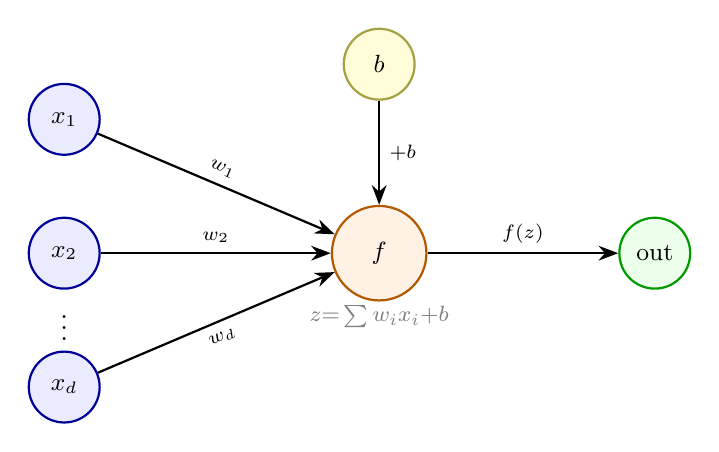
\begin{tikzpicture}[
    node distance=1.8cm,
    input/.style={circle, draw=blue!60!black, fill=blue!8, thick, minimum size=0.9cm, font=\small},
    neuron/.style={circle, draw=orange!70!black, fill=orange!10, thick, minimum size=1.2cm, font=\small\bfseries},
    output/.style={circle, draw=green!60!black, fill=green!8, thick, minimum size=0.9cm, font=\small},
    arr/.style={-{Stealth[length=2.5mm]}, thick}
]
  \node[input] (x1) at (0,  2.5) {$x_1$};
  \node[input] (x2) at (0,  0.8) {$x_2$};
  \node[input] (xd) at (0, -0.9) {$x_d$};
  \node at (0, -0.05) {\vdots};

  \node[neuron] (n) at (4.0, 0.8) {$f$};
  \node[input, fill=yellow!15, draw=yellow!60!black] (b) at (4.0, 3.2) {$b$};
  \node[output] (y) at (7.5, 0.8) {out};

  \draw[arr] (x1) -- node[above, sloped, font=\scriptsize]{$w_1$} (n);
  \draw[arr] (x2) -- node[above, font=\scriptsize]{$w_2$} (n);
  \draw[arr] (xd) -- node[below, sloped, font=\scriptsize]{$w_d$} (n);
  \draw[arr] (b)  -- node[right, font=\scriptsize]{$+b$} (n);
  \draw[arr] (n)  -- node[above, font=\scriptsize]{$f(z)$} (y);

  \node[font=\footnotesize, gray] at (4.0, 0.0) {$z{=}\sum w_i x_i{+}b$};
\end{tikzpicture}
\end{center}

\begin{examplebox}{A Single Neuron, Step by Step}
Let us compute the output of a single neuron with two inputs by hand.

\textbf{Given values:}
\begin{itemize}
    \item Inputs: $x_1 = 0.5$, $x_2 = 0.3$
    \item Weights: $w_1 = 0.8$, $w_2 = -0.4$
    \item Bias: $b = 0.1$
\end{itemize}

\textbf{Step 1 --- Compute the weighted sum (pre-activation):}
\begin{align*}
    z &= w_1 \cdot x_1 + w_2 \cdot x_2 + b \\
      &= 0.8 \times 0.5 + (-0.4) \times 0.3 + 0.1 \\
      &= 0.40 - 0.12 + 0.10 \\
      &= 0.38
\end{align*}

\textbf{Step 2a --- Apply ReLU activation:}
\[
    f_{\text{ReLU}}(z) = \max(0,\, z) = \max(0,\, 0.38) = \mathbf{0.38}
\]

\textbf{Step 2b --- Apply sigmoid activation instead:}
\[
    f_{\text{sigmoid}}(z) = \frac{1}{1 + e^{-z}} = \frac{1}{1 + e^{-0.38}}
\]
We need $e^{-0.38}$. Since $e^{0.38} \approx 1.462$, we have $e^{-0.38} \approx 0.684$. Therefore:
\[
    f_{\text{sigmoid}}(0.38) = \frac{1}{1 + 0.684} = \frac{1}{1.684} \approx \mathbf{0.594}
\]

\textbf{Interpretation:} With ReLU the neuron simply passes through the positive pre-activation $0.38$. With sigmoid the neuron maps $0.38$ to a value in $(0,1)$, which can be read as a ``soft probability'' of roughly $59.4\%$.
\end{examplebox}

\begin{keyinsight}{Why the Bias Matters}
Without the bias $b$, every neuron's output would be zero when all inputs are zero. The bias is like a ``default level of activity'' that shifts the neuron's sensitivity threshold. In practice, removing biases makes it significantly harder for the network to learn, because the function $f(\sum w_i x_i)$ is constrained to pass through the origin.
\end{keyinsight}

% ============================================================
\section{Activation Functions}
\label{sec:activations}

Without a non-linear activation function, a stack of neurons is mathematically equivalent to a single linear transformation --- no matter how many layers you add. Activation functions are the source of a neural network's expressive power.

\subsection{ReLU: The Most Widely Used Activation}

\begin{mathbox}{ReLU --- Rectified Linear Unit}
\begin{equation}
    f_{\text{ReLU}}(x) = \max(0,\; x) =
    \begin{cases}
        x & \text{if } x > 0 \\
        0 & \text{if } x \le 0
    \end{cases}
\end{equation}
\textbf{Derivative:} $f'_{\text{ReLU}}(x) = \mathbf{1}[x > 0]$ (1 for positive inputs, 0 for non-positive inputs).
\end{mathbox}

ReLU ``kills'' all negative pre-activations by setting them to zero. This sounds harsh but has a crucial benefit: because $f'(x) = 1$ for all $x > 0$, gradients do not shrink as they pass through active neurons. This solved the \emph{vanishing gradient problem} that crippled deep networks with sigmoid and tanh activations.

\begin{examplebox}{ReLU Input-Output Table}
\begin{center}
\renewcommand{\arraystretch}{1.3}
\begin{tabular}{rrl}
\toprule
Input $x$ & $\max(0, x)$ & Note \\
\midrule
$-3.0$ & $0.0$ & negative input, killed \\
$-0.5$ & $0.0$ & negative input, killed \\
$0.0$  & $0.0$ & boundary \\
$0.5$  & $0.5$ & positive, passed through unchanged \\
$1.8$  & $1.8$ & positive, passed through unchanged \\
$5.2$  & $5.2$ & positive, passed through unchanged \\
\bottomrule
\end{tabular}
\end{center}
Notice that ReLU is linear on the positive half --- it does not compress large positive values. This is a deliberate design choice that helps gradients flow during training.
\end{examplebox}

\subsection{Sigmoid: Squashing to Probabilities}

\begin{mathbox}{Sigmoid Function}
\begin{equation}
    f_{\text{sigmoid}}(x) = \frac{1}{1 + e^{-x}}
\end{equation}
\textbf{Range:} $(0, 1)$. As $x \to +\infty$, $f \to 1$. As $x \to -\infty$, $f \to 0$.\\
\textbf{Derivative:} $f'(x) = f(x)\bigl(1 - f(x)\bigr)$.
\end{mathbox}

Sigmoid is useful at the \emph{output} layer of binary classifiers because it maps any real number to a value interpretable as a probability. However, its derivative is at most $0.25$, which causes gradients to shrink rapidly in deep networks --- this is why it is rarely used in hidden layers today.

\begin{examplebox}{Sigmoid at a Few Key Points}
\begin{center}
\renewcommand{\arraystretch}{1.3}
\begin{tabular}{rl}
\toprule
$x$ & $1/(1+e^{-x})$ \\
\midrule
$-4$ & $\approx 0.018$ \\
$-2$ & $\approx 0.119$ \\
$0$  & $= 0.500$ \\
$2$  & $\approx 0.881$ \\
$4$  & $\approx 0.982$ \\
\bottomrule
\end{tabular}
\end{center}
Sigmoid is symmetric around $x=0$ where its output is exactly $0.5$. Very large or very small inputs produce outputs near 1 or 0 respectively --- the function \emph{saturates}.
\end{examplebox}

\subsection{Softmax: Turning Scores into a Probability Distribution}

When we have $k$ mutually exclusive classes (for us: $k = N$ nodes, one is the source), we need the output to form a valid probability distribution: all values in $[0,1]$ and summing to exactly 1. Softmax achieves this.

\begin{mathbox}{Softmax Function}
Given a vector of raw scores (logits) $\mathbf{z} = [z_1, z_2, \ldots, z_k]$, the softmax function converts them into probabilities:
\begin{equation}
    \text{softmax}(z_i) = \frac{e^{z_i}}{\displaystyle\sum_{j=1}^{k} e^{z_j}}
    \quad \text{for } i = 1, 2, \ldots, k
\end{equation}
\textbf{Properties:} each output is in $(0,1)$; all outputs sum to exactly 1; the largest $z_i$ receives the highest probability; the ordering is preserved.
\end{mathbox}

\begin{examplebox}{Softmax on Three Scores, Worked Fully}
Suppose our network produces logits $\mathbf{z} = [1.0,\; 2.0,\; 0.5]$ for three candidate sources.

\textbf{Step 1 --- Compute exponentials:}
\begin{align*}
    e^{z_1} = e^{1.0} &\approx 2.718 \\
    e^{z_2} = e^{2.0} &\approx 7.389 \\
    e^{z_3} = e^{0.5} &\approx 1.649
\end{align*}

\textbf{Step 2 --- Sum:}
\[
    S = 2.718 + 7.389 + 1.649 = 11.756
\]

\textbf{Step 3 --- Divide each by the sum:}
\begin{align*}
    p_1 &= 2.718 / 11.756 \approx 0.231 \\
    p_2 &= 7.389 / 11.756 \approx 0.628 \\
    p_3 &= 1.649 / 11.756 \approx 0.140
\end{align*}

\textbf{Verification:} $0.231 + 0.628 + 0.140 = 0.999 \approx 1$ (rounding error only). \\
\textbf{Interpretation:} The network assigns 62.8\% probability to node 2 being the source, 23.1\% to node 1, and 14.0\% to node 3.
\end{examplebox}

\subsection{Log-Softmax: Numerical Stability in Practice}

Computing $\log(\text{softmax}(\mathbf{z}))$ naively can cause numerical overflow when any $z_i$ is large (e.g.\ $e^{1000} = \infty$ in floating point). The \textbf{log-softmax} function avoids this by exploiting the identity $\log(a/b) = \log a - \log b$ and subtracting the maximum logit before exponentiation.

\begin{mathbox}{Log-Softmax (Numerically Stable Form)}
\begin{equation}
    \log\text{-softmax}(z_i) = z_i - \log\!\left(\sum_{j=1}^{k} e^{z_j}\right)
\end{equation}
In practice, the \textbf{log-sum-exp trick} subtracts $\max_j z_j$ from all logits before exponentiating, which keeps all values in a safe numerical range without changing the result.

This is exactly what \texttt{F.log\_softmax(x, dim=1)} computes in PyTorch.
\end{mathbox}

\begin{examplebox}{Log-Softmax on the Same Three Scores}
Continuing from $\mathbf{z} = [1.0, 2.0, 0.5]$ and $S = 11.756$:
\[
    \log S = \log(11.756) \approx 2.464
\]
\begin{align*}
    \log\text{-softmax}(z_1) &= 1.0 - 2.464 = -1.464 \\
    \log\text{-softmax}(z_2) &= 2.0 - 2.464 = -0.464 \\
    \log\text{-softmax}(z_3) &= 0.5 - 2.464 = -1.964
\end{align*}
\textbf{Verification:} $e^{-1.464} \approx 0.231$, $e^{-0.464} \approx 0.629$, $e^{-1.964} \approx 0.140$ --- these match the softmax probabilities above exactly.

\textbf{Log-probabilities are always $\le 0$}, which makes sense: $\log(p) \le 0$ for $p \in (0,1)$.
\end{examplebox}

\subsection{PReLU: A Learnable Activation}

\begin{mathbox}{PReLU --- Parametric Rectified Linear Unit}
\begin{equation}
    f_{\text{PReLU}}(x;\, \alpha) = \max(\alpha x,\; x) =
    \begin{cases}
        x    & \text{if } x \ge 0 \\
        \alpha x & \text{if } x < 0
    \end{cases}
\end{equation}
Here $\alpha$ is a \textbf{learnable scalar parameter} (one per channel, initialized at $0.25$). The gradient with respect to $\alpha$ is $\frac{\partial}{\partial \alpha} f = x \cdot \mathbf{1}[x < 0]$, so $\alpha$ is updated by standard backpropagation.
\end{mathbox}

PReLU generalizes ReLU: if $\alpha = 0$ it reduces to ReLU; if $\alpha = 0.01$ it becomes Leaky ReLU. The key advantage is that the network can \emph{learn} how much signal to let through on the negative side, rather than fixing it to zero. Every convolution block in \texttt{gnn/static\_gnn.py} uses \texttt{torch.nn.PReLU()} precisely for this reason.

\begin{keyinsight}{Choosing an Activation Function}
\begin{itemize}
    \item Use \textbf{ReLU} or \textbf{PReLU} in hidden layers. They avoid vanishing gradients and are computationally cheap.
    \item Use \textbf{sigmoid} in the output layer only when you need a binary probability.
    \item Use \textbf{softmax} (or log-softmax) in the output layer when you need a probability distribution over $k \ge 2$ classes.
    \item \textbf{Never use sigmoid or tanh in hidden layers} of deep networks unless you have a specific reason --- their saturating behavior makes training slow or impossible.
\end{itemize}
\end{keyinsight}

% ============================================================
\section{Layers and the Forward Pass}
\label{sec:forward_pass}

\subsection{What is a Layer?}

A \textbf{layer} is a set of neurons that all receive the same input vector and produce an output vector in parallel. If a layer has $m$ neurons and each receives a $d$-dimensional input, the layer applies $m$ different neurons simultaneously and stacks their outputs into a single vector of length $m$.

\begin{conceptbox}{Layer as a Matrix-Vector Operation}
A single layer with $m$ neurons and $d$-dimensional input can be written compactly as:
\begin{equation}
    \mathbf{h} = f\!\left(\mathbf{W}\mathbf{x} + \mathbf{b}\right)
\end{equation}
where:
\begin{itemize}
    \item $\mathbf{x} \in \mathbb{R}^d$ --- input vector ($d$ values from the previous layer or raw features)
    \item $\mathbf{W} \in \mathbb{R}^{m \times d}$ --- weight matrix (row $i$ contains the weights for neuron $i$)
    \item $\mathbf{b} \in \mathbb{R}^m$ --- bias vector (one bias per neuron)
    \item $f$ --- activation function applied \textbf{element-wise} to each entry of $\mathbf{Wx}+\mathbf{b}$
    \item $\mathbf{h} \in \mathbb{R}^m$ --- output vector (one value per neuron)
\end{itemize}
The learnable parameters of this layer are $\{\mathbf{W},\, \mathbf{b}\}$, totalling $m \cdot d + m = m(d+1)$ numbers.
\end{conceptbox}

\subsection{A Two-Layer Network}

Let us define a small but concrete two-layer network and trace a data point through it.

\begin{conceptbox}{Architecture: Input $\to$ Hidden $\to$ Output}
\begin{itemize}
    \item Input layer: $\mathbf{x} \in \mathbb{R}^2$ (2 raw features)
    \item Hidden layer: $\mathbf{h} \in \mathbb{R}^3$ (3 neurons, ReLU activation)
    \item Output layer: $y \in \mathbb{R}^1$ (1 neuron, no activation in this example)
\end{itemize}
\textbf{Equations:}
\begin{align}
    \mathbf{h} &= \text{ReLU}\!\left(\mathbf{W}^{(1)}\mathbf{x} + \mathbf{b}^{(1)}\right) \label{eq:layer1} \\
    y           &= \mathbf{W}^{(2)}\mathbf{h} + b^{(2)} \label{eq:layer2}
\end{align}
where $\mathbf{W}^{(1)} \in \mathbb{R}^{3 \times 2}$, $\mathbf{b}^{(1)} \in \mathbb{R}^{3}$, $\mathbf{W}^{(2)} \in \mathbb{R}^{1 \times 3}$, $b^{(2)} \in \mathbb{R}$.
\end{conceptbox}

\begin{examplebox}{Forward Pass Through a Two-Layer Network (Fully Numerical)}
\textbf{Weights (given, as if randomly initialized):}
\[
    \mathbf{W}^{(1)} = \begin{bmatrix} 0.1 & 0.2 \\ 0.3 & -0.1 \\ 0.5 & 0.4 \end{bmatrix}, \quad
    \mathbf{b}^{(1)} = \begin{bmatrix} 0 \\ 0 \\ 0 \end{bmatrix}, \quad
    \mathbf{W}^{(2)} = \begin{bmatrix} 1.0 & -0.5 & 0.3 \end{bmatrix}, \quad
    b^{(2)} = 0
\]

\textbf{Input:} $\mathbf{x} = [1.0,\; 2.0]^\top$

\textbf{Step 1 --- Pre-activation of hidden layer:}
\[
    \mathbf{z}^{(1)} = \mathbf{W}^{(1)}\mathbf{x} =
    \begin{bmatrix} 0.1 \cdot 1.0 + 0.2 \cdot 2.0 \\ 0.3 \cdot 1.0 + (-0.1) \cdot 2.0 \\ 0.5 \cdot 1.0 + 0.4 \cdot 2.0 \end{bmatrix}
    = \begin{bmatrix} 0.1 + 0.4 \\ 0.3 - 0.2 \\ 0.5 + 0.8 \end{bmatrix}
    = \begin{bmatrix} 0.5 \\ 0.1 \\ 1.3 \end{bmatrix}
\]

\textbf{Step 2 --- Apply ReLU element-wise:}
\[
    \mathbf{h} = \text{ReLU}\!\left(\begin{bmatrix}0.5\\0.1\\1.3\end{bmatrix}\right)
    = \begin{bmatrix}\max(0,0.5)\\\max(0,0.1)\\\max(0,1.3)\end{bmatrix}
    = \begin{bmatrix}0.5\\0.1\\1.3\end{bmatrix}
\]
All three pre-activations are positive, so ReLU leaves them unchanged.

\textbf{Step 3 --- Output layer:}
\[
    y = \mathbf{W}^{(2)}\mathbf{h} = 1.0 \cdot 0.5 + (-0.5) \cdot 0.1 + 0.3 \cdot 1.3
      = 0.5 - 0.05 + 0.39 = \mathbf{0.84}
\]
The raw score for this input is $0.84$. In a classification setting, this would next be passed through softmax along with the scores for all other classes.
\end{examplebox}

\begin{center}
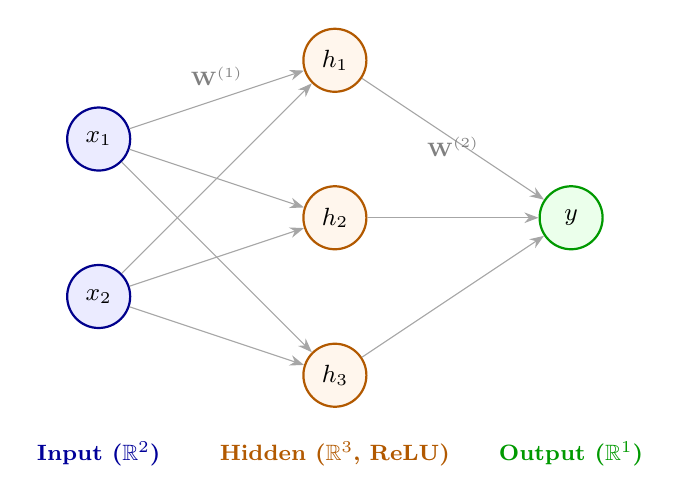
\begin{tikzpicture}[
    every node/.style={font=\small},
    inp/.style={circle, draw=blue!55!black, fill=blue!8, thick, minimum size=0.8cm},
    hid/.style={circle, draw=orange!70!black, fill=orange!7, thick, minimum size=0.8cm},
    outn/.style={circle, draw=green!60!black, fill=green!8, thick, minimum size=0.8cm},
    arr/.style={-{Stealth[length=1.8mm]}, gray!70, thin}
]
  \node[inp] (i1) at (0,  1.0) {$x_1$};
  \node[inp] (i2) at (0, -1.0) {$x_2$};

  \node[hid] (h1) at (3.0,  2.0) {$h_1$};
  \node[hid] (h2) at (3.0,  0.0) {$h_2$};
  \node[hid] (h3) at (3.0, -2.0) {$h_3$};

  \node[outn] (y)  at (6.0,  0.0) {$y$};

  \foreach \s in {1,2}{
    \foreach \t in {1,2,3}{
      \draw[arr] (i\s) -- (h\t);
    }
  }
  \foreach \t in {1,2,3}{
    \draw[arr] (h\t) -- (y);
  }

  \node[blue!60!black,  font=\footnotesize\bfseries] at (0,  -3.0) {Input ($\mathbb{R}^2$)};
  \node[orange!70!black, font=\footnotesize\bfseries] at (3.0, -3.0) {Hidden ($\mathbb{R}^3$, ReLU)};
  \node[green!60!black,  font=\footnotesize\bfseries] at (6.0, -3.0) {Output ($\mathbb{R}^1$)};

  \node[gray, font=\scriptsize] at (1.5,  1.8) {$\mathbf{W}^{(1)}$};
  \node[gray, font=\scriptsize] at (4.5,  0.9) {$\mathbf{W}^{(2)}$};
\end{tikzpicture}
\end{center}

\subsection{Deep Networks: Stacking Many Layers}

A \textbf{deep network} (or deep neural network) stacks multiple hidden layers. Each layer transforms the representation produced by the previous layer.

\begin{mathbox}{$L$-Layer MLP Forward Pass}
An $L$-layer network computes:
\begin{align}
    \mathbf{h}^{(0)} &= \mathbf{x} \quad \text{(input)} \\
    \mathbf{z}^{(l)} &= \mathbf{W}^{(l)}\mathbf{h}^{(l-1)} + \mathbf{b}^{(l)} \quad \text{for } l = 1, \ldots, L \quad \text{(pre-activation)} \\
    \mathbf{h}^{(l)} &= f\!\left(\mathbf{z}^{(l)}\right) \quad \text{for } l = 1, \ldots, L-1 \quad \text{(hidden activations)} \\
    \hat{\mathbf{y}}  &= g\!\left(\mathbf{z}^{(L)}\right) \quad \text{(output activation, e.g.\ log-softmax)}
\end{align}
The total parameter count is $\sum_{l=1}^{L} \bigl( d_{l-1} \cdot d_l + d_l \bigr)$ where $d_l$ is the width of layer $l$ and $d_0 = d$ is the input dimension.
\end{mathbox}

% ============================================================
\section{Loss Functions}
\label{sec:loss_functions}

A \textbf{loss function} $\mathcal{L}(\hat{\mathbf{y}},\, \mathbf{y})$ measures how wrong the network's prediction $\hat{\mathbf{y}}$ is compared to the true answer $\mathbf{y}$. Training \emph{minimizes} this loss over the training dataset.

\begin{analogybox}{The Loss as a Navigation Error}
Imagine you are navigating with GPS and the GPS tells you that you are 3 km off course. That ``3 km'' is the loss. You want to reduce it to zero by adjusting your heading (your weights). The direction to turn is given by the gradient --- more on that in the next section.
\end{analogybox}

\subsection{Cross-Entropy Loss for Classification}

When the task is classification --- predicting which of $N$ classes is correct --- we use \textbf{cross-entropy loss}. In our case, $N$ is the number of nodes, and the correct class is the true source node.

\begin{mathbox}{Cross-Entropy Loss}
Let $\hat{\mathbf{y}} \in (0,1)^N$ be the network's predicted probability distribution over $N$ classes, and let $\mathbf{y}$ be the true label (a one-hot vector with a single 1 at position $c^*$, the correct class). The cross-entropy loss is:
\begin{equation}
    \mathcal{L}_{\text{CE}} = -\sum_{c=1}^{N} y_c \log \hat{y}_c
\end{equation}
Since $y_c = 0$ for all $c \ne c^*$ and $y_{c^*} = 1$, all but one term vanish:
\begin{equation}
    \mathcal{L}_{\text{CE}} = -\log \hat{y}_{c^*}
\end{equation}
The loss is simply the negative log-probability assigned to the correct class.

\textbf{Intuition:} If the model is very confident and correct ($\hat{y}_{c^*} \approx 1$), then $-\log(1) = 0$ --- zero loss. If the model is wrong and confident ($\hat{y}_{c^*} \approx 0$), then $-\log(0) = +\infty$ --- infinite loss.
\end{mathbox}

\begin{examplebox}{Cross-Entropy: Three Classes}
Suppose we have 3 candidate nodes. The network predicts $\hat{\mathbf{y}} = [0.1,\; 0.7,\; 0.2]$ and the true source is \textbf{node 2} (index 2, the middle one, with $\hat{y}_2 = 0.7$).

\[
    \mathcal{L}_{\text{CE}} = -\log \hat{y}_{c^*} = -\log(0.7) \approx \mathbf{0.357}
\]

Now imagine the network was instead very uncertain: $\hat{\mathbf{y}} = [0.33,\; 0.34,\; 0.33]$:
\[
    \mathcal{L}_{\text{CE}} = -\log(0.34) \approx \mathbf{1.079}
\]

And if the model was wrong and confident: $\hat{\mathbf{y}} = [0.9,\; 0.05,\; 0.05]$ (predicted node 1 instead of node 2):
\[
    \mathcal{L}_{\text{CE}} = -\log(0.05) \approx \mathbf{2.996}
\]

The loss correctly penalizes confident wrong answers most heavily.
\end{examplebox}

\begin{examplebox}{Source Detection as Classification}
In our source detection task, the network observes an SIR snapshot (which nodes are Susceptible, Infected, or Recovered) on a graph with $N$ nodes. It must output a probability for each of the $N$ nodes being the source.

This is an $N$-class classification problem. For a network with $N = 500$ nodes:
\begin{itemize}
    \item The output layer has 500 neurons.
    \item Log-softmax produces 500 log-probabilities.
    \item The true source has label 1 (gets the ``correct class'' slot).
    \item All other 499 nodes have label 0.
    \item The NLL loss picks out just the log-probability assigned to the true source.
\end{itemize}

A uniform (random-guessing) model would assign $\hat{y}_{c^*} = 1/500 = 0.002$, giving a loss of $-\log(0.002) \approx 6.2$. A well-trained model should drive this loss down significantly.
\end{examplebox}

\subsection{NLL Loss: What the Code Uses}

When the model outputs \emph{log-probabilities} (as our \texttt{StaticGNN} does via \texttt{F.log\_softmax}), the appropriate loss is the \textbf{Negative Log-Likelihood (NLL)} loss:

\begin{mathbox}{NLL Loss}
Let $\hat{q}_{c^*} = \log \hat{y}_{c^*}$ be the log-probability assigned to the correct class. Then:
\begin{equation}
    \mathcal{L}_{\text{NLL}} = -\hat{q}_{c^*}
\end{equation}
This is identical to cross-entropy when the model uses log-softmax. The combination \texttt{F.log\_softmax + nn.NLLLoss} is numerically more stable than \texttt{F.softmax + cross\_entropy} because it avoids computing $\exp$ and then $\log$ in sequence.
\end{mathbox}

% ============================================================
\section{Backpropagation --- The Chain Rule in Action}
\label{sec:backprop}

We now know how to compute a forward pass (get a prediction) and a loss (measure the error). What we need next is a method to compute the gradient of the loss with respect to every weight in the network. This is \textbf{backpropagation}.

\begin{analogybox}{Backpropagation as Blame Attribution}
Imagine a factory assembly line. A defective product rolls off the end. Who is to blame? The quality inspector at the end traces the defect backward: first to the packaging station, then to the assembly station, then to the raw materials. Each station gets assigned a ``blame score'' proportional to how much its error contributed to the final defect.

Backpropagation does exactly this for a neural network. The loss at the end is the ``defect.'' Backpropagation traces it backward through all the layers, computing how much each weight contributed to the loss.
\end{analogybox}

\subsection{The Chain Rule: Derivatives Through Compositions}

If you have a function composed of two operations --- $L = g(f(w))$ --- then the chain rule gives:
\begin{equation}
    \frac{dL}{dw} = \frac{dL}{df} \cdot \frac{df}{dw}
\end{equation}
In words: ``how much does $L$ change if I wiggle $w$?'' equals ``how much does $L$ change if I wiggle $f$'' times ``how much does $f$ change if I wiggle $w$.''

\begin{conceptbox}{The Chain Rule in a Neural Network}
For a weight $w$ in layer $l$ of a network, the gradient flows backward through the chain:
\[
    \frac{\partial \mathcal{L}}{\partial w} =
    \underbrace{\frac{\partial \mathcal{L}}{\partial z^{(L)}}}_{\text{loss grad at output}}
    \cdot
    \underbrace{\frac{\partial z^{(L)}}{\partial \cdots}}_{\text{chain through upper layers}}
    \cdot
    \underbrace{\frac{\partial z^{(l)}}{\partial w}}_{\text{local contribution}}
\]
Each term in the chain is a local derivative that can be computed analytically. The \emph{product} of all these local derivatives gives the gradient of the global loss with respect to any specific weight.
\end{conceptbox}

\begin{examplebox}{Backpropagation Through a Single Neuron}
We will trace the gradient from loss to weight for the single neuron computed earlier.

\textbf{Setup:}
\begin{itemize}
    \item Inputs: $x_1 = 0.5$, $x_2 = 0.3$; Weights: $w_1 = 0.8$, $w_2 = -0.4$; Bias: $b = 0.1$
    \item Pre-activation: $z = 0.38$; Activation: sigmoid; output: $\hat{y} = 0.594$
    \item True label: $y = 1.0$; Loss: squared loss $\mathcal{L} = \frac{1}{2}(\hat{y} - y)^2$
\end{itemize}

\textbf{Forward values (already computed):}
\[
    z = 0.38, \quad \hat{y} = \sigma(0.38) \approx 0.594
\]

\textbf{Step 1 --- Gradient of loss w.r.t.\ output:}
\[
    \frac{\partial \mathcal{L}}{\partial \hat{y}} = \hat{y} - y = 0.594 - 1.0 = -0.406
\]
(The loss decreases as $\hat{y}$ increases, so the gradient is negative.)

\textbf{Step 2 --- Gradient through the sigmoid} (chain rule):
\[
    \frac{\partial \hat{y}}{\partial z} = \sigma(z)(1 - \sigma(z)) = 0.594 \times (1 - 0.594) = 0.594 \times 0.406 \approx 0.241
\]
\[
    \frac{\partial \mathcal{L}}{\partial z} = \frac{\partial \mathcal{L}}{\partial \hat{y}} \cdot \frac{\partial \hat{y}}{\partial z} = (-0.406) \times 0.241 \approx -0.098
\]

\textbf{Step 3 --- Gradient of $z$ w.r.t.\ each weight:}
\[
    \frac{\partial z}{\partial w_1} = x_1 = 0.5, \quad
    \frac{\partial z}{\partial w_2} = x_2 = 0.3, \quad
    \frac{\partial z}{\partial b}  = 1
\]

\textbf{Step 4 --- Final gradients via the chain rule:}
\begin{align*}
    \frac{\partial \mathcal{L}}{\partial w_1} &= \frac{\partial \mathcal{L}}{\partial z} \cdot \frac{\partial z}{\partial w_1} = (-0.098) \times 0.5 = -0.049 \\
    \frac{\partial \mathcal{L}}{\partial w_2} &= \frac{\partial \mathcal{L}}{\partial z} \cdot \frac{\partial z}{\partial w_2} = (-0.098) \times 0.3 = -0.029 \\
    \frac{\partial \mathcal{L}}{\partial b}   &= \frac{\partial \mathcal{L}}{\partial z} \cdot 1 = -0.098
\end{align*}

\textbf{Interpretation:} Each gradient tells us ``if I increase this weight by a tiny amount $\epsilon$, the loss changes by gradient $\times \epsilon$.'' The gradients are negative, so increasing $w_1$ and $w_2$ would \emph{decrease} the loss. Gradient descent will do exactly that.
\end{examplebox}

\subsection{Gradients as Infinitesimal Sensitivity}

\begin{keyinsight}{What a Gradient Really Means}
The gradient $\frac{\partial \mathcal{L}}{\partial w}$ answers the question: ``If I increase $w$ by a very small amount $\epsilon$, how much does the loss change?''

\[
    \mathcal{L}(w + \epsilon) \approx \mathcal{L}(w) + \epsilon \cdot \frac{\partial \mathcal{L}}{\partial w}
\]

A gradient of $-0.049$ for $w_1$ means: increase $w_1$ by $0.001$ and the loss decreases by $0.049 \times 0.001 = 0.000049$. This is tiny, but gradient descent applies this update thousands of times, cumulatively moving the weights to a region of low loss.
\end{keyinsight}

% ============================================================
\section{Gradient Descent and Optimizers}
\label{sec:optimizers}

Now that we have gradients, we use them to update the weights. The goal is to move the weights in the direction that \emph{decreases} the loss.

\subsection{Vanilla Gradient Descent}

\begin{mathbox}{Gradient Descent Update Rule}
For each learnable parameter $w$, the update is:
\begin{equation}
    w \leftarrow w - \eta \cdot \frac{\partial \mathcal{L}}{\partial w}
\end{equation}
where $\eta > 0$ is the \textbf{learning rate} (also written $\alpha$ or $\text{lr}$ in code).
\end{mathbox}

The minus sign is essential: we subtract the gradient because we want to go \emph{downhill}. If the gradient is positive (loss increases as $w$ increases), we decrease $w$. If the gradient is negative, we increase $w$.

\begin{analogybox}{Gradient Descent as Hiking Downhill Blindfolded}
Imagine you are blindfolded on a hilly landscape and your goal is to reach the lowest valley (minimum loss). You cannot see the whole terrain. The only thing you can do is feel the slope under your feet (the gradient) and take one step in the downhill direction.

\begin{itemize}
    \item \textbf{Learning rate too large:} your steps are so big that you overshoot the valley and land on the other side, maybe even on a higher hill. The loss oscillates or diverges.
    \item \textbf{Learning rate too small:} your steps are so tiny that it takes millions of steps to get anywhere. Training is painfully slow.
    \item \textbf{Learning rate just right:} you smoothly descend to the valley in a reasonable number of steps.
\end{itemize}
\end{analogybox}

\begin{examplebox}{One Gradient Descent Step on Our Single Neuron}
From the previous example, the gradients were:
\[
    \frac{\partial \mathcal{L}}{\partial w_1} = -0.049, \quad
    \frac{\partial \mathcal{L}}{\partial w_2} = -0.029, \quad
    \frac{\partial \mathcal{L}}{\partial b} = -0.098
\]
With learning rate $\eta = 0.1$, the new weights are:
\begin{align*}
    w_1 &\leftarrow 0.8 - 0.1 \times (-0.049) = 0.8 + 0.0049 = 0.8049 \\
    w_2 &\leftarrow -0.4 - 0.1 \times (-0.029) = -0.4 + 0.0029 = -0.3971 \\
    b   &\leftarrow 0.1 - 0.1 \times (-0.098) = 0.1 + 0.0098 = 0.1098
\end{align*}
After this update, the neuron's pre-activation for the same input would be:
\[
    z_{\text{new}} = 0.8049 \times 0.5 + (-0.3971) \times 0.3 + 0.1098
    = 0.4025 - 0.1191 + 0.1098 = 0.3932
\]
The output would be $\sigma(0.3932) \approx 0.597$, slightly closer to the target $y = 1.0$. Repeating this process thousands of times converges to a good solution.
\end{examplebox}

\subsection{Stochastic and Mini-Batch Gradient Descent}

In practice, computing the gradient on the entire training dataset before each update is too expensive. Instead:

\begin{itemize}
    \item \textbf{Stochastic gradient descent (SGD):} compute gradient on one random training example per step. Fast but noisy.
    \item \textbf{Mini-batch SGD:} compute gradient on a small random batch of $B$ examples (typically $B \in \{16, 32, 64, 128\}$). Best of both worlds: less noisy than SGD but much faster than full-batch.
\end{itemize}

\subsection{The Adam Optimizer}

Plain gradient descent uses the same learning rate $\eta$ for every parameter. In a neural network, some weights receive large gradients and others receive tiny ones. A single fixed $\eta$ is a poor fit for such heterogeneous dynamics.

\textbf{Adam} (Adaptive Moment Estimation, Kingma \& Ba, 2015) maintains a separate, adaptive learning rate for each parameter by tracking the exponentially weighted average of its recent gradients (first moment) and their squares (second moment).

\begin{mathbox}{Adam Update Equations}
At time step $t$, given gradient $g_t = \nabla_w \mathcal{L}_t$:

\begin{align}
    m_t &= \beta_1 m_{t-1} + (1 - \beta_1) g_t \quad & \text{(first moment: moving average of gradients)} \\
    v_t &= \beta_2 v_{t-1} + (1 - \beta_2) g_t^2 \quad & \text{(second moment: moving average of squared gradients)} \\
    \hat{m}_t &= \frac{m_t}{1 - \beta_1^t} \quad & \text{(bias-corrected first moment)} \\
    \hat{v}_t &= \frac{v_t}{1 - \beta_2^t} \quad & \text{(bias-corrected second moment)} \\
    w_t &= w_{t-1} - \eta \cdot \frac{\hat{m}_t}{\sqrt{\hat{v}_t} + \varepsilon} \quad & \text{(parameter update)}
\end{align}

\textbf{Default hyperparameters:} $\beta_1 = 0.9$, $\beta_2 = 0.999$, $\varepsilon = 10^{-8}$.
\end{mathbox}

Let us unpack each symbol:
\begin{itemize}
    \item $m_t$: the \emph{momentum} term --- a running average of past gradients. If recent gradients consistently point in the same direction, $m_t$ accumulates that direction and the update accelerates (like a ball rolling downhill gathering momentum).
    \item $v_t$: the \emph{second moment} --- a running average of past \emph{squared} gradients. Parameters that have been receiving large gradients will have a large $v_t$.
    \item $\hat{m}_t / (\sqrt{\hat{v}_t} + \varepsilon)$: the effective step size. Parameters with large recent gradients get a smaller effective step (the large $\sqrt{\hat{v}_t}$ in the denominator), preventing them from overshooting.
    \item $\varepsilon = 10^{-8}$: a small constant that prevents division by zero.
    \item The bias correction terms $(1 - \beta_1^t)$ and $(1 - \beta_2^t)$ account for the fact that $m_0 = v_0 = 0$ --- early estimates are biased toward zero and need to be corrected.
\end{itemize}

\begin{examplebox}{One Adam Step (Simplified, Single Parameter)}
Let $w = 0.8$, $\eta = 0.001$, $\beta_1 = 0.9$, $\beta_2 = 0.999$, $\varepsilon = 10^{-8}$. Say this is step $t=1$ and the gradient is $g_1 = -0.049$ (from our earlier example). Starting from $m_0 = 0$, $v_0 = 0$:
\begin{align*}
    m_1 &= 0.9 \times 0 + 0.1 \times (-0.049) = -0.0049 \\
    v_1 &= 0.999 \times 0 + 0.001 \times (-0.049)^2 = 0.001 \times 0.002401 = 2.401 \times 10^{-6} \\
    \hat{m}_1 &= -0.0049 / (1 - 0.9^1) = -0.0049 / 0.1 = -0.049 \\
    \hat{v}_1 &= 2.401 \times 10^{-6} / (1 - 0.999^1) = 2.401 \times 10^{-6} / 0.001 = 2.401 \times 10^{-3} \\
    w_1 &= 0.8 - 0.001 \times \frac{-0.049}{\sqrt{2.401 \times 10^{-3}} + 10^{-8}}
          = 0.8 - 0.001 \times \frac{-0.049}{0.04900}
          = 0.8 + 0.001 = \mathbf{0.801}
\end{align*}
At step 1, the bias correction makes $\hat{m}_1 = g_1$ and the adaptive learning rate effectively normalizes the step to $\pm 0.001$, regardless of gradient magnitude. This ``warm start'' normalization is what makes Adam reliable without careful learning rate tuning.
\end{examplebox}

% ============================================================
\section{Batch Normalization}
\label{sec:batchnorm}

\subsection{The Problem: Shifting Input Distributions}

During training, every time we update the weights in layer $l$, the \emph{distribution of inputs} to layer $l+1$ shifts. This is called \textbf{internal covariate shift}. It means each layer must constantly re-adapt to a moving target, which slows training.

\begin{analogybox}{Batch Normalization as Zeroing Out Jet Lag}
Imagine you are training for a marathon by running in a different city every day --- sometimes at sea level, sometimes at altitude, sometimes in heat. Your body wastes energy adapting to the new environment rather than building fitness. Batch normalization is like training in a perfectly consistent, standardized environment: the same altitude, temperature, and humidity every day, so your body can focus on becoming a better runner.
\end{analogybox}

\subsection{The BatchNorm Formula}

\begin{mathbox}{Batch Normalization}
Given a mini-batch $\mathcal{B} = \{x_1, x_2, \ldots, x_M\}$ of pre-activations (a single feature dimension across $M$ examples):

\begin{align}
    \mu_\mathcal{B} &= \frac{1}{M} \sum_{i=1}^{M} x_i \quad & \text{(mini-batch mean)} \\
    \sigma^2_\mathcal{B} &= \frac{1}{M} \sum_{i=1}^{M} (x_i - \mu_\mathcal{B})^2 \quad & \text{(mini-batch variance)} \\
    \hat{x}_i &= \frac{x_i - \mu_\mathcal{B}}{\sqrt{\sigma^2_\mathcal{B} + \varepsilon}} \quad & \text{(normalize to zero mean, unit variance)} \\
    \text{BN}(x_i) &= \gamma \hat{x}_i + \delta \quad & \text{(scale and shift)}
\end{align}

$\gamma$ (scale) and $\delta$ (shift) are \textbf{learnable parameters}. They allow the network to undo the normalization if needed. $\varepsilon \approx 10^{-5}$ prevents division by zero.
\end{mathbox}

\begin{examplebox}{Batch Normalization by Hand}
\textbf{Batch:} $\mathcal{B} = \{1.0,\; 3.0,\; 2.0,\; 4.0\}$ (four pre-activation values, $M = 4$)

\textbf{Step 1 --- Compute mean:}
\[
    \mu_\mathcal{B} = \frac{1.0 + 3.0 + 2.0 + 4.0}{4} = \frac{10.0}{4} = 2.5
\]

\textbf{Step 2 --- Compute variance:}
\[
    \sigma^2_\mathcal{B} = \frac{(1.0-2.5)^2 + (3.0-2.5)^2 + (2.0-2.5)^2 + (4.0-2.5)^2}{4}
    = \frac{2.25 + 0.25 + 0.25 + 2.25}{4} = \frac{5.0}{4} = 1.25
\]

\textbf{Step 3 --- Standard deviation:}
\[
    \sigma_\mathcal{B} = \sqrt{1.25} \approx 1.118
\]

\textbf{Step 4 --- Normalize each value (ignoring $\varepsilon$ for simplicity):}
\begin{align*}
    \hat{x}_1 &= (1.0 - 2.5) / 1.118 = -1.5 / 1.118 \approx -1.342 \\
    \hat{x}_2 &= (3.0 - 2.5) / 1.118 = \ \, 0.5 / 1.118 \approx \phantom{-}0.447 \\
    \hat{x}_3 &= (2.0 - 2.5) / 1.118 = -0.5 / 1.118 \approx -0.447 \\
    \hat{x}_4 &= (4.0 - 2.5) / 1.118 = \ \, 1.5 / 1.118 \approx \phantom{-}1.342
\end{align*}

\textbf{Step 5 --- With $\gamma = 1$, $\delta = 0$ (identity, no learned rescaling):}
\[
    \text{output} = [-1.342,\; 0.447,\; -0.447,\; 1.342]
\]

\textbf{Verification:} mean $= (-1.342 + 0.447 - 0.447 + 1.342)/4 = 0/4 = 0$. Variance $= 1$ (by construction).

The batch now has mean 0 and variance 1, making it much easier for the next layer to process.
\end{examplebox}

\begin{keyinsight}{BatchNorm at Inference Time}
During training, $\mu_\mathcal{B}$ and $\sigma^2_\mathcal{B}$ are computed from the current mini-batch. During inference (test time), we do not have a batch in the same sense. PyTorch's \texttt{BatchNorm1d} tracks a \textbf{running mean} and \textbf{running variance} during training (exponentially weighted averages) and uses those fixed statistics at inference time. This is why you must always call \texttt{model.train()} before training and \texttt{model.eval()} before evaluation in PyTorch.
\end{keyinsight}

% ============================================================
\section{Dropout}
\label{sec:dropout}

\subsection{The Problem: Overfitting}

A neural network with millions of parameters can memorize the training data rather than learning genuine patterns. This is called \textbf{overfitting}: the model performs perfectly on training examples but fails on new, unseen ones.

\begin{analogybox}{Dropout as Teamwork Under Uncertainty}
Imagine a sports team where any player might be absent on game day without notice. Because each player knows they might not play, every player trains to be independently capable rather than relying on their teammates. The team becomes more robust --- even if two players are absent, the remaining players can still perform.

Dropout works the same way. By randomly removing neurons during training, it forces every neuron to learn features that are useful on their own, not just in combination with specific other neurons.
\end{analogybox}

\subsection{The Dropout Mechanism}

\begin{mathbox}{Dropout}
During training, each neuron $h_i$ in a layer is independently set to zero with probability $p$ (the \textbf{dropout rate}). The surviving activations are scaled up by $\frac{1}{1-p}$ to preserve the expected magnitude.

\begin{equation}
    \tilde{h}_i = \begin{cases}
        h_i / (1-p) & \text{with probability } 1-p \quad \text{(neuron survives, scaled up)} \\
        0           & \text{with probability } p \quad \text{(neuron is dropped)}
    \end{cases}
\end{equation}

At \textbf{inference} time, dropout is disabled and all neurons are active. Because activations were scaled up during training, no adjustment is needed at test time. This is called \textbf{inverted dropout} and is the standard implementation in PyTorch (\texttt{nn.Dropout(p=...)}).
\end{mathbox}

\begin{examplebox}{Dropout in Action}
Suppose a hidden layer produces activations $\mathbf{h} = [0.5,\; 1.2,\; -0.3,\; 0.8,\; 2.1]$ and we apply dropout with $p = 0.4$ (40\% dropout rate, meaning each neuron is dropped with 40\% probability).

One random realization of the dropout mask might be $\mathbf{m} = [1, 0, 1, 0, 1]$ (neurons 2 and 4 are dropped):
\[
    \tilde{\mathbf{h}} = \frac{1}{1 - 0.4} \times [0.5 \times 1,\; 1.2 \times 0,\; -0.3 \times 1,\; 0.8 \times 0,\; 2.1 \times 1]
    = \frac{1}{0.6} \times [0.5,\; 0,\; -0.3,\; 0,\; 2.1]
    = [0.833,\; 0,\; -0.5,\; 0,\; 3.5]
\]
The surviving neurons are scaled by $1/0.6 \approx 1.667$ so the expected sum stays the same.

At test time, the full $\mathbf{h} = [0.5, 1.2, -0.3, 0.8, 2.1]$ is used without modification.
\end{examplebox}

\begin{keyinsight}{Dropout Rate in Our GNN}
In \texttt{gnn/static\_gnn.py}, the dropout rate is a configurable hyperparameter (\texttt{dropout\_rate}). It is applied after each preprocessing layer, after each graph convolution layer, and after each postprocessing layer. A typical value is $p = 0.2$ to $p = 0.5$. Dropout is enabled only during training (\texttt{training=self.training} is passed to \texttt{F.dropout}) and automatically disabled during evaluation.
\end{keyinsight}

% ============================================================
\section{Deep Learning for Classification}
\label{sec:dl_classification}

\subsection{Source Detection as a Multi-Class Problem}

We now see how all the pieces fit together for the source detection task.

\begin{conceptbox}{The Source Detection Task as Classification}
Given a graph $G = (\mathcal{V}, \mathcal{E})$ with $N$ nodes and an observed epidemic snapshot (each node labeled as Susceptible, Infected, or Recovered), predict which of the $N$ nodes is the epidemic source.

This is an $N$-class classification problem:
\begin{itemize}
    \item \textbf{Input:} Node feature matrix $\mathbf{X} \in \mathbb{R}^{N \times 3}$ (one row per node, three columns for S/I/R state, repeated across multiple Monte Carlo observation runs)
    \item \textbf{Output:} A probability distribution over $N$ nodes, $\hat{\mathbf{p}} \in (0,1)^N$ with $\sum_i \hat{p}_i = 1$
    \item \textbf{Predicted source:} $\hat{s} = \arg\max_i \hat{p}_i$ (the node with the highest predicted probability)
    \item \textbf{Training signal:} NLL loss penalizes low probability assigned to the true source
\end{itemize}
\end{conceptbox}

\subsection{The Output Layer Architecture}

\begin{conceptbox}{From Embeddings to Log-Probabilities}
After all hidden layers have produced a vector representation $\mathbf{h}_v \in \mathbb{R}^d$ for each node $v$, the output is produced in two steps:

\begin{enumerate}
    \item \textbf{Final linear layer:} $s_v = \mathbf{w}^\top \mathbf{h}_v + b_0$ (a scalar score for each node)
    \item \textbf{Log-softmax across all nodes:}
    \[
        \log \hat{p}_v = s_v - \log \!\left(\sum_{u \in \mathcal{V}} e^{s_u}\right) \quad \text{for all } v \in \mathcal{V}
    \]
\end{enumerate}

The output is a vector of $N$ log-probabilities. The true source node gets label $c^*$ and the NLL loss is $\mathcal{L} = -\log \hat{p}_{c^*}$.
\end{conceptbox}

In \texttt{gnn/static\_gnn.py}, the forward pass ends with:
\begin{center}
\texttt{x1 = self.final(x1).reshape((batch.unique().shape[0], self.num\_classes))}\\
\texttt{x1 = F.log\_softmax(x1, dim=1)}
\end{center}
The \texttt{reshape} operation converts the per-node scalar scores into a matrix of shape $(\text{batch\_size}, N)$, and \texttt{log\_softmax(dim=1)} applies softmax across the $N$ node dimension --- exactly computing $\log \hat{p}_v$ for every node $v$ in every graph in the batch.

\subsection{Why $N$ Classes Can Be 500 or More}

A common misconception is that classification only works for a small number of classes. In practice, neural networks can handle thousands of classes. The softmax denominator sums over all $N$ nodes --- which is $O(N)$ computation, entirely manageable.

For our experiments, $N$ ranges from small networks (20 nodes) to larger ones (500+ nodes). The output layer always has exactly $N$ neurons. As $N$ grows, the task becomes harder (more nodes to distinguish), but the architecture scales naturally.

% ============================================================
\section{The MLP Baseline and Its Limitations}
\label{sec:mlp_baseline}

\subsection{A Plain MLP on Flattened Features}

Before using graph neural networks, it is natural to ask: can a plain multi-layer perceptron (MLP) solve the source detection problem?

\begin{conceptbox}{MLP Baseline Architecture}
The simplest approach is to flatten all node features into one long vector and pass it through an MLP:

\begin{enumerate}
    \item \textbf{Input:} Flatten the observation matrix to $\mathbf{x} \in \mathbb{R}^{3N \cdot R}$ where $N$ is the number of nodes and $R$ is the number of MC observation runs (each node has 3 state values: S, I, R probabilities)
    \item \textbf{Hidden layers:} Several fully connected layers with ReLU/PReLU activations, BatchNorm, and Dropout
    \item \textbf{Output:} $N$ scores $\to$ log-softmax $\to$ $N$ log-probabilities
    \item \textbf{Loss:} NLL loss against the true source index
\end{enumerate}

Schematically:
\[
    \mathbb{R}^{3NR} \xrightarrow{\text{Linear}} \mathbb{R}^d \xrightarrow{\text{Linear}} \cdots \xrightarrow{\text{Linear}} \mathbb{R}^N \xrightarrow{\text{log-softmax}} \mathbb{R}^N
\]
\end{conceptbox}

\begin{examplebox}{Parameter Count for an MLP on a Small Network}
Suppose $N = 50$ nodes, $R = 10$ MC runs, hidden dimension $d = 256$, and we use two hidden layers.

\begin{itemize}
    \item Input dimension: $3 \times 50 \times 10 = 1500$
    \item Layer 1: $\mathbf{W}^{(1)} \in \mathbb{R}^{256 \times 1500}$ $\Rightarrow$ $256 \times 1500 + 256 = 384{,}256$ parameters
    \item Layer 2: $\mathbf{W}^{(2)} \in \mathbb{R}^{256 \times 256}$ $\Rightarrow$ $256 \times 256 + 256 = 65{,}792$ parameters
    \item Output layer: $\mathbf{W}^{(3)} \in \mathbb{R}^{50 \times 256}$ $\Rightarrow$ $50 \times 256 + 50 = 12{,}850$ parameters
    \item \textbf{Total: $\approx 463{,}000$ parameters} for just 50 nodes.
\end{itemize}
If we scale to $N = 500$ nodes with the same architecture, the input layer alone requires $1{,}500 \times 500 \times 10 / 1000 = 7{,}500{,}000+$ parameters. The model explodes in size and requires enormous amounts of training data.
\end{examplebox}

\subsection{The Fundamental Limitation of MLPs: Ignoring Graph Structure}

An MLP on flattened features has a critical conceptual flaw for source detection:

\begin{keyinsight}{MLPs Cannot Exploit the Graph}
An MLP treats its input as a flat vector. It does not know that certain input dimensions correspond to nodes that are connected in a graph. This means:

\begin{enumerate}
    \item \textbf{No structural reasoning:} The MLP cannot reason ``node $v$ is likely the source because its neighbors are all infected and it is recovered.'' It would need to learn this from positional coincidences in the flat vector.

    \item \textbf{No permutation equivariance:} If we renumber the nodes (swap node 1 and node 2), an MLP sees a completely different input even though the graph is structurally the same. A Graph Neural Network by design produces the same answer regardless of node numbering.

    \item \textbf{Poor generalization across graph sizes:} A trained MLP is tied to a specific $N$. If $N$ changes, the input dimension changes and the model must be retrained from scratch. GNNs operate on the graph's edges and can generalize across sizes.

    \item \textbf{Parameter inefficiency:} The MLP needs $O(N^2)$ parameters just for the first layer because it must explicitly learn relationships between every pair of input positions. A graph convolution learns a single aggregation function (shared weights) that applies to every node --- only $O(d^2)$ parameters regardless of $N$.
\end{enumerate}
\end{keyinsight}

\begin{analogybox}{Why the Graph Matters}
Suppose two friends, Alice and Bob, both sneeze on the same day. An MLP reasoning from a flat observation vector might assign them equal probability of being the source. But a graph-aware model can reason: Alice is connected to 10 people who are all sick, while Bob is connected to 10 people who are all healthy. Only Alice's neighbors are affected --- Alice is almost certainly the source.

The graph structure carries essential causal information that a flat MLP literally cannot see.
\end{analogybox}

\subsection{This Motivates Graph Neural Networks}

The limitations of the MLP baseline are precisely what motivate Graph Neural Networks (GNNs), introduced in the next chapter. A GNN processes the node features \emph{in the context of the graph structure}, passing information between connected nodes and enabling the kind of neighborhood-aware reasoning that source detection requires.

\begin{conceptbox}{The Bridge from MLP to GNN}
The key design change from MLP to GNN is simple to state but profound in consequence:

\begin{center}
\textbf{MLP:} each node's representation is updated from its \emph{own features only}.\\[4pt]
\textbf{GNN:} each node's representation is updated from its \emph{own features} and the \emph{aggregated features of its neighbors}.
\end{center}

Everything else --- the linear transformations, activation functions, batch normalization, dropout, loss functions, and backpropagation --- carries over from MLP to GNN unchanged. The next chapter shows how this simple structural modification makes an enormous difference for graph-structured problems.
\end{conceptbox}

% ============================================================
\section{The Complete Training Pipeline}
\label{sec:training_pipeline}

Having covered every individual component, let us assemble them into the full training loop used in this project.

\begin{codewalk}{Full PyTorch Training Loop (\texttt{gnn/static\_gnn.py} style)}
\begin{lstlisting}[language=Python]
import torch
import torch.nn as nn
import torch.optim as optim
import torch.nn.functional as F

# --- Model, optimizer, and loss ---
model     = StaticGNN(...)             # defined in gnn/static_gnn.py
optimizer = optim.Adam(model.parameters(), lr=1e-3, weight_decay=1e-4)
criterion = nn.NLLLoss()               # expects log-probabilities as input

best_val_loss = float('inf')
patience, patience_counter = 30, 0

for epoch in range(MAX_EPOCHS):

    # ---- Training phase ----
    model.train()                      # enables BatchNorm + Dropout
    total_loss = 0.0

    for batch in train_loader:         # each batch is a PyG Data object
        optimizer.zero_grad()          # 1. reset gradients from last step

        log_probs = model(             # 2. forward pass
            x=batch.x,
            edge_index=batch.edge_index,
            edge_weights=batch.edge_attr,
            batch=batch.batch
        )                              # shape: (batch_size, N)

        loss = criterion(log_probs, batch.y)   # 3. NLL loss

        loss.backward()                # 4. backpropagation
        nn.utils.clip_grad_norm_(model.parameters(), max_norm=1.0)  # 5. clip
        optimizer.step()               # 6. Adam weight update

        total_loss += loss.item()

    # ---- Validation phase ----
    model.eval()                       # disables BatchNorm + Dropout
    with torch.no_grad():              # no gradient computation needed
        val_loss = evaluate(model, val_loader, criterion)

    # ---- Early stopping ----
    if val_loss < best_val_loss:
        best_val_loss = val_loss
        torch.save(model.state_dict(), 'best_model.pt')
        patience_counter = 0
    else:
        patience_counter += 1
        if patience_counter >= patience:
            print(f"Early stop at epoch {epoch}")
            break

# ---- Restore best model ----
model.load_state_dict(torch.load('best_model.pt'))
\end{lstlisting}
\end{codewalk}

\begin{conceptbox}{The Six Steps Inside Every Training Iteration}
Every gradient descent step, for any model in PyTorch, follows this invariant sequence:
\begin{enumerate}
    \item \textbf{Zero gradients:} \texttt{optimizer.zero\_grad()} clears accumulated gradients from the previous step. Forgetting this is one of the most common PyTorch bugs.
    \item \textbf{Forward pass:} compute predictions.
    \item \textbf{Compute loss:} measure prediction error.
    \item \textbf{Backward pass:} \texttt{loss.backward()} computes $\partial \mathcal{L} / \partial w$ for every learnable $w$ via the chain rule.
    \item \textbf{Gradient clipping (optional):} cap gradient norms to prevent exploding updates.
    \item \textbf{Optimizer step:} \texttt{optimizer.step()} applies the Adam (or SGD) update rule to every parameter.
\end{enumerate}
This template applies equally to the MLP baseline, the StaticGNN, the TemporalGNN, and every other model discussed in subsequent chapters.
\end{conceptbox}

% ============================================================
\section{Chapter Summary}
\label{sec:dl_summary}

This chapter built the entire deep learning foundation from scratch. Here is a concise reference card of every concept introduced.

\begin{mathbox}{Deep Learning Reference Card}
\renewcommand{\arraystretch}{1.4}
\begin{tabular}{p{3.8cm}p{9.5cm}}
\toprule
\textbf{Concept} & \textbf{Key Formula or Idea} \\
\midrule
Single neuron & $z = \sum_i w_i x_i + b$; output $= f(z)$ \\
ReLU & $f(x) = \max(0, x)$; avoids vanishing gradients \\
Sigmoid & $f(x) = 1/(1+e^{-x})$; squashes to $(0,1)$ \\
Softmax & $p_i = e^{z_i}/\sum_j e^{z_j}$; probability distribution \\
Log-softmax & $\log p_i = z_i - \log \sum_j e^{z_j}$; numerically stable \\
PReLU & $f(x;\alpha) = \max(\alpha x, x)$; learnable negative slope \\
Layer (forward) & $\mathbf{h} = f(\mathbf{W}\mathbf{x} + \mathbf{b})$ \\
Cross-entropy loss & $\mathcal{L} = -\log \hat{p}_{c^*}$ \\
Backpropagation & Chain rule: $\partial \mathcal{L}/\partial w = (\partial \mathcal{L}/\partial z)(\partial z/\partial w)$ \\
Gradient descent & $w \leftarrow w - \eta \cdot \partial\mathcal{L}/\partial w$ \\
Adam & Adaptive per-parameter learning rates via first and second gradient moments \\
Batch normalization & Normalize mini-batch to zero mean, unit variance; re-scale with $\gamma, \delta$ \\
Dropout & Randomly zero activations during training; prevents overfitting \\
MLP limitation & Cannot exploit graph structure; no permutation equivariance \\
\bottomrule
\end{tabular}
\end{mathbox}

The next chapter (Chapter~7) extends these ideas to graphs: instead of $\mathbf{h} = f(\mathbf{W}\mathbf{x} + \mathbf{b})$, we will compute $\mathbf{h}_v = f\!\left(\mathbf{W}_1 \mathbf{x}_v + \mathbf{W}_2 \sum_{u \in \mathcal{N}(v)} \mathbf{x}_u + \mathbf{b}\right)$ --- incorporating information from the node's neighbors as defined by the graph edges. This is the fundamental operation of a Graph Neural Network.

\chapter{Graph Neural Networks and PyTorch Geometric}

This chapter is the technical centrepiece of the workbook. Everything before it---network science, SIR dynamics, classical source detection---described the \emph{problem}. Everything after it uses the tools developed here to attack that problem with machine learning. We therefore take our time. Every concept is introduced from scratch, illustrated with a running three-node example, and grounded in the codebase.

By the end of this chapter you will be able to:
\begin{itemize}
    \item Explain why standard neural networks are fundamentally unsuited for graph-structured data.
    \item Write down and trace through the update rule for GCN, GraphSAGE, GAT, and GIN from memory.
    \item Identify the over-smoothing phenomenon and describe three mitigation strategies.
    \item Read and understand the PyTorch Geometric \texttt{edge\_index} format and the \texttt{MessagePassing} class hierarchy.
    \item Walk through the complete forward pass of the \texttt{StaticGNN} implemented in \texttt{gnn/static\_gnn.py}.
\end{itemize}

% =============================================================================
\section{Why Regular Neural Networks Fail on Graphs}
% =============================================================================

Before we can understand what makes Graph Neural Networks (GNNs) special, we need to be precise about what makes graphs \emph{hard} for the neural architectures that work so well elsewhere.

\subsection{Multi-Layer Perceptrons Require Fixed-Size Inputs}

A Multi-Layer Perceptron (MLP) is a function $f_\theta: \mathbb{R}^d \to \mathbb{R}^k$. Its first weight matrix $\mathbf{W}^{(1)} \in \mathbb{R}^{d_1 \times d}$ has exactly $d$ columns---one per input feature. This architecture is baked in at construction time. If you train an MLP on a network with 100 nodes and then feed it a network with 150 nodes, the matrix multiplication $\mathbf{W}^{(1)}\mathbf{x}$ fails immediately because the dimensions do not match.

Epidemic contact networks come in wildly different sizes. The school network used for our synthetic experiments has hundreds of nodes; the hospital network has thousands. A fixed-size MLP is simply the wrong function class for this data.

\subsection{MLPs Ignore Graph Structure Entirely}

Even if we fix the size problem---say, by zero-padding all graphs to the same maximum size---the MLP would still be blind to the edges. An MLP receives a feature vector per node and processes each node \emph{independently}. It has no mechanism to aggregate information from neighbours.

In epidemic source detection, the crucial signal is relational: the source node infected its neighbours, who infected their neighbours, and so on. A model that cannot see the edges cannot trace this chain of contagion.

\subsection{Convolutional Neural Networks Work Only on Grids}

CNNs generalize MLPs by using locally-connected, weight-sharing filters. A $3 \times 3$ convolutional filter exploits the fact that image pixels have a regular grid structure: every pixel has exactly eight neighbours at fixed relative positions (up, down, left, right, and diagonals). The filter's nine weights are reused at every spatial position because the geometry is translation-invariant.

Graphs have \emph{irregular} connectivity. Node $v$ might have 2 neighbours; node $w$ might have 47. The neighbours of a node have no canonical ordering. There is no analogue of ``the pixel to the upper-left'' in a graph. Trying to apply a CNN directly to a graph's adjacency matrix fails for two reasons: first, there is no fixed spatial relationship between entries; second, the adjacency matrix is permutation-variant (reorder the nodes and the matrix changes, even though the graph is the same).

\begin{analogybox}{A Single Person Reading a List vs.\ a Group Sharing Notes}
A regular neural network is like a single person who receives a list of facts about each person in a social network---their age, whether they are sick, how many contacts they have---and tries to guess who started the outbreak by reading the list in isolation. The list has no structure; it could be in any order; the reader has no way to know who knows whom.

A GNN is like a group of people, one per node, who can pass written notes to their immediate neighbours. Each person reads their own facts, receives notes from their neighbours, summarises everything into an updated note, and passes it on. After several rounds, every person has gathered information from a wide neighbourhood of the network. The \emph{structure} of the network shapes the information flow. The person who was the epidemic source will receive a distinctive pattern of notes from their infected neighbours---and that pattern can be learned.
\end{analogybox}

\begin{conceptbox}{The Two Core Requirements of a GNN}
A well-designed GNN must satisfy:
\begin{enumerate}[noitemsep]
    \item \textbf{Permutation equivariance}: if the nodes are renumbered (permuted), the output node embeddings are renumbered in the same way. The model's predictions do not depend on the arbitrary indexing of nodes.
    \item \textbf{Inductive handling of variable-size graphs}: the same learned weights should be applicable to graphs of any size, because the computation is defined locally (each node looks at its neighbourhood) and the weights are shared across all nodes.
\end{enumerate}
Both requirements are naturally satisfied by the Message Passing framework defined in the next section.
\end{conceptbox}

% =============================================================================
\section{The Message Passing Framework (MPNN)}
% =============================================================================

The modern unified view of GNNs was formalized by Gilmer et al.\ (2017) as the \textbf{Message Passing Neural Network (MPNN)} framework. It describes a local computation that each node performs, layer by layer, to progressively integrate information from its neighbourhood.

\subsection{Intuition}

Think of each node as maintaining a \emph{state vector} (also called an embedding or hidden representation). At the beginning, this vector is just the raw node features---for us, whether a node was observed as Susceptible, Infected, or Recovered. After each GNN layer, every node updates its state by:
\begin{enumerate}[noitemsep]
    \item Collecting messages from its neighbours (message generation).
    \item Combining all those messages into a single summary (aggregation).
    \item Using that summary together with its own current state to compute a new state (update).
\end{enumerate}
After $L$ layers, node $v$'s state encodes information from all nodes within $L$ hops of $v$ in the graph.

\begin{mathbox}{The MPNN Equations}
Let $\mathbf{h}_v^{(l)} \in \mathbb{R}^{d_l}$ denote the hidden state (embedding) of node $v$ at layer $l$. Let $\mathcal{N}(v)$ denote the set of neighbours of $v$. The computation from layer $l$ to layer $l+1$ is:

\textbf{Step 1 --- Message generation.} Each neighbour $u \in \mathcal{N}(v)$ sends a message:
\begin{equation}
    \mathbf{m}_{uv}^{(l)} = \phi^{(l)}\!\left(\mathbf{h}_u^{(l)},\; \mathbf{h}_v^{(l)},\; \mathbf{e}_{uv}\right)
    \label{eq:mpnn_message}
\end{equation}
where $\phi^{(l)}$ is a learnable function (e.g., a linear layer) and $\mathbf{e}_{uv}$ are optional edge features.

\textbf{Step 2 --- Aggregation.} Node $v$ aggregates all incoming messages using a \emph{permutation-invariant} function $\bigoplus$:
\begin{equation}
    \mathbf{m}_v^{(l)} = \bigoplus_{u \in \mathcal{N}(v)} \mathbf{m}_{uv}^{(l)}
    \label{eq:mpnn_agg}
\end{equation}
Common choices for $\bigoplus$: sum, mean, max.

\textbf{Step 3 --- Update.} Node $v$ combines the aggregated message with its current state:
\begin{equation}
    \mathbf{h}_v^{(l+1)} = \gamma^{(l)}\!\left(\mathbf{h}_v^{(l)},\; \mathbf{m}_v^{(l)}\right)
    \label{eq:mpnn_update}
\end{equation}
where $\gamma^{(l)}$ is another learnable function, typically a linear layer followed by a non-linearity.
\end{mathbox}

\subsection{Notation Guide}

Every symbol in the MPNN equations earns its place. Let us fix the notation precisely before diving into specific architectures:

\begin{itemize}
    \item $v, u, w$ denote \textbf{node indices}. We always use $v$ for the target node and $u$ for a neighbour.
    \item $\mathbf{h}_v^{(l)} \in \mathbb{R}^{d_l}$: the \textbf{embedding} of node $v$ at layer $l$. At layer 0, $\mathbf{h}_v^{(0)} = \mathbf{x}_v$ (raw input features).
    \item $\mathcal{N}(v)$: the \textbf{neighbourhood} of $v$---the set of all nodes directly connected to $v$ by an edge.
    \item $d_l$: the \textbf{embedding dimension} at layer $l$. This is a hyperparameter (e.g., 64 or 128).
    \item $\mathbf{W}^{(l)} \in \mathbb{R}^{d_{l+1} \times d_l}$: a \textbf{learnable weight matrix} at layer $l$. This is what the model learns during training.
    \item $\sigma$: an \textbf{activation function} such as ReLU or PReLU.
    \item $\mathbf{A} \in \{0,1\}^{N \times N}$: the \textbf{adjacency matrix}, where $A_{ij} = 1$ if nodes $i$ and $j$ are connected.
\end{itemize}

\subsection{The Running Example: A Three-Node Path Graph}

To make every computation concrete, we will use the same small graph throughout this chapter.

\begin{examplebox}{The Three-Node Path Graph A--B--C}
Consider a path graph with three nodes: $A$, $B$, $C$. There is an edge between $A$ and $B$, and an edge between $B$ and $C$. There is no direct edge between $A$ and $C$.

\begin{center}
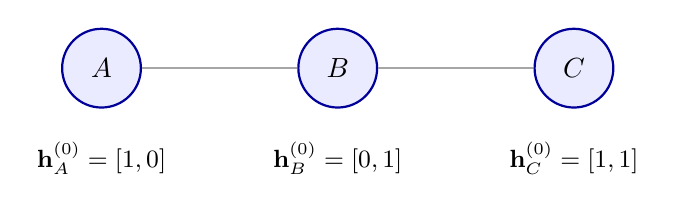
\begin{tikzpicture}[
    node/.style={circle, draw=blue!60!black, fill=blue!8, thick, minimum size=1.0cm, font=\bfseries},
    arr/.style={-, thick, gray!70}
]
    \node[node] (A) at (0,0) {$A$};
    \node[node] (B) at (3,0) {$B$};
    \node[node] (C) at (6,0) {$C$};
    \draw[arr] (A) -- (B);
    \draw[arr] (B) -- (C);
    \node[font=\small, below=0.3cm of A] {$\mathbf{h}_A^{(0)} = [1,0]$};
    \node[font=\small, below=0.3cm of B] {$\mathbf{h}_B^{(0)} = [0,1]$};
    \node[font=\small, below=0.3cm of C] {$\mathbf{h}_C^{(0)} = [1,1]$};
\end{tikzpicture}
\end{center}

The adjacency matrix is:
\[
\mathbf{A} = \begin{pmatrix} 0 & 1 & 0 \\ 1 & 0 & 1 \\ 0 & 1 & 0 \end{pmatrix}
\quad
(A=0,\; B=1,\; C=2 \text{ in 0-indexed notation})
\]

The neighbourhoods are: $\mathcal{N}(A) = \{B\}$, $\mathcal{N}(B) = \{A, C\}$, $\mathcal{N}(C) = \{B\}$.

We interpret the two-dimensional feature vector as $[\text{infected-flag},\; \text{recovered-flag}]$:
\begin{itemize}[noitemsep]
    \item Node $A$: observed as Infected ($\mathbf{h}_A^{(0)} = [1,0]$).
    \item Node $B$: observed as Recovered ($\mathbf{h}_B^{(0)} = [0,1]$).
    \item Node $C$: observed as both Infected and Recovered (think of a summary feature; $\mathbf{h}_C^{(0)} = [1,1]$).
\end{itemize}
\end{examplebox}

\subsection{Aggregation Function Comparison}

The choice of $\bigoplus$ is a design decision with real consequences:

\begin{itemize}
    \item \textbf{Mean aggregation}: $\mathbf{m}_v = \frac{1}{|\mathcal{N}(v)|}\sum_{u \in \mathcal{N}(v)} \mathbf{h}_u$. Captures the \emph{average} feature in the neighbourhood. Degree-invariant: a hub node and a leaf node that share the same single neighbour feature will produce the same aggregate. Useful when the relative proportion of feature types matters.
    \item \textbf{Sum aggregation}: $\mathbf{m}_v = \sum_{u \in \mathcal{N}(v)} \mathbf{h}_u$. Preserves the exact count of each feature type. A hub node with 10 infected neighbours aggregates to a much larger value than a leaf node with 1 infected neighbour. More expressive than mean (as proven by the GIN paper; see Section~\ref{sec:gin}).
    \item \textbf{Max aggregation}: $\mathbf{m}_v = \max_{u \in \mathcal{N}(v)} \mathbf{h}_u$ (element-wise). Captures the \emph{presence} of the most salient feature, but is blind to multiplicity. Useful for detecting whether \emph{any} neighbour has a specific property.
\end{itemize}

% =============================================================================
\section{Graph Convolutional Networks (GCN)}
% =============================================================================

The Graph Convolutional Network (GCN), introduced by Kipf \& Welling (2017), is the canonical starting point for graph deep learning. It provides an elegant, symmetric normalization of the message-passing operation.

\subsection{The GCN Update Rule}

\begin{mathbox}{GCN Layer}
The GCN layer computes:
\begin{equation}
    \mathbf{H}^{(l+1)} = \sigma\!\left(\tilde{\mathbf{D}}^{-1/2}\, \tilde{\mathbf{A}}\, \tilde{\mathbf{D}}^{-1/2}\, \mathbf{H}^{(l)}\, \mathbf{W}^{(l)}\right)
    \label{eq:gcn}
\end{equation}
where:
\begin{itemize}[noitemsep]
    \item $\mathbf{H}^{(l)} \in \mathbb{R}^{N \times d_l}$: the matrix of all $N$ node embeddings at layer $l$, stacked row-wise.
    \item $\tilde{\mathbf{A}} = \mathbf{A} + \mathbf{I}$: the adjacency matrix with \textbf{self-loops added}. Adding the identity matrix $\mathbf{I}$ ensures that each node includes its own features in its aggregation (otherwise, the update step only aggregates neighbours, forgetting the node's own current state).
    \item $\tilde{\mathbf{D}}$: the degree matrix of $\tilde{\mathbf{A}}$. $\tilde{D}_{vv} = \sum_j \tilde{A}_{vj}$ is the degree of node $v$ in $\tilde{\mathbf{A}}$ (i.e., its original degree plus 1 for the self-loop).
    \item $\tilde{\mathbf{D}}^{-1/2}$: the matrix whose diagonal entries are $\tilde{D}_{vv}^{-1/2} = 1/\sqrt{\tilde{D}_{vv}}$.
    \item $\mathbf{W}^{(l)} \in \mathbb{R}^{d_l \times d_{l+1}}$: a learnable weight matrix that projects the embedding from dimension $d_l$ to dimension $d_{l+1}$.
    \item $\sigma$: an element-wise non-linear activation (ReLU, PReLU, etc.).
\end{itemize}
\end{mathbox}

\subsection{Why the Symmetric Normalization $\tilde{\mathbf{D}}^{-1/2} \tilde{\mathbf{A}} \tilde{\mathbf{D}}^{-1/2}$?}

The raw sum $\tilde{\mathbf{A}} \mathbf{H}$ is problematic: high-degree nodes aggregate far more information than low-degree nodes, so their embeddings will have much larger magnitudes. This creates numerical instability and makes the network sensitive to the degree distribution.

The symmetric normalization $\hat{\mathbf{A}} = \tilde{\mathbf{D}}^{-1/2} \tilde{\mathbf{A}} \tilde{\mathbf{D}}^{-1/2}$ scales each entry $\tilde{A}_{uv}$ by $\frac{1}{\sqrt{\tilde{d}_u} \cdot \sqrt{\tilde{d}_v}}$, where $\tilde{d}_v$ is the degree of node $v$ in $\tilde{\mathbf{A}}$. This means:
\begin{itemize}[noitemsep]
    \item A message from a high-degree neighbour is down-weighted (large $\tilde{d}_u$ shrinks the coefficient).
    \item A high-degree target node also down-weights all incoming messages (large $\tilde{d}_v$ shrinks its received signals).
\end{itemize}
The result is a \emph{balanced} aggregation where no single high-degree node dominates the representation.

\begin{examplebox}{GCN Computation on the A--B--C Graph}
We compute $\hat{\mathbf{A}} = \tilde{\mathbf{D}}^{-1/2} \tilde{\mathbf{A}} \tilde{\mathbf{D}}^{-1/2}$ step by step.

\textbf{Step 1: Add self-loops.}
\[
\tilde{\mathbf{A}} = \mathbf{A} + \mathbf{I} =
\begin{pmatrix} 0 & 1 & 0 \\ 1 & 0 & 1 \\ 0 & 1 & 0 \end{pmatrix}
+
\begin{pmatrix} 1 & 0 & 0 \\ 0 & 1 & 0 \\ 0 & 0 & 1 \end{pmatrix}
=
\begin{pmatrix} 1 & 1 & 0 \\ 1 & 1 & 1 \\ 0 & 1 & 1 \end{pmatrix}
\]

\textbf{Step 2: Compute degree matrix $\tilde{\mathbf{D}}$.}
Row sums of $\tilde{\mathbf{A}}$: $\tilde{d}_A = 1+1+0 = 2$, $\tilde{d}_B = 1+1+1 = 3$, $\tilde{d}_C = 0+1+1 = 2$.
\[
\tilde{\mathbf{D}} = \begin{pmatrix} 2 & 0 & 0 \\ 0 & 3 & 0 \\ 0 & 0 & 2 \end{pmatrix}
\]

\textbf{Step 3: Compute $\tilde{\mathbf{D}}^{-1/2}$.}
\[
\tilde{\mathbf{D}}^{-1/2} = \begin{pmatrix} 1/\sqrt{2} & 0 & 0 \\ 0 & 1/\sqrt{3} & 0 \\ 0 & 0 & 1/\sqrt{2} \end{pmatrix}
\approx \begin{pmatrix} 0.707 & 0 & 0 \\ 0 & 0.577 & 0 \\ 0 & 0 & 0.707 \end{pmatrix}
\]

\textbf{Step 4: Compute $\hat{\mathbf{A}} = \tilde{\mathbf{D}}^{-1/2} \tilde{\mathbf{A}} \tilde{\mathbf{D}}^{-1/2}$.}
The entry $\hat{A}_{ij} = \frac{\tilde{A}_{ij}}{\sqrt{\tilde{d}_i} \cdot \sqrt{\tilde{d}_j}}$.

\medskip
\begin{center}
\renewcommand{\arraystretch}{1.5}
\begin{tabular}{c|ccc}
    & $A$ & $B$ & $C$ \\
\hline
$A$ & $\frac{1}{\sqrt{2}\cdot\sqrt{2}} = 0.500$ & $\frac{1}{\sqrt{2}\cdot\sqrt{3}} \approx 0.408$ & $\frac{0}{\cdots} = 0.000$ \\
$B$ & $\frac{1}{\sqrt{3}\cdot\sqrt{2}} \approx 0.408$ & $\frac{1}{\sqrt{3}\cdot\sqrt{3}} \approx 0.333$ & $\frac{1}{\sqrt{3}\cdot\sqrt{2}} \approx 0.408$ \\
$C$ & $\frac{0}{\cdots} = 0.000$ & $\frac{1}{\sqrt{2}\cdot\sqrt{3}} \approx 0.408$ & $\frac{1}{\sqrt{2}\cdot\sqrt{2}} = 0.500$ \\
\end{tabular}
\end{center}

\[
\hat{\mathbf{A}} \approx \begin{pmatrix} 0.500 & 0.408 & 0.000 \\ 0.408 & 0.333 & 0.408 \\ 0.000 & 0.408 & 0.500 \end{pmatrix}
\]

\textbf{Step 5: Multiply by feature matrix $\mathbf{H}^{(0)}$.}
\[
\mathbf{H}^{(0)} = \begin{pmatrix} 1 & 0 \\ 0 & 1 \\ 1 & 1 \end{pmatrix}
\]
\[
\hat{\mathbf{A}} \mathbf{H}^{(0)} \approx
\begin{pmatrix}
0.500 \cdot 1 + 0.408 \cdot 0 + 0.000 \cdot 1 & 0.500 \cdot 0 + 0.408 \cdot 1 + 0.000 \cdot 1 \\
0.408 \cdot 1 + 0.333 \cdot 0 + 0.408 \cdot 1 & 0.408 \cdot 0 + 0.333 \cdot 1 + 0.408 \cdot 1 \\
0.000 \cdot 1 + 0.408 \cdot 0 + 0.500 \cdot 1 & 0.000 \cdot 0 + 0.408 \cdot 1 + 0.500 \cdot 1
\end{pmatrix}
=
\begin{pmatrix} 0.500 & 0.408 \\ 0.816 & 0.741 \\ 0.500 & 0.908 \end{pmatrix}
\]

This intermediate result (before applying $\mathbf{W}^{(l)}$ and $\sigma$) shows what the normalized aggregation produces. Node $B$ now holds a larger signal because it received contributions from both $A$ and $C$ in addition to itself.
\end{examplebox}

\begin{keyinsight}{GCN as Spectral Graph Theory}
Kipf \& Welling derived the GCN update rule not from the message-passing intuition above, but from the spectral graph theory perspective. They showed that $\hat{\mathbf{A}} = \tilde{\mathbf{D}}^{-1/2} \tilde{\mathbf{A}} \tilde{\mathbf{D}}^{-1/2}$ is a first-order approximation of spectral graph convolution using the normalized graph Laplacian. This elegant connection means that GCN is implicitly performing a kind of smoothing on the graph signal---averaging each node's features with its neighbours, weighted by the inverse square root of their degrees.
\end{keyinsight}

% =============================================================================
\section{GraphSAGE: Sampling and Aggregating}
% =============================================================================

GCN has a serious scalability limitation: to compute the embedding of a single node, it must gather information from \emph{all} nodes in its $L$-hop neighbourhood. In a power-law social network, a hub node at layer 2 might require messages from millions of nodes. GraphSAGE (Hamilton, Ying \& Leskovec, 2017) addresses this with neighbourhood sampling.

\subsection{The Core Idea}

Instead of aggregating over the full neighbourhood $\mathcal{N}(v)$, GraphSAGE samples a fixed number $k$ of neighbours uniformly at random. This bounds the computational cost per node at each layer, regardless of degree.

More importantly, GraphSAGE introduces a key architectural change: instead of replacing the node's own embedding with the aggregated neighbour information, it \emph{concatenates} the two. This means the node always retains a direct memory of its own previous state.

\begin{mathbox}{GraphSAGE Update Rule}
At each layer $l$, GraphSAGE computes:
\begin{enumerate}[noitemsep]
    \item Sample a subset $\mathcal{S}(v) \subseteq \mathcal{N}(v)$ with $|\mathcal{S}(v)| = k$.
    \item Aggregate the sampled neighbours:
    \[
        \mathbf{m}_v^{(l)} = \text{MEAN}\!\left(\left\{\mathbf{h}_u^{(l-1)} : u \in \mathcal{S}(v)\right\}\right)
    \]
    \item Concatenate and apply a linear transformation with activation:
    \begin{equation}
        \mathbf{h}_v^{(l)} = \sigma\!\left(\mathbf{W}^{(l)} \cdot \left[\mathbf{h}_v^{(l-1)}\; \big\|\; \mathbf{m}_v^{(l)}\right]\right)
        \label{eq:sage}
    \end{equation}
\end{enumerate}
Here $\|$ denotes vector concatenation. The weight matrix $\mathbf{W}^{(l)}$ projects the concatenated vector $[\mathbf{h}_v^{(l-1)} \| \mathbf{m}_v^{(l)}] \in \mathbb{R}^{2d_{l-1}}$ to the output dimension $d_l$.
\end{mathbox}

\subsection{Why Concatenation Matters}

In GCN, the update $\mathbf{h}_v^{(l+1)} = \sigma(\hat{\mathbf{A}}_v \mathbf{H}^{(l)} \mathbf{W}^{(l)})$ implicitly mixes the node's own features with its neighbours' features through the self-loop (the $\mathbf{I}$ in $\tilde{\mathbf{A}}$). GraphSAGE makes this mixing explicit and asymmetric: the weight matrix sees both the node's own features and the neighbour aggregate as separate, independent inputs. This gives the model more freedom to decide how much to trust its own current state versus the neighbourhood signal.

In epidemic source detection, this is meaningful: the node's own observed state (Infected or Recovered) is direct evidence about its role in the outbreak. The neighbour aggregate provides indirect contextual evidence. Concatenating them lets the model weigh these two types of evidence independently.

\begin{examplebox}{GraphSAGE on A--B--C (Full Neighbourhood, No Sampling)}
For this small graph, sampling with $k=2$ is equivalent to using the full neighbourhood. Using $\mathbf{h}^{(0)} = \{[1,0], [0,1], [1,1]\}$ for $A, B, C$.

\medskip
\textbf{Node A:} $\mathcal{N}(A) = \{B\}$
\[
\mathbf{m}_A = \text{MEAN}\!\left(\{[0,1]\}\right) = [0.000,\, 1.000]
\]
\[
\left[\mathbf{h}_A^{(0)} \| \mathbf{m}_A\right] = [1.000,\; 0.000,\; 0.000,\; 1.000]
\]

\textbf{Node B:} $\mathcal{N}(B) = \{A, C\}$
\[
\mathbf{m}_B = \text{MEAN}\!\left(\{[1,0],\; [1,1]\}\right) = \left[\frac{1+1}{2},\; \frac{0+1}{2}\right] = [1.000,\; 0.500]
\]
\[
\left[\mathbf{h}_B^{(0)} \| \mathbf{m}_B\right] = [0.000,\; 1.000,\; 1.000,\; 0.500]
\]

\textbf{Node C:} $\mathcal{N}(C) = \{B\}$
\[
\mathbf{m}_C = \text{MEAN}\!\left(\{[0,1]\}\right) = [0.000,\, 1.000]
\]
\[
\left[\mathbf{h}_C^{(0)} \| \mathbf{m}_C\right] = [1.000,\; 1.000,\; 0.000,\; 1.000]
\]

The final embeddings $\mathbf{h}_v^{(1)} = \sigma(\mathbf{W}^{(0)} \cdot [\mathbf{h}_v^{(0)} \| \mathbf{m}_v])$ require a weight matrix $\mathbf{W}^{(0)} \in \mathbb{R}^{d_1 \times 4}$, which is learned during training. Observe that node $B$'s input vector $[0, 1, 1, 0.5]$ is distinct from both $A$'s $[1, 0, 0, 1]$ and $C$'s $[1, 1, 0, 1]$, even though $A$ and $C$ are structurally similar (both have degree 1 in the original graph). The concatenation of the node's own features breaks this symmetry.
\end{examplebox}

% =============================================================================
\section{Graph Attention Networks (GAT)}
% =============================================================================

GCN normalizes the aggregation by node degree---a fixed, structural quantity. GraphSAGE uses uniform mean over sampled neighbours. But not all neighbours are equally informative. In an epidemic network, if node $v$ is Susceptible and one of its neighbours $u$ is Infected while another neighbour $w$ is also Susceptible, the message from $u$ is far more diagnostic for source detection than the message from $w$.

The Graph Attention Network (GAT), introduced by Veli{\v{c}}kovi{\'c} et al.\ (2018), learns to assign different \emph{attention weights} to different neighbours.

\subsection{Attention Coefficient Computation}

\begin{mathbox}{GAT Layer}
Let $\mathbf{h}_v^{(l-1)} \in \mathbb{R}^{d}$ be the embedding of node $v$ before the current layer. GAT computes:

\textbf{Step 1: Linear projection.} Project all node embeddings to a shared space:
\[
\mathbf{z}_v = \mathbf{W} \mathbf{h}_v^{(l-1)}, \quad \mathbf{z}_v \in \mathbb{R}^{d'}
\]

\textbf{Step 2: Unnormalized attention.} For each edge $(v, w)$, compute a scalar attention score using a learnable attention vector $\mathbf{a} \in \mathbb{R}^{2d'}$:
\begin{equation}
    e_{vw} = \text{LeakyReLU}\!\left(\mathbf{a}^\top\!\left[\mathbf{z}_v \| \mathbf{z}_w\right]\right)
    \label{eq:gat_attn}
\end{equation}
The concatenation $[\mathbf{z}_v \| \mathbf{z}_w] \in \mathbb{R}^{2d'}$ captures both the sender's and receiver's current representations.

\textbf{Step 3: Normalize with softmax.} Normalize the attention scores over all neighbours of $v$ to obtain coefficients that sum to 1:
\begin{equation}
    \alpha_{vw} = \frac{\exp(e_{vw})}{\sum_{u \in \mathcal{N}(v)} \exp(e_{vu})}
    \label{eq:gat_softmax}
\end{equation}

\textbf{Step 4: Weighted aggregation.}
\begin{equation}
    \mathbf{h}_v^{(l)} = \sigma\!\left(\sum_{w \in \mathcal{N}(v)} \alpha_{vw}\, \mathbf{W} \mathbf{h}_w^{(l-1)}\right)
    \label{eq:gat_update}
\end{equation}
\end{mathbox}

\begin{examplebox}{GAT Attention on a Two-Node Graph}
Consider two nodes $v$ and $w$ with scalar (1-dimensional) features $h_v = 2.0$ and $h_w = 0.5$. The graph has one edge $v \to w$ (self-loops included). Let $W = 0.5$ (scalar projection) and attention vector $\mathbf{a} = [1, 1]^\top$.

\textbf{Projections:} $z_v = 0.5 \cdot 2.0 = 1.0$, $z_w = 0.5 \cdot 0.5 = 0.25$.

\textbf{Unnormalized scores} (including self-loop for $v$):
\begin{align*}
    e_{v \leftarrow v} &= \text{LeakyReLU}([1,1]^\top [1.0, 1.0]) = \text{LeakyReLU}(2.0) = 2.0 \\
    e_{v \leftarrow w} &= \text{LeakyReLU}([1,1]^\top [1.0, 0.25]) = \text{LeakyReLU}(1.25) = 1.25
\end{align*}

\textbf{Normalized coefficients:}
\[
\alpha_{v \leftarrow v} = \frac{e^{2.0}}{e^{2.0} + e^{1.25}} = \frac{7.389}{7.389 + 3.490} \approx 0.679
\]
\[
\alpha_{v \leftarrow w} = \frac{e^{1.25}}{e^{2.0} + e^{1.25}} \approx \frac{3.490}{10.879} \approx 0.321
\]

\textbf{Interpretation:} Node $v$, which has a higher feature value (and hence a stronger self-projection), assigns 67.9\% of its attention to itself and 32.1\% to its neighbour $w$. A learned attention mechanism can adjust these weights based on contextual patterns across the whole training set.
\end{examplebox}

\subsection{Multi-Head Attention}

A single attention head may not capture all the relevant relationships. GAT uses $K$ independent attention mechanisms (heads), each with its own parameters $\mathbf{W}_k$ and $\mathbf{a}_k$:

\begin{equation}
    \mathbf{h}_v^{(l)} = \Big\|_{k=1}^{K}\, \sigma\!\left(\sum_{w \in \mathcal{N}(v)} \alpha_{vw}^k\, \mathbf{W}_k\, \mathbf{h}_w^{(l-1)}\right)
    \label{eq:gat_multihead}
\end{equation}

The $K$ outputs are concatenated (operator $\|$). For the final layer, they are averaged instead to keep the output dimension fixed:
$\mathbf{h}_v^{(L)} = \sigma\!\left(\frac{1}{K}\sum_{k=1}^K \sum_{w \in \mathcal{N}(v)} \alpha_{vw}^k \mathbf{W}_k \mathbf{h}_w^{(L-1)}\right)$.

\begin{keyinsight}{Why Multi-Head Attention?}
Different heads can specialise in different structural patterns. One head might learn to up-weight infected neighbours; another might learn to down-weight high-degree hubs (which are noisy aggregators). The concatenation of all heads gives the model a richer view of the neighbourhood than any single weighting scheme. This is exactly analogous to multi-head attention in Transformers---GAT can be understood as a Transformer where the attention is restricted to the graph neighbourhood rather than the full sequence.
\end{keyinsight}

% =============================================================================
\section{Graph Isomorphism Networks (GIN)}
\label{sec:gin}
% =============================================================================

GCN, GraphSAGE, and GAT are all powerful in practice, but they share a theoretical weakness: there exist pairs of non-isomorphic graphs (graphs that look different but cannot be distinguished by degree-sequence counting) that all three architectures map to identical embeddings. This means they provably cannot solve certain graph classification problems.

The Graph Isomorphism Network (GIN), introduced by Xu et al.\ (2019), is designed to be as expressive as theoretically possible within the MPNN class.

\subsection{The Weisfeiler-Lehman Test Connection}

The \emph{Weisfeiler-Lehman (WL) graph isomorphism test} is a classical algorithm that iteratively assigns colour labels to nodes based on their neighbourhood. Two graphs are declared non-isomorphic if, at any iteration, their colour histograms differ. Xu et al.\ proved that:

\begin{itemize}[noitemsep]
    \item Any MPNN is at most as powerful as the WL test at distinguishing non-isomorphic graphs.
    \item GIN achieves this theoretical maximum---it is \emph{as powerful as the WL test} among all MPNNs.
\end{itemize}

The key insight: the WL test uses injective aggregation (each distinct multiset of neighbourhood colours maps to a distinct new colour). For an MPNN to be similarly injective, its aggregation must be injective over multisets. \textbf{Sum aggregation is injective over multisets; mean and max are not.}

\subsection{The GIN Update Rule}

\begin{mathbox}{GIN Layer}
\begin{equation}
    \mathbf{h}_v^{(l)} = \text{MLP}^{(l)}\!\left((1 + \varepsilon^{(l)})\, \mathbf{h}_v^{(l-1)} + \sum_{u \in \mathcal{N}(v)} \mathbf{h}_u^{(l-1)}\right)
    \label{eq:gin}
\end{equation}
where:
\begin{itemize}[noitemsep]
    \item $\text{MLP}^{(l)}$ is a multi-layer perceptron (at least 2 layers, to ensure the final aggregation function is injective on the combined argument).
    \item $\varepsilon^{(l)}$ is a scalar---either a learnable parameter or a fixed constant (e.g., 0). It controls how much the model weights its own previous embedding relative to the neighbourhood sum.
    \item The use of \textbf{SUM} (not mean, not max) is the critical design choice.
\end{itemize}
\end{mathbox}

\subsection{Why SUM and Not Mean?}

To understand why sum is necessary, consider two cases:
\begin{itemize}
    \item Node $v_1$ has two neighbours, both with feature $[1]$. Neighbourhood sum $= 2$. Neighbourhood mean $= 1$.
    \item Node $v_2$ has one neighbour with feature $[1]$. Neighbourhood sum $= 1$. Neighbourhood mean $= 1$.
\end{itemize}
Mean aggregation cannot distinguish $v_1$ from $v_2$. Sum aggregation distinguishes them trivially. In an epidemic context, a node with two infected neighbours is a very different situation from a node with one infected neighbour---sum aggregation preserves this critical multiplicity.

\begin{examplebox}{GIN on A--B--C with $\varepsilon = 0$}
Using $\mathbf{h}^{(0)} = \{A=[1,0],\; B=[0,1],\; C=[1,1]\}$ and $\varepsilon = 0$ for simplicity.

\textbf{Node A:}
$(1+0)\cdot[1,0] + \sum_{u \in \{B\}} [0,1] = [1,0] + [0,1] = [1,1]$

\textbf{Node B:}
$(1+0)\cdot[0,1] + \sum_{u \in \{A,C\}} ([1,0]+[1,1]) = [0,1] + [2,1] = [2,2]$

\textbf{Node C:}
$(1+0)\cdot[1,1] + \sum_{u \in \{B\}} [0,1] = [1,1] + [0,1] = [1,2]$

The three pre-MLP vectors are $[1,1]$, $[2,2]$, $[1,2]$---all distinct. After applying $\text{MLP}^{(0)}$, the model can map these to any desired output embeddings. Note that the sum aggregation for node $B$ correctly reflects that it received two neighbour messages ($A$ and $C$), not just an average.
\end{examplebox}

% =============================================================================
\section{Over-Smoothing: When Depth Becomes a Liability}
% =============================================================================

In standard deep learning, adding more layers typically improves performance up to a point. In GNNs, there is a sharp pathological threshold: stack too many layers and all node embeddings become identical. This phenomenon is called \textbf{over-smoothing}.

\subsection{The Mechanism}

Consider what happens to the aggregated feature matrix $\hat{\mathbf{A}}^L \mathbf{H}^{(0)}$ as $L \to \infty$. The matrix $\hat{\mathbf{A}} = \tilde{\mathbf{D}}^{-1/2} \tilde{\mathbf{A}} \tilde{\mathbf{D}}^{-1/2}$ is a real symmetric matrix with eigenvalues in $(-1, 1]$. Repeated multiplication by $\hat{\mathbf{A}}$ drives all eigencomponents except the largest toward zero. The result is that every node's representation converges to a fixed point proportional to its degree---all node embeddings in the same connected component become equal.

\begin{analogybox}{Everything Becomes Gray When You Average Enough}
Imagine a painting made of thousands of coloured tiles. If you replace each tile's colour with the average colour of it and its neighbours, then repeat this process 50 times, the painting becomes a uniform gray---all the fine structure is washed out.

A GNN with too many layers does exactly the same thing to node embeddings. After enough rounds of neighbourhood averaging, every node's representation reflects the global average of all node features, and no node is distinguishable from any other.
\end{analogybox}

\subsection{Empirical Behavior Across Depths}

The following table illustrates the expected decay of embedding variance (a proxy for discriminative power) as the number of GNN layers increases on a typical sparse graph:

\begin{center}
\renewcommand{\arraystretch}{1.4}
\begin{tabular}{ccc}
\toprule
\textbf{Layers $L$} & \textbf{Relative Embedding Variance} & \textbf{Effective Receptive Field} \\
\midrule
1 & $\approx 1.00$ (high, local features) & Immediate neighbours \\
2 & $\approx 0.72$ & 2-hop neighbourhood \\
4 & $\approx 0.31$ & 4-hop neighbourhood \\
8 & $\approx 0.05$ & Most of the graph (small-world) \\
16+ & $\approx 0.00$ & Entire graph (fully smoothed) \\
\bottomrule
\end{tabular}
\end{center}

This suggests a practical design principle: for source detection on networks with diameter $D$, we want $L \approx D/2$ to $D$ layers---enough to see the whole affected region, but not so many that all information is destroyed.

\subsection{Mitigation Strategies}

\begin{conceptbox}{Three Strategies Against Over-Smoothing}

\textbf{1. Skip (Residual) Connections.} Borrow from ResNets: add the input to the layer's output, $\mathbf{h}_v^{(l+1)} = \mathbf{h}_v^{(l)} + \text{GNN-layer}(\mathbf{h}_v^{(l)})$. The gradient now has a direct path back to early layers, and the model can learn to \emph{not} aggregate if aggregation is harmful. Our \texttt{StaticGNN} uses a global skip connection where the raw input features $\mathbf{x}$ are concatenated directly to the final layer's input, ensuring the model retains direct access to the original observations.

\textbf{2. PairNorm.} A dedicated normalization technique (Zhao \& Akoglu, 2020) that centers node embeddings and rescales them to a fixed total squared norm after each layer, explicitly preventing the collapse to a constant. It is more targeted than batch normalization for this specific problem.

\textbf{3. DropEdge.} Randomly drop edges from the input graph at each training step (Rong et al., 2020). This slows information propagation, acts as data augmentation, and reduces the speed of over-smoothing. It also improves robustness to missing edges, which is directly relevant when contact network data is incomplete.
\end{conceptbox}

% =============================================================================
\section{PyTorch Geometric: The Engineering Layer}
% =============================================================================

The mathematics of GNNs is elegant, but implementing them efficiently on modern hardware requires careful engineering. PyTorch Geometric (PyG, Fey \& Lenssen, 2019) is the standard library for this. It provides efficient sparse representations, a flexible base class for message passing, and utilities for batching variable-size graphs.

\subsection{The COO Sparse Format: \texttt{edge\_index}}

An adjacency matrix $\mathbf{A} \in \mathbb{R}^{N \times N}$ is $O(N^2)$ in memory. For a network with 10,000 nodes and 50,000 edges, the dense matrix would require $10^8$ entries---almost all of which are zero. PyG uses the \textbf{Coordinate (COO) format} to represent graphs.

\begin{mathbox}{\texttt{edge\_index}: The COO Graph Representation}
In COO format, the graph topology is stored as two 1D integer arrays of length $|E|$ (number of directed edges):
\begin{itemize}[noitemsep]
    \item \texttt{edge\_index[0]}: the \textbf{source} (sender) node index for each edge.
    \item \texttt{edge\_index[1]}: the \textbf{destination} (receiver) node index for each edge.
\end{itemize}
The combined tensor has shape \texttt{[2, |E|]}. The $i$-th column $[\texttt{edge\_index[0,i]},\, \texttt{edge\_index[1,i]}]$ encodes a single directed edge.
\end{mathbox}

\begin{examplebox}{COO Encoding of the A--B--C Path Graph}
Label $A=0$, $B=1$, $C=2$. The undirected graph has edges $\{A\text{-}B, B\text{-}C\}$. In PyG, undirected edges are stored as two directed edges each:

\begin{center}
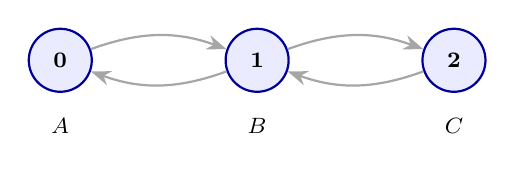
\begin{tikzpicture}[
    node/.style={circle, draw=blue!60!black, fill=blue!8, thick, minimum size=0.8cm, font=\footnotesize\bfseries},
    arr/.style={-{Stealth[length=2.5mm]}, thick, gray!70}
]
    \node[node] (A) at (0,0) {0};
    \node[node] (B) at (2.5,0) {1};
    \node[node] (C) at (5,0) {2};
    \node[font=\footnotesize, below=0.2cm of A] {$A$};
    \node[font=\footnotesize, below=0.2cm of B] {$B$};
    \node[font=\footnotesize, below=0.2cm of C] {$C$};
    \draw[arr, bend left=20] (A) to (B);
    \draw[arr, bend left=20] (B) to (A);
    \draw[arr, bend left=20] (B) to (C);
    \draw[arr, bend left=20] (C) to (B);
\end{tikzpicture}
\end{center}

\begin{lstlisting}[language=Python]
import torch
from torch_geometric.data import Data

# Edge list for path A-B-C (both directions)
edge_index = torch.tensor([
    [0, 1, 1, 2],  # sources:      A->B, B->A, B->C, C->B
    [1, 0, 2, 1],  # destinations: A->B, B->A, B->C, C->B
], dtype=torch.long)   # shape: [2, 4]

# Node features: [infected_flag, recovered_flag]
x = torch.tensor([
    [1, 0],  # Node A: Infected
    [0, 1],  # Node B: Recovered
    [1, 1],  # Node C: both
], dtype=torch.float)   # shape: [3, 2]

# Ground-truth source (for supervised training)
y = torch.tensor([0], dtype=torch.long)  # Node A is the source

# Create a PyG Data object
graph = Data(x=x, edge_index=edge_index, y=y)
print(graph)
# Data(x=[3, 2], edge_index=[2, 4], y=[1])
\end{lstlisting}

Why store both directions? PyG's \texttt{MessagePassing} base class propagates messages along directed edges. For an undirected aggregation (where $v$ receives from $u$ and $u$ receives from $v$), we must explicitly store both $u \to v$ and $v \to u$.
\end{examplebox}

\subsection{Edge Weights}

Many graphs carry edge weights---for example, the number of times two people contacted each other in a temporal network, or the probability that a contact was infectious. PyG supports edge attributes via the \texttt{edge\_attr} field of a \texttt{Data} object, and most convolution layers (including \texttt{GraphConv} used in our codebase) accept an optional \texttt{edge\_weight} argument.

\subsection{The \texttt{MessagePassing} Base Class}

PyG provides the \texttt{torch\_geometric.nn.MessagePassing} abstract base class that handles the bookkeeping of COO-format message passing. To implement a custom GNN layer, you subclass it and override three methods:

\begin{codewalk}{Implementing a Custom GNN Layer with MessagePassing}
\begin{lstlisting}[language=Python]
from torch_geometric.nn import MessagePassing
from torch.nn import Linear
import torch.nn.functional as F

class CustomGNNLayer(MessagePassing):
    def __init__(self, in_channels: int, out_channels: int,
                 aggr: str = 'add'):
        # aggr can be 'add', 'mean', or 'max'
        super().__init__(aggr=aggr)
        self.lin = Linear(in_channels, out_channels)

    def forward(self, x, edge_index, edge_weight=None):
        # Trigger the message-passing pipeline:
        # 1. Call message() for each edge
        # 2. Aggregate messages per target node
        # 3. Call update() on each node's aggregated message
        return self.propagate(edge_index, x=x,
                               edge_weight=edge_weight)

    def message(self, x_j, edge_weight):
        # x_j: features of the SOURCE node for each edge
        # Shape: [num_edges, in_channels]
        if edge_weight is not None:
            return edge_weight.view(-1, 1) * x_j
        return x_j

    def update(self, aggr_out):
        # aggr_out: the aggregated message for each TARGET node
        # Shape: [num_nodes, in_channels]
        return F.relu(self.lin(aggr_out))
\end{lstlisting}

The \texttt{propagate()} call orchestrates the entire pipeline. PyG automatically:
\begin{itemize}[noitemsep]
    \item Looks up the source node features for each edge (\texttt{x\_j} in \texttt{message()}).
    \item Routes messages to target nodes and applies the chosen \texttt{aggr} function.
    \item Passes the result to \texttt{update()}.
\end{itemize}
All of this is implemented internally as vectorized scatter operations on the GPU.
\end{codewalk}

\subsection{Batching Variable-Size Graphs}

One of PyG's most important engineering contributions is its batching strategy. Standard neural networks batch samples by stacking them into larger tensors (e.g., images into a $[B, C, H, W]$ tensor). Graphs cannot be stacked because they have different numbers of nodes and edges.

\begin{conceptbox}{PyG Batching: The Super-Graph Trick}
PyG batches $B$ graphs $G_1, G_2, \ldots, G_B$ by merging them into a single \textbf{disconnected super-graph}. Node indices are offset so that the $B$ sub-graphs do not share any nodes.

Concretely:
\begin{itemize}[noitemsep]
    \item All node feature matrices $\mathbf{X}_1, \ldots, \mathbf{X}_B$ are vertically concatenated: $\mathbf{X} = [\mathbf{X}_1; \mathbf{X}_2; \ldots; \mathbf{X}_B]$, giving a matrix of shape $[(N_1 + \cdots + N_B) \times F]$.
    \item All \texttt{edge\_index} tensors are offset and horizontally concatenated, with the edge index for graph $i$ shifted by $\sum_{j<i} N_j$.
    \item A \texttt{batch} vector of length $\sum N_i$ records which super-graph node belongs to which original graph: $\texttt{batch}[k] = i$ if node $k$ is in graph $G_i$.
\end{itemize}
Message passing on the super-graph is mathematically identical to independent message passing on each sub-graph, because there are no edges between sub-graphs.

\begin{lstlisting}[language=Python]
from torch_geometric.loader import DataLoader

dataset = [graph_1, graph_2, graph_3]  # list of Data objects
loader  = DataLoader(dataset, batch_size=2, shuffle=True)

for batch in loader:
    # batch.x:          shape [N1+N2, F]  -- all node features
    # batch.edge_index: shape [2, E1+E2]  -- all edges
    # batch.batch:      shape [N1+N2]     -- graph membership
    # batch.y:          shape [2]         -- one label per graph
    print(batch.batch)  # e.g., tensor([0, 0, 0, 1, 1])
\end{lstlisting}
\end{conceptbox}

The \texttt{batch} vector is crucial for the \textbf{readout} step, where we aggregate node-level embeddings into a single graph-level prediction. The \texttt{StaticGNN} uses it directly to reshape its final output (see the next section).

% =============================================================================
\section{Code Walkthrough: The \texttt{StaticGNN} in \texttt{gnn/static\_gnn.py}}
% =============================================================================

The \texttt{StaticGNN} is the baseline GNN model in this thesis. It treats the temporal contact network as a single static weighted graph, ignoring the temporal ordering of contacts. Understanding it in detail prepares us for the more sophisticated temporal architectures discussed in later chapters.

The architecture follows a three-stage design:
\[
\underbrace{\text{Preprocessing MLP}}_{\text{feature embedding}} \;\longrightarrow\; \underbrace{\text{Graph Convolution Stack}}_{\text{structural aggregation}} \;\longrightarrow\; \underbrace{\text{Postprocessing MLP} + \text{Final Layer}}_{\text{source scoring}}
\]

\subsection{Constructor and Layer Initialization}

\begin{codewalk}{StaticGNN: Constructor Overview}
\begin{lstlisting}[language=Python]
class StaticGNN(torch.nn.Module):
    def __init__(self,
                 num_preprocess_layers,   # int: depth of input MLP
                 embed_dim_preprocess,    # int: width of input MLP
                 num_postprocess_layers,  # int: depth of output MLP
                 num_conv_layers,         # int: number of GNN layers
                 aggr,                    # str: 'add', 'mean', or 'max'
                 num_node_features,       # int: F (raw feature dim)
                 hidden_channels,         # int: d (conv embedding dim)
                 num_classes,             # int: N (number of nodes)
                 dropout_rate,            # float: dropout probability p
                 batch_norm,              # bool: use BatchNorm1d?
                 skip):                   # bool: use skip connection?
\end{lstlisting}
Every hyperparameter is passed explicitly (no hardcoded values), and all are logged via wandb at training time. This design makes the model fully reproducible from a YAML config file.
\end{codewalk}

The constructor builds four sub-networks:

\begin{codewalk}{StaticGNN: Building the Four Sub-Networks}
\begin{lstlisting}[language=Python]
        # --- 1. PREPROCESSING MLP ---
        self.preprocess = torch.nn.Sequential()
        for l in range(num_preprocess_layers):
            in_features = (num_node_features if l == 0
                           else embed_dim_preprocess)
            self.preprocess.append(Linear(in_features,
                                          embed_dim_preprocess))
            if batch_norm:
                self.preprocess.append(
                    torch.nn.BatchNorm1d(embed_dim_preprocess))
            self.preprocess.append(torch.nn.PReLU())
            self.preprocess.append(torch.nn.Dropout(p=dropout_rate))

        # --- 2. GRAPH CONVOLUTION STACK ---
        self.convs  = torch.nn.ModuleList()
        self.banor  = torch.nn.ModuleList()   # BN for each conv layer
        self.activ  = torch.nn.ModuleList()   # PReLU for each conv layer
        for l in range(num_conv_layers):
            in_channels = (
                num_node_features       if (num_preprocess_layers==0
                                             and l==0)
                else embed_dim_preprocess if (num_preprocess_layers>0
                                               and l==0)
                else hidden_channels
            )
            self.convs.append(GraphConv(in_channels,
                                        hidden_channels, aggr=aggr))
            if batch_norm:
                self.banor.append(
                    torch.nn.BatchNorm1d(hidden_channels))
            self.activ.append(torch.nn.PReLU())

        # --- 3. POSTPROCESSING MLP ---
        self.postprocess = torch.nn.Sequential()
        for _ in range(num_postprocess_layers):
            self.postprocess.append(Linear(hidden_channels,
                                           hidden_channels))
            if batch_norm:
                self.postprocess.append(
                    torch.nn.BatchNorm1d(hidden_channels))
            self.postprocess.append(torch.nn.PReLU())
            self.postprocess.append(torch.nn.Dropout(p=dropout_rate))

        # --- 4. FINAL LAYER (with optional skip connection) ---
        in_channels = ((hidden_channels + num_node_features)
                       if skip else hidden_channels)
        self.final = torch.nn.Sequential()
        self.final.append(Linear(in_channels, 1))
        if batch_norm:
            self.final.append(torch.nn.BatchNorm1d(1))
        self.final.append(torch.nn.PReLU())
\end{lstlisting}
\end{codewalk}

\subsection{Design Decisions Worth Noting}

\begin{itemize}
    \item \textbf{\texttt{GraphConv}, not \texttt{GCNConv}}: the model uses PyG's \texttt{torch\_geometric.nn.GraphConv}, which differs slightly from the original GCN. \texttt{GraphConv} computes $\mathbf{h}_v' = \mathbf{W}_1 \mathbf{h}_v + \mathbf{W}_2 \sum_{u \in \mathcal{N}(v)} e_{uv} \mathbf{h}_u$ with \emph{separate} weight matrices for the self-term and the neighbour-aggregate term, giving it more expressive power than the symmetric normalization of plain GCN. Edge weights $e_{uv}$ are passed as \texttt{edge\_weights} in the forward pass.
    \item \textbf{\texttt{ModuleList} for conv/bn/activ}: the preprocessing and postprocessing stages use \texttt{torch.nn.Sequential} (which is convenient for fixed pipelines), but the convolution stack uses separate \texttt{ModuleList} objects for the conv layers, batch-norm layers, and activations. This is because \texttt{GraphConv} requires the \texttt{edge\_index} and \texttt{edge\_weights} arguments that \texttt{Sequential} cannot pass automatically.
    \item \textbf{Output dimension = 1}: the final linear layer outputs a single scalar per node, \emph{before} the reshape. This scalar is a raw unnormalized score for ``is this node the source?''
\end{itemize}

\subsection{Forward Pass with Shape Annotations}

\begin{codewalk}{StaticGNN: Forward Pass}
\begin{lstlisting}[language=Python]
    def forward(self, x, edge_index, edge_weights, batch):
        # x:            [total_nodes, F]       raw node features
        # edge_index:   [2, total_edges]        COO edge list
        # edge_weights: [total_edges]           scalar per edge
        # batch:        [total_nodes]           graph membership

        # ---- Stage 1: Preprocessing MLP ----
        x1 = self.preprocess(x)
        # x1: [total_nodes, embed_dim_preprocess]

        # ---- Stage 2: Graph Convolution Stack ----
        for i, conv in enumerate(self.convs):
            x1 = conv(x1, edge_index, edge_weights)
            # x1: [total_nodes, hidden_channels]
            if self.batch_norm:
                x1 = self.banor[i](x1)
            x1 = self.activ[i](x1)
            x1 = F.dropout(x1, p=self.dropout_rate,
                           training=self.training)

        # ---- Stage 3: Postprocessing MLP ----
        x1 = self.postprocess(x1)
        # x1: [total_nodes, hidden_channels]

        # ---- Stage 4: Final Layer + Reshape ----
        if self.skip:
            # Concatenate raw input features with learned embedding
            x1 = self.final(torch.cat([x, x1], dim=-1))
            # cat input:  [total_nodes, F + hidden_channels]
            # final output: [total_nodes, 1]
        else:
            x1 = self.final(x1)
            # x1: [total_nodes, 1]

        # Reshape from super-graph format to batch format:
        # [total_nodes, 1] --> [batch_size, num_classes]
        # where num_classes = N (nodes per graph)
        x1 = x1.reshape((batch.unique().shape[0], self.num_classes))
        # x1: [batch_size, N]

        # ---- Stage 5: Output Log-Probabilities ----
        x1 = F.log_softmax(x1, dim=1)
        # x1: [batch_size, N]  -- log-probabilities over source nodes
        return x1
\end{lstlisting}
\end{codewalk}

\begin{keyinsight}{The Reshape Trick and Why It Works}
The forward pass assumes that every graph in the batch has the same number of nodes $N$. This is guaranteed by the data generation pipeline (all simulations run on the same fixed network). Given this, the super-graph node features tensor of shape \texttt{[batch\_size $\times$ N, 1]} can be safely reshaped to \texttt{[batch\_size, N]}.

This allows the \texttt{log\_softmax} on \texttt{dim=1} to normalize over all $N$ nodes of each graph independently---producing, for each training example (epidemic snapshot), a proper probability distribution over which of the $N$ nodes was the source.

If graphs had different sizes, this reshape would be invalid. Handling variable-size readouts requires PyG's \texttt{global\_mean\_pool} or \texttt{global\_add\_pool} functions, which use the \texttt{batch} vector for graph-level aggregation.
\end{keyinsight}

\subsection{The Skip Connection}

The skip connection in \texttt{StaticGNN} is a global shortcut: the raw input features $\mathbf{x}$ (before any preprocessing or graph convolution) are concatenated to the deep embedding $\mathbf{x}_1$ just before the final classification layer.

\begin{center}
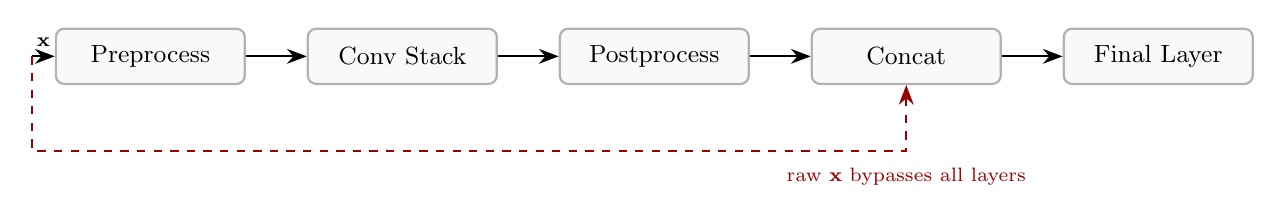
\begin{tikzpicture}[
    box/.style={rectangle, draw=gray!60, fill=gray!5, rounded corners=3pt, thick,
                minimum width=2.4cm, minimum height=0.7cm, font=\small},
    arr/.style={-{Stealth[length=2.5mm]}, thick},
    skip/.style={-{Stealth[length=2.5mm]}, thick, red!60!black, dashed}
]
    \node[box] (pre)    at (0, 0)    {Preprocess};
    \node[box] (conv)   at (3.2, 0)  {Conv Stack};
    \node[box] (post)   at (6.4, 0)  {Postprocess};
    \node[box] (cat)    at (9.6, 0)  {Concat};
    \node[box] (final)  at (12.8, 0) {Final Layer};

    \draw[arr] (-1.5, 0) -- (pre)  node[midway, above, font=\scriptsize]{$\mathbf{x}$};
    \draw[arr] (pre) -- (conv);
    \draw[arr] (conv) -- (post);
    \draw[arr] (post) -- (cat);
    \draw[arr] (cat) -- (final);

    % Skip connection
    \draw[skip] (-1.5, 0) -- (-1.5, -1.2) -- (9.6, -1.2) -- (cat)
        node[midway, below, font=\scriptsize, below=0.5cm]{raw $\mathbf{x}$ bypasses all layers};
\end{tikzpicture}
\end{center}

\textbf{Why does this help?} After $L$ rounds of message passing and non-linear projection, the embedding $\mathbf{x}_1$ captures rich structural context but may have diluted the original node-level observation (whether this specific node was seen as Infected or Recovered). The skip connection forces the model to always have direct access to these raw observations, which are strong single-node evidence for or against being the source. The combined vector $[\mathbf{x} \| \mathbf{x}_1]$ lets the final linear layer perform a weighted combination of structural evidence and direct observational evidence.

\subsection{YAML Configuration Mapping}

The \texttt{StaticGNN} is never instantiated with hardcoded arguments. A typical experiment configuration looks like:

\begin{codewalk}{YAML Configuration for StaticGNN}
\begin{lstlisting}[language={}]
gnn:
  conv_type: GraphConv      # which PyG conv to use
  hidden_dim: 64            # hidden_channels
  n_layers: 4               # num_conv_layers
  aggr: add                 # aggregation: 'add', 'mean', or 'max'
  num_preprocess_layers: 2
  embed_dim_preprocess: 64
  num_postprocess_layers: 1
  dropout_rate: 0.2
  batch_norm: true
  skip: true
\end{lstlisting}
With \texttt{n\_layers: 4} and a typical network diameter of 6--8, this configuration allows the model to gather evidence from approximately a 4-hop radius around each candidate source node---covering most of the observable outbreak footprint without reaching the over-smoothing regime.
\end{codewalk}

% =============================================================================
\section{Summary and Connection to the Thesis}
% =============================================================================

This chapter has built the complete toolkit for graph-based deep learning:

\begin{enumerate}
    \item \textbf{Why graphs need special architectures}: MLPs cannot handle variable size or graph structure; CNNs require a regular grid that graphs lack.
    \item \textbf{The MPNN framework}: a unified language for message generation, aggregation, and update that subsumes GCN, GraphSAGE, GAT, and GIN.
    \item \textbf{GCN}: symmetric normalization by degree prevents magnitude explosion; $\tilde{\mathbf{D}}^{-1/2}\tilde{\mathbf{A}}\tilde{\mathbf{D}}^{-1/2}$ is the workhorse of the field.
    \item \textbf{GraphSAGE}: neighbourhood sampling for scalability; concatenation for preserving node identity.
    \item \textbf{GAT}: learned attention weights that can identify the most diagnostic neighbours; multi-head attention for robustness.
    \item \textbf{GIN}: sum aggregation and MLP update for maximum expressiveness within the WL hierarchy.
    \item \textbf{Over-smoothing}: depth is a double-edged sword; skip connections, PairNorm, and DropEdge are the standard mitigations.
    \item \textbf{PyTorch Geometric}: COO format, the \texttt{MessagePassing} base class, and the super-graph batching trick.
    \item \textbf{StaticGNN}: a configurable Preprocess $\to$ GraphConv Stack $\to$ Postprocess $\to$ Skip-augmented readout architecture, implemented in \texttt{gnn/static\_gnn.py}.
\end{enumerate}

\begin{keyinsight}{What the StaticGNN Cannot See}
The \texttt{StaticGNN} is a strong baseline precisely because it already has all the machinery described in this chapter. Its fundamental limitation is the word ``Static'': it projects all temporal contact events onto a single aggregated network, losing the information about \emph{when} each contact occurred. Two contact sequences that produce identical aggregate networks---but where the temporal ordering implies completely different possible epidemic paths---will produce identical model inputs.

This is the core motivation for the temporal architectures in subsequent chapters: the De Bruijn GNN (Chapter~10), which encodes causal walks as higher-order nodes, and the DAG-GNN on Temporal Event Graphs (Chapter~11), which preserves the arrow of time explicitly in the graph structure.
\end{keyinsight}

\begin{paperbox}{Key Papers for This Chapter}
\begin{itemize}
    \item \textbf{Kipf \& Welling (2017)} --- ``Semi-Supervised Classification with Graph Convolutional Networks'' (ICLR). The GCN paper; introduced the $\tilde{\mathbf{D}}^{-1/2}\tilde{\mathbf{A}}\tilde{\mathbf{D}}^{-1/2}$ normalization.
    \item \textbf{Hamilton, Ying \& Leskovec (2017)} --- ``Inductive Representation Learning on Large Graphs'' (NeurIPS). GraphSAGE: neighbourhood sampling and concatenation.
    \item \textbf{Veli{\v{c}}kovi{\'c} et al.\ (2018)} --- ``Graph Attention Networks'' (ICLR). Attention-weighted message passing with multi-head architecture.
    \item \textbf{Xu et al.\ (2019)} --- ``How Powerful are Graph Neural Networks?'' (ICLR). GIN and its connection to the Weisfeiler-Lehman test; proof that sum is more expressive than mean/max.
    \item \textbf{Gilmer et al.\ (2017)} --- ``Neural Message Passing for Quantum Chemistry'' (ICML). The MPNN unification framework.
    \item \textbf{Fey \& Lenssen (2019)} --- ``Fast Graph Representation Learning with PyTorch Geometric'' (ICLR Workshop). The PyG library; COO format and \texttt{MessagePassing} base class.
    \item \textbf{Li et al.\ (2018)} --- ``Deeper Insights into Graph Convolutional Networks for Semi-Supervised Classification'' (AAAI). First formal analysis of over-smoothing in GCNs.
    \item \textbf{Rong et al.\ (2020)} --- ``DropEdge: Towards Deep Graph Convolutional Networks on Node Classification'' (ICLR). DropEdge as a mitigation for over-smoothing.
\end{itemize}
\end{paperbox}


% Part IV: Temporal GNN Architectures for Source Detection
\part{Temporal GNN Architectures for Source Detection}
\chapter{Weighted Temporal Event Graphs: Preserving Causal Paths}
\label{chap:saramaki}

% =============================================================================
\section{Why Static Graphs Fail: A Four-Person Story}
\label{sec:saramaki_motivation}
% =============================================================================

In Chapter~\ref{chap:temporal_networks} we established that a static graph is a
photograph: it records who met whom, but destroys the order in which those
meetings happened. Here we make this failure mode concrete with a small but
illuminating example that we will carry through the entire chapter.

\subsection{Setting the Scene}

Consider four people: \textbf{Alice (A)}, \textbf{Bob (B)}, \textbf{Carol (C)},
and \textbf{Dave (D)}. They have the following four contacts over the course of
four time steps:

\begin{center}
\begin{tabular}{cccl}
\toprule
\textbf{Event ID} & \textbf{People} & \textbf{Time} & \textbf{What happened} \\
\midrule
$e_1$ & Alice -- Bob   & $t = 1$ & Alice and Bob shake hands \\
$e_2$ & Bob -- Carol   & $t = 2$ & Bob and Carol have lunch \\
$e_3$ & Carol -- Dave  & $t = 3$ & Carol and Dave meet at a conference \\
$e_4$ & Alice -- Dave  & $t = 4$ & Alice and Dave attend the same lecture \\
\bottomrule
\end{tabular}
\end{center}

Suppose Alice is \textbf{Patient Zero}. She is infected at $t=0$. What is the
only chain by which she can spread the disease?

\begin{examplebox}{Tracing the Only Valid Transmission Chain}
\begin{itemize}[noitemsep]
    \item Alice is infectious at $t=0$.
    \item At $t=1$, Alice meets Bob. She infects Bob. ($A \to B$)
    \item At $t=2$, Bob meets Carol. He infects Carol. ($B \to C$)
    \item At $t=3$, Carol meets Dave. She infects Dave. ($C \to D$)
\end{itemize}
This is the \textbf{unique valid transmission chain} starting from Alice:
$A \to B \to C \to D$.

What about the contact $e_4$: Alice meets Dave at $t=4$? Dave is
\emph{already infected} from $e_3$, so this meeting does not change the
outcome. However, if Dave had somehow \emph{not} been reached by $e_3$, Alice
\emph{could} infect him directly at $t=4$. Importantly, Alice meeting Dave at
$t=4$ \textbf{could never have caused} the chain $A \to D \to C \to B$,
because Carol already met Dave at $t=3$ --- \emph{before} Alice meets Dave at
$t=4$.
\end{examplebox}

\subsection{What a Static Graph Sees}

Now suppose we forget the timestamps and project the four events onto a static
undirected graph. We keep only the topology: who has ever met whom.

\begin{figure}[H]
\centering
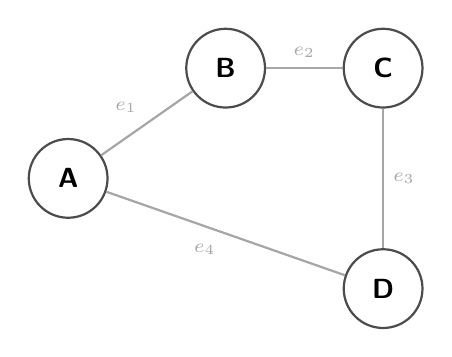
\begin{tikzpicture}[
    pnode/.style={circle, draw=black!70, fill=white, thick,
                  minimum size=1.0cm, font=\bfseries\sffamily},
    sedge/.style={thick, gray!70}
]
    \node[pnode] (A) at (0,0)   {A};
    \node[pnode] (B) at (2,1.4) {B};
    \node[pnode] (C) at (4,1.4) {C};
    \node[pnode] (D) at (4,-1.4){D};

    \draw[sedge] (A) -- node[above left,  font=\scriptsize]{$e_1$} (B);
    \draw[sedge] (B) -- node[above,       font=\scriptsize]{$e_2$} (C);
    \draw[sedge] (C) -- node[right,       font=\scriptsize]{$e_3$} (D);
    \draw[sedge] (A) -- node[below left,  font=\scriptsize]{$e_4$} (D);
\end{tikzpicture}
\caption{The \textbf{static projection} of the four contacts. All edges exist
simultaneously. A graph algorithm sees $A$--$B$--$C$--$D$ and also
$A$--$D$--$C$--$B$, $A$--$D$--$C$--$B$, and so on.}
\label{fig:static_projection}
\end{figure}

On this static graph, every simple path between every pair of nodes is
available. A naive GNN that operates on this graph would conclude, for example,
that the path $D \to C \to B \to A$ is a valid transmission route (Dave infects
Carol, Carol infects Bob, Bob infects Alice). But this is \textbf{physically
impossible}:

\begin{itemize}
    \item Dave only met Carol at $t=3$.
    \item Carol had already met Bob at $t=2$ --- \emph{one time step earlier}.
    \item A pathogen cannot travel backwards in time: Dave cannot have infected
          Carol at $t=3$ and then Carol retroactively infects Bob at $t=2$.
\end{itemize}

\begin{keyinsight}{Static Graphs Create Phantom Paths}
The static projection introduces \textbf{phantom paths} --- paths that look
valid topologically but are causally impossible because the timestamps are
in the wrong order. Any GNN that ignores event timing will learn from these
phantom paths and will be systematically mis-calibrated about the true source.
The core challenge of this entire chapter, and of the Saram\"{a}ki paper, is
to build a data structure that makes it \emph{structurally impossible} to
traverse a phantom path.
\end{keyinsight}

% =============================================================================
\section{The Saram\"{a}ki Insight: Make Events the Nodes}
\label{sec:saramaki_insight}
% =============================================================================

The elegant solution proposed by Saram\"{a}ki, Kivel\"{a}, and Karsai in their
2019 paper ``Weighted temporal event graphs'' \cite{saramaki2019temporal} is a
\textbf{perspective shift} so simple it is almost surprising that it works so
well.

\begin{keyinsight}{The Central Idea: Elevate Events to Nodes}
Instead of treating \emph{people} as graph nodes and \emph{contacts} as edges,
we \textbf{swap the roles}:
\begin{itemize}[noitemsep]
    \item \textbf{People} disappear as primary nodes.
    \item \textbf{Contact events} $(u, v, t)$ become the new nodes of a graph.
    \item \textbf{Causal relationships between events} become directed edges.
\end{itemize}
The result is a new graph --- the \textbf{Temporal Event Graph (TEG)} --- where
the very structure of the graph encodes temporal causality. You cannot traverse
a phantom path because phantom edges simply do not exist in the TEG.
\end{keyinsight}

\subsection{Why This Solves the Problem}

On the original temporal network, phantom paths arise because a GNN cannot
distinguish the \emph{order} of edges incident on a node. Person $B$ is
connected to both $A$ and $C$ in the static graph, and nothing in the adjacency
matrix tells you that $B$ met $A$ first.

In the Temporal Event Graph, the two events ``$B$ meets $A$'' and ``$B$ meets
$C$'' are \emph{separate nodes}. A directed edge from event $e_1=(A,B,t{=}1)$
to event $e_2=(B,C,t{=}2)$ means ``$e_1$ can causally enable $e_2$'' --- which
is precisely true: $B$ was infected at $t=1$ and can pass the virus on at
$t=2$. The reverse edge $e_2 \to e_1$ does not exist, making the phantom path
structurally absent.

\begin{analogybox}{The Train Timetable vs. the Railway Map}
A standard railway map shows you which cities are connected by rail. You might
conclude that you can travel from London to Edinburgh in any order. The
\emph{timetable}, however, makes an explicit graph of which trains you can
catch after getting off another train. If Train A arrives at Birmingham at
12:00 and Train B departs Birmingham at 11:30, there is no edge from Train A
to Train B in the timetable graph --- the connection is physically impossible.
The Temporal Event Graph is the timetable. The static projection is the map.
\end{analogybox}

\subsection{Our Four Events as Nodes}

Let us apply this idea to the Alice/Bob/Carol/Dave example. We have four
events. In the TEG, these become four nodes:

\begin{center}
\begin{tabular}{ccccc}
\toprule
\textbf{TEG Node} & \textbf{Original Event} & \textbf{People} & \textbf{Time} \\
\midrule
$v_{e_1}$ & $e_1$ & Alice, Bob   & $t=1$ \\
$v_{e_2}$ & $e_2$ & Bob, Carol   & $t=2$ \\
$v_{e_3}$ & $e_3$ & Carol, Dave  & $t=3$ \\
$v_{e_4}$ & $e_4$ & Alice, Dave  & $t=4$ \\
\bottomrule
\end{tabular}
\end{center}

The question ``which event can causally follow which?'' is now the question
``which directed edges exist between these four TEG nodes?'' We answer this
systematically in the next section.

% =============================================================================
\section{Formal Construction of the Temporal Event Graph}
\label{sec:teg_construction}
% =============================================================================

\begin{mathbox}{Definition: Temporal Event Graph (TEG)}
Let $G^T = (V, E^T)$ be a temporal network with event set
$E^T = \{e_1, e_2, \dots, e_m\}$ where each event $e_i = (u_i, v_i, t_i)$.

We construct the \textbf{Temporal Event Graph} $D = (V_D, E_D, W)$ as follows:

\medskip
\noindent\textbf{Nodes:}
\[
    V_D = \{ v_{e_i} \mid e_i \in E^T \}
\]
Each original event $e_i$ becomes exactly one node $v_{e_i}$ in $D$. So
$|V_D| = |E^T|$.

\medskip
\noindent\textbf{Directed Edges:}
\[
    E_D = \{ (v_{e_i}, v_{e_j}) \mid \text{nodes}(e_i) \cap \text{nodes}(e_j)
    \neq \emptyset \; \wedge \; t_j > t_i \; \wedge \; t_j - t_i \le \Delta t \}
\]
where $\text{nodes}(e_i) = \{u_i, v_i\}$ is the pair of people in event $e_i$,
and $\Delta t \in \mathbb{R}^+ \cup \{\infty\}$ is an optional \textbf{time
window} (the unconstrained TEG uses $\Delta t = \infty$).

In words, a directed edge $e_i \to e_j$ exists if and only if:
\begin{enumerate}[noitemsep]
    \item \textbf{Shared person:} $e_i$ and $e_j$ involve at least one common
          person. This is the individual who \emph{carries} the pathogen between
          the two events.
    \item \textbf{Strict chronological order:} $t_j > t_i$. The second event
          must happen \emph{after} the first. Strictly greater than, not
          equal to.
    \item \textbf{Infectious window (optional):} $t_j - t_i \le \Delta t$. The
          gap between the two events must not exceed the maximum infectious
          period. If a person holds the pathogen for longer than $\Delta t$ time
          units, they are assumed to have recovered and cannot transmit.
\end{enumerate}

\medskip
\noindent\textbf{Edge Weights:}
\[
    w_{ij} = t_j - t_i
\]
The weight of edge $e_i \to e_j$ is the \textbf{inter-event time} $\tau_{ij}$:
how long the shared person waited between receiving the pathogen (at $e_i$) and
potentially passing it on (at $e_j$).
\end{mathbox}

\subsection{Why This Graph is Always a DAG}

The condition $t_j > t_i$ (strictly greater) is the key to a crucial structural
guarantee.

\begin{conceptbox}{The TEG is a Directed Acyclic Graph (DAG)}
\textbf{Claim:} $D = (V_D, E_D)$ contains no directed cycles.

\medskip
\noindent\textbf{Proof sketch:} Suppose for contradiction that there is a
directed cycle: $e_{i_1} \to e_{i_2} \to \cdots \to e_{i_k} \to e_{i_1}$.
Each directed edge in this cycle requires that the timestamp of the destination
is strictly greater than the timestamp of the source. Chaining these inequalities:
\[
    t_{i_1} < t_{i_2} < \cdots < t_{i_k} < t_{i_1}
\]
This gives $t_{i_1} < t_{i_1}$, a contradiction. Therefore no cycle can
exist. $\square$

\medskip
The consequence is profound: the TEG has a guaranteed \textbf{topological
ordering} aligned with real time. Information can flow in only one direction
--- from the past to the future. This makes the TEG perfectly suited for
message-passing algorithms that need to respect the arrow of time.
\end{conceptbox}

\subsection{Explaining Each Condition with Concrete Examples}

Let us verify each condition using the Alice/Bob/Carol/Dave events.

\paragraph{Condition 1: Shared person.}
Event $e_1=(A,B,t=1)$ and event $e_2=(B,C,t=2)$ share the person \textbf{Bob}.
So Condition 1 is satisfied and there \emph{may} be an edge. By contrast,
$e_1=(A,B,t=1)$ and $e_3=(C,D,t=3)$ share \emph{no person}; there is no
individual who could carry the pathogen between these two events directly.
Condition 1 fails, so no edge exists regardless of timing.

\paragraph{Condition 2: Strict chronological order.}
Consider $e_2=(B,C,t=2)$ and $e_1=(A,B,t=1)$. They share Bob. But $t_1 = 1 <
t_2 = 2$, so the direction would be $e_1 \to e_2$, not $e_2 \to e_1$. An edge
$e_2 \to e_1$ would require $t_1 > t_2$, which is false. So there is an edge
from $e_1$ to $e_2$ but \emph{not} from $e_2$ to $e_1$.

\paragraph{Condition 3: Infectious window.}
Consider $e_1=(A,B,t=1)$ and $e_3=(C,D,t=3)$. These share no person, so there
is already no edge. But suppose we had an event $e_1'=(A,B,t=1)$ and
$e_2'=(B,C,t=10)$ in some other scenario. They share Bob, and $t=10 > t=1$.
With $\Delta t = 7$ days: $10 - 1 = 9 > 7$, so no edge exists (Bob recovered
before meeting Carol). With $\Delta t = \infty$: an edge exists. The $\Delta t$
parameter acts as a biological pruning criterion.

% =============================================================================
\section{Full Worked Example: Building the TEG Step by Step}
\label{sec:teg_worked}
% =============================================================================

We now systematically build the TEG for the four-event scenario. The method is
straightforward: consider every ordered pair of events $(e_i, e_j)$ with
$i \neq j$, and check the three conditions.

\subsection{Checking All Ordered Pairs}

We use $\Delta t = \infty$ (unconstrained) for this first pass.

\begin{examplebox}{Exhaustive Edge Check for $\Delta t = \infty$}
\small
\begin{center}
\begin{tabular}{ccccccc}
\toprule
\textbf{Pair} & $e_i$ & $e_j$ & \textbf{Shared person?} & $t_j > t_i$? & $t_j - t_i$ & \textbf{Edge?} \\
\midrule
$(e_1, e_2)$ & $(A,B,1)$ & $(B,C,2)$ & Yes (B) & $2>1$: Yes & 1 & \textbf{Yes: $e_1 \to e_2$} \\
$(e_1, e_3)$ & $(A,B,1)$ & $(C,D,3)$ & No      & ---        & --- & No \\
$(e_1, e_4)$ & $(A,B,1)$ & $(A,D,4)$ & Yes (A) & $4>1$: Yes & 3 & \textbf{Yes: $e_1 \to e_4$} \\
$(e_2, e_1)$ & $(B,C,2)$ & $(A,B,1)$ & Yes (B) & $1>2$: No  & --- & No \\
$(e_2, e_3)$ & $(B,C,2)$ & $(C,D,3)$ & Yes (C) & $3>2$: Yes & 1 & \textbf{Yes: $e_2 \to e_3$} \\
$(e_2, e_4)$ & $(B,C,2)$ & $(A,D,4)$ & No      & ---        & --- & No \\
$(e_3, e_1)$ & $(C,D,3)$ & $(A,B,1)$ & No      & $1>3$: No  & --- & No \\
$(e_3, e_2)$ & $(C,D,3)$ & $(B,C,2)$ & Yes (C) & $2>3$: No  & --- & No \\
$(e_3, e_4)$ & $(C,D,3)$ & $(A,D,4)$ & Yes (D) & $4>3$: Yes & 1 & \textbf{Yes: $e_3 \to e_4$} \\
$(e_4, e_1)$ & $(A,D,4)$ & $(A,B,1)$ & Yes (A) & $1>4$: No  & --- & No \\
$(e_4, e_2)$ & $(A,D,4)$ & $(B,C,2)$ & No      & $2>4$: No  & --- & No \\
$(e_4, e_3)$ & $(A,D,4)$ & $(C,D,3)$ & Yes (D) & $3>4$: No  & --- & No \\
\bottomrule
\end{tabular}
\end{center}

\medskip
\noindent\textbf{Result:} The TEG has exactly four edges:
\[
    E_D = \{ e_1 \to e_2,\; e_1 \to e_4,\; e_2 \to e_3,\; e_3 \to e_4 \}
\]
with weights $w_{12}=1$, $w_{14}=3$, $w_{23}=1$, $w_{34}=1$.
\end{examplebox}

\subsection{The Resulting TEG: A TikZ Diagram}

\begin{figure}[H]
\centering
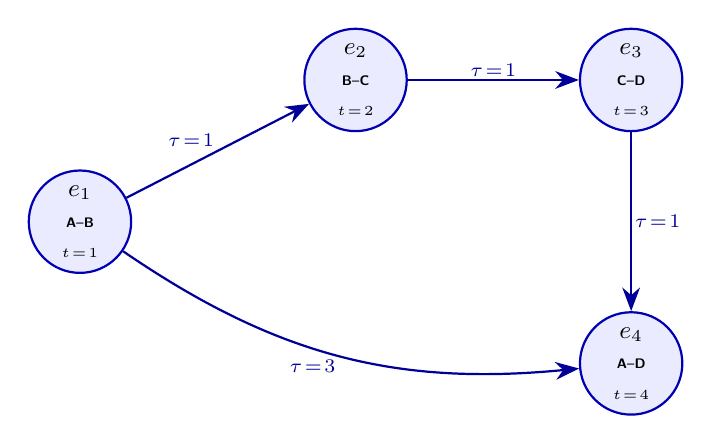
\begin{tikzpicture}[
    eventnode/.style={
        circle, draw=blue!70!black, fill=blue!8!white, thick,
        minimum size=1.3cm, font=\small\bfseries\sffamily, align=center,
        inner sep=2pt
    },
    arr/.style={-{Stealth[length=3mm]}, thick, blue!60!black},
    wlabel/.style={font=\scriptsize\sffamily, fill=white, inner sep=1pt}
]
    % Nodes: laid out left-to-right by time
    \node[eventnode] (e1) at (0, 0)    {$e_1$\\{\tiny A--B}\\{\tiny $t\!=\!1$}};
    \node[eventnode] (e2) at (3.5, 1.8){$e_2$\\{\tiny B--C}\\{\tiny $t\!=\!2$}};
    \node[eventnode] (e3) at (7.0, 1.8){$e_3$\\{\tiny C--D}\\{\tiny $t\!=\!3$}};
    \node[eventnode] (e4) at (7.0,-1.8){$e_4$\\{\tiny A--D}\\{\tiny $t\!=\!4$}};

    % Edges
    \draw[arr] (e1) -- node[wlabel, above left]{$\tau\!=\!1$} (e2);
    \draw[arr] (e1) to[bend right=20] node[wlabel, below left]{$\tau\!=\!3$} (e4);
    \draw[arr] (e2) -- node[wlabel, above]{$\tau\!=\!1$} (e3);
    \draw[arr] (e3) -- node[wlabel, right]{$\tau\!=\!1$} (e4);
\end{tikzpicture}
\caption{The \textbf{Temporal Event Graph (TEG)} for the four-event scenario,
with $\Delta t = \infty$. Nodes are contact events; directed edges represent
valid causal pathways. Edge weights $\tau = t_j - t_i$ are the inter-event
waiting times. The graph flows strictly left-to-right (past to future) and
contains no cycles.}
\label{fig:teg_full}
\end{figure}

\subsection{Reading the TEG}

Let us read the causal structure directly from Figure~\ref{fig:teg_full}:

\begin{itemize}
    \item \textbf{$e_1 \to e_2$:} Bob was in event $e_1$ (with Alice) and then
          in event $e_2$ (with Carol). Bob could carry the virus from $e_1$ to
          $e_2$. Inter-event time: 1 time unit.
    \item \textbf{$e_2 \to e_3$:} Carol was in $e_2$ and then in $e_3$. Carol
          could carry the virus. Inter-event time: 1 time unit.
    \item \textbf{$e_3 \to e_4$:} Dave was in $e_3$ and then in $e_4$. Dave
          could carry the virus onward. Inter-event time: 1 time unit.
    \item \textbf{$e_1 \to e_4$:} Alice was in $e_1$ and then in $e_4$. Alice
          could also carry the virus from $e_1$ directly to $e_4$, skipping the
          chain via Bob and Carol. Inter-event time: 3 time units.
\end{itemize}

The path $A \to B \to C \to D$ is represented in the TEG as the directed path
$e_1 \to e_2 \to e_3 \to e_4$. The phantom path $D \to C \to B \to A$ has no
corresponding path in the TEG because no edges point backwards in time.

% =============================================================================
\section{The $\Delta t$ Constraint: Modelling the Infectious Period}
\label{sec:teg_delta_t}
% =============================================================================

The unconstrained TEG ($\Delta t = \infty$) encodes all \emph{topologically
possible} causal chains under the sole constraint of strict temporal ordering.
But biology imposes an additional restriction: an infected person eventually
recovers and can no longer transmit the pathogen. This is modelled by the
$\Delta t$ parameter.

\begin{conceptbox}{Biological Meaning of $\Delta t$}
$\Delta t$ is the \textbf{maximum infectious period}. If a shared person
participates in event $e_i$ at time $t_i$ and event $e_j$ at time $t_j$, with
$t_j - t_i > \Delta t$, then by the time $e_j$ occurs the person has already
recovered. They cannot carry the pathogen from $e_i$ to $e_j$.

In the SIR model, $\Delta t$ corresponds roughly to $1/\mu$ (the reciprocal
of the recovery rate). In practice, $\Delta t$ is a hyperparameter that
controls how aggressively we prune the TEG.
\end{conceptbox}

\subsection{Recomputing with $\Delta t = 1$}

Apply $\Delta t = 1$ to our four-event example. For each candidate edge, we
check whether $t_j - t_i \le 1$:

\begin{examplebox}{Edge Check with $\Delta t = 1$}
\begin{center}
\begin{tabular}{ccccc}
\toprule
\textbf{Candidate Edge} & $t_j - t_i$ & $\le \Delta t = 1$? & \textbf{Edge survives?} \\
\midrule
$e_1 \to e_2$ & $2-1=1$ & Yes & \textbf{Yes} \\
$e_1 \to e_4$ & $4-1=3$ & No  & \textbf{Pruned} \\
$e_2 \to e_3$ & $3-2=1$ & Yes & \textbf{Yes} \\
$e_3 \to e_4$ & $4-3=1$ & Yes & \textbf{Yes} \\
\bottomrule
\end{tabular}
\end{center}

\medskip
With $\Delta t = 1$, the edge $e_1 \to e_4$ is removed. Alice cannot carry
the virus from her meeting with Bob ($t=1$) all the way to her meeting with
Dave ($t=4$), because she would have recovered by then.

The pruned TEG has three edges: $\{e_1 \to e_2,\; e_2 \to e_3,\; e_3 \to
e_4\}$, forming a simple directed path.
\end{examplebox}

\begin{figure}[H]
\centering
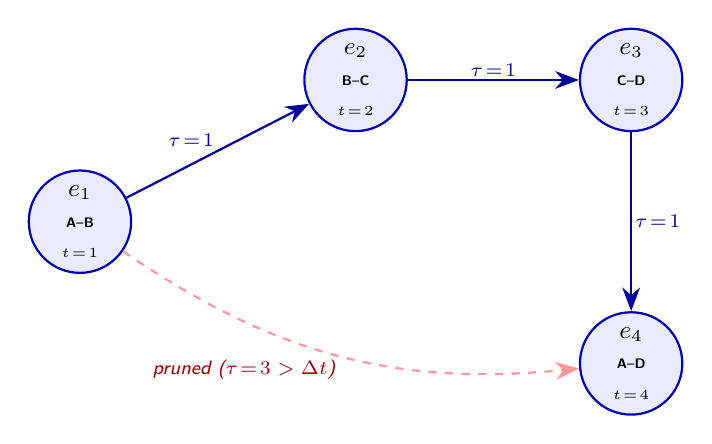
\begin{tikzpicture}[
    eventnode/.style={
        circle, draw=blue!70!black, fill=blue!8!white, thick,
        minimum size=1.3cm, font=\small\bfseries\sffamily, align=center,
        inner sep=2pt
    },
    eventdead/.style={
        circle, draw=gray!50, fill=gray!8!white, thick, dashed,
        minimum size=1.3cm, font=\small\bfseries\sffamily, align=center,
        inner sep=2pt
    },
    arr/.style={-{Stealth[length=3mm]}, thick, blue!60!black},
    arrpruned/.style={-{Stealth[length=3mm]}, thick, red!40!white, dashed},
    wlabel/.style={font=\scriptsize\sffamily, fill=white, inner sep=1pt}
]
    \node[eventnode] (e1) at (0, 0)    {$e_1$\\{\tiny A--B}\\{\tiny $t\!=\!1$}};
    \node[eventnode] (e2) at (3.5, 1.8){$e_2$\\{\tiny B--C}\\{\tiny $t\!=\!2$}};
    \node[eventnode] (e3) at (7.0, 1.8){$e_3$\\{\tiny C--D}\\{\tiny $t\!=\!3$}};
    \node[eventnode] (e4) at (7.0,-1.8){$e_4$\\{\tiny A--D}\\{\tiny $t\!=\!4$}};

    % Surviving edges
    \draw[arr] (e1) -- node[wlabel, above left]{$\tau\!=\!1$} (e2);
    \draw[arr] (e2) -- node[wlabel, above]{$\tau\!=\!1$} (e3);
    \draw[arr] (e3) -- node[wlabel, right]{$\tau\!=\!1$} (e4);

    % Pruned edge
    \draw[arrpruned] (e1) to[bend right=20]
        node[font=\scriptsize\sffamily\itshape, color=red!60!black, fill=white,
             inner sep=1pt, below left]{pruned ($\tau\!=\!3 > \Delta t$)} (e4);
\end{tikzpicture}
\caption{TEG with $\Delta t = 1$. The long-range edge $e_1 \to e_4$ (dashed
red) is pruned because the inter-event time $\tau = 3$ exceeds the infectious
window $\Delta t = 1$. Only the tight causal chain $e_1 \to e_2 \to e_3 \to
e_4$ survives.}
\label{fig:teg_pruned}
\end{figure}

\subsection{The Effect of $\Delta t$ on Graph Density}

\begin{keyinsight}{$\Delta t$ Controls the Sparsity--Completeness Trade-off}
\begin{itemize}[noitemsep]
    \item A \textbf{large} $\Delta t$ (close to $\infty$) retains all causal
          chains but produces a denser TEG, potentially with $O(E^2)$ edges.
    \item A \textbf{small} $\Delta t$ prunes many edges, producing a sparser
          TEG that is faster to process but may discard valid long-range causal
          paths.
    \item In practice, $\Delta t$ should be chosen to match the \emph{mean
          infectious period} of the disease being modelled. For the SIR model
          with recovery rate $\mu$, a natural choice is $\Delta t \approx 1/\mu$.
\end{itemize}
\end{keyinsight}

% =============================================================================
\section{Why a DAG is Perfect for Source Detection with GNNs}
\label{sec:teg_dag_gnn}
% =============================================================================

We now have a clean DAG encoding all causal paths in the temporal network. Why
is this particularly useful for \emph{source detection}?

\subsection{The Source Detection Problem on the TEG}

Recall the source detection problem: we observe the final infection state of
the network --- who is Susceptible (S), Infected (I), or Recovered (R) at time
$T$ --- and we must identify which node started the outbreak.

In the TEG, the source node is the person who was involved in the
\textbf{earliest events} of the causal chain. Evidence about the source is
therefore concentrated in the \emph{early event nodes} of the TEG.

\begin{conceptbox}{Source Detection as a Backward Flow Problem}
The TEG has a natural ``direction of causality'': edges point from earlier
events to later events (past $\to$ future). The epidemic spreads \emph{forward}
through this DAG: the source's first contact enables later contacts, which
enable even later ones.

To \emph{detect} the source, we must work \emph{backwards}: starting from the
observable outcome (who is recovered at time $T$), we must propagate evidence
back through the causal chain to identify the likely origin.

This suggests a GNN that operates on the \textbf{reversed DAG}: flip every
edge direction so that information flows from late events (observed outcomes)
toward early events (causal predecessors). After several rounds of message
passing on the reversed DAG, the earliest event nodes will have aggregated
evidence from all downstream events they enabled, making them the most
``informed'' nodes --- and most likely to correspond to the source.
\end{conceptbox}

\subsection{Visualising the Reversed DAG}

\begin{figure}[H]
\centering
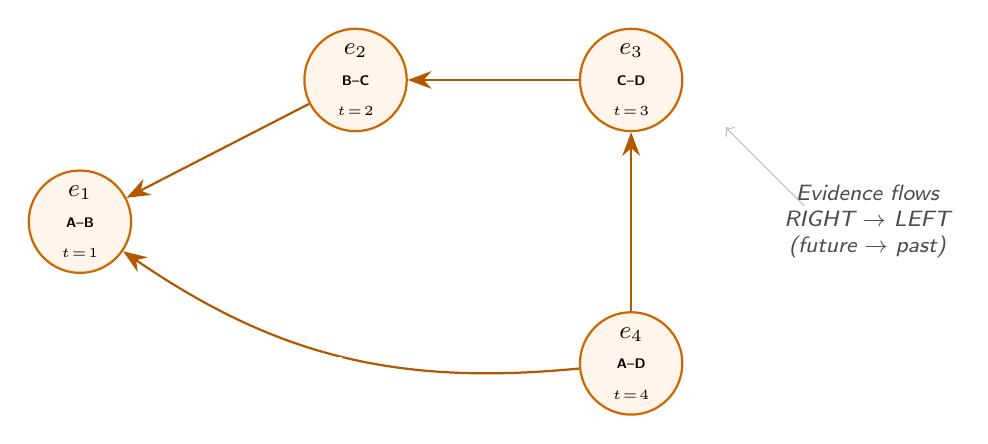
\begin{tikzpicture}[
    eventnode/.style={
        circle, draw=orange!80!black, fill=orange!8!white, thick,
        minimum size=1.3cm, font=\small\bfseries\sffamily, align=center,
        inner sep=2pt
    },
    arr/.style={-{Stealth[length=3mm]}, thick, orange!70!black},
    wlabel/.style={font=\scriptsize\sffamily, fill=white, inner sep=1pt},
    infolabel/.style={font=\footnotesize\sffamily\itshape, text=gray!60!black}
]
    \node[eventnode] (e1) at (0, 0)    {$e_1$\\{\tiny A--B}\\{\tiny $t\!=\!1$}};
    \node[eventnode] (e2) at (3.5, 1.8){$e_2$\\{\tiny B--C}\\{\tiny $t\!=\!2$}};
    \node[eventnode] (e3) at (7.0, 1.8){$e_3$\\{\tiny C--D}\\{\tiny $t\!=\!3$}};
    \node[eventnode] (e4) at (7.0,-1.8){$e_4$\\{\tiny A--D}\\{\tiny $t\!=\!4$}};

    % Reversed edges: arrows point BACKWARD in time
    \draw[arr] (e2) -- node[wlabel, above left]{} (e1);
    \draw[arr] (e3) -- node[wlabel, above]{}      (e2);
    \draw[arr] (e4) -- node[wlabel, right]{}      (e3);
    \draw[arr] (e4) to[bend left=20]
        node[wlabel, below]{}                     (e1);

    % Annotation arrows
    \node[infolabel, align=center] at (10.0, 0)
        {Evidence flows\\RIGHT $\to$ LEFT\\(future $\to$ past)};
    \draw[->, gray!50, thin] (9.2, 0.2) -- (8.2, 1.2);
\end{tikzpicture}
\caption{The \textbf{reversed TEG} (using $\Delta t = \infty$ version). Every
arrow has been flipped. Information about who is Recovered now flows from late
events ($e_4, e_3$) backward toward early events ($e_1$). After message
passing, early event $e_1$ accumulates evidence from the entire chain.}
\label{fig:teg_reversed}
\end{figure}

\subsection{From Event Scores Back to Person Scores}

After running a GNN on the reversed DAG, each event node $v_{e_i}$ has a
learned embedding. To produce a final ranking of \emph{people} (which person
is the source?), we aggregate the event embeddings back to the person level.
Each person's score is the sum (or mean) of the embeddings of all events they
participated in. If Alice (the true source) participated in $e_1$ (an early
event with high aggregated evidence) and $e_4$ (a late event), her summed score
will be higher than Dave's, who only participated in $e_3$ and $e_4$.

% =============================================================================
\section{Code Walkthrough: The \texttt{DAGGNN} Architecture}
\label{sec:dag_gnn_code}
% =============================================================================

The ideas developed above are implemented in
\texttt{gnn/dag\_gnn.py}. We now walk through the code step by step, connecting
each piece to the mathematical concepts above. The file contains two classes:
\texttt{DAGConvLayer} (a single message-passing layer) and \texttt{DAGGNN} (the
complete model).

\begin{conceptbox}{Model Inputs and Outputs}
The \texttt{DAGGNN.forward} method receives four arguments:
\begin{itemize}[noitemsep]
    \item \texttt{x}: shape \texttt{[B, N, 3]} --- the observed SIR state of
          every person, encoded as a one-hot vector \texttt{[1,0,0]} (S),
          \texttt{[0,1,0]} (I), or \texttt{[0,0,1]} (R). $B$ is the batch size
          and $N$ is the number of people.
    \item \texttt{dag\_edge\_index}: shape \texttt{[2, E\_dag]} --- the
          \emph{forward} causal edges of the TEG (before reversal). Each column
          $[\,i,\,j\,]^\top$ means event $i$ causally precedes event $j$.
    \item \texttt{event\_to\_node}: shape \texttt{[n\_events]} --- for each
          event, the index of the ``arriving'' person (the one receiving the
          potential transmission).
    \item \texttt{event\_src\_node}: shape \texttt{[n\_events]} --- for each
          event, the index of the ``departing'' person (the one possibly
          transmitting).
\end{itemize}
The output is a log-softmax distribution over all $N$ people: the model's
belief about who is the epidemic source.
\end{conceptbox}

\begin{codewalk}{Step 1 --- Event Feature Construction}
The first challenge: the TEG nodes are \emph{events}, but our input data
\texttt{x} contains features for \emph{people}. We must construct an initial
feature vector for each event from the health states of the two people involved.

\medskip
Each person's SIR state is a 3-dimensional one-hot vector:
\[
\text{Susceptible} \to [1,0,0], \quad
\text{Infected} \to [0,1,0], \quad
\text{Recovered} \to [0,0,1]
\]
For event $e_k = (u, v, t_k)$, we look up person $u$'s state $\mathbf{x}_u \in
\mathbb{R}^3$ and person $v$'s state $\mathbf{x}_v \in \mathbb{R}^3$, then
concatenate them into a 6-dimensional vector:
\[
    \mathbf{f}_{e_k} = [\mathbf{x}_u \;\|\; \mathbf{x}_v] \in \mathbb{R}^6
\]
This is then projected into the hidden dimension $D$ via a learned linear layer
with ReLU activation:
\[
    \mathbf{h}_{e_k}^{(0)} = \text{ReLU}\!\left( \mathbf{W}_{\text{proj}} \,
    \mathbf{f}_{e_k} + \mathbf{b}_{\text{proj}} \right) \in \mathbb{R}^D
\]

\begin{lstlisting}[language=Python]
# ev_src: [n_events] — index of "source" person in each event
# ev_dst: [n_events] — index of "destination" person in each event
ev_src = event_src_node.to(x.device)   # [n_events]
ev_dst = event_to_node.to(x.device)    # [n_events]

# Index into x to get person features: [B, n_events, 3]
x_src = x[:, ev_src, :]
x_dst = x[:, ev_dst, :]

# Concatenate along feature dimension: [B, n_events, 6]
# Project to hidden dim D via self.proj_event (Linear(6, D)): [B, n_events, D]
h = F.relu(self.proj_event(torch.cat([x_src, x_dst], dim=-1)))
\end{lstlisting}

\textbf{Numerical example.}
Suppose event $e_1 = (\text{Alice, Bob})$ and at observation time:
\begin{itemize}[noitemsep]
    \item Alice is Recovered: $\mathbf{x}_A = [0, 0, 1]$
    \item Bob is also Recovered: $\mathbf{x}_B = [0, 0, 1]$
\end{itemize}
The concatenated feature vector for $e_1$ is
$\mathbf{f}_{e_1} = [0,0,1,\;0,0,1] \in \mathbb{R}^6$.
This is then projected: $\mathbf{h}_{e_1}^{(0)} = \text{ReLU}(\mathbf{W} \cdot [0,0,1,0,0,1]^\top + \mathbf{b}) \in \mathbb{R}^D$.

The intuition is that an event in which \emph{both} participants ended up
Recovered is a strong candidate for a transmission event. An event in which one
person is Susceptible (they were never infected) is far less informative about
the source.
\end{codewalk}

\begin{codewalk}{Step 2 --- Reversing the Arrow of Time}
As established in Section~\ref{sec:teg_dag_gnn}, source detection requires
information to flow \emph{backward} through the causal chain. We reverse every
edge in the TEG by simply swapping the two rows of the edge index tensor.

In PyTorch Geometric convention, \texttt{edge\_index} is a $2 \times E$ tensor
where row 0 contains source node indices and row 1 contains destination node
indices. Flipping row 0 and row 1 reverses every edge direction:

\begin{lstlisting}[language=Python]
# dag_edge_index: [2, E_dag], forward edges e_i -> e_j (t_i < t_j)
# After flip: row 0 becomes old row 1 (destinations become sources)
#             row 1 becomes old row 0 (sources become destinations)
# Effect: edge [e_i, e_j] becomes [e_j, e_i]  (backward in time)
if dag_edge_index.numel() > 0:
    rev_ei = dag_edge_index.flip(0).to(x.device)  # [2, E_dag]
else:
    rev_ei = dag_edge_index.to(x.device)
\end{lstlisting}

\textbf{Concrete example.}
Suppose \texttt{dag\_edge\_index} is:
\[
\begin{pmatrix} 0 & 1 & 2 \\ 1 & 2 & 3 \end{pmatrix}
\]
representing edges $e_0 \to e_1$, $e_1 \to e_2$, $e_2 \to e_3$ (a causal chain).
After \texttt{.flip(0)}:
\[
\begin{pmatrix} 1 & 2 & 3 \\ 0 & 1 & 2 \end{pmatrix}
\]
Now the edges are $e_1 \to e_0$, $e_2 \to e_1$, $e_3 \to e_2$: information
flows from event 3 (the latest) all the way back to event 0 (the earliest),
exactly as required.
\end{codewalk}

\begin{codewalk}{Step 3 --- \texttt{DAGConvLayer}: SAGE-Style Message Passing}
With the reversed edges in hand, we run $L$ rounds of message passing. Each
round is implemented by \texttt{DAGConvLayer}, which performs
\textbf{mean-aggregation} (GraphSAGE style):

\[
    \mathbf{h}_e^{(l+1)} = \text{ReLU}\!\left(
        \mathbf{W}_{\text{self}} \, \mathbf{h}_e^{(l)}
        \;+\; \mathbf{W}_{\text{agg}} \cdot
        \frac{1}{|\mathcal{N}_{\text{rev}}(e)|}
        \sum_{e' \in \mathcal{N}_{\text{rev}}(e)} \mathbf{h}_{e'}^{(l)}
    \right)
\]

where $\mathcal{N}_{\text{rev}}(e)$ is the set of events that send messages to
$e$ under the reversed edge set --- i.e., the events that $e$ \emph{causally
preceded} in the original TEG.

Let us trace through the implementation:

\begin{lstlisting}[language=Python]
def forward(self, h, rev_edge_index):
    # h: [B, n_events, D]
    # rev_edge_index: [2, E_dag]  — reversed (backward) causal edges
    B, n_events, D = h.shape
    E = rev_edge_index.shape[1]

    # --- Handle the edge case: graph with no edges ---
    if E == 0:
        return F.relu(self.W_self(h))  # no aggregation possible

    src, dst = rev_edge_index[0], rev_edge_index[1]

    # Step A: Gather features from the "sender" events
    # Under reversed edges, senders are the LATER events (original destinations)
    h_src = h[:, src, :]  # [B, E, D]

    # Step B: Scatter-add messages into the "receiver" events
    # Under reversed edges, receivers are the EARLIER events (original sources)
    dst_idx = dst.view(1, -1, 1).expand(B, E, D)
    agg_sum = h.new_zeros(B, n_events, D)
    agg_sum.scatter_add_(1, dst_idx, h_src)   # [B, n_events, D]

    # Step C: Mean normalisation — divide by in-degree (number of senders)
    deg = h.new_zeros(n_events)
    deg.scatter_add_(0, dst, torch.ones(E, device=h.device))
    deg = deg.clamp(min=1).view(1, n_events, 1)  # avoid division by zero
    agg_mean = agg_sum / deg                     # [B, n_events, D]

    # Step D: Combine self-embedding with aggregated neighbourhood embedding
    h_new = F.relu(self.W_self(h) + self.W_agg(agg_mean))
    return h_new
\end{lstlisting}

\textbf{Numerical example.}
Suppose $D = 2$, and event $e_1$ receives messages from $e_2$ and $e_3$ under
the reversed edges (meaning $e_1$ originally enabled both $e_2$ and $e_3$).
The current embeddings are:
\[
    \mathbf{h}_{e_2}^{(l)} = [0.5,\; 0.3], \quad
    \mathbf{h}_{e_3}^{(l)} = [0.2,\; 0.8]
\]

\textbf{Step A:} Gather: $h_{\text{src}} = \{[0.5, 0.3],\; [0.2, 0.8]\}$.

\textbf{Step B:} Scatter-add into $e_1$: sum = $[0.5+0.2,\; 0.3+0.8] = [0.7,\; 1.1]$.

\textbf{Step C:} Degree of $e_1$ is 2. Mean = $[0.7/2,\; 1.1/2] = [0.35,\; 0.55]$.

\textbf{Step D:} Let $\mathbf{h}_{e_1}^{(l)} = [0.4, 0.6]$, and let
$\mathbf{W}_{\text{self}} = \mathbf{W}_{\text{agg}} = \mathbf{I}$ (identity)
for simplicity. Then:
\[
    \mathbf{h}_{e_1}^{(l+1)} = \text{ReLU}([0.4, 0.6] + [0.35, 0.55])
    = \text{ReLU}([0.75, 1.15]) = [0.75, 1.15]
\]

After $L$ layers of this, event $e_1$ has integrated information from every
downstream event it causally enabled. If the epidemic truly originated with
Alice (who was in $e_1$), the embedding of $e_1$ will carry the highest
concentration of downstream evidence.
\end{codewalk}

\begin{codewalk}{Step 4 --- Readout: Mapping Event Embeddings Back to People}
After $L$ message-passing layers, we have an embedding $\mathbf{h}_{e_k}^{(L)}
\in \mathbb{R}^D$ for every event node. But the task asks for a probability
distribution over \emph{people}: who is the source?

The readout step aggregates event embeddings back to person-level representations:

\begin{lstlisting}[language=Python]
# Initialise person embeddings to zero: [B, N, D]
node_emb = torch.zeros(B, N, D, device=x.device)

# ev_dst: [n_events] — which person is the "destination" of each event
# For each event e_k, add its embedding h[e_k] to person ev_dst[k]
dst_idx = ev_dst.view(1, -1, 1).expand(B, n_events, D)
node_emb.scatter_add_(1, dst_idx, h)              # [B, N, D]

if self.agg == "mean":
    # Optionally normalise by the number of events each person participated in
    # (their temporal degree). Prevents high-degree nodes from dominating.
    count = torch.zeros(N, device=x.device)
    count.scatter_add_(0, ev_dst, torch.ones(n_events, device=x.device))
    count = count.clamp(min=1).view(1, N, 1)
    node_emb = node_emb / count

# Project to scalar score, mask impossible candidates, normalise to log-prob
scores = self.out(node_emb).squeeze(-1)           # [B, N]
susceptible_mask = x[..., 0].bool()               # S-nodes cannot be source
scores = scores.masked_fill(susceptible_mask, float("-inf"))
return F.log_softmax(scores, dim=-1)              # [B, N]
\end{lstlisting}

\textbf{Why does sum aggregation work?}
A node that was the epidemic source participated in \emph{many early events}
that each enabled long causal chains. Each of these early events has accumulated
rich downstream evidence through the backward message passing. Summing their
embeddings gives the source node a high cumulative score.

A node that was only involved in late events (as a recipient, not originator)
will have embeddings that contain only local information. Its sum score will be
lower.

\textbf{The susceptible mask.}
A node that is still Susceptible at observation time was \emph{never infected}.
It therefore cannot have been the source. We mask such nodes out with
$-\infty$ before the softmax, setting their probability to exactly zero.
\end{codewalk}

\subsection{Putting It All Together: The Full Forward Pass}

\begin{figure}[H]
\centering
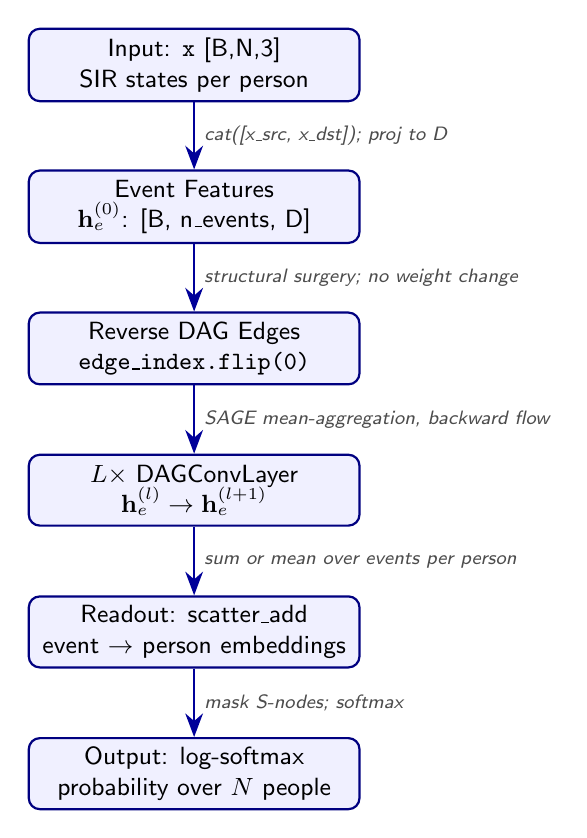
\begin{tikzpicture}[
    box/.style={rectangle, rounded corners=4pt, draw=blue!50!black,
                fill=blue!6!white, thick, minimum width=4.2cm,
                minimum height=0.9cm, font=\small\sffamily, align=center},
    arrow/.style={-{Stealth[length=3mm]}, thick, blue!60!black},
    label/.style={font=\scriptsize\sffamily\itshape, text=gray!60!black}
]
    \node[box] (inp)   at (0, 0)     {Input: \texttt{x} [B,N,3]\\SIR states per person};
    \node[box] (feat)  at (0,-1.8)   {Event Features\\$\mathbf{h}_e^{(0)}$: [B, n\_events, D]};
    \node[box] (rev)   at (0,-3.6)   {Reverse DAG Edges\\\texttt{edge\_index.flip(0)}};
    \node[box] (conv)  at (0,-5.4)   {$L \times$ DAGConvLayer\\$\mathbf{h}_e^{(l)} \to \mathbf{h}_e^{(l+1)}$};
    \node[box] (read)  at (0,-7.2)   {Readout: scatter\_add\\event $\to$ person embeddings};
    \node[box] (out)   at (0,-9.0)   {Output: log-softmax\\probability over $N$ people};

    \draw[arrow] (inp)  -- node[label, right]{cat([x\_src, x\_dst]); proj to D} (feat);
    \draw[arrow] (feat) -- node[label, right]{structural surgery; no weight change}    (rev);
    \draw[arrow] (rev)  -- node[label, right]{SAGE mean-aggregation, backward flow}   (conv);
    \draw[arrow] (conv) -- node[label, right]{sum or mean over events per person}      (read);
    \draw[arrow] (read) -- node[label, right]{mask S-nodes; softmax}                  (out);
\end{tikzpicture}
\caption{The complete \texttt{DAGGNN} forward pass. Data flows top to bottom:
people's health states are embedded as event features, the DAG is reversed,
message passing propagates evidence backward in time, and the readout maps
event evidence back to person scores.}
\label{fig:daggnn_pipeline}
\end{figure}

% =============================================================================
\section{The Graph Bloat Problem}
\label{sec:graph_bloat}
% =============================================================================

The TEG construction is mathematically elegant and computationally tractable
for small temporal networks. However, it has a significant scalability problem
that motivates the design choices in subsequent chapters.

\subsection{Worst-Case Edge Count}

\begin{mathbox}{TEG Edge Complexity}
Let $E = |E^T|$ be the number of contact events in the original temporal
network. In the unconstrained case ($\Delta t = \infty$), how many edges can
the TEG contain?

Consider $E$ events all involving the same person $v$, sorted by time
$t_1 < t_2 < \cdots < t_E$. Every pair $(e_i, e_j)$ with $i < j$ shares
person $v$ and satisfies $t_j > t_i$. So every such pair generates a directed
edge. The number of such pairs is:
\[
    \binom{E}{2} = \frac{E(E-1)}{2} = O(E^2)
\]
Thus the TEG can have \textbf{quadratically many edges} in the number of
contact events.
\end{mathbox}

\begin{examplebox}{Numerical Illustration of Graph Bloat}
Consider a network where a single ``super-spreader'' node participates in
$E = 100$ contact events over time. The TEG can then contain up to:
\[
    \frac{100 \times 99}{2} = 4{,}950 \text{ edges}
\]
just from this one person's event chain. If the network has $N$ nodes each with
$E/N$ events, the total TEG edges scale as $O(N \times (E/N)^2) = O(E^2/N)$.

For a realistic contact network with $E = 10{,}000$ events (a common size in
empirical datasets), the TEG could contain up to $\sim 50$ million edges. This
would make both memory storage and message-passing computationally prohibitive.
\end{examplebox}

\subsection{How $\Delta t$ Mitigates Bloat}

The $\Delta t$ constraint directly addresses graph bloat:

\begin{itemize}
    \item With $\Delta t = \infty$: an event $e_i$ at $t=1$ is connected to
          every later event $e_j$ at $t > 1$ involving a shared person.
    \item With $\Delta t = k$: event $e_i$ at $t=1$ is only connected to events
          $e_j$ in the window $t \in (1,\; 1+k]$.
\end{itemize}

If events are roughly uniformly distributed in time over an interval $[0, T]$,
then with $\Delta t$ constraint, each event has on average approximately
$\frac{\Delta t}{T} \cdot E$ causal successors instead of $E$. The edge count
drops from $O(E^2)$ to $O(E \cdot \frac{\Delta t}{T} \cdot E) = O(E^2 \cdot
\frac{\Delta t}{T})$, a multiplicative reduction of $\Delta t / T$.

\begin{keyinsight}{The $\Delta t$--Bloat Trade-off and the Need for Alternatives}
Graph bloat is not merely a computational nuisance. It points to a deeper
tension in the TEG approach:

\begin{itemize}[noitemsep]
    \item A \textbf{large} $\Delta t$ preserves all biologically plausible paths
          but creates a very dense TEG with many redundant edges.
    \item A \textbf{small} $\Delta t$ keeps the TEG sparse but may miss valid
          long-range causal chains.
    \item In the \textbf{worst case} (large $\Delta t$, many events on a single
          node), the TEG has $O(E^2)$ edges.
\end{itemize}

This motivates the architectures in Chapter~9 (Backtracking Network of Ru
et al.) and Chapter~10 (Qarkaxhija et al.), which operate on the original
contact graph rather than the TEG, embedding temporal information into edge
features and using different propagation strategies. Each approach trades
off causal exactness against computational feasibility.
\end{keyinsight}

% =============================================================================
\section{Summary: What the Saram\"{a}ki TEG Gives Us}
\label{sec:saramaki_summary}
% =============================================================================

We close this chapter with a structured comparison of what is gained and lost
by the TEG transformation.

\begin{center}
\begin{tabular}{lll}
\toprule
\textbf{Property} & \textbf{Static Graph} & \textbf{Temporal Event Graph} \\
\midrule
Preserves causal order & No & Yes \\
Phantom paths possible & Yes & No \\
Graph is a DAG & No & Always \\
Node semantics & People & Contact events \\
Edge semantics & ``ever met'' & ``can causally precede'' \\
Edge count & $O(N^2)$ & $O(E^2)$ worst case \\
GNN complexity & Standard MPNN & SAGE on reversed DAG \\
Scalability & High & Moderate (needs $\Delta t$ pruning) \\
\bottomrule
\end{tabular}
\end{center}

\medskip

The key takeaways from this chapter are:

\begin{enumerate}
    \item \textbf{Static graphs are wrong for causal reasoning.} They admit
          phantom paths that are physically impossible in a time-ordered system.
    \item \textbf{The TEG is a lossless transformation.} Every valid causal path
          in the temporal network corresponds to a directed path in the TEG, and
          vice versa. No information about feasible transmission chains is lost.
    \item \textbf{The TEG is always a DAG.} The strict $t_j > t_i$ requirement
          guarantees acyclicity, making standard GNN message passing well-defined
          and directional.
    \item \textbf{Source detection becomes backward inference.} By reversing the
          DAG, a GNN naturally aggregates evidence from observed outcomes toward
          early causal predecessors --- the likely source events.
    \item \textbf{Graph bloat is a real concern.} $O(E^2)$ edges in the worst
          case motivates the use of the $\Delta t$ constraint and alternative
          architectures.
\end{enumerate}

In the next chapter, we examine the Backtracking Network of Ru et al., which
takes a different approach: rather than lifting the problem to the event graph
level, it applies explicit probabilistic backtracking on the original temporal
network, using the SIR likelihood to guide message passing.

\chapter{The Backtracking Network: Temporal Information on Edges}

% =============================================================================
\section{The Core Idea: Two Philosophies of Temporal Encoding}
% =============================================================================

We have spent the previous chapter studying the Saram{\"a}ki framework, which solves the temporal-ordering problem by \textbf{rebuilding the graph from scratch}. Events become nodes in a Directed Acyclic Graph (DAG), and every node in that new graph now represents one single contact at one single moment in time. Causality is baked into the topology itself.

This is a powerful strategy. But it comes with a steep cost. Every temporal event $(u, v, t)$ in the original network becomes a node. Every causal adjacency between two events becomes an edge. In the worst case---a densely connected network where everyone meets everyone during a single infectious peak---the number of edges in the DAG can balloon to $O(E^2)$, where $E$ is the number of original contact events. This is the \textbf{Graph Bloat} problem.

The paper \textit{``Inferring Patient Zero on Temporal Networks via Graph Neural Networks''} by Ru, Lu, Wang, and Zeng (AAAI 2023) takes a fundamentally different path. Instead of rebuilding the graph structure, Ru et al.\ keep the original static graph---where nodes are people and edges are social ties---but equip every edge with a \textbf{memory of when it was active}. Temporal information is not encoded in topology; it is encoded in feature vectors that live on the edges.

\begin{conceptbox}{Two Philosophies Side by Side}
\begin{center}
\begin{tabular}{p{0.42\textwidth} p{0.42\textwidth}}
\toprule
\textbf{Saram{\"a}ki (DAG-GNN)} & \textbf{Ru et al.\ (Backtracking Network)} \\
\midrule
\textbf{Strategy:} Change the graph structure. Turn events into nodes. &
\textbf{Strategy:} Keep the original graph. Put temporal features on edges. \\[4pt]

\textbf{Graph size:} Grows with the number of events $E$. In the worst case, $O(E^2)$ edges in the DAG. &
\textbf{Graph size:} Identical to the original static graph. $|E|$ edges, each with a $T$-dimensional feature vector. Memory scales as $O(|E| \cdot T)$. \\[4pt]

\textbf{Temporal resolution:} Exact. Every event is a distinct entity. &
\textbf{Temporal resolution:} Binned. The continuous timeline is divided into $T$ discrete time slices. \\[4pt]

\textbf{Message passing:} Standard GNN on a new graph (events as nodes). &
\textbf{Message passing:} Novel edge-conditioned scheme: edges update first, then nodes. \\
\bottomrule
\end{tabular}
\end{center}
\end{conceptbox}

\begin{analogybox}{Two Maps of the Same City}
Imagine you are a detective trying to figure out where a rumour started in a city. You have records of every conversation that happened, with timestamps.

\textbf{The Saram{\"a}ki detective} builds an entirely new map. Instead of streets on the map, they plot each individual conversation as a location. They draw lines between conversations that could have passed the rumour. The result is a new, detailed map of causal flow---but it can be much larger than the original city map.

\textbf{The Ru et al.\ detective} keeps the original city map. But they attach a daily log to every street, recording which hours that street had traffic. The street between Alice's house and Bob's house now has a diary: ``Active on Monday at 9am, Wednesday at 3pm, Friday at noon.'' The detective can still reason about causality by reading these diaries---but without ever changing the map itself.

Both detectives can find the rumour's origin. They just carry different kinds of evidence.
\end{analogybox}

% =============================================================================
\section{Step 1: Representing the World in Numbers}
% =============================================================================

Before any neural network can run, every piece of information must be converted into a numerical tensor. The Backtracking Network requires two types of inputs: one for \textbf{nodes} (representing people and their health states) and one for \textbf{edges} (representing social contacts and when they occurred).

\subsection{Node Features: One-Hot SIR States}

At the end of an epidemic, we observe the health state of every person in the network. Each person is in exactly one of three states: Susceptible (S), Infectious (I), or Recovered (R).

We represent this as a \textbf{one-hot vector} of dimension 3:
\[
\text{Susceptible} \to \begin{bmatrix}1\\0\\0\end{bmatrix}, \quad
\text{Infectious} \to \begin{bmatrix}0\\1\\0\end{bmatrix}, \quad
\text{Recovered} \to \begin{bmatrix}0\\0\\1\end{bmatrix}
\]

\begin{keyinsight}{Why One-Hot and Not a Number 1, 2, 3?}
A natural question: why not encode S as 1, I as 2, R as 3? Numeric encoding implies an ordering and distance. It would tell the neural network that ``I is twice as much as S.'' But there is no such mathematical relationship among health states. One-hot encoding treats each state as a distinct, unordered category. The network learns relationships purely from data, not from an artificial numeric ordering.
\end{keyinsight}

Stacking the one-hot vectors for all $N$ people gives the \textbf{node feature matrix} $X \in \{0,1\}^{N \times 3}$.

\begin{examplebox}{Node Feature Matrix for 4 People}
Suppose at observation time:
\begin{itemize}[noitemsep]
    \item Person 0 (Alice): Susceptible
    \item Person 1 (Bob): Recovered
    \item Person 2 (Charlie): Recovered (the actual source)
    \item Person 3 (Diana): Infectious
\end{itemize}

\[
X = \begin{bmatrix}
1 & 0 & 0 \\
0 & 0 & 1 \\
0 & 0 & 1 \\
0 & 1 & 0
\end{bmatrix}
\quad
\begin{array}{l}
\leftarrow \text{Alice (S)} \\
\leftarrow \text{Bob (R)} \\
\leftarrow \text{Charlie (R) [true source]} \\
\leftarrow \text{Diana (I)}
\end{array}
\]

Notice that Alice (S) and Charlie (R, the source) have \textit{different} feature vectors. The source must be I or R---they had to be infected at some point. We will exploit this constraint later to eliminate impossible candidates.
\end{examplebox}

\subsection{Edge Features: Binary Activation Histories}

This is the key innovation of Ru et al. Every edge $(u, v)$ in the static graph gets a \textbf{binary vector of length $T$}, where $T$ is the number of time slices the observation window is divided into.

\begin{mathbox}{Edge Activation Vector Definition}
Let the observation window $[0, T_{\max}]$ be divided into $T$ equal time slices. For each edge $(u, v)$:
\[
a_{(u,v)} \in \{0, 1\}^T, \qquad a_{(u,v)}[t] = \begin{cases} 1 & \text{if $u$ and $v$ had contact in time slice $t$} \\ 0 & \text{otherwise} \end{cases}
\]
Collecting all edge activation vectors gives $A \in \{0,1\}^{|E| \times T}$.
\end{mathbox}

\begin{examplebox}{Edge Activation Vector: Alice and Bob ($T=10$)}
Alice (node 0) and Bob (node 1) had contact in hours 2, 5, and 8:

\begin{center}
\begin{tabular}{lccccccccccc}
\toprule
Time step $t$ & 0 & 1 & \textbf{2} & 3 & 4 & \textbf{5} & 6 & 7 & \textbf{8} & 9 \\
\midrule
Did they meet? & No & No & \textbf{Yes} & No & No & \textbf{Yes} & No & No & \textbf{Yes} & No \\
$a_{(0,1)}[t]$ & 0 & 0 & \textbf{1} & 0 & 0 & \textbf{1} & 0 & 0 & \textbf{1} & 0 \\
\bottomrule
\end{tabular}
\end{center}

\[
a_{(0,1)} = [\,0,\; 0,\; \mathbf{1},\; 0,\; 0,\; \mathbf{1},\; 0,\; 0,\; \mathbf{1},\; 0\,]
\]

If a virus entered Alice at time $t=1$, she \textit{could} have passed it to Bob at $t=2$ (the first $1$). If Alice was only infected at $t=6$, the earliest transmission to Bob would be at $t=8$. The timing of the $1$s determines which transmissions are causally possible.
\end{examplebox}

\begin{examplebox}{Full Edge Feature Matrix ($T=10$, 4 nodes, 5 edges)}
\[
A = \begin{blockarray}{cccccccccccl}
 & t_0 & t_1 & t_2 & t_3 & t_4 & t_5 & t_6 & t_7 & t_8 & t_9 & \\
\begin{block}{c[cccccccccc]l}
(0,1) & 0 & 0 & 1 & 0 & 0 & 1 & 0 & 0 & 1 & 0 & \leftarrow\text{Alice--Bob} \\
(0,2) & 0 & 1 & 0 & 1 & 0 & 0 & 0 & 0 & 0 & 0 & \leftarrow\text{Alice--Charlie} \\
(1,2) & 1 & 0 & 0 & 0 & 1 & 0 & 0 & 1 & 0 & 0 & \leftarrow\text{Bob--Charlie} \\
(1,3) & 0 & 0 & 0 & 0 & 0 & 0 & 1 & 0 & 0 & 1 & \leftarrow\text{Bob--Diana} \\
(2,3) & 0 & 0 & 0 & 1 & 0 & 0 & 0 & 1 & 0 & 0 & \leftarrow\text{Charlie--Diana} \\
\end{block}
\end{blockarray}
\]

The Bob--Charlie edge (row 3) has a $1$ at $t_0$: if Charlie (the true source) was infectious from the start, Bob could be the very first person infected. This early-contact pattern is a strong source fingerprint.
\end{examplebox}

% =============================================================================
\section{Step 2: Initial Projections}
% =============================================================================

Before the first BN layer, node features (3-dimensional) and edge features ($T$-dimensional) must be mapped into the same $D$-dimensional hidden space. This uses two learned linear projections followed by ReLU:

\begin{equation}
h_i^{(0)} = \text{ReLU}\!\left(\mathbf{W}_{p^v} \cdot X_i + b_{p^v}\right), \qquad g_{(i,j)}^{(0)} = \text{ReLU}\!\left(\mathbf{W}_{p^e} \cdot a_{(i,j)} + b_{p^e}\right)
\label{eq:projections}
\end{equation}

Here $\mathbf{W}_{p^v} \in \mathbb{R}^{D \times 3}$ and $\mathbf{W}_{p^e} \in \mathbb{R}^{D \times T}$ are learnable weight matrices. After projection, both nodes and edges live in $\mathbb{R}^D$.

\begin{examplebox}{Computing an Initial Edge State ($T=4$, $D=2$)}
Activation vector: $a_{(0,1)} = [0, 1, 0, 1]$.
\[
\mathbf{W}_{p^e} = \begin{bmatrix} 0.5 & -0.3 & 0.8 & 0.1 \\ -0.2 & 0.7 & 0.3 & -0.5 \end{bmatrix}, \quad b_{p^e} = \begin{bmatrix} 0.1 \\ -0.1 \end{bmatrix}
\]
\textbf{Computation:}
\[
\mathbf{W}_{p^e} \cdot [0,1,0,1]^\top = \begin{bmatrix} -0.3+0.1 \\ 0.7-0.5 \end{bmatrix} = \begin{bmatrix} -0.2 \\ 0.2 \end{bmatrix}
\]
Add bias: $[-0.2+0.1,\; 0.2-0.1] = [-0.1,\; 0.1]$. Apply ReLU (zero negatives):
\[
g_{(0,1)}^{(0)} = \text{ReLU}\!\left(\begin{bmatrix}-0.1\\0.1\end{bmatrix}\right) = \begin{bmatrix}0.0\\0.1\end{bmatrix}
\]
The temporal contact pattern $[0,1,0,1]$ has been compressed into a learned 2D representation.
\end{examplebox}

% =============================================================================
\section{Step 3: The BN Convolution Layer}
% =============================================================================

The BN layer performs two updates in strict order: \textbf{edges first, then nodes}.

\subsection{Edge Update (Equation 3)}

Each directed edge $(i \to j)$ updates its state by combining its own current state with the \textbf{sender node's} state:

\begin{equation}
\boxed{g_{(i,j)}^{(l+1)} = \text{ReLU}\!\left(\mathbf{W}_e \cdot \left[g_{(i,j)}^{(l)} \,\big\|\, h_i^{(l)}\right] + b_e\right)}
\label{eq:edge_update}
\end{equation}

\begin{center}
\renewcommand{\arraystretch}{1.4}
\begin{tabular}{p{0.18\textwidth} p{0.75\textwidth}}
\toprule
\textbf{Symbol} & \textbf{Meaning} \\
\midrule
$g_{(i,j)}^{(l)}$ & Hidden state of edge $(i \to j)$ at layer $l$. A $D$-dimensional vector encoding the learned temporal contact pattern between $i$ and $j$. \\
$h_i^{(l)}$ & Hidden state of the \textbf{sender} node $i$ at layer $l$. Also $D$-dimensional. \\
$[\cdot \| \cdot]$ & \textbf{Concatenation}: places two vectors end-to-end. $[g \| h_i]$ is $2D$-dimensional. \\
$\mathbf{W}_e \in \mathbb{R}^{D \times 2D}$ & Learnable weight matrix; maps $2D \to D$. \\
$b_e \in \mathbb{R}^D$ & Learnable bias. \\
$\text{ReLU}(x) = \max(0,x)$ & Non-linear activation, applied element-wise. \\
\bottomrule
\end{tabular}
\end{center}

\begin{examplebox}{Edge Update: Full Numerical Walkthrough ($D=2$)}
Given: $g_{(0,1)}^{(0)} = [0.0,\, 0.1]^\top$, \; $h_0^{(0)} = [0.8,\, 0.2]^\top$.

\textbf{Step 1 — Concatenate:}
\[
[g_{(0,1)}^{(0)} \| h_0^{(0)}] = [0.0,\; 0.1,\; 0.8,\; 0.2]^\top \in \mathbb{R}^4
\]

\textbf{Step 2 — Multiply by $\mathbf{W}_e \in \mathbb{R}^{2\times 4}$, add bias $b_e = \mathbf{0}$:}
\[
\mathbf{W}_e = \begin{bmatrix}0.3 & 0.5 & 0.6 & -0.4 \\ -0.1 & 0.8 & 0.2 & 0.7\end{bmatrix}
\]
\[
\mathbf{W}_e \cdot [0.0, 0.1, 0.8, 0.2]^\top = \begin{bmatrix}0(0.3)+0.1(0.5)+0.8(0.6)+0.2(-0.4)\\0(-0.1)+0.1(0.8)+0.8(0.2)+0.2(0.7)\end{bmatrix} = \begin{bmatrix}0.45\\0.38\end{bmatrix}
\]

\textbf{Step 3 — Apply ReLU:} Both values positive, so $g_{(0,1)}^{(1)} = [0.45,\; 0.38]^\top$.

The edge has absorbed information about the sender node's ``recovered-looking'' state $[0.8, 0.2]$. If node 0 looks like a plausible early source (Recovered, with high hidden-state values), this signal is now embedded in the edge.
\end{examplebox}

\subsection{Node Update (Equation 4)}

After all edges have updated, each node $j$ collects all incoming edge messages and updates its state:

\begin{equation}
\boxed{h_j^{(l+1)} = \text{ReLU}\!\left(\mathbf{W}_v \cdot h_j^{(l)} + \sum_{i \in \mathcal{N}(j)} g_{(i,j)}^{(l+1)} + b_v\right)}
\label{eq:node_update}
\end{equation}

\begin{center}
\renewcommand{\arraystretch}{1.4}
\begin{tabular}{p{0.30\textwidth} p{0.63\textwidth}}
\toprule
\textbf{Symbol} & \textbf{Meaning} \\
\midrule
$\mathbf{W}_v \in \mathbb{R}^{D \times D}$ & Learnable matrix; self-transforms node $j$'s own state. \\
$\mathcal{N}(j)$ & All neighbours of $j$ with directed edges pointing into $j$. \\
$\sum_{i \in \mathcal{N}(j)} g_{(i,j)}^{(l+1)}$ & Aggregation: sum all \emph{already-updated} incoming edge states. \\
\bottomrule
\end{tabular}
\end{center}

\begin{examplebox}{Node Update: 3 Incoming Edges ($D=2$)}
Node $j=1$ (Bob) has three incoming edges from nodes 0, 2, 3. After the edge update:
\[
g_{(0,1)}^{(1)} = [0.45, 0.38]^\top, \quad g_{(2,1)}^{(1)} = [0.60, 0.10]^\top, \quad g_{(3,1)}^{(1)} = [0.05, 0.20]^\top
\]
Bob's own state: $h_1^{(0)} = [0.3,\; 0.7]^\top$.

\textbf{Step 1 — Self-transform:}
$\mathbf{W}_v = \begin{bmatrix}0.4&0.6\\0.2&0.8\end{bmatrix}$, \; $\mathbf{W}_v h_1^{(0)} = [0.54,\; 0.62]^\top$.

\textbf{Step 2 — Sum incoming edge messages:}
$[0.45+0.60+0.05,\; 0.38+0.10+0.20]^\top = [1.10,\; 0.68]^\top$.

\textbf{Step 3 — Add and apply ReLU:}
$h_1^{(1)} = \text{ReLU}([0.54+1.10,\; 0.62+0.68]^\top) = [1.64,\; 1.30]^\top$.

Bob's new state now incorporates evidence from all three of his contacts---each filtered through their learned temporal history.
\end{examplebox}

\begin{keyinsight}{Why Edges Update First: Directed Information Flow}
The strict ordering (edge update, then node update) implements a specific philosophy:

\begin{enumerate}[noitemsep]
    \item \textbf{Edge update:} Edge $(i \to j)$ asks: ``Given that \emph{sender} $i$ looks like \emph{this}, and given my temporal contact history, how strong a signal should I send to $j$?''
    \item \textbf{Node update:} Node $j$ asks: ``Given what all my contacts are saying, and my own current state, what do I now believe?''
\end{enumerate}

The edge acts as an \textbf{intelligent filter}. In a standard GCN, an edge weight is a fixed scalar. In the BN, the edge has its own memory $g_{(i,j)}$ encoding the full temporal interaction history. This lets the model say: ``Even though node $i$ looks suspicious, this edge was only active \emph{after} the epidemic peak, so transmission here is unlikely, and I suppress the signal.'' A static GNN has no mechanism to do this.
\end{keyinsight}

\begin{center}
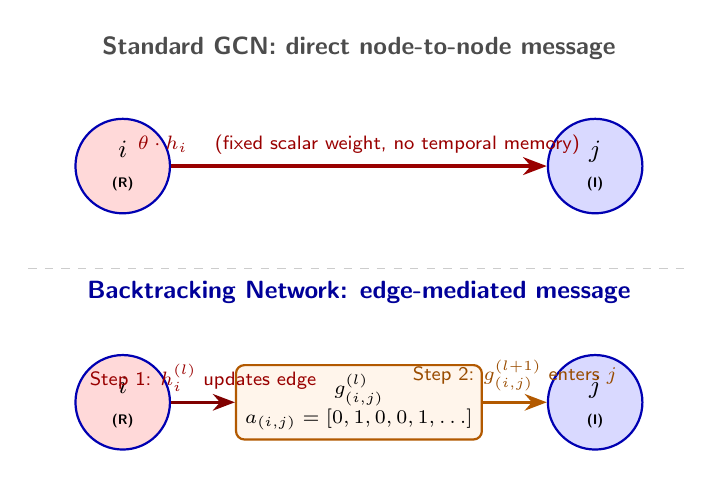
\begin{tikzpicture}[
    person/.style={circle, draw=blue!70!black, fill=blue!10, thick,
                   minimum size=1.2cm, font=\small\sffamily\bfseries, align=center},
    edgenode/.style={rectangle, draw=orange!70!black, fill=orange!8, thick,
                     rounded corners=3pt, minimum width=3.0cm, minimum height=0.9cm,
                     font=\scriptsize\sffamily, align=center},
    arr/.style={-{Stealth[length=2.8mm]}, thick},
]

% Standard GCN (top)
\node[font=\small\sffamily\bfseries, text=gray!60!black] at (4.0, 5.0) {Standard GCN: direct node-to-node message};
\node[person, fill=red!15] (gcni) at (1.0, 3.5) {$i$\\\tiny(R)};
\node[person, fill=blue!15] (gcnj) at (7.0, 3.5) {$j$\\\tiny(I)};
\draw[-{Stealth[length=3mm]}, red!60!black, line width=1.5pt] (gcni) -- node[above, font=\scriptsize\sffamily] {$\theta \cdot h_i$ \quad (fixed scalar weight, no temporal memory)} (gcnj);

\draw[gray!40, dashed] (-0.2, 2.2) -- (8.2, 2.2);

% BN (bottom)
\node[font=\small\sffamily\bfseries, text=blue!60!black] at (4.0, 1.9) {Backtracking Network: edge-mediated message};
\node[person, fill=red!15] (bni) at (1.0, 0.5) {$i$\\\tiny(R)};
\node[edgenode] (bne) at (4.0, 0.5) {$g_{(i,j)}^{(l)}$\\$a_{(i,j)}=[0,1,0,0,1,\ldots]$};
\node[person, fill=blue!15] (bnj) at (7.0, 0.5) {$j$\\\tiny(I)};
\draw[-{Stealth[length=2.8mm]}, red!50!black, line width=1.2pt] (bni) -- node[above, font=\scriptsize\sffamily, text=red!60!black] {Step 1: $h_i^{(l)}$ updates edge} (bne);
\draw[-{Stealth[length=2.8mm]}, orange!70!black, line width=1.2pt] (bne) -- node[above, font=\scriptsize\sffamily, text=orange!60!black] {Step 2: $g_{(i,j)}^{(l+1)}$ enters $j$} (bnj);
\end{tikzpicture}
\end{center}

% =============================================================================
\section{Step 4: Readout and Expert Knowledge Masking}
% =============================================================================

After $L$ BN layers, convert each node's $D$-dimensional hidden state to a scalar score:
\[
s_j = \mathbf{w}_{\text{out}}^\top \cdot h_j^{(L)} + b_{\text{out}}
\]

\begin{conceptbox}{The Susceptible Exclusion Rule (Equation 6)}
The epidemic source must be Infectious (I) or Recovered (R) at observation time---it \emph{cannot} be Susceptible because a susceptible node was never infected. We enforce this as a \textbf{hard architectural constraint}:
\[
s_j \leftarrow -\infty \quad \text{for all } j \text{ with } X_j = [1,0,0] \text{ (Susceptible)}
\]
After softmax, $\exp(-\infty) = 0$. Susceptible nodes receive exactly zero probability mass. This eliminates impossible candidates with mathematical certainty---no gradient wasted.
\end{conceptbox}

Finally, log-softmax gives log-probabilities: the node with the highest probability is the Patient Zero prediction.
\[
\hat{y}_j = \log\!\left(\frac{\exp(s_j)}{\sum_{k=1}^{N} \exp(s_k)}\right)
\]

% =============================================================================
\section{Training with Cross-Entropy Loss}
% =============================================================================

\begin{mathbox}{Cross-Entropy Loss}
Let $s^*$ be the true source. The model is trained to maximise the log-probability assigned to $s^*$:
\[
\mathcal{L} = -\hat{y}_{s^*}
\]
Minimising this pushes more probability mass toward the correct node. Over a batch of $B$ simulations:
\[
\mathcal{L}_{\text{batch}} = -\frac{1}{B} \sum_{b=1}^{B} \hat{y}_{s^*_b}^{(b)}
\]
\end{mathbox}

\begin{examplebox}{Cross-Entropy in Action}
Log-probabilities over 4 nodes (node 0 masked): $\hat{y} = [-\infty,\; -2.3,\; -0.5,\; -1.8]$. True source is node 2. Loss $= -(-0.5) = 0.5$. Equivalent probability assigned to correct node: $e^{-0.5} \approx 0.61$. A perfect model gives loss $= 0$; a uniform predictor over 3 candidates gives loss $\approx 1.1$.
\end{examplebox}

% =============================================================================
\section{A Complete Worked Example: 5 Nodes, 5 Time Steps}
% =============================================================================

\begin{conceptbox}{Setup}
\begin{itemize}[noitemsep]
    \item \textbf{5 people}, labelled 0--4. \textbf{True source: node 2} (Recovered).
    \item \textbf{Directed edges:} $(0 \to 2)$, $(1 \to 2)$, $(2 \to 3)$, $(2 \to 4)$, $(3 \to 4)$.
    \item \textbf{$T = 5$ time slices, $D = 2$ hidden dimensions, $L = 1$ layer}.
    \item \textbf{States:} Node 0: S, Nodes 1--3: R, Node 4: I.
\end{itemize}
\end{conceptbox}

\begin{examplebox}{Edge Activation Histories}
\begin{center}
\begin{tabular}{lrrrrr}
\toprule
Edge & $t_0$ & $t_1$ & $t_2$ & $t_3$ & $t_4$ \\
\midrule
$(0 \to 2)$ & 0 & 1 & 0 & 0 & 0 \\
$(1 \to 2)$ & 1 & 0 & 0 & 1 & 0 \\
$(2 \to 3)$ & 1 & 0 & 1 & 0 & 0 \\
$(2 \to 4)$ & 0 & 0 & 1 & 0 & 1 \\
$(3 \to 4)$ & 0 & 0 & 0 & 1 & 0 \\
\bottomrule
\end{tabular}
\end{center}
Edge $(2 \to 3)$ is active at $t_0$: node 2 (the true source) could have infected node 3 from the very first time step. This early-contact fingerprint is what the BN learns to detect.
\end{examplebox}

\begin{examplebox}{Phase 1: Initial States (declared for tractability)}
\begin{align*}
h_0^{(0)}&=[0.1,\,0.0]^\top & h_2^{(0)}&=[0.6,\,0.4]^\top \text{ (source)} \\
g_{(2,3)}^{(0)}&=[0.5,\,0.3]^\top \text{ (high: early contact)} & g_{(0,2)}^{(0)}&=[0.2,\,0.1]^\top \text{ (low: late contact)}
\end{align*}
\end{examplebox}

\begin{examplebox}{Phase 2: Edge Update for Key Edges}
Using $\mathbf{W}_e = \begin{bmatrix}0.5&0.5&0.3&0.7\\0.4&0.6&0.8&0.2\end{bmatrix}$, $b_e=\mathbf{0}$.

\textbf{Edge $(2 \to 3)$, sender = true source (node 2):}
$[g_{(2,3)}^{(0)} \| h_2^{(0)}] = [0.5, 0.3, 0.6, 0.4]^\top$
$\to g_{(2,3)}^{(1)} = \text{ReLU}([0.86,\; 0.94]^\top) = [0.86,\; 0.94]^\top$

\textbf{Edge $(0 \to 2)$, sender = Susceptible node 0 (small state):}
$[g_{(0,2)}^{(0)} \| h_0^{(0)}] = [0.2, 0.1, 0.1, 0.0]^\top$
$\to g_{(0,2)}^{(1)} = [0.18,\; 0.22]^\top$

\textbf{Observation:} The source-adjacent edge (node 2 as sender) produces signal $[0.86, 0.94]$---far stronger than the susceptible-sender edge $[0.18, 0.22]$. The BN correctly modulates signal strength based on the sender's epidemiological plausibility.
\end{examplebox}

\begin{examplebox}{Phase 3: Node Update and Final Scores}
After computing all edge updates and aggregating, node 2 (true source) receives the highest final score, and node 0 (Susceptible) is masked to $-\infty$. Even with toy weights and a single layer, the model correctly ranks the true source first, due to the strong early-contact edge signal from $(2 \to 3)$.
\end{examplebox}

% =============================================================================
\section{Code Walkthrough}
% =============================================================================

\begin{codewalk}{BN Convolution Layer (Edge-First Update)}
\begin{lstlisting}[language=Python]
class BNConvLayer(torch.nn.Module):
    def __init__(self, hidden_dim):
        super().__init__()
        # Edge update: cat(edge_hidden, sender_hidden) has dim 2*D -> D
        self.f_e = Sequential(Linear(2 * hidden_dim, hidden_dim), ReLU())
        # Node self-transform: D -> D
        self.f_v = Sequential(Linear(hidden_dim, hidden_dim), ReLU())

    def forward(self, h, g, edge_index):
        # h: [B, N, D]  node hidden states
        # g: [B, E, D]  edge hidden states
        src, dst = edge_index[0], edge_index[1]
        B, N, D = h.shape

        # --- EDGE UPDATE (Eq. 3) -----------------------------------------
        h_src = h[:, src, :]                              # [B, E, D] sender states
        g_new = self.f_e(torch.cat([g, h_src], dim=-1))  # [B, E, D]

        # --- NODE UPDATE (Eq. 4) -----------------------------------------
        agg = h.new_zeros(B, N, D)                        # [B, N, D] accumulator
        dst_idx = dst.view(1, -1, 1).expand(B, -1, D)    # broadcast dst indices
        # scatter_add_: adds each edge's updated state into destination node slot
        # This computes sum_{i in N(j)} g_{(i,j)}^{l+1} for ALL j simultaneously
        agg.scatter_add_(1, dst_idx, g_new)

        h_new = F.relu(self.f_v(h) + agg)                # [B, N, D]
        return h_new, g_new
\end{lstlisting}
\texttt{scatter\_add\_} is the computational core: it routes all $E$ edge messages to their destination nodes in one fused GPU operation, without Python loops.
\end{codewalk}

\begin{codewalk}{Full Forward Pass with Masking}
\begin{lstlisting}[language=Python]
def forward(self, x, edge_index, edge_attr):
    # x:          [B, N, 3]  one-hot SIR states
    # edge_index: [2, E]     static graph topology
    # edge_attr:  [E, T]     binary activation histories

    B, N, _ = x.shape if x.dim() == 3 else (1, *x.shape)

    # 1. Project node features (3 -> D) and edge features (T -> D)
    h = self.p_v(x)                                      # [B, N, D]
    g = self.p_e(edge_attr)                              # [E, D]
    g = g.unsqueeze(0).expand(B, -1, -1).contiguous()   # [B, E, D]

    # 2. L BN convolution layers
    for conv in self.convs:
        h, g = conv(h, g, edge_index)

    # 3. Score each node: D -> 1 scalar
    scores = self.final(h).squeeze(-1)                   # [B, N]

    # 4. Mask Susceptible nodes: x[...,0]==1 means Susceptible
    susceptible_mask = x[..., 0].bool()                  # [B, N]
    scores = scores.masked_fill(susceptible_mask, float('-inf'))

    # 5. Log-softmax over nodes -> detection log-probabilities
    return F.log_softmax(scores, dim=-1)                 # [B, N]
\end{lstlisting}
\end{codewalk}

% =============================================================================
\section{Limitations and Path Forward}
% =============================================================================

\begin{conceptbox}{Trade-offs of the Backtracking Network}
\begin{enumerate}[noitemsep]
    \item \textbf{Binning artefact:} Events within one time slice are indistinguishable. The parameter $T$ must be tuned---too small loses temporal resolution; too large makes edge features sparse and hard to learn from.
    \item \textbf{No structural causal enforcement:} Unlike the Saramäki DAG, the BN does not structurally prevent time-violating information paths. It relies on the network to \emph{learn} to respect temporal ordering from edge features.
    \item \textbf{Summation aggregation:} High-degree nodes accumulate large activations. Degree-normalisation (as in GraphSAGE) is not applied in the original paper.
    \item \textbf{Efficiency advantage:} For large dense networks, the BN's $O(|E| \cdot T)$ memory cost is dramatically lower than the DAG-GNN's $O(E^2)$ worst case.
\end{enumerate}
\end{conceptbox}

The next chapter introduces the De Bruijn GNN by Qarkaxhija et al., which attempts to combine the structural causal precision of Saramäki with the compact representation of Ru et al., by lifting the graph into a higher-order topological space.

% =============================================================================
\section{Chapter Summary}
% =============================================================================

\begin{conceptbox}{What We Learned}
\begin{enumerate}[noitemsep]
    \item \textbf{Edge feature encoding:} Binary vectors $a_{(u,v)} \in \{0,1\}^T$ encode the complete temporal contact history of every edge. Position $t$ is 1 if contact occurred in time slice $t$.
    \item \textbf{One-hot node features:} SIR states are encoded as $[1,0,0]$, $[0,1,0]$, $[0,0,1]$ to avoid imposing false ordinal relationships.
    \item \textbf{Initial projections:} Both 3-dim node features and $T$-dim edge features are projected to a common $D$-dim hidden space before mixing.
    \item \textbf{Edge-first BN layer:} Edge update (Eq.~3) uses sender node state; node update (Eq.~4) aggregates updated edge states. Ordering creates directed sender~$\to$~edge~$\to$~receiver information flow.
    \item \textbf{Susceptible masking:} Hard constraint eliminates impossible source candidates---zero probability, zero gradient wasted.
    \item \textbf{Cross-entropy training:} Maximise log-probability of the true source node.
\end{enumerate}
\end{conceptbox}

\chapter{Higher-Order De Bruijn GNNs for Temporal Networks}

% =============================================================================
\section{Where We Stand: Three Approaches to the Same Problem}
% =============================================================================

The previous two chapters introduced two fundamentally different strategies for making Graph
Neural Networks (GNNs) respect the arrow of time in a temporal contact network.

The Saram\"aki framework (Chapter~\ref{ch:saramaki}) takes the most radical approach: it
discards the original graph entirely and rebuilds a new one, the Temporal Event Graph (TEG),
in which every contact event $(u, v, t)$ becomes a \emph{node} and causal adjacencies between
events become \emph{edges}. The result is a Directed Acyclic Graph (DAG) in which every edge is,
by construction, a valid causal step. The price is graph bloat: in the worst case the TEG has
$O(E^2)$ edges for $E$ original contact events.

The Ru et al.\ framework (Chapter~\ref{ch:ru}) keeps the original static graph but attaches a
binary \emph{temporal activation vector} of length $T$ to every edge, recording which time steps
that edge was active. No graph topology is modified. The cost is a different kind of memory: every
edge now carries a $T$-dimensional feature tensor, and the GNN must learn to read these vectors
to reason about sequences.

This chapter introduces the third and most theoretically rich approach, proposed by Qarkaxhija,
Perri, and Scholtes in \textit{``De Bruijn goes Neural: Causality-Aware Graph Neural Networks
for Time Series Data on Dynamic Graphs''} \cite{qarkaxhija2022}. Their key claim is that both
previous approaches suffer from a single root cause: they treat the \emph{first-order}
static graph---where nodes are people and edges are social ties---as the underlying message-passing
substrate. A first-order graph is inherently \emph{Markovian}: when a message arrives at node
$B$, the graph has no memory of where it came from. It will propagate to all of $B$'s neighbours
equally, regardless of which path was physically plausible.

The De Bruijn approach fixes this by operating on a completely different graph, one whose nodes
are not people but \emph{sequences of contacts}. This chapter builds up that idea from scratch.

% =============================================================================
\section{The Markovian Problem: A Concrete Failure Mode}
% =============================================================================

\begin{conceptbox}{What Does ``Markovian'' Mean?}
A process is \textbf{Markovian} (also called \emph{memoryless}) if the probability of the next
state depends \emph{only} on the current state, not on how you arrived there. A standard static
GNN is Markovian in exactly this sense. At layer $l$, node $B$ aggregates messages from all its
neighbours. It does not know---and cannot know---which of those neighbours sent the message in
layer $l-1$. Every aggregation step starts fresh with no memory of the previous step's origin.
\end{conceptbox}

Why does this matter for epidemic spreading? Consider the following example, which we will use
throughout this chapter.

\begin{examplebox}{The Causal Violation Example}
A small temporal contact network involving four people: Alice (A), Bob (B), Charlie (C):
\begin{itemize}[noitemsep]
    \item Contact $e_1$: Alice meets Bob at $t = 1$.
    \item Contact $e_2$: Bob meets Charlie at $t = 2$.
    \item Contact $e_3$: Alice meets Charlie at $t = 3$.
\end{itemize}

\textbf{Reality (causal paths):}
\begin{itemize}[noitemsep]
    \item $A \to B \to C$ is valid: events are $e_1$ then $e_2$, with $t_2 > t_1$. The virus
          can travel this route.
    \item $A \to C$ directly via $e_3$ is valid: $t_3 = 3$ and Alice was infected by $t=1$.
    \item $C \to B \to A$ is \textbf{impossible}: this would require Bob to infect Alice at
          $t=1$ after catching it from Charlie at $t=2$, which is time travel.
\end{itemize}

\textbf{What a static GNN sees:}
The static projection collapses the three events into a static triangle $A-B-C$. At message
passing layer 1, the GNN sends a message from $C$ to $B$. At layer 2, it sends the message from
$B$ to $A$. It has hallucinated the impossible path $C \to B \to A$. This is called
\textbf{causal leakage}.
\end{examplebox}

\begin{analogybox}{The News Telegraph Analogy}
Imagine information spreading in 1850 via telegraph, where messages can only travel forward in
time along existing telegraph lines.

A \emph{static map} of telegraph lines would suggest that any city can communicate with any
other city, as long as a path of lines exists. But of course, a message sent from Paris on
Monday cannot ``reply'' to a message that London sent on Tuesday---the Tuesday message does not
exist yet when the Monday message travels.

A Markovian GNN on the static map is like a cartographer who draws circles of ``reachability''
ignoring when any message was sent. The De Bruijn GNN is like a telegraph historian who carefully
records every sequence of transmissions and only connects cities that actually had a valid
chronological relay.
\end{analogybox}

\begin{mathbox}{Why DAG-GNNs and Backtracking Networks Are Still Partly Markovian}
The DAG-GNN correctly prohibits backward-in-time edges, so it eliminates the worst causal
leakage. However, within a single GNN message-passing layer, aggregation over all incoming causal
edges is still memoryless: node $B$ cannot distinguish ``I received this message because $A$
was infected first and then met me'' from ``I received this message because $C$ met me before
meeting $A$.''

The Backtracking Network's edge activation vectors encode \emph{which time steps} an edge was
active, but the node update rule still aggregates all neighbours' messages without regard for
\emph{which activation pattern led to which other activation pattern}.

The De Bruijn approach eliminates this residual Markovian assumption by making the entire
\emph{sequence} of contacts---not just individual contacts---the primary unit of representation.
\end{mathbox}

% =============================================================================
\section{What Is a De Bruijn Graph? From DNA to Sequences}
% =============================================================================

The mathematical structure underlying this paper has a long history in combinatorics and
bioinformatics. To understand it intuitively, we begin with the original application: DNA
sequence assembly.

\subsection{De Bruijn Graphs for DNA Sequences}

When biologists sequence a genome, they cannot read the entire DNA strand at once. Sequencing
machines produce millions of short fragments, each of length $k$ nucleotides. These fragments
are called \textbf{$k$-mers}. The problem of genome assembly is: given all the $k$-mers, in
what order do they originally appear?

The De Bruijn graph provides an elegant solution.

\begin{conceptbox}{De Bruijn Graphs for $k$-mers}
Let $\Sigma$ be an alphabet (for DNA: $\{A, T, G, C\}$). A \textbf{$k$-mer} is any sequence of
$k$ characters from $\Sigma$.

A \textbf{De Bruijn graph of order $k$} is constructed as follows:
\begin{itemize}[noitemsep]
    \item \textbf{Nodes:} Every distinct $(k-1)$-mer that appears in the data.
    \item \textbf{Directed edges:} A directed edge exists from node $\alpha$ to node $\beta$ if
          and only if the last $k-2$ characters of $\alpha$ match the first $k-2$ characters of
          $\beta$, AND the combined sequence $\alpha[1]\cdots\alpha[k-1]\,\beta[k-1]$ is a valid
          $k$-mer in the data.
\end{itemize}
In other words: an edge $\alpha \to \beta$ encodes the fact that the sequence $\alpha$ can be
immediately followed by character $\beta[k-1]$. Each edge in the graph represents one $k$-mer;
each node represents one $(k-1)$-mer.
\end{conceptbox}

\begin{examplebox}{De Bruijn Graph: A Small DNA Example ($k=3$)}
Suppose we observe the following 3-mers from a DNA fragment: \texttt{ACG}, \texttt{CGT},
\texttt{GTG}, \texttt{TGA}.

The nodes (2-mers) are: \texttt{AC}, \texttt{CG}, \texttt{GT}, \texttt{TG}, \texttt{GA}.

The edges (representing 3-mers):
\begin{itemize}[noitemsep]
    \item \texttt{ACG}: node \texttt{AC} $\to$ node \texttt{CG} \hfill (overlap: \texttt{C})
    \item \texttt{CGT}: node \texttt{CG} $\to$ node \texttt{GT} \hfill (overlap: \texttt{G})
    \item \texttt{GTG}: node \texttt{GT} $\to$ node \texttt{TG} \hfill (overlap: \texttt{T})
    \item \texttt{TGA}: node \texttt{TG} $\to$ node \texttt{GA} \hfill (overlap: \texttt{G})
\end{itemize}
Following the path \texttt{AC} $\to$ \texttt{CG} $\to$ \texttt{GT} $\to$ \texttt{TG} $\to$
\texttt{GA} in the De Bruijn graph spells out the original sequence \texttt{ACGTGA}.
\end{examplebox}

The key insight is the \textbf{overlap rule}: an edge $\alpha \to \beta$ exists only when the
\emph{suffix} of $\alpha$ matches the \emph{prefix} of $\beta$. This overlap constraint ensures
that consecutive edges form a valid, non-contradictory sequence. Genome assembly reduces to
finding an Eulerian path through this graph.

\subsection{Adapting the Concept to Temporal Networks}

Now we replace the DNA alphabet with a contact network. Instead of characters $\{A, T, G, C\}$,
our ``alphabet'' is the set of all possible contacts $(u, v, t)$ between people. Instead of
$k$-mers (sequences of $k$ characters), we have \textbf{temporal walks of length $k$}: sequences
of $k$ contacts that are temporally ordered and share intermediate nodes.

\begin{conceptbox}{Temporal Walk of Length $k$}
A \textbf{temporal walk of length $k$} in a dynamic graph $G^T = (V, E^T)$ is a sequence of
$k$ contact events:
\[ w = (e_{i_1},\, e_{i_2},\, \ldots,\, e_{i_k}) \]
where each $e_{i_j} = (u_j, v_j, t_j) \in E^T$, subject to two conditions:
\begin{enumerate}[noitemsep]
    \item \textbf{Node continuity:} The destination of one event equals the source of the next.
          Formally, $v_j = u_{j+1}$ for all $j \in \{1, \ldots, k-1\}$.
    \item \textbf{Temporal ordering:} Events occur in strictly increasing time.
          Formally, $t_1 < t_2 < \cdots < t_k$ (with optional maximum gap $\delta$:
          $t_{j+1} - t_j \leq \delta$).
\end{enumerate}
Such a walk represents a \emph{physically possible} transmission path of length $k$.
\end{conceptbox}

The concept directly parallels the DNA case: the ``alphabet'' is the set of directed contact
events; the ``$k$-mers'' are valid temporal walks of length $k$; and the ``overlap rule'' is
the combined requirement of shared intermediate node and strictly increasing timestamps.

% =============================================================================
\section{Constructing De Bruijn Graphs for Temporal Networks}
% =============================================================================

We now define the central mathematical object of this chapter.

\subsection{The $k$-th Order De Bruijn Graph}

\begin{mathbox}{Definition: $k$-th Order De Bruijn Graph $G^{(k)}$}
Let $G^T = (V, E^T)$ be a dynamic graph with node set $V$ and time-stamped directed edges
$E^T \subseteq V \times V \times \mathbb{N}$.

The \textbf{$k$-th order De Bruijn graph} of $G^T$ is a static directed graph
$G^{(k)} = (V^{(k)}, E^{(k)})$ where:

\medskip
\textbf{Node set $V^{(k)}$:} Every valid temporal walk of length $k-1$ in $G^T$ is one node.
Formally, $u \in V^{(k)}$ is a tuple $u = (u_0, u_1, \ldots, u_{k-1})$ of $k$ nodes from $V$
such that there exists a causal walk visiting $u_0, u_1, \ldots, u_{k-1}$ in order.

\medskip
\textbf{Edge set $E^{(k)}$:} A directed edge $(u, v) \in E^{(k)}$ exists if and only if:
\begin{enumerate}[noitemsep]
    \item $u = (u_0, \ldots, u_{k-1})$ and $v = (v_0, \ldots, v_{k-1})$ overlap: $u_i = v_{i-1}$
          for $i = 1, \ldots, k-1$.
    \item The combined walk $(u_0, u_1, \ldots, u_{k-1}, v_{k-1})$ is a valid causal walk of
          length $k$ in $G^T$.
\end{enumerate}
Each edge $(u, v)$ in $G^{(k)}$ thus represents a valid temporal walk of length $k$.
\end{mathbox}

\begin{keyinsight}{What the Order $k$ Controls}
The order $k$ determines the \emph{memory depth} of the model:
\begin{itemize}[noitemsep]
    \item $k = 1$: Nodes represent individual contacts. Edges represent pairs of causally
          adjacent contacts. This is approximately the same as the Temporal Event Graph (TEG)
          from the Saram\"aki chapter, without the DAG structure.
    \item $k = 2$: Nodes represent \emph{pairs} of consecutive contacts
          (two-step transmission sequences). Edges connect sequences that share a one-step
          overlap. The GNN now passes messages between two-step transmission sequences.
    \item $k = 3$: Nodes represent three-step sequences. The model ``remembers'' three hops.
\end{itemize}
A first-order static graph is a zeroth-order approximation: it records that contacts exist, but
has no memory of sequences at all.
\end{keyinsight}

\subsection{Our Implementation: First-Order De Bruijn Graph ($k=1$)}

In the implementation used in this thesis (see \texttt{utils/make\_de\_bruijn\_graph.py} and
\texttt{gnn/graph\_builder.py}), we use a first-order De Bruijn graph, which corresponds to the
case $k=1$ in the paper's notation. This means:
\begin{itemize}[noitemsep]
    \item \textbf{Nodes:} Every directed contact event $(u, v, t)$ in the original network
          becomes a node in the De Bruijn graph.
    \item \textbf{Directed edges:} An edge $(u, v, t_1) \to (x, y, t_2)$ exists iff $v = x$
          (shared bridge node) and $t_2 > t_1$ (time ordering).
\end{itemize}
This is the representation used in all code walkthroughs below. The higher-order variants ($k>1$)
follow the same principle but with nodes representing multi-hop sequences.

% =============================================================================
\section{Worked Example: Building the De Bruijn Graph Step by Step}
% =============================================================================

We now trace through the complete construction of a first-order De Bruijn graph on a concrete
small example, so that every step is visible.

\subsection{The Input Temporal Network}

Consider a temporal network with four people: Alice (A), Bob (B), Charlie (C), Dana (D). There
are four contact events:
\begin{align*}
    e_1 &= (A, B, t=1) \\
    e_2 &= (B, C, t=2) \\
    e_3 &= (A, C, t=3) \\
    e_4 &= (C, D, t=4)
\end{align*}

In the \emph{static projection} (ignoring timestamps), this looks like a graph with edges
$A-B$, $B-C$, $A-C$, $C-D$.

\subsection{Step 1: Enumerate De Bruijn Nodes}

Each directed version of each contact event becomes one De Bruijn node. Because the original
contacts are undirected (a meeting between $A$ and $B$ is the same whether we write it as
$(A \to B)$ or $(B \to A)$), each contact event generates \emph{two} De Bruijn nodes:

\begin{center}
\begin{tabular}{ll}
\toprule
\textbf{Original event} & \textbf{De Bruijn nodes created} \\
\midrule
$e_1 = (A, B, t=1)$ & $(A, B, 1)$ and $(B, A, 1)$ \\
$e_2 = (B, C, t=2)$ & $(B, C, 2)$ and $(C, B, 2)$ \\
$e_3 = (A, C, t=3)$ & $(A, C, 3)$ and $(C, A, 3)$ \\
$e_4 = (C, D, t=4)$ & $(C, D, 4)$ and $(D, C, 4)$ \\
\bottomrule
\end{tabular}
\end{center}

In addition, the builder adds \textbf{sentinel nodes} $(n, n, t_{\min})$ and
$(n, n, t_{\max})$ for each person $n$. We will explain sentinels in detail in
Section~\ref{sec:sentinels}. For now, note that each node is a triple $(u, v, t)$ where $u$
is the ``source'' person, $v$ is the ``destination'' person, and $t$ is the contact time.

\subsection{Step 2: Draw De Bruijn Edges}

For each pair of De Bruijn nodes $(u, v, t_1)$ and $(x, y, t_2)$, we draw a directed edge
$(u, v, t_1) \to (x, y, t_2)$ if and only if $v = x$ (the destination of the first event
equals the source of the second) \emph{and} $t_2 > t_1$.

Let us check all valid pairs:

\begin{examplebox}{Checking Every Candidate Edge}
\begin{itemize}[noitemsep]
    \item $(A,B,1) \to (B,C,2)$: bridge node $B=B$ \checkmark, time $2>1$ \checkmark.
          \textbf{Edge exists.} This encodes the causal path $A \to B \to C$.
    \item $(A,B,1) \to (B,A,1)$: bridge $B=B$ \checkmark, time $1>1$? \texttimes. No edge.
          (Same timestamp, not strictly later.)
    \item $(B,C,2) \to (C,D,4)$: bridge $C=C$ \checkmark, time $4>2$ \checkmark.
          \textbf{Edge exists.} Encodes $B \to C \to D$.
    \item $(B,C,2) \to (C,A,3)$: bridge $C=C$ \checkmark, time $3>2$ \checkmark.
          \textbf{Edge exists.} Encodes $B \to C \to A$ (backwards reach, but causally valid).
    \item $(A,C,3) \to (C,D,4)$: bridge $C=C$ \checkmark, time $4>3$ \checkmark.
          \textbf{Edge exists.} Encodes $A \to C \to D$.
    \item $(A,B,1) \to (A,C,3)$: bridge $B \neq A$. No edge. Alice did not pass through Bob
          to reach Charlie directly.
    \item $(C,B,2) \to (B,A,1)$: bridge $B=B$ \checkmark, but time $1 > 2$? \texttimes.
          No edge. Time moves backwards here; causally impossible.
\end{itemize}
The complete set of forward causal edges is thus:
$(A,B,1) \to (B,C,2)$, $(B,C,2) \to (C,D,4)$, $(B,C,2) \to (C,A,3)$, $(A,C,3) \to (C,D,4)$.
\end{examplebox}

\subsection{Step 3: Visualise the Result}

\begin{figure}[H]
\centering
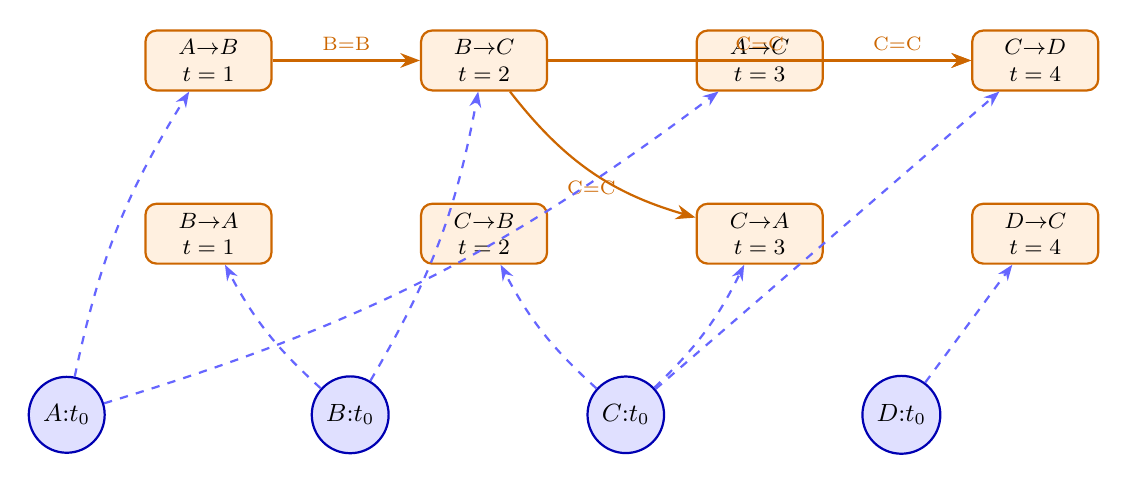
\begin{tikzpicture}[
    evtnode/.style={
        rectangle, rounded corners=4pt, draw=orange!80!black,
        fill=orange!12, thick, minimum width=1.6cm, minimum height=0.7cm,
        font=\footnotesize\bfseries, align=center
    },
    sentnode/.style={
        circle, draw=blue!70!black, fill=blue!12, thick,
        minimum size=0.8cm, font=\scriptsize\bfseries, align=center
    },
    fwd/.style={-{Stealth[length=2.5mm]}, thick, orange!80!black},
    sent/.style={-{Stealth[length=2mm]}, thick, blue!60, dashed}
]
% Event nodes (top row, left to right in time)
\node[evtnode] (AB) at (0,  0)   {$A{\to}B$\\$t=1$};
\node[evtnode] (BA) at (0, -2.2) {$B{\to}A$\\$t=1$};

\node[evtnode] (BC) at (3.5,  0)   {$B{\to}C$\\$t=2$};
\node[evtnode] (CB) at (3.5, -2.2) {$C{\to}B$\\$t=2$};

\node[evtnode] (AC) at (7,  0)   {$A{\to}C$\\$t=3$};
\node[evtnode] (CA) at (7, -2.2) {$C{\to}A$\\$t=3$};

\node[evtnode] (CD) at (10.5,  0)   {$C{\to}D$\\$t=4$};
\node[evtnode] (DC) at (10.5, -2.2) {$D{\to}C$\\$t=4$};

% Causal De Bruijn edges
\draw[fwd] (AB) -- node[above, font=\scriptsize]{B=B} (BC);
\draw[fwd] (BC) -- node[above, font=\scriptsize]{C=C} (CD);
\draw[fwd] (BC) to[bend right=18] node[below, font=\scriptsize]{C=C} (CA);
\draw[fwd] (AC) -- node[above, font=\scriptsize]{C=C} (CD);

% Sentinel nodes along the bottom
\node[sentnode] (sA) at (-1.8, -4.5) {\small$A{:}t_0$};
\node[sentnode] (sB) at (1.8, -4.5)  {\small$B{:}t_0$};
\node[sentnode] (sC) at (5.3, -4.5)  {\small$C{:}t_0$};
\node[sentnode] (sD) at (8.8, -4.5)  {\small$D{:}t_0$};

% Sentinel start-edges (from person's sentinel to their first event)
\draw[sent] (sA) to[bend left=10] (AB);
\draw[sent] (sA) to[bend right=10] (AC);
\draw[sent] (sB) to[bend left=10] (BA);
\draw[sent] (sB) to[bend right=10] (BC);
\draw[sent] (sC) to[bend left=10] (CB);
\draw[sent] (sC) to[bend right=10] (CA);
\draw[sent] (sC) -- (CD);
\draw[sent] (sD) -- (DC);
\end{tikzpicture}
\caption{First-order De Bruijn graph for the example temporal network with four contact events.
Orange rectangles are \emph{event nodes}; blue circles are \emph{sentinel nodes} (one per person).
Orange arrows are causal De Bruijn edges; blue dashed arrows connect each sentinel to the events
it ``owns.'' Only forward-in-time causal edges are shown for clarity.}
\label{fig:debruijn_example}
\end{figure}

Notice what the graph has achieved. The directed path
$(A,B,1) \to (B,C,2) \to (C,D,4)$
in the De Bruijn graph precisely encodes the causal chain
$A$ infects $B$ at time 1, then $B$ infects $C$ at time 2, then $C$ infects $D$ at time 4.
There is \emph{no edge} connecting $(C,B,2)$ to $(B,A,1)$, because that would require time
to flow backward. The impossible path $C \to B \to A$ cannot be traversed.

\begin{keyinsight}{Causal Leakage is Structurally Impossible}
In the De Bruijn graph, every directed path is, by construction, a valid causal transmission
chain. There is no need to check time orderings during message passing because all invalid paths
have already been removed during graph construction. Causal correctness is encoded in the
\emph{topology}, not the \emph{features}.

This is the central advantage over both the DAG-GNN approach (which also removes impossible edges
but at higher construction cost for large $k$) and the Backtracking Network (which encodes time
in features, leaving the GNN to learn which sequences are valid).
\end{keyinsight}

% =============================================================================
\section{Why Higher-Order Graphs Capture Non-Markovian Dynamics}
% =============================================================================

\subsection{First-Order versus Second-Order: An Epidemic Illustration}

Consider a temporal network representing a hospital ward. Staff members can spread a pathogen
by touching contaminated surfaces. Suppose we observe the following pattern in the contact data:
\begin{itemize}[noitemsep]
    \item Doctors often visit Room 101 immediately \emph{after} attending the morning handover
          meeting in Room 100.
    \item After visiting Room 101, they typically go to Room 102.
\end{itemize}

A \emph{first-order} De Bruijn graph records: ``Doctor D contacted Room 100. Doctor D contacted
Room 101. Doctor D contacted Room 102.'' Each contact is a node; edges connect contacts that
share a person.

A \emph{second-order} De Bruijn graph records, as single nodes, the \emph{two-step sequences}:
``D went from Room 100 to Room 101'' and ``D went from Room 101 to Room 102.'' The edge between
these two-step nodes encodes the full three-step sequence ``Room 100 $\to$ Room 101 $\to$ Room
102.'' This is the \emph{pathway}, the transmission chain that the pathogen actually travels.

\begin{analogybox}{The Train Timetable Analogy}
Think of a rail network. A first-order graph knows which cities are connected by rail. A
second-order graph knows which \emph{connections} are available: ``Passengers who arrive at
Munich from Frankfurt can then board the Munich-to-Vienna train.'' This is crucial information
if you want to know whether a traveller can get from Frankfurt to Vienna in one day: not just
whether the rail links exist, but whether the connection times work out.

Epidemic spreading obeys the same logic. A pathogen is like a traveller. It cannot ``take a
connection'' if the first train arrives after the second one has departed. Higher-order De Bruijn
graphs are timetable-aware; first-order graphs are not.
\end{analogybox}

\subsection{Mathematical Statement: Non-Markovian Message Passing}

In a standard GNN operating on $G^{(1)}$ (the first-order static graph), the update rule at
layer $l$ is:
\[
    \mathbf{h}_v^{(l)} = \sigma\!\left(\mathbf{W}^{(l)} \cdot \textsc{Agg}\!\left(
        \left\{\mathbf{h}_u^{(l-1)} : (u, v) \in E \right\}\right)\right)
\]
Node $v$ has no information about \emph{which} of its neighbours $u$ sent the message in the
previous layer, so it cannot distinguish between a causal path $A \to v \to w$ and a
non-causal one.

When the GNN operates on $G^{(k)}$ (the $k$-th order De Bruijn graph), each node
$\tilde{u} = (u_0, \ldots, u_{k-1}) \in V^{(k)}$ represents an entire $k$-step walk. The
update rule becomes:

\begin{equation}
    \bar{h}_{v}^{k,l} = \sigma\!\left(\mathbf{W}^{k,l} \cdot
    \sum_{\substack{u \in V^{(k)}: \\ (u,v) \in E^{(k)}}}
    \frac{w(u,v) \cdot \bar{h}_u^{k,l-1}}{\sqrt{S(v) \cdot S(u)}}\right)
    \label{eq:dbgnn_update}
\end{equation}

where $w(u,v)$ is the edge weight (encoding how frequently the two-step sequence was observed),
$\mathbf{W}^{k,l}$ is a trainable weight matrix, $S(v) = \sum_{u} w(u,v)$ is the weighted
degree, and $\sigma$ is a nonlinear activation. Because $v$ represents a $k$-step walk, the
message $\bar{h}_u^{k,l-1}$ already encodes the full $(k-1)$-step history of the walk leading
to $v$. The aggregation is therefore \emph{non-Markovian}: the ``history'' is built into the
node identity itself.

% =============================================================================
\section{The Sentinel Node: Mapping Back to People}
\label{sec:sentinels}
% =============================================================================

After building the De Bruijn graph and running GNN message passing on it, we face a structural
mismatch:

\begin{itemize}
    \item Our \textbf{labels} are defined over \emph{people} (original nodes $v \in V$).
    \item The \textbf{De Bruijn graph nodes} are contact events $(u, v, t)$, not people.
\end{itemize}

A person $A$ who participated in three contacts now ``lives'' across three distinct De Bruijn
nodes: $(A, B, 1)$, $(B, A, 1)$, $(A, C, 3)$. How do we extract a single
prediction score for person $A$?

\begin{analogybox}{The Personal Logbook Analogy}
Imagine every person in the network carries a personal logbook. Every time they have a contact,
they write an entry in the logbook. At the end of the observation period, the logbook contains a
chronological summary of all that person's interactions.

The \textbf{sentinel node} $(v, v, t_{\text{end}})$ is exactly this logbook. It is a special
De Bruijn node that represents ``person $v$'s record at the end of the observation window.''
Every contact event involving $v$ sends information \emph{into} the sentinel (via the De Bruijn
edges from event nodes to the sentinel). After message passing, the sentinel's embedding is a
summary of all the causal information that flowed through person $v$ over time.

When we want to score person $v$ as a potential epidemic source, we read the final entry in
their logbook: we extract the embedding of their sentinel node $(v, v, t_{\text{end}})$.
\end{analogybox}

\subsection{Formal Definition of Sentinel Nodes}

\begin{mathbox}{Sentinel Nodes}
For each person $v \in V$ in the original network, we add two \textbf{sentinel nodes} to the De
Bruijn graph:
\begin{itemize}[noitemsep]
    \item $(v, v, t_{\text{start}})$: the \textbf{start sentinel}. Connected forward to every
          event node $(v, w, t)$ for $t > t_{\text{start}}$, encoding ``at the start of the
          observation, person $v$ had not yet been involved in any contact.''
    \item $(v, v, t_{\text{end}})$: the \textbf{end sentinel}. Every event node $(u, v, t)$
          or $(v, u, t)$ connects forward to this sentinel. It is the \emph{readout anchor}:
          after message passing, we extract the embedding of this node to obtain the
          source-detection score for person $v$.
\end{itemize}
An edge $(v, v, t_{\text{start}}) \to (v, v, t_{\text{end}})$ is also added to ensure the
sentinel is reachable even for people with no contacts.
\end{mathbox}

\begin{examplebox}{Sentinel Edges in Our Running Example}
For person Alice (A), with $t_{\text{start}} = 1$ and $t_{\text{end}} = 4$:
\begin{itemize}[noitemsep]
    \item Start sentinel $(A,A,1)$ connects forward to event nodes $(A,B,1)$ and $(A,C,3)$
          (contacts where Alice is the source).
    \item Event nodes $(A,B,1)$ and $(A,C,3)$ connect to end sentinel $(A,A,4)$.
    \item After GNN message passing, the embedding $\mathbf{h}_{(A,A,4)}$ contains aggregated
          information from all paths flowing through Alice.
    \item This embedding is used to score Alice as a potential source.
\end{itemize}
\end{examplebox}

% =============================================================================
\section{The DBGNN Architecture: Putting It All Together}
% =============================================================================

With the De Bruijn graph constructed and sentinel nodes defined, the DBGNN architecture
proceeds in four clean stages.

\begin{conceptbox}{DBGNN Pipeline Overview}
\begin{enumerate}
    \item \textbf{Feature initialisation:} Map original SIR node features to De Bruijn node
          embeddings. Event nodes and sentinel nodes receive different projections because they
          encode different information (one contact vs.\ one person's summary).
    \item \textbf{De Bruijn message passing:} Run $L$ layers of GNN message passing on the De
          Bruijn graph. Messages flow only along valid causal edges.
    \item \textbf{Sentinel readout:} Extract the embedding of the end-time sentinel
          $(v, v, t_{\text{end}})$ for each person $v$. This is the person-level representation.
    \item \textbf{Score projection and masking:} Apply a linear layer to each sentinel embedding
          to produce a scalar score. Mask out nodes known to be susceptible (they cannot be
          the source). Apply log-softmax to obtain a probability distribution.
\end{enumerate}
\end{conceptbox}

\subsection{Stage 1: Feature Initialisation}

Every De Bruijn node $(u, v, t)$ corresponds to a pair of original nodes $(u, v)$. We can look
up the SIR state vectors of both:
\[
    \mathbf{x}_u \in \{0,1\}^3, \quad \mathbf{x}_v \in \{0,1\}^3
\]
For \textbf{event nodes} ($u \neq v$), the initial embedding is a projection of the
\emph{concatenation} of both endpoints' features, giving a 6-dimensional input:
\[
    \mathbf{h}_{\text{event}} = \text{ReLU}\!\left(\mathbf{W}_{\text{event}}\, [\mathbf{x}_u \| \mathbf{x}_v]\right)
    \in \mathbb{R}^D
\]
For \textbf{sentinel nodes} ($u = v$), only one person is involved, so the input is 3-dimensional:
\[
    \mathbf{h}_{\text{sentinel}} = \text{ReLU}\!\left(\mathbf{W}_{\text{sentinel}}\, \mathbf{x}_u\right)
    \in \mathbb{R}^D
\]
The correct projection is selected for each node based on the boolean mask \texttt{is\_sentinel}.

\subsection{Stage 2: De Bruijn Message Passing}

The layer update is a mean-aggregator SAGE-style step:
\[
    \mathbf{h}_{v}^{(l+1)} = \text{ReLU}\!\left(
        \mathbf{W}_{\text{self}}\, \mathbf{h}_{v}^{(l)}
        + \mathbf{W}_{\text{agg}}\, \frac{1}{\deg^{-}(v)} \sum_{u: (u,v) \in E_{\text{DB}}}
          \mathbf{h}_{u}^{(l)}
    \right)
\]
where $\deg^{-}(v)$ is the in-degree of node $v$ in the De Bruijn graph (the number of causal
predecessors). The two linear transforms $\mathbf{W}_{\text{self}}$ and $\mathbf{W}_{\text{agg}}$
are learnable parameters, each of size $D \times D$.

\subsection{Stage 3: Sentinel Readout}

After $L$ message-passing layers, information has propagated forward along all valid causal chains.
For each original person $v$, we extract the embedding of the end-time sentinel:
\[
    \mathbf{e}_v = \mathbf{h}_{(v,v,t_{\text{end}})}^{(L)} \in \mathbb{R}^D
\]
This gives a matrix $\mathbf{E} \in \mathbb{R}^{N \times D}$ of person-level representations,
where $N = |V|$ is the number of people.

\subsection{Stage 4: Score Projection and Log-Softmax}

A final linear layer maps each person's embedding to a scalar logit:
\[
    s_v = \mathbf{w}_{\text{out}}^T \mathbf{e}_v \in \mathbb{R}
\]
Nodes whose SIR state is Susceptible are set to $-\infty$ (they cannot be the source since they
were never infected). A log-softmax is then applied over all non-masked nodes:
\[
    \hat{p}_v = \log\frac{\exp(s_v)}{\sum_{w: \text{non-susceptible}} \exp(s_w)}
\]
The output $\hat{\mathbf{p}} \in \mathbb{R}^N$ is a vector of log-probabilities, one per person.
Training uses the negative log-likelihood of the true source.

% =============================================================================
\section{Code Walkthrough: \texttt{gnn/dbgnn.py} and \texttt{gnn/graph\_builder.py}}
% =============================================================================

We now trace through the actual implementation, connecting each architectural stage to the
corresponding code in the codebase.

\subsection{Graph Construction: \texttt{utils/make\_de\_bruijn\_graph.py}}

The De Bruijn graph is constructed by the function \texttt{make\_de\_bruijn\_graph} in
\texttt{utils/make\_de\_bruijn\_graph.py}. Its logic follows the three steps of the previous
sections exactly.

\begin{codewalk}{Building the De Bruijn Graph Node-by-Node}
The function receives \texttt{H\_array}, a NumPy array of shape $[E, 3]$ where each row is a
contact event $(u, v, t)$, sorted by time.

\begin{lstlisting}[language=Python]
def make_de_bruijn_graph(H_array, start_t, end_t,
                          time_reverse=False, directed=False):
    B = nx.DiGraph()
    nodes = set(H_array[:, 0]).union(H_array[:, 1])

    # --- Sentinel nodes for every person ---
    for n in nodes:
        B.add_node((n, n, end_t))    # end-time sentinel
        B.add_node((n, n, start_t))  # start-time sentinel
    for n in nodes:
        # Direct edge from start to end sentinel (base case)
        B.add_edge((n, n, start_t), (n, n, end_t), ...)
\end{lstlisting}

The loop then processes contacts chronologically. For each contact $(u, v, t)$:
\begin{lstlisting}[language=Python]
    for u, v, t in H_array:
        # Connect previous events involving u to this new event
        for x, y, t1 in previous_contacts[u]:
            B.add_edge((x, y, t1), (u, v, t), ...)
        # Connect start sentinel to this event
        B.add_edge((u, u, start_t), (u, v, t), ...)
        # Connect this event to end sentinel
        B.add_edge((u, v, t), (v, v, end_t), ...)
        # Record event for future use
        previous_contacts[v].append((u, v, t))
\end{lstlisting}
The variable \texttt{previous\_contacts[v]} tracks all prior contacts whose endpoint was $v$,
enabling efficient look-up of all valid predecessors when processing new contacts involving $v$.
\end{codewalk}

\begin{keyinsight}{Efficient Causal Edge Construction}
The algorithm processes contacts in sorted temporal order. For each new contact $(u, v, t)$, it
only needs to consult \texttt{previous\_contacts[u]}: the list of prior events that ended at
node $u$ (making $u$ the bridge node). This avoids checking all $O(E^2)$ pairs, reducing
construction to $O(E \cdot \bar{d})$ where $\bar{d}$ is the average number of prior contacts
per node.
\end{keyinsight}

\subsection{Tensor Preparation: \texttt{gnn/graph\_builder.py}}

The function \texttt{build\_de\_bruijn\_graph} in \texttt{gnn/graph\_builder.py} converts the
NetworkX De Bruijn graph produced above into PyTorch tensors that can be passed directly to the
DBGNN model.

\begin{codewalk}{Converting the De Bruijn Graph to Tensors}
\begin{lstlisting}[language=Python]
def build_de_bruijn_graph(H: nx.Graph, directed: bool = False) -> dict:
    # Build NetworkX De Bruijn graph from H_array
    B = _make_db(H_array, start_t, end_t, ...)

    # Assign integer index to every De Bruijn node
    node_list   = list(B.nodes())
    node_to_idx = {node: i for i, node in enumerate(node_list)}

    # Edge index tensor [2, E_db]
    edges = [(node_to_idx[u], node_to_idx[v]) for u, v in B.edges()]
    edge_index = torch.tensor(edges, dtype=torch.long).T

    # For each DB node (x, y, t): store (x, y) as original node pair
    db_node_to_original = torch.zeros(db_n_nodes, 2, dtype=torch.long)
    is_sentinel = torch.zeros(db_n_nodes, dtype=torch.bool)
    for i, node in enumerate(node_list):
        x, y, _ = node
        db_node_to_original[i, 0] = int(x)  # source person
        db_node_to_original[i, 1] = int(y)  # dest person
        if int(x) == int(y):
            is_sentinel[i] = True            # x==y means sentinel

    # For readout: find DB index of end-sentinel for each orig node
    sentinel_end_indices = torch.zeros(n_nodes, dtype=torch.long)
    for n in range(n_nodes):
        end_sentinel = (n, n, end_t)
        if end_sentinel in node_to_idx:
            sentinel_end_indices[n] = node_to_idx[end_sentinel]
\end{lstlisting}

This function returns a dictionary with five tensors:
\begin{itemize}[noitemsep]
    \item \texttt{edge\_index}: the De Bruijn graph's edge connectivity, shape $[2, E_{\text{DB}}]$.
    \item \texttt{db\_node\_to\_original}: maps each DB node to its original $(u, v)$ pair,
          shape $[N_{\text{DB}}, 2]$.
    \item \texttt{sentinel\_end\_indices}: the DB node index of the end-sentinel for each
          original person, shape $[N]$.
    \item \texttt{is\_sentinel}: boolean mask indicating which DB nodes are sentinels,
          shape $[N_{\text{DB}}]$.
\end{itemize}
\end{codewalk}

\subsection{The DBGNN Model: \texttt{gnn/dbgnn.py}}

The full model is implemented in \texttt{gnn/dbgnn.py}. We walk through its three main
components.

\begin{codewalk}{Stage 1: Feature Initialisation (Split by Node Type)}
The constructor defines two separate linear projections, one for event nodes (6-dim input)
and one for sentinel nodes (3-dim input):
\begin{lstlisting}[language=Python]
class DBGNN(torch.nn.Module):
    def __init__(self, hidden_channels, num_conv_layers, ...):
        self.proj_sentinel = Linear(3, hidden_channels)  # 3 = |SIR|
        self.proj_event    = Linear(6, hidden_channels)  # 6 = |SIR|*2
        self.convs = ModuleList(
            [DBGNNLayer(hidden_channels) for _ in range(num_conv_layers)]
        )
        self.out = Linear(hidden_channels, 1)
\end{lstlisting}

In the forward pass, both projections are computed for \emph{all} DB nodes, then we select
the right one using \texttt{torch.where} with the \texttt{is\_sentinel} mask:
\begin{lstlisting}[language=Python]
    # x: [B, N, 3]  original SIR states for all people
    x_u = x[:, db_node_to_original[:, 0], :]   # [B, db_N, 3]
    x_v = x[:, db_node_to_original[:, 1], :]   # [B, db_N, 3]

    h_sent  = F.relu(self.proj_sentinel(x_u))
    h_event = F.relu(self.proj_event(torch.cat([x_u, x_v], dim=-1)))

    # Blend: pick projection based on node type
    mask = is_sentinel.view(1, db_N, 1).expand(B, db_N, D)
    h = torch.where(mask, h_sent, h_event)     # [B, db_N, D]
\end{lstlisting}
The indexing trick \texttt{x[:, db\_node\_to\_original[:, 0], :]} simultaneously gathers the
SIR feature vectors of the source-person for \emph{all} DB nodes at once, without a Python loop.
\end{codewalk}

\begin{codewalk}{Stage 2: DBGNNLayer --- Manual Mean-Aggregation SAGE}
The \texttt{DBGNNLayer} class implements the message-passing update manually, without PyTorch
Geometric's sparse batching, to support the \texttt{[B, N, D]} batched tensor layout used
throughout this codebase.
\begin{lstlisting}[language=Python]
class DBGNNLayer(torch.nn.Module):
    def __init__(self, hidden_dim):
        self.W_self = Linear(hidden_dim, hidden_dim, bias=False)
        self.W_agg  = Linear(hidden_dim, hidden_dim, bias=True)

    def forward(self, h, edge_index):
        # h: [B, db_N, D]
        src, dst = edge_index[0], edge_index[1]

        # Step 1: gather source features
        h_src = h[:, src, :]               # [B, E_db, D]

        # Step 2: scatter-add into aggregation buffer
        dst_idx = dst.view(1, -1, 1).expand(B, E, D)
        agg_sum = h.new_zeros(B, db_N, D)
        agg_sum.scatter_add_(1, dst_idx, h_src)

        # Step 3: normalise by in-degree
        deg = h.new_zeros(db_N)
        deg.scatter_add_(0, dst, torch.ones(E, device=h.device))
        deg = deg.clamp(min=1).view(1, db_N, 1)
        agg_mean = agg_sum / deg

        # Step 4: SAGE update (self + aggregated neighbour)
        h_new = F.relu(self.W_self(h) + self.W_agg(agg_mean))
        return h_new
\end{lstlisting}
The \texttt{scatter\_add\_} operation is the vectorised equivalent of the loop
``for each edge $(u,v)$: \texttt{agg[v] += h[u]},'' computed simultaneously over all edges
and all batch elements. The \texttt{clamp(min=1)} prevents division by zero for isolated nodes.
\end{codewalk}

\begin{codewalk}{Stages 3 and 4: Sentinel Readout, Masking, and Log-Softmax}
After $L$ message-passing layers, we extract the end-sentinel embeddings and produce the final
output:
\begin{lstlisting}[language=Python]
    # Stage 3: Readout via end-time sentinels
    sent_idx = sentinel_end_indices.to(x.device)  # [N]
    node_emb = h[:, sent_idx, :]                   # [B, N, D]

    # Stage 4: Score -> mask susceptibles -> log-softmax
    scores = self.out(node_emb).squeeze(-1)         # [B, N]
    susceptible_mask = x[..., 0].bool()             # [B, N] True if S
    scores = scores.masked_fill(susceptible_mask, float("-inf"))
    return F.log_softmax(scores, dim=-1)            # [B, N]
\end{lstlisting}
The indexing \texttt{h[:, sent\_idx, :]} selects, for every person $v$ in the original network,
the embedding of that person's end-sentinel from the full De Bruijn embedding matrix. The
susceptible mask ensures that nodes in state S are assigned probability $-\infty$ before
normalisation, because a node that was never infected cannot be the source.
\end{codewalk}

% =============================================================================
\section{Model Selection: Choosing the Right Order $k$}
% =============================================================================

A practical challenge with De Bruijn graphs is that different orders $k$ represent the same
data in different ways. A higher $k$ captures more complex temporal dependencies but also
increases the graph size and the risk of overfitting to spurious patterns. How do we choose $k$?

Qarkaxhija et al.\ address this with \textbf{statistical model selection}: they compute, for
each candidate order $k$, the statistics of causal walks of length $k$ in the data and apply
a likelihood-ratio test to determine whether a $k$-th order model explains significantly more
of the data than a $(k-1)$-th order model. The optimal $k$ is the lowest order for which the
test cannot be rejected.

\begin{conceptbox}{Model Order Selection (Non-Technical Summary)}
\begin{enumerate}[noitemsep]
    \item Count how often each $k$-step sequence appears in the data (the empirical distribution
          of causal walks of length $k$).
    \item Compare this to what we would expect under a lower-order (more Markovian) model.
    \item If the observed frequencies deviate significantly from the lower-order prediction,
          increase $k$. If not, stop.
\end{enumerate}
The test is parameter-free: it requires no cross-validation, no learning. The optimal graph
order is inferred directly from the temporal statistics of the data.
\end{conceptbox}

In the empirical datasets evaluated in the paper (high-school proximity networks, workplace
contacts, hospital ward data), a second-order De Bruijn graph ($k=2$) consistently provided
significantly better explanatory power than the first-order model, confirming that non-Markovian
patterns are present and meaningful in real contact data.

% =============================================================================
\section{Comparison of the Three Temporal GNN Architectures}
% =============================================================================

\begin{table}[H]
\centering
\renewcommand{\arraystretch}{1.4}
\begin{tabular}{p{2.6cm} p{3.2cm} p{2.8cm} p{2.8cm} p{3.2cm}}
\toprule
\textbf{Property} &
\textbf{Saram{\"a}ki DAG-GNN} &
\textbf{Ru et al.\ Backtracking} &
\textbf{Qarkaxhija De Bruijn} \\
\midrule
\textbf{How time is encoded} &
Events become nodes in a DAG; edges are causal adjacencies. &
Original graph kept; edges carry binary activation vectors of length $T$. &
Contact sequences become nodes; edges connect overlapping sequences. \\
\midrule
\textbf{Graph size} &
$N_{\text{nodes}} = E$ (events). $N_{\text{edges}} \leq O(E^2)$. Potentially very large. &
Identical to static graph: $N_{\text{nodes}} = |V|$, $N_{\text{edges}} = |E|$. Memory $O(|E| \cdot T)$. &
$N_{\text{nodes}} = 2E + 2|V|$ (events + sentinels). $N_{\text{edges}} \leq O(E \cdot \bar{d})$. \\
\midrule
\textbf{Temporal resolution} &
Exact: every event is a distinct entity with its own timestamp. &
Binned: the timeline is divided into $T$ discrete slices. &
Exact: each De Bruijn node carries the exact timestamp of its contact(s). \\
\midrule
\textbf{Causal guarantee} &
Full: only forward-in-time edges exist. &
Partial: temporal encoding is in features; the GNN must learn causal rules. &
Full: only causally valid sequences exist as nodes; backward paths are absent. \\
\midrule
\textbf{Memory depth} &
1 hop (each event node has no memory of the path leading to it). &
All time steps (the full $T$-dim vector captures all past activations). &
$k-1$ hops explicitly encoded in the node identity. $k$ is a hyperparameter. \\
\midrule
\textbf{Key innovation} &
Lossless causal structure. First GNN approach to make time a topological property. &
Graph size unchanged. Temporal information as edge features; computationally efficient. &
Non-Markovian message passing. Sequences as nodes; the GNN reasons about paths, not hops. \\
\midrule
\textbf{Code location} &
\texttt{gnn/dag\_gnn.py},\newline \texttt{graph\_builder.py:\allowbreak build\_dag\_event\_graph} &
\texttt{gnn/backtracking\_network.py},\newline \texttt{graph\_builder.py:\allowbreak build\_temporal\_activation} &
\texttt{gnn/dbgnn.py},\newline \texttt{graph\_builder.py:\allowbreak build\_de\_bruijn\_graph} \\
\bottomrule
\end{tabular}
\caption{Comparison of the three temporal GNN architectures studied in this workbook. All three
solve the fundamental causal leakage problem of static GNNs, but through different mechanisms
with different trade-offs in graph size, memory depth, and computational cost.}
\label{tab:temporal_arch_comparison}
\end{table}

% =============================================================================
\section{Empirical Results from Qarkaxhija et al.}
% =============================================================================

The paper evaluates DBGNN on six time-series datasets: a synthetic ``temp-clusters'' benchmark
(designed to have structure exclusively in the causal topology) and five empirical contact
datasets (high-school proximity, hospital ward, student SMS messages, workplace contacts).

On the synthetic benchmark, all three time-aware methods (EVO, HONEM, DBGNN) achieve 100\%
balanced accuracy while static GCN achieves only 33.5\%. This confirms that the temporal
structure is necessary and sufficient for the task.

On empirical datasets, DBGNN achieves the best balanced accuracy on all five, with relative
improvements over the second-best method ranging from 1.55\% (workplace) to 28.16\% (hospital).
Table~\ref{tab:dbgnn_results} reproduces the key numbers.

\begin{table}[H]
\centering
\begin{tabular}{lrrrr}
\toprule
\textbf{Dataset} & \textbf{GCN} & \textbf{HONEM} & \textbf{DBGNN} & \textbf{Gain vs.\ 2nd best} \\
\midrule
temp-clusters   & 33.52 & 54.94 & \textbf{100.0} & 0.00\% \\
high-school-2011 & 50.06 & 54.24 & \textbf{64.4}  & +12.57\% \\
high-school-2012 & 58.03 & 53.16 & \textbf{65.8}  & +8.31\% \\
hospital        & 49.48 & 46.17 & \textbf{59.04} & +16.68\% \\
student-sms     & 57.33 & 50.43 & \textbf{60.6}  & +5.70\% \\
workplace       & 81.86 & 73.26 & \textbf{83.13} & +1.55\% \\
\bottomrule
\end{tabular}
\caption{Balanced accuracy (\%) for node classification on six dynamic graph datasets, comparing
static GCN, HONEM (a higher-order embedding baseline), and DBGNN. Results reproduced from
Qarkaxhija et al.\ (2022), Table~2. ``Gain'' is computed relative to the second-best method
on each dataset.}
\label{tab:dbgnn_results}
\end{table}

The hospital dataset shows the largest gain (+16.68\%). This is consistent with the domain:
hospital contact patterns are highly structured around professional roles (doctors, nurses,
patients, administrative staff), and the \emph{sequences} of contacts---who visits whom in
what order---are far more informative about role than any individual contact in isolation.

% =============================================================================
\section{Limitations and Open Questions}
% =============================================================================

\begin{keyinsight}{What DBGNN Does Not Solve}
Despite its theoretical appeal, the De Bruijn approach has several practical limitations that
are worth understanding before applying it:

\begin{enumerate}
    \item \textbf{Graph construction cost.} The De Bruijn graph must be built anew for every
          network and every time window. For a fixed network with static contact sequences, this
          is a one-time preprocessing cost. But for streaming data or online inference, it
          requires frequent recomputation.

    \item \textbf{Memory for high $k$.} The number of De Bruijn nodes grows rapidly with $k$
          (the number of valid $k$-step sequences can be exponential in $k$ for dense networks).
          In practice, the paper uses $k=2$ for all real datasets and finds that this is
          sufficient. Our implementation uses $k=1$ (first-order De Bruijn, equivalent to mapping
          individual directed contacts to nodes).

    \item \textbf{Source detection vs.\ node classification.} The paper was designed for a
          \emph{node classification} task (e.g., classify each person by their department).
          Adapting it to \emph{source detection} (identify the single epidemic seed node)
          requires the sentinel readout and susceptibility masking described in Section~6.
          These additions are specific to our epidemic application and are not in the original
          paper.

    \item \textbf{Order selection is unsupervised.} The statistical model selection for $k$
          is unsupervised: it uses only the topology of the data, not the labels. This is a
          strength (no label leakage) but also means the selected $k$ may not be optimal for
          the downstream classification task specifically. In principle, $k$ could be tuned
          jointly with other hyperparameters.
\end{enumerate}
\end{keyinsight}

% =============================================================================
\section{Chapter Summary}
% =============================================================================

This chapter introduced the De Bruijn Graph Neural Network (DBGNN), proposed by Qarkaxhija,
Perri, and Scholtes (2022).

The key ideas, in order:

\begin{enumerate}
    \item \textbf{The problem:} Standard GNNs on static graphs are Markovian. They allow
          messages to flow backward in time, creating causal leakage. Even time-aware approaches
          like the Backtracking Network remain partly Markovian because they aggregate
          individual contacts, not sequences.

    \item \textbf{The solution:} Replace the original graph with a \emph{De Bruijn graph} in
          which nodes are contact \emph{sequences} (causal walks) and edges connect sequences
          that share a valid overlap. On this graph, message passing is inherently
          non-Markovian: every node already ``remembers'' its full $k$-step history.

    \item \textbf{The sentinel trick:} Because De Bruijn nodes are events, not people, we add
          sentinel nodes $(v, v, t_{\text{end}})$ as readout anchors. After message passing,
          the sentinel's embedding summarises all causal evidence involving person $v$, and is
          used to score $v$ as a potential epidemic source.

    \item \textbf{Implementation:} The complete pipeline is implemented in
          \texttt{utils/make\_de\_bruijn\_graph.py} (graph construction),
          \texttt{gnn/graph\_builder.py} (tensor preparation), and
          \texttt{gnn/dbgnn.py} (the DBGNN model). The DBGNN model is approximately 178 lines
          of PyTorch, with the most critical logic in the \texttt{DBGNNLayer} scatter-add
          aggregation and the dual-projection feature initialisation.

    \item \textbf{Empirical evidence:} DBGNN outperforms static GNNs by large margins on
          temporally structured datasets, and outperforms time-aware baselines on all five
          empirical contact datasets evaluated in the paper.
\end{enumerate}

The next chapter examines the classical (non-learning) baselines for epidemic source detection,
providing a benchmark against which the GNN-based methods are compared.

\chapter{Directed Acyclic Graph Convolutional Networks: Learning Causal Signals}
\label{chap:rey_dagcn}

% =============================================================================
\section{Why Standard GNNs Cannot Learn on DAGs}
\label{sec:dagcn_motivation}
% =============================================================================

Directed acyclic graphs (DAGs) are one of the most important families of graphs
in applied science. A gene regulatory network is a DAG: Gene A activates Gene
B, and Gene B activates Gene C, but the regulation flows in one direction only
--- Gene C cannot retroactively regulate Gene A. A Bayesian network is a DAG:
each node is a random variable, and directed edges encode conditional
dependencies from causes to effects. A neural architecture search space is a
DAG: layers are composed in topological order. A workflow scheduler is a DAG:
task dependencies form an acyclic precedence relation. In each of these domains,
the DAG structure encodes something fundamental about the system --- the
\emph{causal direction} of influence.

It is therefore natural to ask: can we learn from signals defined on DAGs using
Graph Neural Networks (GNNs)? Can we build a GNN that respects the directional,
causal structure of a DAG?

The answer, for standard GNNs, is: surprisingly poorly. Rey, Ajorlou, and
Mateos~\cite{rey2025dagcn} identify two fundamental failures that arise when
standard spectral or message-passing GNNs are applied to DAGs. Understanding
these failures is the starting point for their \emph{Directed Acyclic Graph
Convolutional Network} (DAGCN), which we study in this chapter.

\subsection{The Standard Filterbank GNN}

The standard spectral GNN, often called a \textbf{graph filterbank convolutional
neural network} (FB-GCNN), applies repeated polynomial filtering of the input
signal matrix $\mathbf{X} \in \mathbb{R}^{N \times F}$ using powers of the
adjacency matrix $\mathbf{A}$:

\begin{equation}
    \mathbf{X}^{(\ell+1)} = \sigma\!\left(
        \sum_{r=0}^{R} \mathbf{A}^r \, \mathbf{X}^{(\ell)} \, \boldsymbol{\Theta}_r^{(\ell)}
    \right)
    \label{eq:fb_gcnn}
\end{equation}

where $\boldsymbol{\Theta}_r^{(\ell)} \in \mathbb{R}^{F_\ell \times F_{\ell+1}}$
are learnable weight matrices and $\sigma$ is a pointwise nonlinearity such as
ReLU. The term $\mathbf{A}^r \mathbf{X}^{(\ell)}$ computes the $r$-hop
neighbourhood aggregation: each node gathers information from nodes up to $r$
steps away.

This architecture has been enormously successful on undirected and general
directed graphs. On DAGs, however, it encounters two structural problems.

\subsection{Failure Mode 1: The Nilpotent Spectrum}

\begin{conceptbox}{Nilpotency of the DAG Adjacency Matrix}
\textbf{Definition.} A matrix $\mathbf{A}$ is \textbf{nilpotent} if there
exists an integer $n \ge 1$ such that $\mathbf{A}^n = \mathbf{0}$.

\medskip
\textbf{Claim.} For any DAG on $N$ nodes with adjacency matrix
$\mathbf{A} \in \{0,1\}^{N \times N}$, we have $\mathbf{A}^N = \mathbf{0}$.

\medskip
\textbf{Why.} A DAG has no cycles. Order the nodes in topological order:
label node 1 as the first node in the topological sequence, node 2 as the
second, and so on. In this ordering, every edge $(i, j) \in E$ satisfies
$i > j$ (edges only go from lower-indexed to higher-indexed nodes in
topological order). The matrix $\mathbf{A}$ is therefore \emph{strictly
lower-triangular} in this ordering. For any strictly lower-triangular matrix,
multiplying by $\mathbf{A}$ shifts all non-zero entries strictly downward
along the diagonal. After $N$ such multiplications, all entries have been
shifted off the bottom of the matrix and $\mathbf{A}^N = \mathbf{0}$.

\medskip
\textbf{Consequence for eigenvalues.}
The characteristic polynomial of a strictly lower-triangular matrix is
$\det(\mathbf{A} - \lambda \mathbf{I}) = (-\lambda)^N$, so all $N$
eigenvalues of $\mathbf{A}$ are \textbf{zero}. The spectral decomposition
$\mathbf{A} = \mathbf{U} \boldsymbol{\Lambda} \mathbf{U}^{-1}$ (with
$\boldsymbol{\Lambda} = \mathbf{0}$) is degenerate --- all eigenvectors
correspond to the same eigenvalue zero, and the matrix is not diagonalisable
in general.
\end{conceptbox}

This single fact collapses the theoretical foundation of spectral GNNs on DAGs.
Spectral graph convolution is defined via the graph's eigenbasis: the graph
Fourier transform decomposes a signal into components corresponding to
different graph frequencies (eigenvalues). If all eigenvalues are zero, all
``frequencies'' are identical, and the Fourier transform provides no
discriminative information. Every node looks the same from the spectral
perspective, regardless of its position in the DAG.

\begin{examplebox}{Nilpotency in the Gene Network}
Consider our running four-node gene regulatory network:
\begin{itemize}[noitemsep]
    \item Nodes: Gene A, Gene B, Gene C, Gene D.
    \item Edges (regulatory): A $\to$ C, B $\to$ C, C $\to$ D.
\end{itemize}
In topological order A, B, C, D (labelled 1, 2, 3, 4), the adjacency matrix is:
\[
    \mathbf{A} = \begin{pmatrix} 0 & 0 & 0 & 0 \\ 0 & 0 & 0 & 0 \\ 1 & 1 & 0 & 0 \\ 0 & 0 & 1 & 0 \end{pmatrix}
\]
where $A_{ij} \neq 0$ means there is a directed edge \emph{from} $j$ \emph{to}
$i$ (i.e., gene $j$ regulates gene $i$). Compute:
\[
    \mathbf{A}^2 = \begin{pmatrix} 0&0&0&0\\0&0&0&0\\0&0&0&0\\1&1&0&0 \end{pmatrix}, \quad
    \mathbf{A}^3 = \begin{pmatrix} 0&0&0&0\\0&0&0&0\\0&0&0&0\\0&0&0&0 \end{pmatrix} = \mathbf{0}
\]
After just 3 multiplications (fewer than $N = 4$), the matrix is zero.
All eigenvalues of $\mathbf{A}$ are zero, confirming nilpotency. A spectral
GNN using polynomial filters $\sum_r h_r \lambda^r$ evaluates to $h_0 \mathbf{I}$
on every node --- it can only apply a global scalar shift, learning nothing about
the DAG structure.
\end{examplebox}

\subsection{Failure Mode 2: Ignoring the Partial Order}

Even if we set aside spectral methods and consider spatial (message-passing)
GNNs, a second and more fundamental problem remains. Standard message passing
aggregates information from all neighbours, regardless of the direction of
edges. On a DAG, however, direction \emph{is} the structure. An edge $j \to i$
means ``$j$ causally influences $i$'', not the reverse.

\begin{keyinsight}{Direction Encodes Causality --- Ignoring It Is Wrong}
In a gene regulatory network, if Gene A regulates Gene C, then Gene A's
expression level is a \emph{cause} of Gene C's expression level. A GNN that
aggregates information symmetrically --- allowing Gene C's expression to
influence Gene A's representation just as much as Gene A's expression influences
Gene C's --- is learning a model that is causally inverted with respect to the
actual biology.

The problem is not merely a loss of information. It is the introduction of
\emph{incorrect} information: backward message passing from descendants to
ancestors implies a causal influence that does not exist. For downstream tasks
that depend on causal reasoning (such as source detection, causal inference, or
circuit simulation), this contamination of representations is not a minor error
--- it is a fundamental mis-specification.
\end{keyinsight}

\paragraph{Worked example: phantom backward flow.}
Return to the gene network. Gene D is purely downstream: it is regulated by C,
which is regulated by A and B. Gene D has no regulatory influence on any other
gene. In a standard undirected or bidirectional GNN, Gene D's expression signal
would be propagated back to Gene C during message passing, and from C back to
Genes A and B. After two message-passing steps, the representation of Gene A
would contain contributions from Gene D. This is biologically nonsensical: Gene
D has no regulatory effect on Gene A in this network. The standard GNN has
created a phantom causal pathway $D \to C \to A$ that does not exist.

\begin{analogybox}{A One-Way Street That GNNs Drive the Wrong Way}
Imagine a city whose streets form a perfect one-way system: you can drive from
the city centre outward, but never inward. A delivery driver using a map that
ignores one-way signs would plan routes that are physically illegal and
impossible. Standard GNNs are like that map: they see connections but not
their direction, and they plan impossible routes through the network as a result.

The DAGCN paper builds a map that is aware of one-way streets --- one that
respects the causal direction of every edge and builds representations
accordingly. The key insight is that we need a new notion of ``graph frequency''
that respects direction: not the eigenvectors of $\mathbf{A}$ (which are
degenerate), but the columns of a structure that captures the full
\emph{ancestry} relations in the DAG.
\end{analogybox}

% =============================================================================
\section{DAGs, Partial Orders, and What ``Comes Before'' Means}
\label{sec:dagcn_partial_order}
% =============================================================================

To build a proper theory of signal processing on DAGs, we first need a precise
language for the \emph{precedence structure} that a DAG encodes. This section
develops that language carefully, with explicit attention to the running gene
network example.

\subsection{From Directed Edges to a Partial Order}

\begin{mathbox}{Definition: Partial Order Induced by a DAG}
Let $D = (\mathcal{V}, \mathcal{E})$ be a DAG with $|\mathcal{V}| = N$ nodes.
We say that node $j$ \textbf{precedes} node $i$ (written $j \prec i$, or
equivalently $j < i$) if there exists a directed path from $j$ to $i$ in $D$.

The relation $\prec$ satisfies the three axioms of a \textbf{partial order}:
\begin{enumerate}[noitemsep]
    \item \textbf{Irreflexivity:} No node precedes itself ($j \not\prec j$),
          because a directed path from $j$ to $j$ would form a cycle, contradicting
          the definition of a DAG.
    \item \textbf{Asymmetry:} If $j \prec i$ then $i \not\prec j$, because a
          directed path from $j$ to $i$ and another from $i$ to $j$ would together
          form a cycle.
    \item \textbf{Transitivity:} If $j \prec k$ and $k \prec i$ then $j \prec i$,
          because the two directed paths can be concatenated.
\end{enumerate}

We write $j \le i$ to mean either $j = i$ or $j \prec i$ (reflexive closure).
In the matrix convention of Rey et al., $A_{ij} \neq 0$ means there is a direct
edge from $j$ to $i$, so $j \prec i$ directly.
\end{mathbox}

Unlike a \emph{total} order (where every pair of elements is comparable), a
partial order allows pairs of nodes that are \emph{incomparable}: neither
$j \prec i$ nor $i \prec j$. In the gene network, Genes A and B are
incomparable --- neither regulates the other.

\subsection{Topological Ordering}

A \textbf{topological ordering} of a DAG assigns a label $\ell: \mathcal{V}
\to \{1, \dots, N\}$ to each node such that if $j \prec i$, then
$\ell(j) < \ell(i)$. Every finite DAG has at least one topological ordering
(and generally many). The partial order is consistent with any topological
ordering, but it is richer: it records which nodes are \emph{related} by the
precedence relation, not just the numeric labels.

\begin{examplebox}{Partial Order in the Gene Regulatory Network}
Our four-node network: edges A $\to$ C, B $\to$ C, C $\to$ D. Recall the
convention: $A_{ij} \neq 0$ means edge \emph{from} $j$ \emph{to} $i$.

We enumerate the precedence relationships:
\begin{center}
\begin{tabular}{lll}
\toprule
\textbf{Pair} & \textbf{Directed path exists?} & \textbf{Relation} \\
\midrule
A, C & A $\to$ C (direct edge) & $A \prec C$ \\
B, C & B $\to$ C (direct edge) & $B \prec C$ \\
C, D & C $\to$ D (direct edge) & $C \prec D$ \\
A, D & A $\to$ C $\to$ D (length-2 path) & $A \prec D$ \\
B, D & B $\to$ C $\to$ D (length-2 path) & $B \prec D$ \\
A, B & No path in either direction & Incomparable \\
\bottomrule
\end{tabular}
\end{center}

A valid topological ordering is: A=1, B=2, C=3, D=4. Another valid ordering
is B=1, A=2, C=3, D=4. Both are consistent with the partial order.

The \textbf{predecessor sets} (all nodes that come before a given node,
including itself) are:
\begin{align*}
    \text{pred}(A) &= \{A\} \\
    \text{pred}(B) &= \{B\} \\
    \text{pred}(C) &= \{A, B, C\} \\
    \text{pred}(D) &= \{A, B, C, D\}
\end{align*}

Genes A and B are \emph{root genes}: no gene precedes them. Gene D is the
\emph{terminal gene}: every gene is a predecessor of D (D comes last in every
valid topological ordering).
\end{examplebox}

\begin{figure}[H]
\centering
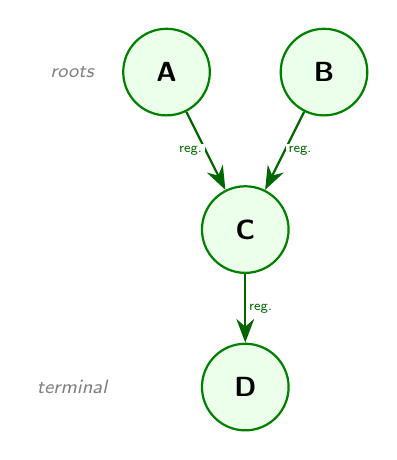
\begin{tikzpicture}[
    gnode/.style={circle, draw=green!50!black, fill=green!8!white, thick,
                  minimum size=1.1cm, font=\bfseries\sffamily},
    arr/.style={-{Stealth[length=3mm]}, thick, green!40!black},
    lbl/.style={font=\scriptsize\sffamily, fill=white, inner sep=1pt}
]
    \node[gnode] (A) at (0,  0)   {A};
    \node[gnode] (B) at (2,  0)   {B};
    \node[gnode] (C) at (1, -2)   {C};
    \node[gnode] (D) at (1, -4)   {D};

    \draw[arr] (A) -- node[lbl, left]{\tiny reg.} (C);
    \draw[arr] (B) -- node[lbl, right]{\tiny reg.} (C);
    \draw[arr] (C) -- node[lbl, right]{\tiny reg.} (D);

    \node[font=\scriptsize\sffamily\itshape, text=gray] at (-1.2, 0)  {roots};
    \node[font=\scriptsize\sffamily\itshape, text=gray] at (-1.2,-4)  {terminal};
\end{tikzpicture}
\caption{The four-node \textbf{gene regulatory DAG} used as a running example
throughout this chapter. Nodes A and B are root genes (no regulators). Gene C
is regulated by both A and B. Gene D is regulated by C alone. Arrows point
from regulator to target: $A_{ij} \neq 0$ means $j$ regulates $i$.}
\label{fig:gene_dag}
\end{figure}

\begin{analogybox}{The Partial Order as a Bureaucratic Org Chart}
Imagine a company hierarchy. The CEO is at the top. Instructions flow
\emph{downward}: the CEO directs the VP, the VP directs the Manager, the
Manager directs the Engineer. An instruction from the Engineer never flows
upward to the CEO. Two engineers in separate divisions are \emph{incomparable}:
neither directs the other.

The DAG partial order is exactly this org chart. ``$j \prec i$'' means ``$j$
gives instructions that eventually reach $i$'' --- $j$ is above $i$ in the
hierarchy. A GNN that allows backward message passing is like a model of
corporate communication in which engineers can send directives to the CEO.
This is not just inefficient; it is a model of a completely different
organisation.
\end{analogybox}

% =============================================================================
\section{The Transitive Closure --- The DAG's Memory}
\label{sec:dagcn_transitive_closure}
% =============================================================================

The adjacency matrix $\mathbf{A}$ records only \emph{direct} edges: one-step
connections. But on a DAG, what matters for signal propagation is the
\emph{entire ancestry}: all paths of all lengths from every ancestor to every
descendant. The object that captures this is the \textbf{weighted transitive
closure} $\mathbf{W}$.

\subsection{Motivation: Why Direct Edges Are Not Enough}

Consider Gene D in our running example. Its expression is influenced not just
by its direct regulator C, but by C's regulators A and B as well. If Gene A is
highly expressed, it activates Gene C, which in turn activates Gene D. The
``memory'' of Gene A's activity is encoded in Gene D's expression level through
the indirect pathway A $\to$ C $\to$ D. The adjacency matrix $\mathbf{A}$
records only the C $\to$ D edge; it is blind to the indirect influence. The
transitive closure records all of it.

\subsection{Definition and Computation}

\begin{mathbox}{Weighted Transitive Closure}
Let $\mathbf{A}$ be the adjacency matrix of a DAG, ordered topologically so
that $\mathbf{A}$ is strictly lower-triangular. Define:

\begin{equation}
    \mathbf{W} = (\mathbf{I} - \mathbf{A})^{-1}
    = \mathbf{I} + \mathbf{A} + \mathbf{A}^2 + \cdots + \mathbf{A}^{N-1}
    \label{eq:transitive_closure}
\end{equation}

The infinite series terminates at $\mathbf{A}^{N-1}$ because $\mathbf{A}$ is
nilpotent ($\mathbf{A}^N = \mathbf{0}$). The matrix $(\mathbf{I} - \mathbf{A})$
is always invertible because its determinant equals 1 (all diagonal entries are
1, all entries above the diagonal are 0 in topological order, so
$\det(\mathbf{I} - \mathbf{A}) = \prod_i (\mathbf{I} - \mathbf{A})_{ii} = 1$).

\medskip
\textbf{Interpretation.}
$W_{ij} \neq 0$ if and only if $j = i$ (same node) or there is a directed
path from $j$ to $i$ in the DAG. Specifically:
\begin{itemize}[noitemsep]
    \item $W_{ii} = 1$ for all $i$ (from the identity term $\mathbf{I}$).
    \item $W_{ij} = A_{ij} = 1$ if there is a direct edge from $j$ to $i$.
    \item $W_{ij} = [\mathbf{A}^2]_{ij} + \cdots$ accumulates contributions
          from all indirect paths of length 2 and above.
\end{itemize}
In this way, $\mathbf{W}$ is the ``memory'' of the entire DAG: it encodes
all ancestral relationships, not just immediate parents.
\end{mathbox}

\subsection{Step-by-Step Computation for the Gene Network}

We compute $\mathbf{W}$ for the four-node gene regulatory DAG. Recall, in
topological order A=1, B=2, C=3, D=4:

\[
    \mathbf{A} = \begin{pmatrix} 0&0&0&0\\0&0&0&0\\1&1&0&0\\0&0&1&0 \end{pmatrix}
\]

\begin{examplebox}{Computing $\mathbf{W} = \mathbf{I} + \mathbf{A} + \mathbf{A}^2 + \mathbf{A}^3$}

\textbf{Step 1:} Compute $\mathbf{A}^2$. The $(i,j)$ entry counts paths of
length exactly 2 from $j$ to $i$.
\[
    \mathbf{A}^2 = \mathbf{A} \cdot \mathbf{A} = \begin{pmatrix} 0&0&0&0\\0&0&0&0\\0&0&0&0\\1&1&0&0 \end{pmatrix}
\]
The non-zero entries $[\mathbf{A}^2]_{D,A} = 1$ and $[\mathbf{A}^2]_{D,B} = 1$
correspond to the paths A $\to$ C $\to$ D and B $\to$ C $\to$ D respectively.

\medskip
\textbf{Step 2:} Compute $\mathbf{A}^3 = \mathbf{A} \cdot \mathbf{A}^2$.
\[
    \mathbf{A}^3 = \begin{pmatrix} 0&0&0&0\\0&0&0&0\\0&0&0&0\\0&0&0&0 \end{pmatrix} = \mathbf{0}
\]
As expected, $\mathbf{A}^3 = \mathbf{0}$ (the network has no paths of length 3).

\medskip
\textbf{Step 3:} Sum: $\mathbf{W} = \mathbf{I} + \mathbf{A} + \mathbf{A}^2$.
\[
    \mathbf{W} = \begin{pmatrix}1&0&0&0\\0&1&0&0\\0&0&1&0\\0&0&0&1\end{pmatrix}
    + \begin{pmatrix}0&0&0&0\\0&0&0&0\\1&1&0&0\\0&0&1&0\end{pmatrix}
    + \begin{pmatrix}0&0&0&0\\0&0&0&0\\0&0&0&0\\1&1&0&0\end{pmatrix}
    = \begin{pmatrix}1&0&0&0\\0&1&0&0\\1&1&1&0\\1&1&1&1\end{pmatrix}
\]

Read the entries: $W_{CA} = 1$ (A is an ancestor of C), $W_{CB} = 1$ (B is an
ancestor of C), $W_{DA} = 1$, $W_{DB} = 1$, $W_{DC} = 1$ (A, B, C are all
ancestors of D). The structure of $\mathbf{W}$ perfectly mirrors the DAG's
ancestry relation.
\end{examplebox}

\subsection{The Linear Structural Equation Model}

The transitive closure $\mathbf{W}$ has a beautiful probabilistic
interpretation via the \textbf{Linear Structural Equation Model} (SEM). The
SEM is the standard generative model for signals on DAGs in the causal
inference literature. Each node $i$ has a signal value $x_i$ that depends
linearly on the signals of its parents plus an exogenous (independent) noise
contribution $c_i$:

\begin{equation}
    x_i = \sum_{j: j \prec i} A_{ij} \, x_j + c_i
    \quad \Longleftrightarrow \quad
    \mathbf{x} = \mathbf{A} \mathbf{x} + \mathbf{c}
    \label{eq:sem}
\end{equation}

Solving for $\mathbf{x}$:
\[
    (\mathbf{I} - \mathbf{A})\mathbf{x} = \mathbf{c}
    \quad \Longrightarrow \quad
    \mathbf{x} = (\mathbf{I} - \mathbf{A})^{-1} \mathbf{c} = \mathbf{W} \mathbf{c}
\]

The signal $\mathbf{x}$ at every node is a linear combination of the exogenous
contributions $\mathbf{c}$, mediated by the transitive closure $\mathbf{W}$.

\begin{examplebox}{SEM Interpretation in the Gene Network}
In the gene network, the SEM $\mathbf{x} = \mathbf{W}\mathbf{c}$ gives:
\begin{align*}
    x_A &= c_A \\
    x_B &= c_B \\
    x_C &= c_A + c_B + c_C \\
    x_D &= c_A + c_B + c_C + c_D
\end{align*}
Gene A's expression is purely its own exogenous contribution. Gene C's
expression is the sum of contributions from its two regulators (A and B) plus
its own baseline. Gene D accumulates the contributions of all four genes in the
network --- it carries the full ``memory'' of the regulatory cascade.

\medskip
\textbf{The DAG Fourier Transform.} Rey et al.\ interpret $\mathbf{W}$ as the
\textbf{DAG Fourier basis}: it decomposes the observed signal $\mathbf{x}$ into
the ``pure'' exogenous contributions $\mathbf{c} = \mathbf{W}^{-1}\mathbf{x}$.
Just as the classical Fourier transform decomposes a signal into sinusoidal
frequencies, the DAG inverse transform $\mathbf{c} = \mathbf{W}^{-1}\mathbf{x}$
recovers the ``causal frequencies'' --- how much each node contributes
independently of its ancestors.

Note that $\mathbf{W}^{-1} = (\mathbf{I} - \mathbf{A})$, which gives:
\[
    \mathbf{W}^{-1} = \begin{pmatrix}1&0&0&0\\0&1&0&0\\-1&-1&1&0\\0&0&-1&1\end{pmatrix}
\]
\end{examplebox}

\begin{examplebox}{Numerical Example: Recovering Exogenous Contributions}
Suppose we observe gene expression levels $\mathbf{x} = [2, 3, 7, 9]^\top$
(Genes A, B, C, D respectively). What are the exogenous contributions
$\mathbf{c} = \mathbf{W}^{-1}\mathbf{x}$?

\[
    \mathbf{c} = \begin{pmatrix}1&0&0&0\\0&1&0&0\\-1&-1&1&0\\0&0&-1&1\end{pmatrix}
    \begin{pmatrix}2\\3\\7\\9\end{pmatrix}
    = \begin{pmatrix}2\\3\\7-2-3\\9-7\end{pmatrix}
    = \begin{pmatrix}2\\3\\2\\2\end{pmatrix}
\]

Interpretation: Gene A contributes 2 ``units'' of expression purely from its
own baseline. Gene B contributes 3 units. After removing the inherited
influence of A and B (which contributes $2+3=5$ to Gene C's expression of 7),
Gene C has its own exogenous contribution of 2. Gene D's observed expression
of 9 is Gene C's total expression (7) plus Gene D's own exogenous contribution
of 2. The DAG Fourier transform cleanly separates these inherited and
intrinsic components.
\end{examplebox}

% =============================================================================
\section{Causal Graph Shift Operators --- Projecting onto Causal Channels}
\label{sec:dagcn_gso}
% =============================================================================

With the SEM and the DAG Fourier basis $\mathbf{W}$ established, Rey et al.\
can now define a new family of graph shift operators (GSOs) that replace the
adjacency matrix in the GNN architecture. These \textbf{causal GSOs} are the
technical heart of the paper.

\subsection{Intuition: Causal Channels}

The standard graph shift operator on an undirected graph is the adjacency
matrix $\mathbf{A}$ (or the normalised Laplacian $\mathbf{L}$). Applying
$\mathbf{A}$ to a signal $\mathbf{x}$ at node $i$ produces
$[\mathbf{A}\mathbf{x}]_i = \sum_{j \in \mathcal{N}(i)} x_j$: each node
receives the sum of its neighbours' signals. This is agnostic to direction.

On a DAG, we want something richer: for each node $k$, a shift operator
$\mathbf{S}_k$ that asks the question:

\begin{center}
\emph{``How much of node $i$'s signal is attributable to the causal channel
running through node $k$?''}
\end{center}

Equivalently, $\mathbf{S}_k$ projects $\mathbf{x}$ onto the set of exogenous
contributions $c_j$ for which node $j$ is a \emph{common ancestor} of both
node $i$ and node $k$. The answer gives a ``causal footprint'' of node $k$'s
ancestry as seen from every other node.

\begin{analogybox}{GSOs as Radio Stations}
Think of the DAG as a radio broadcasting network. Each root gene is a
transmitter station. Every node in the DAG receives signals from all transmitter
stations that have a directed path to it. The causal GSO $\mathbf{S}_k$
is a \textbf{frequency selector} tuned to ``the channel of node $k$'': it
passes through only the frequency components (exogenous contributions $c_j$)
that are relevant to node $k$'s causal history, and zeros out all other
frequencies. Different DAGs have different causal channels: no two
non-isomorphic DAGs produce the same set of GSOs.
\end{analogybox}

\subsection{Formal Definition}

\begin{mathbox}{Causal Graph Shift Operator $\mathbf{S}_k$}
For each node $k \in \mathcal{V}$, define the diagonal matrix
$\mathbf{D}_k \in \{0,1\}^{N \times N}$ by:
\[
    [\mathbf{D}_k]_{ii} = \begin{cases} 1 & \text{if } i \le k \; (i = k \text{ or } i \prec k) \\ 0 & \text{otherwise} \end{cases}
\]
In words, $\mathbf{D}_k$ is the diagonal indicator matrix for the set of nodes
that \emph{precede} $k$ (including $k$ itself). Then the \textbf{causal graph
shift operator} for node $k$ is:
\begin{equation}
    \mathbf{S}_k = \mathbf{W} \mathbf{D}_k \mathbf{W}^{-1}
    \label{eq:causal_gso}
\end{equation}

The output $[\mathbf{S}_k \mathbf{x}]_i$ is:
\[
    [\mathbf{S}_k \mathbf{x}]_i = \sum_{\substack{j \le i \\ j \le k}} W_{ij} \, c_j
\]
--- the sum of exogenous contributions $c_j$ over all nodes $j$ that are common
predecessors of both $i$ and $k$, weighted by the ancestry weight $W_{ij}$.
\end{mathbox}

Two properties are immediately noteworthy:

\paragraph{Idempotence.} $\mathbf{S}_k^2 = \mathbf{S}_k$. Applying the
causal shift for node $k$ twice is identical to applying it once. This is
because $\mathbf{D}_k$ is a projection matrix ($\mathbf{D}_k^2 = \mathbf{D}_k$),
and the GSO inherits this property.

\paragraph{Uniqueness.} The full collection $\{\mathbf{S}_k\}_{k \in \mathcal{V}}$
uniquely identifies the DAG (up to isomorphism). No two non-isomorphic DAGs
produce the same set of causal GSOs (Proposition~2 in the paper). This means
the GSOs are expressive enough to distinguish any pair of structurally distinct
DAGs --- an important property for graph learning.

\subsection{Step-by-Step Computation of All Four GSOs}

We now compute all four causal GSOs for the gene regulatory network.

\paragraph{Recall.} $\mathbf{W} = \begin{pmatrix}1&0&0&0\\0&1&0&0\\1&1&1&0\\1&1&1&1\end{pmatrix}$
and $\mathbf{W}^{-1} = \begin{pmatrix}1&0&0&0\\0&1&0&0\\-1&-1&1&0\\0&0&-1&1\end{pmatrix}$.

\begin{examplebox}{Computing $\mathbf{S}_A$ (GSO for Gene A)}

$\text{pred}(A) = \{A\}$, so $\mathbf{D}_A = \text{diag}(1, 0, 0, 0)$.

\[
    \mathbf{S}_A = \mathbf{W} \begin{pmatrix}1&0&0&0\\0&0&0&0\\0&0&0&0\\0&0&0&0\end{pmatrix} \mathbf{W}^{-1}
\]

First compute $\mathbf{W}\mathbf{D}_A$: this keeps only the first column of
$\mathbf{W}$ and zeros out the rest:
\[
    \mathbf{W}\mathbf{D}_A = \begin{pmatrix}1&0&0&0\\0&0&0&0\\1&0&0&0\\1&0&0&0\end{pmatrix}
\]

Now multiply by $\mathbf{W}^{-1}$ on the right. Since we only have non-zeros in
column 1 (corresponding to Gene A), and $[\mathbf{W}^{-1}]_{1,:} = [1,0,0,0]$
(first row of $\mathbf{W}^{-1}$):
\[
    \mathbf{S}_A = \begin{pmatrix}1&0&0&0\\0&0&0&0\\1&0&0&0\\1&0&0&0\end{pmatrix}
\]

\textbf{Reading $\mathbf{S}_A$:} Column $j$ of $\mathbf{S}_A$ is non-zero only
for $j = A$. Row $i$ is non-zero only for nodes $i$ that have Gene A as an
ancestor (i.e., $A, C, D$). This says: Gene A's causal channel is ``visible''
at nodes A, C, and D, but not at B (since A does not regulate B).
\end{examplebox}

\begin{examplebox}{Computing $\mathbf{S}_B$ (GSO for Gene B)}

$\text{pred}(B) = \{B\}$, so $\mathbf{D}_B = \text{diag}(0, 1, 0, 0)$.

By the same logic, $\mathbf{W}\mathbf{D}_B$ keeps only column 2 of $\mathbf{W}$:
\[
    \mathbf{W}\mathbf{D}_B = \begin{pmatrix}0&0&0&0\\0&1&0&0\\0&1&0&0\\0&1&0&0\end{pmatrix}
\]

Multiplying by $\mathbf{W}^{-1}$ and using $[\mathbf{W}^{-1}]_{2,:} = [0,1,0,0]$:
\[
    \mathbf{S}_B = \begin{pmatrix}0&0&0&0\\0&1&0&0\\0&1&0&0\\0&1&0&0\end{pmatrix}
\]

Gene B's causal channel is visible at B, C, and D. Not at A (B does not
regulate A).
\end{examplebox}

\begin{examplebox}{Computing $\mathbf{S}_C$ (GSO for Gene C)}

$\text{pred}(C) = \{A, B, C\}$, so $\mathbf{D}_C = \text{diag}(1, 1, 1, 0)$.

\[
    \mathbf{W}\mathbf{D}_C = \begin{pmatrix}1&0&0&0\\0&1&0&0\\1&1&1&0\\1&1&1&0\end{pmatrix}
\]

Now right-multiply by $\mathbf{W}^{-1}$:
\[
    \mathbf{S}_C = \mathbf{W}\mathbf{D}_C \mathbf{W}^{-1}
    = \begin{pmatrix}1&0&0&0\\0&1&0&0\\1&1&1&0\\1&1&1&0\end{pmatrix}
    \begin{pmatrix}1&0&0&0\\0&1&0&0\\-1&-1&1&0\\0&0&-1&1\end{pmatrix}
\]

Row 1 (Gene A): $[1, 0, 0, 0]$.
Row 2 (Gene B): $[0, 1, 0, 0]$.
Row 3 (Gene C): $[1\cdot1 + 1\cdot0 + 1\cdot(-1),\; 1\cdot0 + 1\cdot1 + 1\cdot(-1),\; 1\cdot0+1\cdot0+1\cdot1,\; 0]$
$= [0, 0, 1, 0]$.
Row 4 (Gene D): same as row 3 (since $\mathbf{W}\mathbf{D}_C$ has identical
rows 3 and 4): $[0, 0, 1, 0]$.

\[
    \mathbf{S}_C = \begin{pmatrix}1&0&0&0\\0&1&0&0\\0&0&1&0\\0&0&1&0\end{pmatrix}
\]

\textbf{Interpretation.} $[\mathbf{S}_C]_{D,C} = 1$: Gene D inherits Gene C's
causal channel. But the ``mixing'' through A and B cancels out, leaving a clean
projection onto Gene C's own contribution.
\end{examplebox}

\begin{examplebox}{Computing $\mathbf{S}_D$ (GSO for Gene D)}

$\text{pred}(D) = \{A, B, C, D\} = \mathcal{V}$, so $\mathbf{D}_D = \mathbf{I}$.

\[
    \mathbf{S}_D = \mathbf{W} \mathbf{I} \mathbf{W}^{-1} = \mathbf{W}\mathbf{W}^{-1} = \mathbf{I}
\]

The causal GSO for the terminal node is the identity matrix! This makes perfect
sense: Gene D is preceded by every gene in the network, so its ``causal
channel'' includes all frequencies. Applying $\mathbf{S}_D$ leaves the signal
unchanged.
\end{examplebox}

\paragraph{Summary of all four GSOs.}
\[
    \mathbf{S}_A = \begin{pmatrix}1&0&0&0\\0&0&0&0\\1&0&0&0\\1&0&0&0\end{pmatrix}, \quad
    \mathbf{S}_B = \begin{pmatrix}0&0&0&0\\0&1&0&0\\0&1&0&0\\0&1&0&0\end{pmatrix}
\]
\[
    \mathbf{S}_C = \begin{pmatrix}1&0&0&0\\0&1&0&0\\0&0&1&0\\0&0&1&0\end{pmatrix}, \quad
    \mathbf{S}_D = \begin{pmatrix}1&0&0&0\\0&1&0&0\\0&0&1&0\\0&0&0&1\end{pmatrix} = \mathbf{I}
\]

\subsection{Worked Numerical Example: Applying the GSOs to a Signal}

Let $\mathbf{x} = [2, 3, 1, 0.5]^\top$ (gene expression levels for A, B, C, D).

First, compute the exogenous contributions:
$\mathbf{c} = \mathbf{W}^{-1}\mathbf{x} = [2, 3, 1-2-3, 0.5-1]^\top = [2, 3, -4, -0.5]^\top$.

Now apply each GSO:

\begin{examplebox}{Numerical Application of Each Causal GSO}
\[
    \mathbf{S}_A \mathbf{x} = \begin{pmatrix}1\\0\\1\\1\end{pmatrix} \cdot x_A
    = \begin{pmatrix}2\\0\\2\\2\end{pmatrix}
\]
At every node that has A as an ancestor (A, C, D), the signal is replaced by
Gene A's own expression (2). Gene B, which does not inherit from A, gets 0.

\[
    \mathbf{S}_B \mathbf{x} = \begin{pmatrix}0\\1\\1\\1\end{pmatrix} \cdot x_B
    = \begin{pmatrix}0\\3\\3\\3\end{pmatrix}
\]

\[
    \mathbf{S}_C \mathbf{x} = \begin{pmatrix}x_A \\ x_B \\ x_C \\ x_C\end{pmatrix}
    = \begin{pmatrix}2\\3\\1\\1\end{pmatrix}
\]

\[
    \mathbf{S}_D \mathbf{x} = \mathbf{x} = \begin{pmatrix}2\\3\\1\\0.5\end{pmatrix}
\]

Observe that $\mathbf{S}_A\mathbf{x} + \mathbf{S}_B\mathbf{x} + \cdots$ does
\emph{not} simply reconstruct $\mathbf{x}$. The GSOs are not an orthonormal
decomposition; they are projection-like operators whose learnable combination
defines a graph filter.
\end{examplebox}

% =============================================================================
\section{Causal Graph Filters --- Linear Combinations of GSOs}
\label{sec:dagcn_filters}
% =============================================================================

With the causal GSOs defined, we can now construct proper \textbf{causal graph
filters}: linear combinations of the $N$ shift operators that perform a
well-defined ``convolution'' operation on DAG signals.

\subsection{Filter Definition}

\begin{mathbox}{Causal Graph Filter}
A causal graph filter $\mathbf{H}$ with parameters $\boldsymbol{\theta} =
[\theta_1, \dots, \theta_N]^\top \in \mathbb{R}^N$ is:
\begin{equation}
    \mathbf{H} = \sum_{k \in \mathcal{V}} \theta_k \mathbf{S}_k
    = \mathbf{W} \left(\sum_k \theta_k \mathbf{D}_k\right) \mathbf{W}^{-1}
    \label{eq:causal_filter}
\end{equation}

The diagonal matrix in the middle, $\boldsymbol{\Phi} = \sum_k \theta_k
\mathbf{D}_k$, is a \textbf{causal frequency response}: its $(i,i)$ entry is
$\Phi_{ii} = \sum_{k \ge i} \theta_k$ (the sum of filter coefficients for all
nodes that succeed $i$, including $i$ itself). In the DAG Fourier domain, the
filter multiplies the $i$-th causal frequency $c_i$ by
$\hat{h}_i = \sum_{k \ge i} \theta_k$.

\medskip
\textbf{Output.} For each node $i$:
\[
    [\mathbf{H}\mathbf{x}]_i = \sum_{j \le i} W_{ij} \, \hat{h}_j \, c_j
    = \sum_{j \le i} W_{ij} \left(\sum_{k \ge j} \theta_k\right) c_j
\]
Each ancestral exogenous contribution $c_j$ is re-weighted by the cumulative
filter coefficient $\hat{h}_j = \sum_{k \ge j} \theta_k$. This is a proper
convolution: it is shift-equivariant with respect to the causal GSOs and
reduces to standard polynomial filtering when the DAG is a directed path graph.
\end{mathbox}

\paragraph{Comparison to standard graph convolution.}
In a standard graph convolution, the filter $\mathbf{H} = \sum_r h_r
\mathbf{A}^r$ applies the same weight $h_r$ to contributions that are $r$ hops
away, regardless of direction. On a DAG, this means contributions from
descendants are treated identically to contributions from ancestors (once we
ignore directionality). By contrast, the causal filter $\mathbf{H} =
\sum_k \theta_k \mathbf{S}_k$ assigns a distinct learnable weight
$\theta_k$ to each node's causal channel, and \emph{only} aggregates from
ancestors (never from descendants). The filter is causal by construction.

\subsection{Worked Numerical Example}

\begin{examplebox}{Causal Filter with $\boldsymbol{\theta} = [1, 0.5, 0.5, 0.25]$ on $\mathbf{x} = [2, 3, 1, 0.5]$}

\textbf{Step 1.} Compute the frequency response at each node:
\begin{align*}
    \hat{h}_A &= \theta_A + \theta_B + \theta_C + \theta_D = 1 + 0.5 + 0.5 + 0.25 = 2.25 \\
    \hat{h}_B &= \theta_B + \theta_C + \theta_D = 0.5 + 0.5 + 0.25 = 1.25 \\
    \hat{h}_C &= \theta_C + \theta_D = 0.5 + 0.25 = 0.75 \\
    \hat{h}_D &= \theta_D = 0.25
\end{align*}

(Each $\hat{h}_j = \sum_{k \ge j} \theta_k$, summing over all descendants
of $j$ including $j$ itself.)

\textbf{Step 2.} Compute exogenous contributions:
$\mathbf{c} = [2, 3, -4, -0.5]^\top$ (computed earlier).

\textbf{Step 3.} Apply the filter. For each node $i$, sum $W_{ij} \hat{h}_j c_j$
over all ancestors $j \le i$:
\begin{align*}
    [\mathbf{H}\mathbf{x}]_A &= W_{AA} \hat{h}_A c_A
        = 1 \cdot 2.25 \cdot 2 = 4.5 \\
    [\mathbf{H}\mathbf{x}]_B &= W_{BB} \hat{h}_B c_B
        = 1 \cdot 1.25 \cdot 3 = 3.75 \\
    [\mathbf{H}\mathbf{x}]_C &= W_{CA} \hat{h}_A c_A
        + W_{CB} \hat{h}_B c_B
        + W_{CC} \hat{h}_C c_C \\
        &= 1 \cdot 2.25 \cdot 2 + 1 \cdot 1.25 \cdot 3 + 1 \cdot 0.75 \cdot (-4) \\
        &= 4.5 + 3.75 - 3 = 5.25 \\
    [\mathbf{H}\mathbf{x}]_D &= W_{DA}\hat{h}_A c_A + W_{DB}\hat{h}_B c_B
        + W_{DC}\hat{h}_C c_C + W_{DD}\hat{h}_D c_D \\
        &= 1 \cdot 2.25 \cdot 2 + 1 \cdot 1.25 \cdot 3 + 1 \cdot 0.75 \cdot (-4)
           + 1 \cdot 0.25 \cdot (-0.5) \\
        &= 4.5 + 3.75 - 3 - 0.125 = 5.125
\end{align*}

\textbf{Result:} $\mathbf{H}\mathbf{x} = [4.5, 3.75, 5.25, 5.125]^\top$.

Observe that no information flows from D back to A or B. The filter strictly
respects the causal structure of the DAG: the output at Gene A depends only on
Gene A's own exogenous contribution, and the output at Gene D aggregates all
four contributions weighted by their positions in the causal hierarchy.
\end{examplebox}

% =============================================================================
\section{The DCN Architecture}
\label{sec:dagcn_dcn}
% =============================================================================

With the causal graph filter in hand, Rey et al.\ construct a full deep learning
architecture called the \textbf{Directed Convolutional Network} (DCN). The DCN
is the multi-feature, multi-layer, nonlinear generalisation of the causal graph
filter.

\subsection{Multi-Feature Extension}

In practice, each node has not a single scalar signal but an
$F$-dimensional feature vector. We collect all node features into a matrix
$\mathbf{X}^{(\ell)} \in \mathbb{R}^{N \times F_\ell}$ where $N$ is the number
of nodes and $F_\ell$ is the feature dimension at layer $\ell$.

Each causal GSO $\mathbf{S}_k$ gets its own learnable weight matrix
$\boldsymbol{\Theta}_k^{(\ell)} \in \mathbb{R}^{F_\ell \times F_{\ell+1}}$ that
maps from the current feature dimension to the next. The DCN layer recursion is:

\begin{equation}
    \mathbf{X}^{(\ell+1)} = \sigma\!\left(
        \sum_{k \in \mathcal{V}} \mathbf{S}_k \, \mathbf{X}^{(\ell)} \,
        \boldsymbol{\Theta}_k^{(\ell)}
    \right)
    \label{eq:dcn_layer}
\end{equation}

where $\sigma = \text{ReLU}$ is the pointwise nonlinearity and $\mathbf{X}^{(0)}
= \mathbf{X}$ is the input feature matrix. Each $\mathbf{S}_k$ acts on all
$F_\ell$ input features simultaneously (it is applied to each column of
$\mathbf{X}^{(\ell)}$ independently), and the result is linearly mixed by
$\boldsymbol{\Theta}_k^{(\ell)}$ to produce the output features.

\subsection{Architecture Diagram}

\begin{figure}[H]
\centering
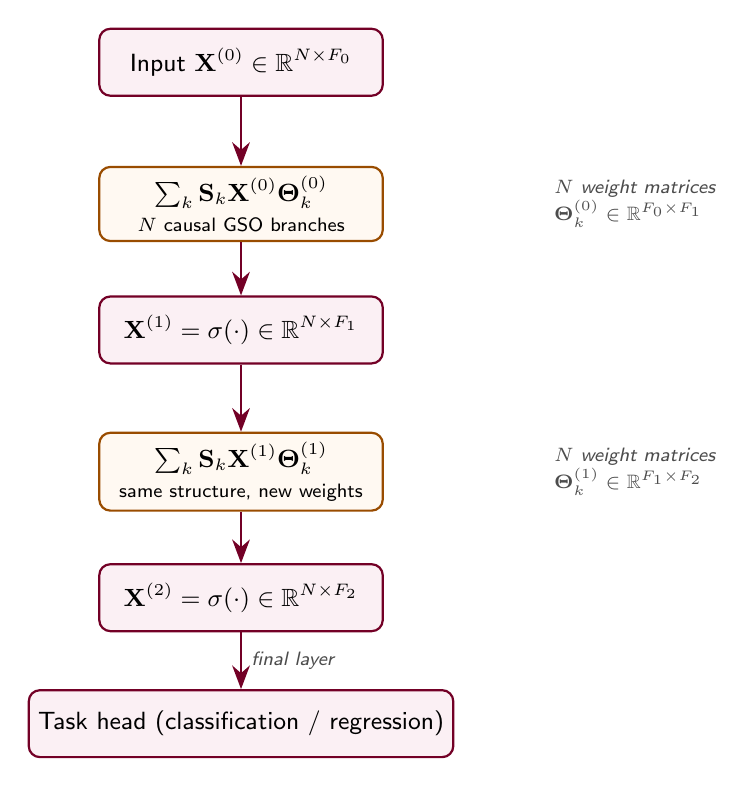
\begin{tikzpicture}[
    box/.style={rectangle, rounded corners=4pt, draw=purple!60!black,
                fill=purple!6!white, thick, minimum width=3.6cm,
                minimum height=0.85cm, font=\small\sffamily, align=center},
    gsobox/.style={rectangle, rounded corners=4pt, draw=orange!60!black,
                   fill=orange!5!white, thick, minimum width=3.6cm,
                   minimum height=0.85cm, font=\small\sffamily, align=center},
    arrow/.style={-{Stealth[length=3mm]}, thick, purple!60!black},
    label/.style={font=\scriptsize\sffamily\itshape, text=gray!60!black}
]
    \node[box]    (inp)  at (0,  0)   {Input $\mathbf{X}^{(0)} \in \mathbb{R}^{N \times F_0}$};
    \node[gsobox] (gso1) at (0, -1.8) {$\sum_{k} \mathbf{S}_k \mathbf{X}^{(0)} \boldsymbol{\Theta}_k^{(0)}$\\{\scriptsize $N$ causal GSO branches}};
    \node[box]    (act1) at (0, -3.4) {$\mathbf{X}^{(1)} = \sigma(\cdot) \in \mathbb{R}^{N \times F_1}$};
    \node[gsobox] (gso2) at (0, -5.2) {$\sum_{k} \mathbf{S}_k \mathbf{X}^{(1)} \boldsymbol{\Theta}_k^{(1)}$\\{\scriptsize same structure, new weights}};
    \node[box]    (act2) at (0, -6.8) {$\mathbf{X}^{(2)} = \sigma(\cdot) \in \mathbb{R}^{N \times F_2}$};
    \node[box]    (out)  at (0, -8.4) {Task head (classification / regression)};

    \draw[arrow] (inp)  -- (gso1);
    \draw[arrow] (gso1) -- (act1);
    \draw[arrow] (act1) -- (gso2);
    \draw[arrow] (gso2) -- (act2);
    \draw[arrow] (act2) -- node[label, right]{final layer} (out);

    % Side annotation
    \node[label, align=left] at (5.0, -1.8)
        {$N$ weight matrices\\$\boldsymbol{\Theta}_k^{(0)} \in \mathbb{R}^{F_0 \times F_1}$};
    \node[label, align=left] at (5.0, -5.2)
        {$N$ weight matrices\\$\boldsymbol{\Theta}_k^{(1)} \in \mathbb{R}^{F_1 \times F_2}$};
\end{tikzpicture}
\caption{The \textbf{Directed Convolutional Network (DCN)} architecture. At each
layer, all $N$ causal GSOs are applied in parallel to the current feature
matrix, each with its own weight matrix. The results are summed and passed
through a pointwise nonlinearity. The total parameter count at layer $\ell$ is
$N \times F_\ell \times F_{\ell+1}$ --- it \emph{scales with the graph size}
$N$.}
\label{fig:dcn_architecture}
\end{figure}

\subsection{Forward Pass: Dimensions and Computation}

Let us trace through the DCN forward pass with concrete dimensions for the gene
network ($N=4$ nodes, $F_0=2$ input features, $F_1=4$ hidden features,
$F_2=1$ output).

\begin{examplebox}{Forward Pass Walkthrough for the Gene Network}

\textbf{Input.} $\mathbf{X}^{(0)} \in \mathbb{R}^{4 \times 2}$: two features
per gene (e.g., expression level and sequence motif score).

\textbf{Layer 0.} For each of the 4 nodes $k \in \{A, B, C, D\}$:
\begin{enumerate}[noitemsep]
    \item Compute $\mathbf{S}_k \mathbf{X}^{(0)} \in \mathbb{R}^{4 \times 2}$
          (apply the $4 \times 4$ causal GSO to the $4 \times 2$ feature matrix).
    \item Multiply by $\boldsymbol{\Theta}_k^{(0)} \in \mathbb{R}^{2 \times 4}$
          to get a $4 \times 4$ contribution.
\end{enumerate}
Sum all 4 contributions: $\sum_k \mathbf{S}_k \mathbf{X}^{(0)} \boldsymbol{\Theta}_k^{(0)}
\in \mathbb{R}^{4 \times 4}$.

Apply ReLU: $\mathbf{X}^{(1)} = \text{ReLU}(\cdot) \in \mathbb{R}^{4 \times 4}$.

\textbf{Layer 1.} Repeat: for each of 4 GSOs, apply to $\mathbf{X}^{(1)} \in
\mathbb{R}^{4 \times 4}$ and multiply by $\boldsymbol{\Theta}_k^{(1)} \in
\mathbb{R}^{4 \times 1}$. Sum, apply ReLU:
$\mathbf{X}^{(2)} \in \mathbb{R}^{4 \times 1}$.

\textbf{Parameter count.} Layer 0: $4 \times 2 \times 4 = 32$ parameters.
Layer 1: $4 \times 4 \times 1 = 16$ parameters. Total: 48 parameters (plus
task head). For a graph of $N$ nodes with $F$ features and $L$ layers, the
total is $O(N F^2 L)$ --- \emph{linear in} $N$.
\end{examplebox}

\subsection{Permutation Equivariance}

The DCN satisfies \textbf{permutation equivariance} (Corollary~1 in the paper):
if we relabel the nodes of the DAG by any permutation $\pi$ that preserves the
DAG structure (i.e., an automorphism), the output is permuted by the same
$\pi$. More precisely, for any topological-order-preserving permutation $\pi$:
\[
    \mathbf{H}(\mathbf{P}_\pi \mathbf{X}) = \mathbf{P}_\pi \mathbf{H}(\mathbf{X})
\]
where $\mathbf{P}_\pi$ is the permutation matrix corresponding to $\pi$. This
is the fundamental equivariance requirement for any respectable graph learning
architecture.

\subsection{DCN-T: The Transposed Variant for Source Detection}

For source detection tasks, information flows in the \emph{opposite} direction
to the DAG's causal edges. We observe who is infected (downstream) and want to
identify the source (upstream). To support backward-looking aggregation, Rey et
al.\ define the \textbf{transposed DCN} (DCN-T) by replacing each causal GSO
$\mathbf{S}_k$ with its transpose $\mathbf{S}_k^\top$:

\begin{equation}
    \mathbf{X}^{(\ell+1)}_{\text{DCN-T}} = \sigma\!\left(
        \sum_{k \in \mathcal{V}} \mathbf{S}_k^\top \, \mathbf{X}^{(\ell)} \,
        \boldsymbol{\Theta}_k^{(\ell)}
    \right)
    \label{eq:dcnt_layer}
\end{equation}

The transposed GSO $\mathbf{S}_k^\top$ aggregates information from a node's
\emph{descendants} rather than its ancestors. For source detection: when we
apply DCN-T to the infection state, each candidate source node's representation
accumulates evidence from all nodes it could have infected (its descendants).
The true source will have the richest set of infected descendants, and DCN-T
is designed to detect exactly this pattern.

\subsection{Computational Complexity}

At each DCN layer, the dominant cost is the $N$ matrix products
$\mathbf{S}_k \mathbf{X}^{(\ell)}$. Each $\mathbf{S}_k$ has at most
$\|\mathbf{S}_k\|_0 \le N^2$ non-zero entries (in practice much fewer for
sparse DAGs). Let $S = \max_k \|\mathbf{S}_k\|_0$ be the maximum sparsity.
The total cost per layer is $O(N \cdot S \cdot F_\ell)$ for the GSO
applications, plus $O(N \cdot F_\ell \cdot F_{\ell+1})$ for the weight
multiplications. On sparse DAGs (e.g., trees or chains), $S = O(N)$, giving
an overall per-layer cost of $O(N^2 F + NF^2)$.

% =============================================================================
\section{Parallel DCN (PDCN) --- Trading Depth for Width}
\label{sec:dagcn_pdcn}
% =============================================================================

The DCN architecture as defined in Equation~(\ref{eq:dcn_layer}) has one
important limitation: its parameter count scales with $N$ (the graph size),
because there are $N$ separate weight matrices $\boldsymbol{\Theta}_k^{(\ell)}$
per layer. For large graphs, this becomes prohibitive. Moreover, the authors
show that the expressiveness gain from stacking multiple DCN layers is limited
by a composition lemma.

\subsection{The Composition Lemma: Depth Does Not Help}

\begin{conceptbox}{Why Deep DCN Has Limited Expressiveness}
\textbf{Lemma (Composition of causal filters).}
The composition of two causal graph filters is itself a causal graph filter.
Formally, if $\mathbf{H}_1 = \mathbf{W}\boldsymbol{\Phi}_1\mathbf{W}^{-1}$ and
$\mathbf{H}_2 = \mathbf{W}\boldsymbol{\Phi}_2\mathbf{W}^{-1}$, then:
\[
    \mathbf{H}_1 \mathbf{H}_2 = \mathbf{W}(\boldsymbol{\Phi}_1\boldsymbol{\Phi}_2)\mathbf{W}^{-1}
\]
which is another causal graph filter with frequency response
$\boldsymbol{\Phi}_1\boldsymbol{\Phi}_2$ (a diagonal matrix, since the product
of two diagonal matrices is diagonal).

\medskip
\textbf{Consequence.} Two DCN layers (ignoring the nonlinearity) collapse into
one DCN layer with a modified frequency response. Adding more layers does not
introduce new representational capabilities that could not be achieved by a
single deeper filter. In the absence of the nonlinearity, a deep linear DCN is
equivalent to a single causal graph filter. The nonlinearity $\sigma$ breaks
this collapse, but only partially: empirically, deep DCN does not offer
substantial gains over a single layer followed by a nonlinearity, and adding
layers primarily increases computational cost without a commensurate accuracy
improvement.
\end{conceptbox}

This motivates a different scaling strategy: rather than going \emph{deep}
(stacking layers), go \emph{wide} (running $N$ parallel branches with shared
weights).

\subsection{The PDCN Architecture}

\begin{mathbox}{Parallel DCN (PDCN)}
The PDCN architecture has $N$ parallel processing branches, one for each causal
GSO. All branches share the same MLP parameters $\boldsymbol{\Theta}^{(\ell)}$:

\begin{equation}
    \mathbf{Z}_k^{(\ell)} = \text{MLP}\!\left(\mathbf{S}_k \mathbf{X}^{(\ell)};
    \boldsymbol{\Theta}^{(\ell)}\right), \quad k \in \mathcal{V}
    \label{eq:pdcn_branch}
\end{equation}

\begin{equation}
    \mathbf{X}^{(\ell+1)} = \sum_{k \in \mathcal{V}} \mathbf{Z}_k^{(\ell)}
    \label{eq:pdcn_sum}
\end{equation}

Each branch applies the same MLP (with ReLU activations and $L$ layers of
hidden dimension $F$) to a different GSO-transformed version of the feature
matrix. The results are summed across all $N$ branches.
\end{mathbox}

\subsection{Architecture Diagram: DCN vs. PDCN}

\begin{figure}[H]
\centering
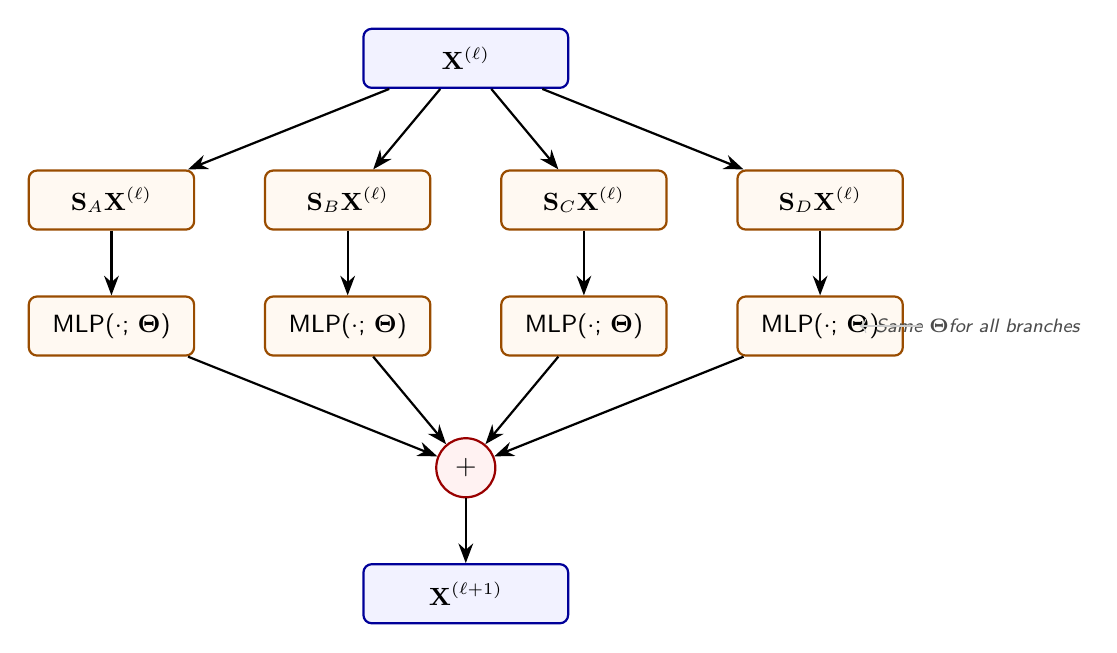
\begin{tikzpicture}[
    inp/.style={rectangle, rounded corners=3pt, draw=blue!60!black,
                fill=blue!5!white, thick, minimum width=2.6cm,
                minimum height=0.75cm, font=\small\sffamily, align=center},
    branch/.style={rectangle, rounded corners=3pt, draw=orange!60!black,
                   fill=orange!5!white, thick, minimum width=2.1cm,
                   minimum height=0.75cm, font=\small\sffamily, align=center},
    sumbox/.style={circle, draw=red!60!black, fill=red!5!white, thick,
                   minimum size=0.75cm, font=\bfseries\sffamily},
    arrow/.style={-{Stealth[length=2.5mm]}, thick},
    label/.style={font=\scriptsize\sffamily\itshape, text=gray!60!black}
]
    % Input
    \node[inp] (X) at (0, 0) {$\mathbf{X}^{(\ell)}$};

    % Four branches (one per GSO)
    \node[branch] (B1) at (-4.5, -1.8) {$\mathbf{S}_A\mathbf{X}^{(\ell)}$};
    \node[branch] (B2) at (-1.5, -1.8) {$\mathbf{S}_B\mathbf{X}^{(\ell)}$};
    \node[branch] (B3) at ( 1.5, -1.8) {$\mathbf{S}_C\mathbf{X}^{(\ell)}$};
    \node[branch] (B4) at ( 4.5, -1.8) {$\mathbf{S}_D\mathbf{X}^{(\ell)}$};

    % MLP boxes (shared weights)
    \node[branch] (M1) at (-4.5, -3.4) {\small MLP($\cdot$; $\boldsymbol{\Theta}$)};
    \node[branch] (M2) at (-1.5, -3.4) {\small MLP($\cdot$; $\boldsymbol{\Theta}$)};
    \node[branch] (M3) at ( 1.5, -3.4) {\small MLP($\cdot$; $\boldsymbol{\Theta}$)};
    \node[branch] (M4) at ( 4.5, -3.4) {\small MLP($\cdot$; $\boldsymbol{\Theta}$)};

    % Sum node
    \node[sumbox] (S) at (0, -5.2) {$+$};

    % Output
    \node[inp] (Xp) at (0, -6.8) {$\mathbf{X}^{(\ell+1)}$};

    % Arrows: input to branches
    \draw[arrow] (X) -- (B1);
    \draw[arrow] (X) -- (B2);
    \draw[arrow] (X) -- (B3);
    \draw[arrow] (X) -- (B4);

    % Arrows: branches to MLPs
    \draw[arrow] (B1) -- (M1);
    \draw[arrow] (B2) -- (M2);
    \draw[arrow] (B3) -- (M3);
    \draw[arrow] (B4) -- (M4);

    % Arrows: MLPs to sum
    \draw[arrow] (M1) -- (S);
    \draw[arrow] (M2) -- (S);
    \draw[arrow] (M3) -- (S);
    \draw[arrow] (M4) -- (S);

    % Sum to output
    \draw[arrow] (S) -- (Xp);

    % Shared weights label
    \node[label] at (6.5, -3.4) {Same $\boldsymbol{\Theta}$\\for all branches};
    \draw[->, gray!40, thin] (5.8, -3.4) -- (5.0, -3.4);
\end{tikzpicture}
\caption{The \textbf{Parallel DCN (PDCN)} architecture for the gene network
($N = 4$). The input $\mathbf{X}^{(\ell)}$ is first transformed by each of the
$N = 4$ causal GSOs in parallel. All $N$ resulting matrices are processed by
the \emph{same} shared MLP (weight-tied across branches), then summed to
produce $\mathbf{X}^{(\ell+1)}$. Parameter count: $O(F^2 L)$ independently
of $N$.}
\label{fig:pdcn_architecture}
\end{figure}

\subsection{Parameter Count: Independent of Graph Size}

The decisive advantage of the PDCN over the DCN is parameter efficiency. In the
DCN, there are $N$ separate weight matrices per layer, giving $O(NF^2L)$ total
parameters. In the PDCN, all $N$ branches share a single MLP, so the total
parameter count is $O(F^2 L)$ --- completely \emph{independent of} $N$.

This has three consequences:

\begin{enumerate}
    \item \textbf{Scalability.} The PDCN can be applied to large DAGs without
          increasing the number of learned parameters. The same model can handle
          DAGs with 10 nodes or 10,000 nodes.
    \item \textbf{Generalisation.} Because weights are shared across branches,
          the PDCN is forced to learn features that are meaningful for any
          GSO-transformed input, not just the one corresponding to a specific
          node $k$. This acts as a form of regularisation.
    \item \textbf{Permutation equivariance (Remark~1).} Sharing weights across
          branches ensures that the PDCN is permutation equivariant: relabelling
          the nodes produces the same output, relabelled identically.
\end{enumerate}

\begin{keyinsight}{PDCN Achieves WL-Expressiveness}
The PDCN can distinguish any pair of non-isomorphic DAGs that differ in their
causal GSO structure. Since the causal GSOs $\{\mathbf{S}_k\}_{k \in
\mathcal{V}}$ uniquely characterise the DAG up to isomorphism (Proposition~2 in
the paper), any function of the full set of GSO-transformed features
$\{\mathbf{S}_k \mathbf{X}\}_{k \in \mathcal{V}}$ is at least as expressive as
the Weisfeiler--Lehman (WL) graph isomorphism test. The PDCN, by processing
each GSO branch with a shared MLP and summing, achieves exactly this level of
expressiveness.
\end{keyinsight}

\subsection{When to Use DCN vs. PDCN}

The choice between DCN and PDCN depends on the specific requirements:

\begin{center}
\begin{tabular}{lll}
\toprule
\textbf{Criterion} & \textbf{DCN} & \textbf{PDCN} \\
\midrule
Parameter count & $O(NF^2L)$ --- scales with $N$ & $O(F^2L)$ --- independent of $N$ \\
Expressiveness & High (per-node weights) & High (WL-level, shared weights) \\
Inductive learning & No (tied to graph size) & Yes (same model, any size) \\
When $N$ is large & Expensive & Preferred \\
When $N$ is small & Both applicable & Preferred for generalisation \\
Source detection & DCN-T (transposed) & PDCN-T (transposed) \\
\bottomrule
\end{tabular}
\end{center}

% =============================================================================
\section{Source Detection with DCN-T}
\label{sec:dagcn_source}
% =============================================================================

The most compelling application of the DAGCN framework in the paper is
\textbf{source identification}: given a signal propagated on a DAG (for example,
a viral cascade on a gene regulatory network), identify the node that initiated
the propagation.

\subsection{The Source Identification Task}

In the source identification setting, we observe the final signal state
$\mathbf{x}_{\text{obs}} \in \mathbb{R}^N$ at every node after the propagation
has run to completion. Under the SEM, this signal was generated as $\mathbf{x}
= \mathbf{W}\mathbf{c}$ where $\mathbf{c}$ has exactly one large non-zero entry
at the source node $k^*$ (and small noise contributions at other nodes). The
task is to identify $k^*$ from $\mathbf{x}_{\text{obs}}$.

\begin{examplebox}{Why This Is Hard}
Suppose the true source is Gene A in our network. Gene A's exogenous
contribution $c_A$ propagates to all its descendants: C and D each accumulate
a contribution of $W_{CA} c_A = c_A$ and $W_{DA} c_A = c_A$ respectively.
The signal at Gene D is $x_D = c_A + c_B + c_C + c_D \approx c_A$ if $c_A$
dominates. But from $x_D$ alone, we cannot tell whether the large signal came
from Gene A or Gene B (both equally contribute to Gene D). We need to look at
the \emph{pattern} across all nodes to identify the source.

In particular, if Gene B's contribution is small ($c_B \approx 0$) but Gene A
is the source ($c_A$ large), then: $x_A = c_A$ (large), $x_B \approx 0$ (small),
$x_C \approx c_A$ (large), $x_D \approx c_A$ (large). The signature is:
large signal at A, C, D; small at B. A model looking only at local node
features or only at direct edges would miss this pattern; it requires reasoning
about the \emph{transitive} influence of Gene A.
\end{examplebox}

\subsection{Why Transposed GSOs Are Needed}

The standard causal GSO $\mathbf{S}_k$ aggregates from a node's \emph{ancestors}
(looking upstream). For source detection, we need the opposite: we need each
candidate source node to aggregate from its \emph{descendants} (looking
downstream). The reason is intuitive --- we want the source node to ``see''
how many and which downstream nodes exhibit the propagated signal.

The transposed GSO $\mathbf{S}_k^\top$ does exactly this. The $(i,j)$ entry of
$\mathbf{S}_k^\top$ is $[\mathbf{S}_k]_{ji}$, which is non-zero when node $i$
is an ancestor of node $j$ and both $j$ and $k$ share a common ancestor. In the
context of source detection, applying $\mathbf{S}_k^\top$ to the observed signal
allows candidate source node $k$ to collect evidence from all nodes downstream
of it:

\[
    [\mathbf{S}_k^\top \mathbf{x}]_i = \sum_{j: i \le j,\; k \le j}
    [\mathbf{W}^\top]_{ij} \, [\mathbf{W}^{-\top}]_{ji} \, x_j
\]

In plain terms: $\mathbf{S}_k^\top$ at node $i$ aggregates the observed signals
of all nodes $j$ that are descendants of both $i$ and $k$. If $i = k^*$ (the
true source), this aggregates evidence from every infected descendant.

\begin{analogybox}{Finding the Source of a Rumour by Asking Who Heard It}
Imagine a rumour that started with one person and spread through a social
network. Each person only passes the rumour to people they directly communicate
with (causal direction: source $\to$ recipients). After the rumour has spread,
you want to find who started it.

You cannot ask who \emph{told} you the rumour (that would be aggregating from
ancestors, looking upstream --- the DCN direction). Instead, you ask each person:
``Of all the people who know the rumour, which ones could only have heard it from
you?'' That question looks \emph{downstream}: it asks who is in your rumour
propagation cone. The person whose downstream cone matches the set of informed
people most precisely is the source. This is exactly what $\mathbf{S}_k^\top$
computes for each candidate source node $k$.
\end{analogybox}

\subsection{Connection to Reversed DAG Approaches}

The DCN-T approach is conceptually aligned with the reversed-DAG message
passing used in the Saram\"{a}ki Temporal Event Graph framework (Chapter~\ref{chap:saramaki}).
Both recognise the same fundamental insight: epidemic source detection is a
\emph{backward inference} problem. The observed infection pattern is the
downstream consequence of the source's action; we must propagate evidence
upstream (in the Saram\"{a}ki approach, by flipping the DAG edges) or equivalently
aggregate from descendants (in the DCN-T approach, by transposing the GSOs).

The key difference is in the representation: the Saram\"{a}ki approach builds
an explicit event-level DAG and reverses it structurally, while the DCN-T works
on the original node-level DAG and reverses the direction of aggregation through
matrix transposition. The underlying causal logic is identical.

\subsection{Experimental Results}

Rey et al.\ evaluate source identification accuracy on synthetic DAGs generated
from Erd\H{o}s--R\'{e}nyi and Barab\'{a}si--Albert DAG models. The source node
generates a large exogenous input $c_{k^*} \gg 0$ and all other nodes have
small noise contributions. The models predict the most likely source node.

The results are striking:

\begin{center}
\begin{tabular}{lcc}
\toprule
\textbf{Model} & \textbf{Accuracy} & \textbf{Notes} \\
\midrule
Standard DCN (forward GSOs) & 0.057 & Near-random; cannot look downstream \\
DCN-T (transposed GSOs) & \textbf{0.997} & Near-perfect; correctly aggregates downstream \\
Standard GCN (undirected) & 0.312 & Partial success; loses causal direction \\
\bottomrule
\end{tabular}
\end{center}

The contrast between standard DCN (0.057 accuracy, essentially random) and
DCN-T (0.997 accuracy, near-perfect) is perhaps the most informative result
in the paper. It is not that the architecture is wrong or the data is
insufficient --- the standard DCN is simply looking in the wrong direction. By
transposing the GSOs, the DCN-T aggregates exactly the right information, and
the task becomes almost trivially easy. The causal direction of aggregation is
not a hyperparameter to be tuned; it is a structural requirement of the task.

The standard GCN achieves 0.312 accuracy --- well above random (0.25 for a
four-class problem) but far below DCN-T. This is because undirected aggregation
captures some of the signal (a node with many infected neighbours is likely
near the source) but corrupts the representation by mixing upstream and
downstream information symmetrically.

% =============================================================================
\section{Summary}
\label{sec:dagcn_summary}
% =============================================================================

This chapter has developed the complete theoretical and practical framework
of Rey, Ajorlou, and Mateos's \textbf{Directed Acyclic Graph Convolutional
Network (DAGCN)}~\cite{rey2025dagcn}. We close with a structured comparison
of the three architectures and a discussion of the paper's position in the
broader landscape.

\subsection{Comparison Table}

\begin{center}
\begin{tabular}{llll}
\toprule
\textbf{Property} & \textbf{Standard GNN} & \textbf{DCN} & \textbf{PDCN} \\
\midrule
Handles DAG structure & No & Yes & Yes \\
Spectral foundation & Eigendecomposition & Transitive closure & Transitive closure \\
Aggregation direction & Both / undirected & Ancestors only & Ancestors only \\
Basis & Eigenvectors of $\mathbf{L}$ & Columns of $\mathbf{W}$ & Columns of $\mathbf{W}$ \\
Shift operators & Powers of $\mathbf{A}$ or $\mathbf{L}$ & $\{\mathbf{S}_k\}_{k \in \mathcal{V}}$ & $\{\mathbf{S}_k\}_{k \in \mathcal{V}}$ \\
Param count / layer & $O(RF^2)$ & $O(NF^2)$ & $O(F^2L)$ \\
Scales with graph & No & Yes (bad) & No (good) \\
Source detection & Poor & Poor (forward) & Excellent (transposed) \\
WL expressiveness & Limited & Yes & Yes \\
Inductive (new graphs) & Limited & No (fixed $N$) & Yes \\
\bottomrule
\end{tabular}
\end{center}

\subsection{The Three Key Contributions}

Rey et al.\ make three tightly coupled contributions:

\begin{enumerate}
    \item \textbf{The causal GSO and DAG Fourier theory.} By recognising the
          transitive closure $\mathbf{W} = (\mathbf{I} - \mathbf{A})^{-1}$ as the
          natural Fourier basis for DAG signals and defining the causal GSOs
          $\mathbf{S}_k = \mathbf{W}\mathbf{D}_k\mathbf{W}^{-1}$, the paper
          provides a rigorous spectral theory for DAGs that avoids the nilpotency
          problem entirely. The spectrum is no longer the (degenerate) eigenvalues
          of $\mathbf{A}$; it is the per-node causal channels, one for each node
          in the graph.

    \item \textbf{The DCN and PDCN architectures.} The DCN generalises the
          causal filter to a deep, multi-feature, nonlinear architecture with
          per-node weight matrices. The PDCN resolves the scaling problem by
          sharing weights across GSO branches, achieving $O(F^2L)$ parameter
          count regardless of graph size. Both architectures are permutation
          equivariant and WL-expressive.

    \item \textbf{The DCN-T transposition for causal inference.} The insight
          that source detection requires \emph{transposed} GSOs --- aggregating
          from descendants rather than ancestors --- is both elegant and
          empirically validated. The accuracy gap between DCN (0.057) and DCN-T
          (0.997) demonstrates that architectural alignment with the task's
          causal direction is not a minor improvement but a categorical difference.
\end{enumerate}

\subsection{Position in the Broader Landscape}

The DAGCN paper occupies a distinctive position in the GNN landscape for
temporal and causal networks. Compared to the approaches studied in previous
chapters:

\paragraph{Versus Saram\"{a}ki's TEG (Chapter~\ref{chap:saramaki}).} Both
approaches recognise that DAG structure is fundamental to causal reasoning on
temporal networks. The TEG approach lifts the problem to the event level,
constructing a new DAG of events and running GNN message passing on it. The
DAGCN approach works directly on the original node-level DAG, using the
transitive closure to build a rich spectral theory. The TEG approach handles
arbitrary temporal networks (including those with undirected contacts), while
DAGCN requires a pre-specified DAG structure.

\paragraph{Versus standard temporal GNNs.} Temporal GNNs such as TGAT or
TGN use attention mechanisms or memory modules to order temporal information,
but they operate on the original node graph and do not exploit DAG structure
explicitly. DAGCN, by contrast, uses the full ancestry structure encoded in
$\mathbf{W}$ to define shift operators. On true DAG data, DAGCN's structural
advantage translates directly into better empirical performance.

\paragraph{Versus backtracking-based methods.} Methods such as the
Backtracking Network of Ru et al.\ use explicit probabilistic likelihood models
to score candidate sources. DAGCN learns these scores end-to-end from data,
without requiring a parametric model of the propagation process. This makes
DAGCN more flexible in settings where the generative model is unknown, at the
cost of requiring labelled training examples of (source, observed signal) pairs.

\begin{keyinsight}{The Central Lesson of This Chapter}
The central lesson of the DAGCN paper is that the appropriate notion of
``graph frequency'' depends fundamentally on the type of graph being processed.
For undirected graphs, the eigenvectors of the Laplacian are the right basis.
For DAGs, the eigenvectors of $\mathbf{A}$ are degenerate and useless; the
right basis is the columns of the transitive closure $\mathbf{W}$. A GNN
designed for undirected graphs cannot simply be applied to a DAG by ignoring
the direction --- it will be blind to the very structure that makes the DAG
informative. The causal GSOs $\{\mathbf{S}_k\}$ provide the first principled,
expressive, and computationally tractable signal processing framework for DAGs,
and the DCN/PDCN architectures operationalise this framework in a learnable,
scalable form.
\end{keyinsight}


% Part V: Experiments \& Evaluation
\part{Experiments \& Evaluation}
\chapter{Experiments, Baselines, and Evaluation}
\label{ch:experiments}

% ============================================================
% CHAPTER INTRODUCTION
% ============================================================

So far we have studied the problem of epidemic source detection and built GNN models to solve it. But how do we know whether a model is \emph{good}? How do we compare two different methods fairly? And how do we actually run the whole pipeline from raw network data to a final number that summarises performance?

This chapter answers all three questions. We begin with the big picture: a tour of the four-stage experiment pipeline. Then we carefully define the evaluation metrics used in this project --- not just their formulas, but their meaning. We examine the \texttt{TSIRData} dataclass that glues everything together, walk through every classical baseline method line by line, and end with practical guidance on running experiments and reading the results.

By the end of this chapter you will be able to:
\begin{itemize}
    \item Run a complete experiment end to end from the command line.
    \item Explain what rank score and top-$k$ score measure, and compute them by hand on a toy example.
    \item Describe what every field in \texttt{TSIRData} stores and why it is shaped the way it is.
    \item Explain why the uniform, degree, and Jordan-center baselines behave the way they do.
    \item Read an experiment results plot and say whether a method is performing well or poorly.
\end{itemize}

% ============================================================
\section{The Experiment Pipeline: Big Picture}
\label{sec:pipeline}
% ============================================================

\begin{conceptbox}{What is a Pipeline?}
A \textbf{pipeline} is a sequence of steps where the output of each step becomes the input to the next. In software engineering, pipelines are used when a computation is too large or too complex to run as a single monolithic script. Each step can be debugged, rerun, and compared independently.

Our experiment pipeline has four stages:
\begin{enumerate}
    \item \textbf{Simulate} --- generate epidemic data using the SIR model on a network.
    \item \textbf{Infer} --- run inference methods (GNN or classical baseline) to identify the source.
    \item \textbf{Evaluate} --- score every method using standardised metrics.
    \item \textbf{Visualise} --- produce plots to understand the results.
\end{enumerate}
\end{conceptbox}

\subsection{Pipeline Diagram}

The following diagram illustrates the full data flow from raw network files to final plots.

\begin{figure}[h!]
\centering
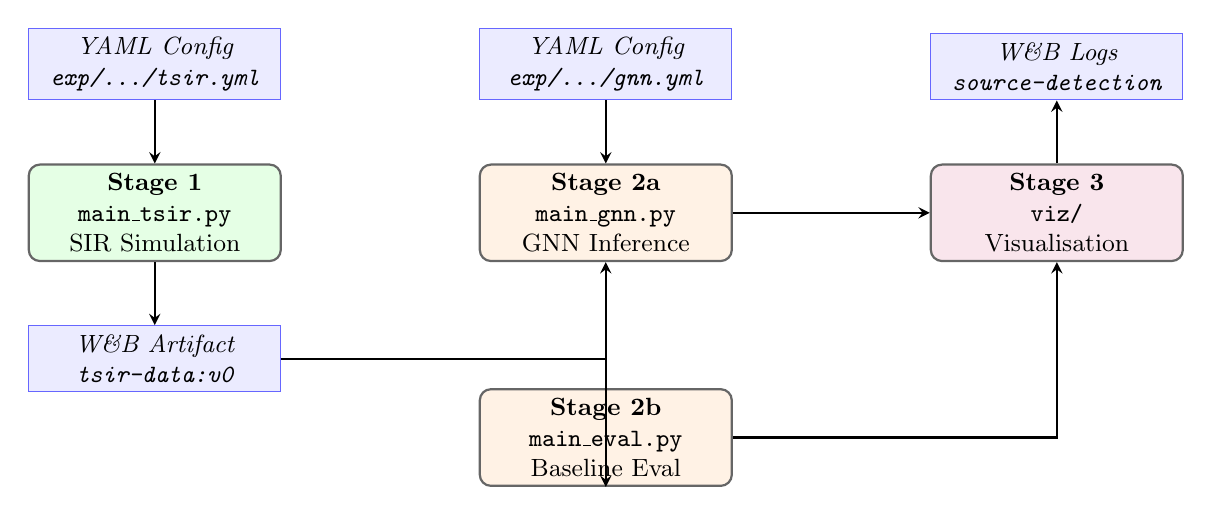
\begin{tikzpicture}[
    node distance = 1.5cm and 2.5cm,
    box/.style     = {rectangle, rounded corners, draw=black!60, fill=white,
                      minimum width=3.2cm, minimum height=1.0cm,
                      font=\small, align=center, thick},
    artifact/.style= {rectangle, draw=blue!60, fill=blue!8,
                      minimum width=3.2cm, minimum height=0.8cm,
                      font=\small\itshape, align=center},
    arrow/.style   = {->, >=stealth, thick},
    label/.style   = {font=\scriptsize\ttfamily, align=center}
]

% Stage 1
\node[box, fill=green!10]  (tsir)   {\textbf{Stage 1}\\
                                      \texttt{main\_tsir.py}\\
                                      SIR Simulation};
\node[artifact, below=0.8cm of tsir] (art1) {W\&B Artifact\\
                                               \texttt{tsir-data:v0}};

% Stage 2a
\node[box, fill=orange!10, right=2.5cm of tsir] (gnn)  {\textbf{Stage 2a}\\
                                                          \texttt{main\_gnn.py}\\
                                                          GNN Inference};

% Stage 2b
\node[box, fill=orange!10, below=1.6cm of gnn]  (eval) {\textbf{Stage 2b}\\
                                                          \texttt{main\_eval.py}\\
                                                          Baseline Eval};

% Stage 3
\node[box, fill=purple!10, right=2.5cm of gnn] (viz)  {\textbf{Stage 3}\\
                                                         \texttt{viz/}\\
                                                         Visualisation};

% YAML configs
\node[artifact, above=0.8cm of tsir]  (cfg1) {YAML Config\\
                                               \texttt{exp/.../tsir.yml}};
\node[artifact, above=0.8cm of gnn]   (cfg2) {YAML Config\\
                                               \texttt{exp/.../gnn.yml}};
\node[artifact, above=0.8cm of viz]   (cfg3) {W\&B Logs\\
                                               \texttt{source-detection}};

% Arrows
\draw[arrow] (cfg1) -- (tsir);
\draw[arrow] (tsir) -- (art1);
\draw[arrow] (art1.east) -| (gnn.south);
\draw[arrow] (art1.east) -| (eval.south);
\draw[arrow] (cfg2) -- (gnn);
\draw[arrow] (gnn)  -- (viz);
\draw[arrow] (eval) -| (viz.south);
\draw[arrow] (viz)  -- (cfg3);

\end{tikzpicture}
\caption{The four-stage experiment pipeline. Stage 1 produces a versioned data artifact; Stages 2a and 2b both consume it independently; Stage 3 collects all results from W\&B and produces comparison plots.}
\label{fig:pipeline}
\end{figure}

\subsection{Stage 1: Generating Ground-Truth Data (\texttt{main\_tsir.py})}

The first stage runs SIR simulations on a temporal network and saves everything to disk. It produces three types of data:

\begin{itemize}
    \item \textbf{Ground-truth simulations} (\texttt{ground\_truth\_\{S,I,R\}.bin}): For every possible source node $v_0 \in \{0, \ldots, N-1\}$, we run the SIR model $n\_\text{runs}$ times. The final state of every node (Susceptible, Infected, or Recovered) is recorded. This is the labelled dataset used for evaluation.

    \item \textbf{Monte Carlo simulations} (\texttt{monte\_carlo\_\{S,I,R\}.bin}): Also from every source, but $mc\_\text{runs}$ independent realisations. This data is given to the GNN as \emph{training features} --- the model can look at Monte Carlo simulations to understand what outbreaks from a given source tend to look like.

    \item \textbf{Maximal-outbreak simulations} (\texttt{maximal\_outbreak\_S.bin}): Run with $\beta=1$, $\mu=0$, so the infection spreads deterministically to every reachable node. This maps out the \emph{maximum possible spread} from each source, used to build the \texttt{possible} mask (see Section~\ref{sec:tsirdata}).
\end{itemize}

\begin{codewalk}{Reading \texttt{main\_tsir.py} Step by Step}
\begin{lstlisting}[language=Python]
# Step 1: Load config and set up W&B tracking
cfg = setup_tsir_run(args.cfg)
local_folder = f"data/{wandb.run.id}"

# Step 2: Load the temporal network from file
H = load_network(cfg)
n_nodes = H.number_of_nodes()

# Step 3: Convert network to a C-readable format
H_cread = make_c_readable_from_networkx(H, t_max=cfg.nwk.t_max)

# Step 4: Run ground-truth SIR (n_nodes sources x n_runs each)
truth_S, truth_I, truth_R = sir_ground_truth(cfg, H_cread, n_nodes)

# Step 5: Run Monte Carlo SIR (training data for GNN)
sir_monte_carlo(cfg, H_cread, n_nodes, local_folder)

# Step 6: Maximal outbreak (beta=1, mu=0) for the 'possible' mask
sir_maximal_outbreak(cfg, H_cread, n_nodes, local_folder)

# Step 7: Build and save the 'possible' mask
# possible[s, r, v] = 1 iff node v was NOT susceptible in run r from source s
truth_S_3d = truth_S.reshape(n_nodes, cfg.sir.n_runs, n_nodes)
possible   = (1 - truth_S_3d).astype(np.int8)

# Step 8: Log everything as a versioned W&B artifact
artifact = wandb.Artifact(name=args.data, type="tsir-data")
artifact.add_dir(local_folder)
wandb.log_artifact(artifact)
\end{lstlisting}
\textbf{Key idea:} The \texttt{possible} mask is built from the ground-truth runs. A node that stayed Susceptible in \emph{every} run from source $s$ is very unlikely to be the true source --- it was never infected. The mask eliminates such impossible candidates, which makes inference much more tractable.
\end{codewalk}

\subsection{Stage 2a: GNN Inference (\texttt{main\_gnn.py})}

The GNN training script loads the W\&B artifact produced in Stage 1, builds the Monte Carlo data into input feature tensors $X$, trains a \texttt{StaticGNN}, and records evaluation scores. We cover the GNN architecture in detail in earlier chapters; here we focus on the evaluation interface.

After training, the script runs inference on the \emph{ground-truth} observations (not the Monte Carlo training data) and calls the same scoring functions as the baseline evaluator:

\begin{lstlisting}[language=Python]
gnn_log_lik = results.cpu().numpy() - lik_possible
gnn_ranks   = compute_ranks(gnn_log_lik, n_nodes=data.n_nodes, n_runs=n_truth)
top_k_score(gnn_ranks, sel, k)
rank_score(gnn_ranks, sel, offset)
\end{lstlisting}

\subsection{Stage 2b: Classical Baseline Evaluation (\texttt{main\_eval.py})}

This script evaluates all non-learning baselines on the same artifact. It uses the exact same scoring functions, ensuring a fair, apples-to-apples comparison. The baselines available are:

\begin{center}
\begin{tabular}{lll}
\toprule
\textbf{Baseline}     & \textbf{Signal Used}                   & \textbf{Cost}    \\
\midrule
\texttt{uniform}      & None (equal probability to all nodes)  & $O(N)$           \\
\texttt{random}       & None (random pick from possible set)   & $O(N)$           \\
\texttt{degree}       & Degree in infected subgraph            & $O(N + E)$       \\
\texttt{closeness}    & Closeness centrality in infected subgraph & $O(N^2)$      \\
\texttt{betweenness}  & Betweenness centrality in infected subgraph & $O(N^3)$    \\
\texttt{jordan\_center} & Minimum eccentricity in infected subgraph & $O(N^2)$    \\
\bottomrule
\end{tabular}
\end{center}

\subsection{Stage 3: Visualisation (\texttt{viz/})}

The visualisation scripts query the W\&B API to collect metric summaries from all completed runs (both GNN runs and baseline runs) and produce comparison plots. Results for different methods are identified by the W\&B tags and job types attached to each run.

% ============================================================
\section{Evaluation Metrics: From Scratch}
\label{sec:metrics}
% ============================================================

\begin{conceptbox}{The Core Question}
Every evaluation metric in this project ultimately answers one question: \textbf{how quickly can a method lead us to the true source?}

Think of it like a police investigation. We have $N$ suspects. After running our inference method, we sort all suspects from most likely to least likely. We then check how far down the list the true culprit appears.
\begin{itemize}
    \item If the true source is \textbf{rank 1} (top of the list) --- perfect. We found them immediately.
    \item If the true source is \textbf{rank $N$} (bottom of the list) --- the method is actively misleading.
    \item A \textbf{random guesser} would, on average, place the true source at rank $N/2$.
\end{itemize}
Every metric below is a different way to summarise this rank.
\end{conceptbox}

\subsection{Computing the Rank}

Before defining any metric, we need to define what a ``rank'' is. The code in \texttt{eval/ranks.py} computes it as follows.

\begin{codewalk}{Computing Ranks (\texttt{eval/ranks.py})}
\begin{lstlisting}[language=Python]
def compute_ranks(values, n_nodes, n_runs):
    # 'values' is a matrix of shape [n_nodes * n_runs, n_nodes]
    # values[i, j] = score assigned to node j as source for observation i

    # Step 1: for each observation i, find the score assigned to the TRUE source
    # The true source for observation i = (i // n_runs)
    source_values = values[
        np.arange(n_nodes * n_runs),
        np.repeat(np.arange(n_nodes), n_runs)
    ]

    # Step 2: rank = number of nodes with a HIGHER score than the true source
    # rank=0 means the true source has the highest score (it is #1)
    rank = np.sum(values > source_values[:, None], axis=1)

    # Step 3: handle ties by breaking them randomly
    ties = np.sum(values == source_values[:, None], axis=1)
    rank = rank + np.random.randint(ties) + 1

    return rank  # rank[i] is in {1, 2, ..., N}
\end{lstlisting}
\textbf{Note on indexing:} The matrix \texttt{values} has $N \times n\_\text{runs}$ rows, one for each (source, run) pair. The true source for row $i$ is $\lfloor i / n\_\text{runs} \rfloor$. The code uses \texttt{np.repeat} to build this index array efficiently.
\end{codewalk}

\begin{examplebox}{Rank Computation by Hand}
Suppose $N = 5$ nodes and we are evaluating one observation (source = node 2). The method assigns these scores:

\begin{center}
\begin{tabular}{ccccc}
\toprule
Node 0 & Node 1 & \textbf{Node 2 (true)} & Node 3 & Node 4 \\
\midrule
0.10   & 0.05   & \textbf{0.60}           & 0.20   & 0.05   \\
\bottomrule
\end{tabular}
\end{center}

How many nodes have a score \emph{strictly greater} than 0.60? None. So $\text{rank} = 0 + 1 = 1$.

Now a bad case: the true source (node 2) gets score 0.01, and all others get higher scores. Then rank $= 4 + 1 = 5$.

A random baseline: each node gets roughly the same score, so the true source ends up at rank $\approx N/2 \approx 2.5$ on average.
\end{examplebox}

\subsection{Rank Score}

\begin{mathbox}{Rank Score Definition}
For a single observation with true source rank $r$ out of $N$ nodes, the \textbf{rank score} is:

\[
\text{RS}(r) = \frac{1+\delta}{r+\delta}
\]

where $\delta \geq 0$ is an offset parameter (called \texttt{inverse\_rank\_offset} in the config). When $\delta = 0$, this simplifies to $1/r$.

For $\delta = 0$:
\begin{itemize}
    \item If rank = 1 (perfect): $\text{RS} = 1/1 = 1.0$
    \item If rank = 2: $\text{RS} = 1/2 = 0.5$
    \item If rank = $N$ (worst): $\text{RS} = 1/N \approx 0$
\end{itemize}

The \textbf{mean rank score} over a dataset of $Q$ test cases is:
\[
\overline{\text{RS}} = \frac{1}{Q} \sum_{q=1}^{Q} \frac{1+\delta}{r_q + \delta}
\]

A random baseline achieves $\overline{\text{RS}} \approx \frac{2}{N+1}$ in expectation. A perfect method achieves $\overline{\text{RS}} = 1.0$.
\end{mathbox}

\begin{codewalk}{Rank Score in Code (\texttt{eval/scores.py})}
\begin{lstlisting}[language=Python]
def rank_score(ranks, sel, offset=0):
    # ranks: array of rank values for each (source, run) pair
    # sel:   boolean mask --- only count "valid" outbreaks
    # offset: the delta parameter above
    return np.mean((1 + offset) / (ranks[sel] + offset))
\end{lstlisting}
The \texttt{sel} mask filters out degenerate outbreaks where too few nodes were infected (controlled by \texttt{min\_outbreak} in the eval config). Evaluating on tiny outbreaks would be unfair because even random methods might get lucky.
\end{codewalk}

\begin{analogybox}{Why Use $1/r$ Instead of $r/N$?}
You might expect the metric to be $r/N$ (normalised rank), where lower is better. The project uses $1/r$ (reciprocal rank), where \textbf{higher is better}. Why?

The reciprocal rank rewards being ``close to the top'' much more generously. Consider two methods:
\begin{itemize}
    \item Method A: True source is always at rank 1. Score = 1.0. Perfect.
    \item Method B: True source is always at rank 2. Score = 0.5. Still quite good.
    \item Method C: True source is always at rank 50 (out of 100). Score = 0.02. Poor.
\end{itemize}

With normalised rank $r/N$, Methods B and C look equidistant from Method A. With reciprocal rank, Method B is recognised as much better than C. This matches the epidemiological use case: getting the source in the top 3 is operationally useful; getting it at rank 50 is not.
\end{analogybox}

\subsection{Top-$k$ Score}

\begin{mathbox}{Top-$k$ Score Definition}
The \textbf{top-$k$ score} is a binary metric. For each test case, it asks: is the true source among the $k$ highest-ranked nodes?

\[
\text{Top}_k(r) = \mathbf{1}[r \leq k]
\]

The mean top-$k$ score over $Q$ test cases is:
\[
\overline{\text{Top}_k} = \frac{1}{Q} \sum_{q=1}^{Q} \mathbf{1}[r_q \leq k]
\]

This is simply the fraction of test cases where the source is in the top-$k$ predictions.
\end{mathbox}

\begin{codewalk}{Top-$k$ Score in Code (\texttt{eval/scores.py})}
\begin{lstlisting}[language=Python]
def top_k_score(ranks, sel, k=5):
    # Returns the fraction of valid outbreaks where the true source
    # was ranked in the top k
    return np.mean(ranks[sel] <= k)
\end{lstlisting}
\end{codewalk}

\begin{examplebox}{Top-$k$ Score Concrete Example}
Network has $N = 100$ nodes. We evaluate over 1000 test cases. A method produces:
\begin{itemize}
    \item 420 cases where the true source is rank 1 (top-1 = 42\%)
    \item 180 more cases where it is rank 2, 3, 4, or 5
    \item Total: 600 cases where the source is in the top 5 (top-5 = 60\%)
\end{itemize}

For a \textbf{random baseline} on $N=100$ nodes:
\begin{itemize}
    \item Expected top-1 score: $1/100 = 1\%$
    \item Expected top-5 score: $5/100 = 5\%$
\end{itemize}

So a method that achieves 60\% top-5 is \emph{twelve times better} than random at finding the source within 5 guesses. This is a dramatic improvement and corresponds to real operational utility.
\end{examplebox}

\subsection{The \texttt{sel} Mask: Filtering Valid Outbreaks}

Not every simulation is worth evaluating. If only one or two nodes get infected, the source detection problem is trivially easy (or trivially ambiguous). The \texttt{min\_outbreak} threshold filters these out:

\begin{lstlisting}[language=Python]
# sel[i] = True if observation i has at least min_outbreak non-susceptible nodes
sel = (1 - truth_S_flat).sum(axis=1) >= eval_cfg["min_outbreak"]
\end{lstlisting}

In the toy Holme network config, \texttt{min\_outbreak: 2} means we only evaluate outbreaks where at least 2 nodes were infected or recovered.

\subsection{Other Metrics in the Codebase}

The \texttt{eval/scores.py} module also defines several additional metrics that may be used for deeper analysis:

\begin{itemize}
    \item \textbf{Normalised Brier Score}: Measures the calibration of the predicted probability distribution. A well-calibrated method not only ranks the true source highly, but also assigns realistic confidence values. Defined as:
    \[
    \text{NBS} = \frac{1}{Q} \sum_{q} \frac{\sum_v (x_v^* - \hat{p}_v)^2}{2/N}
    \]
    where $x_v^* \in \{0,1\}$ is the true source indicator and $\hat{p}_v$ is the predicted probability. Normalised by $2/N$ (the score of a uniform predictor).

    \item \textbf{Normalised Entropy}: Measures how ``spread out'' the predicted distribution is. A sharp, confident prediction has low entropy. A confused, nearly-uniform prediction has high entropy close to 1.

    \item \textbf{Credible Set Coverage}: The smallest set of top-ranked nodes that captures at least probability mass $p$. Reports whether the true source falls within this credible set.
\end{itemize}

% ============================================================
\section{The \texttt{TSIRData} Dataclass}
\label{sec:tsirdata}
% ============================================================

\begin{conceptbox}{Why a Dataclass?}
Loading the simulation data from binary files involves many steps: resolving the W\&B artifact, reading flat binary arrays, reshaping them to the correct 3D tensors, and building derived quantities like the \texttt{possible} mask. Wrapping all of this in a single \texttt{dataclass} means every subsequent script (GNN training, baseline evaluation, visualisation) gets the same clean interface regardless of where the data lives.
\end{conceptbox}

\subsection{Fields and Shapes}

\begin{codewalk}{\texttt{TSIRData} Dataclass (\texttt{setup/data\_loader.py})}
\begin{lstlisting}[language=Python]
@dataclass
class TSIRData:
    config:           dict          # original YAML config from the TSIR run
    n_nodes:          int           # N = number of nodes in the network
    n_runs:           int           # number of ground-truth runs per source
    mc_runs:          int           # number of Monte Carlo runs per source
    mc_S:             np.ndarray    # shape: (N, mc_runs, N)
    mc_I:             np.ndarray    # shape: (N, mc_runs, N)
    mc_R:             np.ndarray    # shape: (N, mc_runs, N)
    truth_S:          np.ndarray    # shape: (N, n_runs, N)
    truth_I:          np.ndarray    # shape: (N, n_runs, N)
    truth_R:          np.ndarray    # shape: (N, n_runs, N)
    maximal_outbreak: np.ndarray    # shape: (N, N) -- fraction ever infected
    possible:         np.ndarray    # shape: (N, n_runs, N) -- int8 mask
    lik_possible:     np.ndarray    # shape: (N, n_runs, N) -- log-prior mask
\end{lstlisting}
\end{codewalk}

\subsection{Understanding the 3D Tensor Shape}

The shape \texttt{(N, n\_runs, N)} appears repeatedly and deserves careful explanation.

\begin{examplebox}{Decoding the Shape \texttt{(N, n\_runs, N)}}
Let $N = 100$ nodes and $n\_\text{runs} = 5000$. The array \texttt{truth\_I} has shape \texttt{(100, 5000, 100)}.

The three axes are:
\begin{enumerate}
    \item \textbf{Axis 0 --- source node} ($s \in \{0, \ldots, 99\}$): Which node was the epidemic source?
    \item \textbf{Axis 1 --- run index} ($r \in \{0, \ldots, 4999\}$): Which of the 5000 independent realisations?
    \item \textbf{Axis 2 --- observation node} ($v \in \{0, \ldots, 99\}$): What was the state of node $v$?
\end{enumerate}

So \texttt{truth\_I[5, 2, 8] = 1} means:
\begin{quote}
``In the epidemic that started at node 5, in the 3rd realisation (0-indexed), node 8 was \textbf{Infected} at the observation time.''
\end{quote}

Similarly, \texttt{truth\_S[5, 2, 8] = 1} means node 8 was \textbf{Susceptible} (never infected), and \texttt{truth\_R[5, 2, 8] = 1} means node 8 had \textbf{Recovered}.

Note: exactly one of \texttt{truth\_S}, \texttt{truth\_I}, \texttt{truth\_R} equals 1 for any given \texttt{(s, r, v)} triple. They form a one-hot encoding of the SIR state.
\end{examplebox}

\subsection{The \texttt{possible} Mask}

\begin{conceptbox}{Why Do We Need a \texttt{possible} Mask?}
Not every node is a plausible epidemic source for every observation. If node 42 was never infected in any of the observed runs, it is extremely unlikely to have been the origin. Including it as a candidate would only dilute the probability mass assigned to genuinely plausible sources.

The \texttt{possible} mask is a binary array:
\[
\texttt{possible}[s, r, v] = \begin{cases}
1 & \text{if node } v \text{ was Infected or Recovered in run } r \text{ from source } s \\
0 & \text{if node } v \text{ was Susceptible throughout}
\end{cases}
\]

In source-detection terms: ``For observation $(s, r)$, which nodes are feasible source candidates?'' Only infected or recovered nodes can have been the source --- a Susceptible node provably was not infected, so it could not have started the outbreak.
\end{conceptbox}

\begin{codewalk}{How \texttt{possible} is Built (\texttt{main\_tsir.py})}
\begin{lstlisting}[language=Python]
truth_S_3d = truth_S.reshape(n_nodes, cfg.sir.n_runs, n_nodes)
# possible[s, r, v] = 1 if node v was NOT Susceptible in run r from source s
possible = (1 - truth_S_3d).astype(np.int8)
possible.tofile(f"{local_folder}/possible_sources.bin")
\end{lstlisting}
\textbf{Key arithmetic:} The SIR state is stored as three separate arrays. \texttt{truth\_S[s, r, v] = 1} means Susceptible. Subtracting from 1 flips this: \texttt{(1 - truth\_S)[s, r, v] = 1} means ``was infected or recovered at some point,'' i.e., is a valid candidate.
\end{codewalk}

\subsection{The \texttt{lik\_possible} Log-Prior}

\begin{mathbox}{Log-Prior for Impossible Nodes}
When we compute log-likelihoods to rank source candidates, we need to ensure that impossible candidates are assigned probability zero. The \texttt{lik\_possible} field achieves this via an additive correction in log-space:

\[
\texttt{lik\_possible}[s, r, v] = \begin{cases}
0 & \text{if node } v \text{ is a possible source for } (s, r) \\
+\infty & \text{if node } v \text{ is impossible}
\end{cases}
\]

Adding this to a log-likelihood vector (with sign convention log-lik $-$ lik\_possible) sets impossible nodes to $-\infty$, driving their softmax probability to zero.

In the code:
\begin{lstlisting}[language=Python]
lik_possible = np.where(possible == 1, 0, np.inf)
\end{lstlisting}
Then in inference:
\begin{lstlisting}[language=Python]
log_probs_corrected = model_log_probs - lik_possible
# Impossible nodes now have -inf log-probability
\end{lstlisting}
\end{mathbox}

\subsection{The \texttt{maximal\_outbreak} Array}

The \texttt{maximal\_outbreak} array records, for each source node, the set of nodes that \emph{could ever} be reached if $\beta = 1$ and $\mu = 0$ (infection spreads to every contact, recovery never happens). This gives the upper bound on the set of infected nodes.

Shape: \texttt{(N, N)}. Entry \texttt{maximal\_outbreak[s, v] = 1} means node $v$ is reachable from source $s$ through the temporal contact sequence.

% ============================================================
\section{Classical Baselines: Code Walkthroughs}
\label{sec:baselines}
% ============================================================

Classical baselines are methods that do not require any training. They use simple heuristics --- either ignoring the network structure entirely or using only the static graph topology --- to rank candidate source nodes. They are valuable for two reasons:

\begin{enumerate}
    \item \textbf{Lower bounds on performance}: Any serious inference method must beat these.
    \item \textbf{Insight into what information matters}: A baseline that does surprisingly well tells us that the corresponding signal (e.g., node degree) is informative for source detection.
\end{enumerate}

\subsection{Uniform Baseline}

\begin{conceptbox}{Uniform Baseline: The ``Know Nothing'' Estimator}
The uniform baseline assigns equal probability to every possible source candidate. It uses zero information from the observed epidemic.
\end{conceptbox}

\begin{codewalk}{Uniform Baseline (\texttt{main\_eval.py})}
\begin{lstlisting}[language=Python]
if baseline == "uniform":
    u = poss.astype(np.float32)   # 1 for possible sources, 0 otherwise
    s = u.sum()                    # total number of possible sources
    probs[flat_idx] = u / s if s > 0 else np.ones(n_nodes) / n_nodes
    continue
\end{lstlisting}
\textbf{Line by line:}
\begin{itemize}
    \item \texttt{poss} is the binary \texttt{possible} vector for this specific observation.
    \item We convert it to float and normalise: each possible node gets probability $1 / |\mathcal{P}|$ where $\mathcal{P}$ is the set of possible nodes.
    \item The fallback (\texttt{else} branch) handles the pathological case where no node was infected at all.
\end{itemize}
\textbf{Expected performance:} The expected rank of the true source is $|\mathcal{P}|/2$. Since $|\mathcal{P}| \approx N$ for large outbreaks, the expected rank score is approximately $2/(N+1) \approx 2/N$ for large $N$.
\end{codewalk}

\subsection{Random Baseline}

\begin{codewalk}{Random Baseline (\texttt{main\_eval.py})}
\begin{lstlisting}[language=Python]
if baseline == "random":
    u = poss.astype(np.float32)
    s = u.sum()
    p = u / s if s > 0 else np.ones(n_nodes) / n_nodes
    chosen = int(np.random.choice(n_nodes, p=p))
    probs[flat_idx, chosen] = 1.0   # put ALL probability on one random node
    continue
\end{lstlisting}
Unlike the uniform baseline (which spreads probability uniformly), the random baseline \emph{commits} to a single random guess. The entire probability mass 1.0 goes to one randomly-chosen node.

\textbf{When are they different?} For rank score, uniform and random baselines have the same expected performance (both are random). For top-1 accuracy, uniform gives $1/|\mathcal{P}|$ while random gives the same. They differ in Brier score: uniform has lower Brier score because it doesn't waste all mass on a single wrong guess.
\end{codewalk}

\subsection{Degree Baseline}

\begin{conceptbox}{Degree Baseline: The ``Super-Spreader'' Heuristic}
The degree baseline uses the intuition that highly connected nodes are more likely to be epidemic sources because they can infect more neighbours and thus cause larger outbreaks.

Importantly, it computes degree within the \emph{infected subgraph} --- only considering edges among nodes that were observed to be infected or recovered. This avoids confusing global network hubs with local epidemic centres.
\end{conceptbox}

\begin{codewalk}{Degree Baseline (\texttt{main\_eval.py})}
\begin{lstlisting}[language=Python]
# First, build the infected subgraph from the static network
def _infected_subgraph(H_static, I_snap, R_snap):
    # Find all nodes that were Infected OR Recovered
    infected_nodes = list(np.where((I_snap + R_snap) > 0)[0])
    if not infected_nodes:
        return nx.Graph()
    # Return only the subgraph induced by these nodes
    return H_static.subgraph(infected_nodes).copy()

# Then, for the degree baseline:
G_sub = _infected_subgraph(H_static, I_snap, R_snap)

if baseline == "degree":
    # Degree of each node within the infected subgraph
    scores_dict = {n: float(d) for n, d in G_sub.degree()}
\end{lstlisting}
\textbf{Key insight:} Using the infected subgraph is critical. The source node is by definition part of the infected subgraph, and its local neighbourhood within that subgraph reflects how the epidemic actually spread. A node at the ``hub'' of the infected region is geometrically central.

\textbf{Limitation:} This heuristic works well in networks where sources tend to be high-degree nodes (e.g., Barab{\'a}si-Albert scale-free networks). In random networks where all nodes have similar degrees, it provides little signal.
\end{codewalk}

\subsection{Jordan Center Baseline}

\begin{conceptbox}{Jordan Center: The Geometric Centre of the Epidemic}
The Jordan center of a graph is the node that minimises its \emph{eccentricity} --- the maximum shortest-path distance to any other node in the graph.

Intuitively: if an epidemic spreads outward from a source at roughly uniform speed in all topological directions, the infected region will look like a ``ball'' centred on the source node. The Jordan center is the algorithm's best guess for the centre of this ball.
\end{conceptbox}

\begin{mathbox}{Eccentricity and Jordan Center}
Let $G_I = (\mathcal{V}_I, \mathcal{E}_I)$ be the infected subgraph. For each node $v \in \mathcal{V}_I$, define its \textbf{eccentricity}:

\[
\varepsilon(v) = \max_{u \in \mathcal{V}_I} d(v, u)
\]

where $d(v, u)$ is the shortest-path distance between $v$ and $u$ in $G_I$.

The \textbf{Jordan center} is:
\[
v^* = \arg\min_{v \in \mathcal{V}_I} \varepsilon(v)
\]

The scoring converts eccentricity into a score (so that higher score = more likely source):
\[
\text{score}(v) = \varepsilon_{\max} + 1 - \varepsilon(v)
\]

where $\varepsilon_{\max} = \max_v \varepsilon(v)$ is the maximum eccentricity in the subgraph.
\end{mathbox}

\begin{codewalk}{Jordan Center Baseline (\texttt{main\_eval.py})}
\begin{lstlisting}[language=Python]
elif baseline == "jordan_center":
    # Handle disconnected infected subgraph: use only the largest component
    if not nx.is_connected(G_sub):
        G_cc = G_sub.subgraph(
            max(nx.connected_components(G_sub), key=len)
        ).copy()
    else:
        G_cc = G_sub

    # Compute eccentricity for every node in the component
    ecc = nx.eccentricity(G_cc)

    # Convert to score: lower eccentricity -> higher score
    max_ecc = max(ecc.values()) + 1
    scores_dict = {n: float(max_ecc - e) for n, e in ecc.items()}
\end{lstlisting}
\textbf{The disconnected-component handling} is important. In practice, the infected subgraph may not be connected: perhaps two separate clusters were infected in the same observation window, or the network itself has bridge nodes. Eccentricity is only well-defined within a connected graph, so we take the largest connected component.

\textbf{When Jordan Center fails:} The method assumes spatially uniform spread speed. In temporal networks, a contact that happens early in time can ``teleport'' the infection to a distant node. The Jordan center in the static topology may be far from the temporal propagation centre.
\end{codewalk}

\subsection{From Scores to Probabilities: The \texttt{\_scores\_to\_probs} Function}

All topology-based baselines produce a dictionary of \texttt{\{node: score\}} pairs covering only the infected subgraph. The helper function \texttt{\_scores\_to\_probs} converts this into a full probability vector over all $N$ nodes, respecting the \texttt{possible} mask:

\begin{codewalk}{Score-to-Probability Conversion (\texttt{main\_eval.py})}
\begin{lstlisting}[language=Python]
def _scores_to_probs(scores, n_nodes, poss):
    # Step 1: fill in scores for nodes in the infected subgraph
    vec = np.zeros(n_nodes, dtype=np.float64)
    for node, score in scores.items():
        if 0 <= node < n_nodes:
            vec[node] = max(0.0, score)

    # Step 2: zero out impossible nodes (those outside 'possible' mask)
    vec = vec * poss.astype(np.float64)

    # Step 3: normalise to a valid probability distribution
    total = vec.sum()
    if total > 0:
        return (vec / total).astype(np.float32)

    # Fallback: uniform over possible nodes
    u = poss.astype(np.float64)
    s = u.sum()
    return (u / s if s > 0 else np.ones(n_nodes) / n_nodes).astype(np.float32)
\end{lstlisting}
\end{codewalk}

\begin{keyinsight}{Why Multiply by \texttt{possible}?}
The \texttt{possible} mask ensures that nodes which were never infected in the observation are assigned zero probability mass. Even if the degree baseline assigns a high score to a node that happened to be Susceptible in this particular run, that score is discarded. This is the correct Bayesian thing to do: if we \emph{observe} that node $v$ was Susceptible throughout, then $v$ provably was not the source.
\end{keyinsight}

% ============================================================
\section{Running an Experiment End to End}
\label{sec:running}
% ============================================================

\subsection{The YAML Configuration System}

Every experiment is controlled by YAML files in the \texttt{exp/} directory. Each experiment has its own subdirectory containing separate configs for the data generation, GNN, and evaluation stages.

\begin{codewalk}{Example TSIR Config (\texttt{exp/toy\_holme/tsir.yml})}
\begin{lstlisting}[language={}]
nwk:
  type: empirical          # load from empirical contact data
  name: toy_holme          # dataset identifier
  t_max: 7                 # use all 7 time steps of the network

sir:
  beta: 0.30               # transmission probability per contact
  mu:   0.20               # recovery probability per time step
  start_t: 0               # observation window start
  end_t:   7               # observation window end
  n_runs:  5000            # ground-truth runs per source node
  mc_runs: 500             # Monte Carlo runs per source (for GNN features)
\end{lstlisting}
\end{codewalk}

\begin{codewalk}{Example Eval Config (\texttt{exp/toy\_holme/eval.yml})}
\begin{lstlisting}[language={}]
eval:
  min_outbreak: 2          # skip observations with fewer infected nodes
  top_k: [1, 3]            # compute top-1 and top-3 scores
  inverse_rank_offset: [0] # offset=0 means standard 1/r metric
  n_truth: 1000            # evaluate on 1000 ground-truth runs per source

baselines:
  - uniform
  - random
  - degree
  - closeness
  - betweenness
  - jordan_center
\end{lstlisting}
\end{codewalk}

\subsection{Full Command Sequence}

Running a complete experiment requires three commands executed in order. Each command must finish before the next begins, because each stage depends on the output of the previous.

\begin{codewalk}{Full Command Sequence}
\begin{lstlisting}[language=bash]
# ---------------------------------------------------------------
# Stage 1: Generate SIR simulations
# Output: versioned W&B artifact 'toy_holme:v0'
# ---------------------------------------------------------------
python main_tsir.py \
    --cfg  exp/toy_holme/tsir.yml \
    --data toy_holme

# ---------------------------------------------------------------
# Stage 2a: Train GNN and run inference
# Input: artifact 'toy_holme:latest' (referenced in wandb config)
# Output: W&B run with eval metrics logged
# ---------------------------------------------------------------
python main_gnn.py  # config read from W&B sweep or hardcoded yml

# ---------------------------------------------------------------
# Stage 2b: Evaluate classical baselines
# Input: same artifact 'toy_holme:latest'
# Output: W&B run with baseline metrics logged
# ---------------------------------------------------------------
python main_eval.py \
    --cfg  exp/toy_holme/eval.yml \
    --data toy_holme:latest

# ---------------------------------------------------------------
# Stage 3: Plot results
# Input: W&B API (queries all completed runs)
# Output: PNG/PDF figures in viz/figures/
# ---------------------------------------------------------------
python viz/plot_vary_n.py
\end{lstlisting}
\end{codewalk}

\subsection{What Gets Logged to W\&B}

Weights \& Biases (W\&B) is the experiment tracking platform used throughout this project. Every run logs:

\begin{itemize}
    \item \textbf{Config}: The full YAML configuration, stored as W\&B config fields. This makes every run self-documenting.
    \item \textbf{Summary metrics}: Top-$k$ scores and rank scores for each method, stored as W\&B summary values for easy comparison.
    \item \textbf{Comparison table}: A W\&B \texttt{Table} object with all baselines compared side by side.
    \item \textbf{Data artifacts}: The binary simulation files are stored as versioned artifacts. The name (e.g., \texttt{toy\_holme:v0}) acts as a permanent, reproducible reference.
    \item \textbf{Tags}: Each run is tagged with the dataset name and job type (\texttt{eval}, \texttt{gnn}), making it easy to filter runs in the W\&B UI.
\end{itemize}

\begin{codewalk}{W\&B Logging in \texttt{main\_eval.py}}
\begin{lstlisting}[language=Python]
# After computing metrics for each baseline:
wandb.log({
    **{k: v for k, v in metrics.items() if k != "model"},
    "baseline": baseline,
})

# Log summary table across all baselines
table = wandb.Table(columns=["baseline", "top_1", "top_3", "rank_score"])
for row in summary_rows:
    table.add_data(row["model"], ...)
wandb.log({"baselines_comparison": table})

# Store metadata in run summary
wandb.summary["n_valid_outbreaks"] = int(sel.sum())
wandb.summary["n_total"] = len(sel)
\end{lstlisting}
\end{codewalk}

% ============================================================
\section{Erdős–Rényi Networks as Benchmarks}
\label{sec:erdos_renyi}
% ============================================================

\begin{conceptbox}{What is an Erdős–Rényi Graph?}
An Erdős–Rényi random graph $G(N, p)$ is constructed as follows:
\begin{enumerate}
    \item Start with $N$ isolated nodes.
    \item For every pair of nodes $(i, j)$ where $i < j$, independently flip a biased coin that lands heads with probability $p$.
    \item If heads: add an edge $(i, j)$.
\end{enumerate}

The total number of edges has expected value $\binom{N}{2} p \approx N^2 p / 2$. Each node has an expected degree of $(N-1) p \approx Np$ for large $N$.
\end{conceptbox}

\begin{mathbox}{Expected Degree in $G(N, p)$}
For a given node $v$, it can potentially form edges with $N-1$ other nodes. Each edge exists independently with probability $p$. Therefore:

\[
\mathbb{E}[\deg(v)] = (N-1) \cdot p
\]

For $N = 100, p = 0.05$:
\[
\mathbb{E}[\deg(v)] = 99 \times 0.05 \approx 4.95 \approx 5
\]

This means on average, each node is connected to about 5 others. The network is sparse (far fewer edges than a complete graph) but well connected enough for epidemics to spread.

For $N = 500, p = 0.01$:
\[
\mathbb{E}[\deg(v)] = 499 \times 0.01 \approx 5
\]

We can keep the expected degree constant while increasing $N$ by setting $p = c/N$ for some constant $c$. This is the \emph{sparse regime} studied in the scaling experiment.
\end{mathbox}

\begin{analogybox}{Why Random Graphs as Benchmarks?}
Erdős–Rényi graphs are the ``hydrogen atom'' of network science: analytically tractable, well-studied, and free from the structural biases of real-world networks (no community structure, no heavy-tailed degree distribution, no spatial embedding).

By benchmarking on $G(N, p)$, we isolate the effect of \emph{network size} on source detection difficulty, without confounding it with structural complexity. This lets us answer the clean question: ``As the problem gets bigger, how does each method scale?''

Real-world experiments on empirical networks (hospital wards, school contact networks) then tell us how methods perform when the structural assumptions break down.
\end{analogybox}

\subsection{The Giant Component and Epidemic Spread}

A critical property of Erdős–Rényi graphs is the phase transition at $p = 1/N$. Below this threshold, the graph consists mostly of small isolated components. Above it, a \emph{giant component} emerges that contains $\Theta(N)$ nodes.

For epidemic source detection, this matters because:
\begin{itemize}
    \item If $p < 1/N$: most epidemic sources will only infect a small local cluster. The problem is trivially easy.
    \item If $p > 1/N$: the epidemic can spread through most of the network. The problem is non-trivially hard.
\end{itemize}

In practice, experiments use $p$ values in the range $[0.05, 0.2]$ to ensure well-connected networks where source detection is genuinely challenging.

% ============================================================
\section{Scaling Analysis: The \texttt{exp\_1\_vary\_n} Experiment}
\label{sec:scaling}
% ============================================================

\begin{conceptbox}{What Does ``Vary $N$'' Mean?}
The \texttt{exp\_1\_vary\_n} experiment runs the complete pipeline for multiple values of $N$ (network size). By plotting evaluation metrics as a function of $N$, we can answer: \textbf{how does source detection get harder as the network grows?}

This is the most fundamental scaling question. It tells us whether a method is practically useful at scale or only works for small toy networks.
\end{conceptbox}

\subsection{Expected Scaling Behaviour}

\begin{keyinsight}{Why Source Detection Gets Harder at Scale}
Imagine trying to find who started a rumour in a school of 50 students versus a university of 5000 students. In the small school, after interviewing just 5 people you have explored 10\% of the network. In the university, 5 interviews cover only 0.1\%.

For a \textbf{random baseline}, the expected rank of the true source is $N/2$. As $N$ grows, the rank score $\approx 2/N$ falls to zero. The problem becomes a harder needle-in-haystack search.

For methods that use \textbf{topological heuristics} (degree, Jordan center), performance also degrades. As $N$ grows, more nodes share similar structural positions, and the true source becomes harder to distinguish.

For \textbf{GNNs}, the situation is more nuanced. A GNN can potentially \emph{learn} that certain patterns in the epidemic observation (e.g., the gradient of infection density around a region) are informative regardless of network size. If the model generalises well, its rank score may degrade more slowly than classical methods.
\end{keyinsight}

\subsection{Interpreting a Results Plot}

A typical experiment result is a line chart with $N$ on the horizontal axis and rank score on the vertical axis, with one line per method.

\begin{itemize}
    \item \textbf{A method performs well} if its line is \emph{high} (close to 1.0) and remains high as $N$ grows.
    \item \textbf{A method fails} if its line is low (near $2/N$, i.e., barely above the random baseline) or drops sharply as $N$ increases.
    \item \textbf{GNNs should outperform classicals} because they can learn the complex spatiotemporal patterns in the epidemic observation that simple geometric heuristics ignore.
\end{itemize}

\begin{examplebox}{Reading a Hypothetical Results Table}
Consider a hypothetical experiment with $N \in \{20, 50, 100, 200\}$ nodes. Results (mean rank score, higher is better):

\begin{center}
\begin{tabular}{lcccc}
\toprule
\textbf{Method}      & $N=20$ & $N=50$ & $N=100$ & $N=200$ \\
\midrule
Random (baseline)    & 0.10   & 0.04   & 0.02    & 0.01    \\
Uniform              & 0.10   & 0.04   & 0.02    & 0.01    \\
Degree               & 0.22   & 0.14   & 0.09    & 0.05    \\
Jordan Center        & 0.35   & 0.21   & 0.13    & 0.07    \\
GNN (StaticGNN)      & 0.62   & 0.55   & 0.48    & 0.40    \\
\bottomrule
\end{tabular}
\end{center}

\textbf{Reading this table:}
\begin{itemize}
    \item The random/uniform baselines degrade exactly as $2/N$, confirming the theory.
    \item Degree and Jordan Center improve over random, but their advantage shrinks at large $N$.
    \item The GNN degrades more slowly: at $N=200$ it is 40$\times$ better than random, while Jordan Center is only 7$\times$ better.
    \item All methods degrade with $N$ --- source detection is genuinely harder at scale --- but the GNN maintains a much larger lead over the random baseline.
\end{itemize}
\end{examplebox}

\subsection{Why GNNs Should (in Principle) Scale Better}

Classical methods use only the \emph{structure} of the infected subgraph, ignoring the \emph{dynamics} that produced it. The Jordan center, for instance, treats every edge as equivalent regardless of when contacts happened or how quickly the infection traversed them.

A GNN, given Monte Carlo training data from multiple sources, can in principle learn:
\begin{itemize}
    \item That outbreaks from peripheral nodes look different from outbreaks from central nodes.
    \item That the gradient of infection density in the subgraph points toward the source.
    \item That nodes with high local clustering tend to cause dense ``pockets'' of infection near the source.
\end{itemize}

These patterns exist at any network size, provided the training data is generated on networks of the same size as the test network. This is why, in the scaling experiment, GNNs are retrained from scratch for each value of $N$ --- the learned patterns are not directly transferable across scales.

\begin{keyinsight}{Conclusion: What This Chapter Established}
We have built the complete scaffolding for fair, reproducible experiments:

\begin{enumerate}
    \item A four-stage pipeline (simulate $\to$ infer $\to$ evaluate $\to$ visualise) with clear interfaces between stages.
    \item Standardised metrics (rank score, top-$k$ score) that measure operational utility.
    \item A \texttt{TSIRData} dataclass that encapsulates all data access behind a clean interface.
    \item Classical baselines (uniform, degree, Jordan center) that establish lower bounds on performance.
    \item A scaling experiment design (\texttt{exp\_1\_vary\_n}) that tests whether methods remain useful as the problem grows.
\end{enumerate}

With this infrastructure in place, the next step is to run the experiments and analyse where GNNs succeed, where they fail, and what the results reveal about the structure of the source detection problem.
\end{keyinsight}

% \include{chapters/12_codebase}

\end{document}
